 % \newcommand{\compacttitlespacing}{0} %disable when we need room for authors
\documentclass[sigplan,10pt]{acmart}

%\acmSubmissionID{<PAPER_ID>}
% Optional: Remove the ACM reference between the abstract and the main text.
\settopmatter{printfolios=true,printacmref=false}


% \renewcommand\footnotetextcopyrightpermission[1]{} % removes footnote with conference information in first column
\pagestyle{plain} % removes running headers
% --- CITATIONS ---
\usepackage{bookmark}

% --- ENUMERATE ---
% \usepackage{enumitem}
% \usepackage[inline]{enumitem}

\usepackage{enumitem}
\setitemize{
        noitemsep,
        leftmargin=*,
		topsep=2pt,
		parsep=0pt,
		partopsep=2pt}
		
% --- GRAPHICS ---
\usepackage{fontawesome}
\usepackage{colortbl}
\usepackage{wrapfig}
\usepackage{graphicx}
\usepackage{footnote}
\usepackage{tcolorbox}
\usepackage[T1]{fontenc}
\usepackage{doi}
% \usepackage[table]{xcolor}
\setlist{nosep} 
\setlist{noitemsep}
% --- FOOTNOTES ---
\usepackage{footnote}
\makesavenoteenv{tabular}

% --- MATH ---
\usepackage{amsmath}
\usepackage{amsfonts}
% \usepackage{fdsymbol}
% \usepackage{amssymb}

\let\oldemptyset\emptyset
\let\emptyset\varnothing

%\usepackage{times}

% --- SPECIALIZED LIST PACKAGES ---
\usepackage{algorithmicx}
\usepackage{multirow}
\usepackage{multicol}
\usepackage{booktabs}

% --- ALIGNMENT PACKAGES ---
\usepackage{array}
\usepackage{xspace}
\usepackage{bigstrut}
\usepackage[export]{adjustbox}

% --- SUBFIGURE PACKAGES ---
\usepackage[caption=false,font=footnotesize]{subfig}

% --- TWO COLUMN FLOATS AT TOP AND BOTTOM ---
\usepackage{stfloats}

% --- USE BOLDLINES IN TABLE ---
\usepackage{boldline}

% ---  Hyper/Clever Reference --- 
% \usepackage{hyperref}
\usepackage{cleveref}
\crefformat{section}{\S#2#1#3}
\crefmultiformat{section}{\S\S#2#1#3}{and~#2#1#3}{, #2#1#3}{, and~#2#1#3}
\Crefname{equation}{Eq.}{Eqs.}
\Crefname{figure}{Fig.}{Figs.}
\Crefname{tabular}{Tab.}{Tabs.}
\crefname{algocf}{pseudocode}{pseudocodes}
\Crefname{algocf}{Pseudocode}{Pseudocodes}


% --- COLORS ---
% ---- Grays ----
\definecolor{gray05}{gray}{0.95}
\definecolor{gray10}{gray}{0.90}
\definecolor{gray12}{gray}{0.88}
\definecolor{gray15}{gray}{0.85}
\definecolor{gray20}{gray}{0.80}
\definecolor{gray25}{gray}{0.75}
\definecolor{gray30}{gray}{0.70}
\definecolor{gray40}{gray}{0.60}
\definecolor{gray50}{gray}{0.50}
\definecolor{gray60}{gray}{0.40}
\definecolor{gray70}{gray}{0.30}
\definecolor{gray75}{gray}{0.25}
\definecolor{gray80}{gray}{0.20}
\definecolor{gray85}{gray}{0.15}
\definecolor{gray90}{gray}{0.10}
\definecolor{gray95}{gray}{0.05}

\newcommand\Red[1]{\textcolor[RGB]{237,28,36}{\textbf{#1}}}
\newcommand\red[1]{\textcolor[RGB]{237,28,36}{#1}}
\newcommand\grayline[1]{\textcolor[rgb]{0.4,0.4,0.4}{{#1}}}
\newcommand\gray[1]{\colorbox[rgb]{0.8,0.8,0.8}{{#1}}}
\newcommand\brown[1]{\textcolor[rgb]{0.55,0.27,0.07}{#1}}
\newcommand\orange[1]{\textcolor[rgb]{1.00,0.55,0.30}{\textbf{#1}}}
\newcommand\lime[1]{\textcolor[rgb]{0.13,0.55,0.13}{{#1}}}
\newcommand\blue[1]{\textcolor[rgb]{0.00,0.00,1.00}{{#1}}}
\newcommand\ColorLine[1]{\textcolor[rgb]{0.00,0.00,1.00}{{#1}}}
\newcommand\javagreen[1]{\textcolor[rgb]{0.25,0.5,0.35}{{#1}}}
\newcommand\javadocblue[1]{\textcolor[rgb]{0.25,0.35,0.75}{{#1}}}
\newcommand\dkgreen[1]{\textcolor[rgb]{0.0,0.6,0}{\textbf{#1}}}
\newcommand\green[1]{\textcolor[rgb]{0.0,0.6,0}{#1}}
\newcommand\mauve[1]{\textcolor[rgb]{0.58,0.0,0.82}{{#1}}}
\newcommand\yellow[1]{\textcolor[rgb]{1,0.9,0.5}{{\bf #1}}}
\newcommand\lblue[1]{\colorbox[rgb]{0.87,1,1}{{#1}}}
% --- MACROS ---
\newcommand\eq[1]{\Cref{eq:#1}\xspace}
\newcommand\fig[1]{\Cref{fig:#1}\xspace}
\newcommand\tab[1]{\Cref{tab:#1}\xspace}
\newcommand\tion[1]{\Cref{sect:#1}\xspace}
\newcommand\alg[1]{\Cref{alg:#1}\xspace}
\newcommand\listingref[1]{\cref{line:#1}\xspace}

% --- Shorthands ---
\newcommand{\etal}{\textit{et al.}\xspace}
\newcommand{\ie}{i.e.}
\newcommand{\eg}{e.g.}
\newcommand{\wrt}{\textit{w.r.t.}\xspace}
\newcommand{\etc}{\textit{etc}\xspace}


\newcommand\motivation{{\noindent\textbf{Motivation.}}\xspace}
\newcommand\approach{{\noindent\textbf{Setup.}}\xspace}
\newcommand\observations{{\noindent\textbf{Results.}}\xspace}

\newcommand{\tool}{\textsc{Unicorn}\xspace}
\newcommand{\ourapproach}{\textsc{Unicorn}\xspace}
\newcommand{\ourtool}{$\textsc{Unicorn}_{\textsc{Tool}}$\xspace}
\newcommand{\dd}{$\delta$\textsc{-Debug~}\xspace}
\newcommand{\encore}{\textsc{EnCore}\xspace}
\newcommand{\bugdoc}{\textsc{BugDoc}\xspace}
\newcommand{\cbi}{\textsc{CBI}\xspace}
\newcommand{\TOOL}{\textsc{CADET}\xspace}
\newcommand\nano{\textsc{Nano}\xspace}
\newcommand\txone{\textsc{TX1}\xspace}
\newcommand\txtwo{\textsc{TX2}\xspace}
\newcommand\xavier{\textsc{Xavier}\xspace}
\newcommand\needcitation{\red{[?]}\xspace}
% \newcommand\gpugrowth{\texttt{GPU} \texttt{memory} \texttt{growth}\xspace}
\newcommand\gpugrowth{{GPU} {memory} {growth}\xspace}
% \newcommand\swapmem{\texttt{swap} \texttt{memory}\xspace}
\newcommand\swapmem{{swap} {memory}\xspace}
\newcommand\latency{\texttt{latency}\xspace}
\newcommand{\nfp}{\textsc{nf-fault}\xspace}
\newcommand{\nfps}{\textsc{nf-faults}\xspace}
\newcommand\gpufreq{\texttt{GPU} \texttt{frequency}\xspace}
\newcommand\cpufreq{\texttt{CPU} \texttt{frequency}\xspace}
\newcommand\emcfreq{\texttt{EMC} \texttt{frequency}\xspace}
\newcommand\swappiness{\texttt{Swappiness}\xspace}
\newcommand\contextswitches{\texttt{Context} \texttt{switches}\xspace}
\newcommand\cpucores{\texttt{CPU} \texttt{cores}\xspace}
\newcommand\cachepressure{\texttt{Cache} \texttt{Pressure}\xspace}
\newcommand\schedulerruntime{\texttt{Scheduler} \texttt{run time}\xspace}
\newcommand\cachemisses{\texttt{Cache} \texttt{misses}\xspace}
\newcommand\util{\texttt{CPU} \texttt{utilization}\xspace}
% --- List options ---
\newcommand{\be}{\begin{enumerate}}
\newcommand{\smalleq}{\begin{equation}\small}
\newcommand{\smallereq}{\begin{equation}\footnotesize}
\newcommand{\eeq}{\end{equation}}
\newcommand{\beqml}{\begin{multline}}
\newcommand{\eeqml}{\end{multline}}
\newcommand{\besq}{\begin{enumerate}[leftmargin=*,wide=0pt,topsep=0pt]}
\newcommand{\ee}{\end{enumerate}}
\newcommand{\bi}{\begin{itemize}}
\newcommand{\bicirc}{\begin{itemize}[leftmargin=*]\renewcommand\labelitemi{$\circ$}}
\newcommand{\bisq}{\begin{itemize}[leftmargin=*,wide=0pt,topsep=1pt]}
\newcommand{\ei}{\end{itemize}}
\newcommand{\ourtitle}{\tool: Debugging Hardware non-functional faults Using Causal Inference}
\newcommand{\pdftitle}{\tool: Debugging Hardware non-functional faults Using Causal Inference}
\newcommand{\pdfauthors}{Anonymous Author(s)}

\newcommand\todo[1]{\red{TODO:~#1}\xspace}
\newcommand\rahul[1]{\red{RAHUL:~#1}}
\newcommand\pooyan[1]{\red{POOYAN:~#1}}
\newcommand\rayb[1]{\red{RAYB:~#1}}
\newcommand\mohammad[1]{\red{MOHAMMAD:~#1}}
\newcommand\shahriar[1]{\red{SHAHRIAR:~#1}}


\makeatletter
\edef\textFontName{\fontname\csname
  \f@encoding/\f@family/\f@series/\f@shape/\f@size\endcsname}
\edef\mathFontName{\fontname\textfont0}
\edef\mathLetterFontName{\fontname\textfont1}
\newcommand{\removelatexerror}{\let\@latex@error\@gobble}
% \renewcommand\paragraph{\@startsection{subsubsection*}{3}{\z@}%
%                                      {4pt\@plus 0ex}%
%                                      {0ex \@plus 0ex}%
%                                      {\normalfont\em}}% from \normalsize

% \renewcommand\subsubsubsection*{\@startsection{subsubsection}{3}{\z@}%
%                                     {3pt\@plus 0ex}%
%                                     {0ex \@plus 0ex}%
%                                     {\sc}}% from \normalsize

\makeatother

% --- TIKZ ARROWS ---

\usepackage{tikz}
\usetikzlibrary{arrows.meta}

\newcommand\edgezero{
\begin{tikzpicture}
  \draw[black,  arrows={-Triangle[angle=90:3pt,black,fill=black]}] (0,0.0) -- (0.5,0.0);
\end{tikzpicture}}

\newcommand\edgeone{
\begin{tikzpicture}
  \draw[black,  arrows={-Triangle[angle=90:3pt,black,fill=black]}] (0,0.0) -- (0.5,0.0);
\end{tikzpicture}\xspace}

\newcommand\edgetwo{
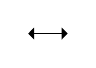
\begin{tikzpicture}
  \draw[black,  arrows={Triangle[angle=90:3pt,black,fill=black]-Triangle[angle=90:3pt,black,fill=black]}] (0,0.0) -- (0.5,0.0);   
\end{tikzpicture}\xspace}

\newcommand\edgethree{
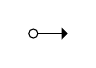
\begin{tikzpicture}
  \draw[black,  arrows={Circle[open]-Triangle[angle=90:3pt,black,fill=black]}] (0,0.0) -- (0.5,0.0);   
\end{tikzpicture}\xspace}

\newcommand\edgefour{
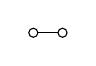
\begin{tikzpicture}
  \draw[black,  arrows={Circle[open]-Circle[open]}] (0,0.0) -- (0.5,0.0);   
\end{tikzpicture}\xspace}


% --- MATH MACROS ---
\newcommand\norm[1]{\left\lvert#1\right\lvert}
\usepackage{amsthm}
\DeclareMathOperator*{\argmax}{argmax}
\usepackage{thmtools}
\usepackage{tikz}
\usetikzlibrary{arrows.meta}
\declaretheoremstyle[headfont=\scshape]{schead}
\declaretheoremstyle[headfont=\bf]{bfhead}
\newcommand\independent{\protect\mathpalette{\protect\independenT}{\perp}}
\newcommand\notindependent{\not\independent}
\def\independenT#1#2{\mathrel{\rlap{$#1#2$}\mkern2mu{#1#2}}}
\declaretheorem[style=schead]{definition}
\declaretheorem[style=bfhead]{example}

% --- Algorithm ---
\usepackage[linesnumbered,ruled,vlined, noend]{algorithm2e}
\newcommand\mycommfont[1]{\footnotesize\ttfamily\textcolor{gray70}{#1}}
\SetCommentSty{mycommfont}
\SetAlCapNameFnt{\footnotesize}
\SetAlCapFnt{\footnotesize}
\SetAlgorithmName{Pseudocode}{Pseudocode}{Pseudocode of Algorithms}
\newcommand\algvar[1]{\texttt{#1}\xspace}
\newcommand\alginlinecomment[1]{\grayline{\hfill$\triangleright$~\textsl{#1}}\xspace}
\newcommand\algnestedcomment[1]{\javadocblue{$\triangleright$~\textsl{#1}}\xspace}
\newcommand\algcomment[1]{\javadocblue{$\triangleright$~\text{#1}\xspace}}

% --- Material style Result Box ---
\usepackage[framemethod=tikz]{mdframed}
\usetikzlibrary{shadows}
\usepackage{graphics}
\newmdenv[
    tikzsetting= {fill=gray05!0},
    skipabove=0.33em,
    skipbelow=0.33em,
    linewidth=1pt,
    innerleftmargin=4pt,
    innerrightmargin=4pt,
    innertopmargin=2pt,
    innerbottommargin=2pt,
    linecolor=gray85,
    roundcorner=2pt, 
    shadow=true,
    shadowsize=4pt,
    shadowcolor=black
]{myshadowbox}
\newmdenv[
    tikzsetting= {fill=gray05!0},
    skipabove=0.33em,
    skipbelow=0.33em,
    linewidth=1.25pt,
    innerleftmargin=4pt,
    innerrightmargin=4pt,
    innertopmargin=2pt,
    innerbottommargin=2pt,
    linecolor=gray85,
    roundcorner=3pt, 
    shadow=false,
    shadowsize=3pt,
    shadowcolor=black
]{mygoalbox}
\usepackage{tikz}
\newcommand*\circled[1]{\tikz[baseline=(char.base)]{
            \node[shape=circle,draw,inner sep=0.5pt] (char) {\small #1};}}

\newenvironment{result}
{\begin{myshadowbox}
  \besq
  \item[\faHandORight]
    % \item[]
  % \item[{\footnotesize \faPlay}]
  }
{\ee\end{myshadowbox}}

\newenvironment{goal}
{\vspace{0.2em}
\begin{mygoalbox}
  \besq
    % \item[\faHandORight]
    \item[{\footnotesize \faPlay}]
}
{
  \ee
  \end{mygoalbox}
}
%\renewcommand{\Bbbk}{\mathbb{k}}
%\setlength{\textfloatsep}{10pt plus 1.0pt minus 2.0pt}

\newcommand\given[1][]{\:#1\vert\:}

% --- ALGORITHMS ---
\newcommand{\algcauper}{%
\begingroup
\removelatexerror% Nullify \@latex@error
\begin{algorithm}[H]
    % \SetAlgoLined
    \footnotesize
    \SetKwInOut{Input}{Input}
    \SetKwInOut{Output}{Output}
    \SetKwFunction{Fframework}{\tool}
    \SetKwProg{Fn}{Function}{:}{}
    \Input{%
            $\mathrm{D}$: ~Observational Data\\
            $\mathbb{Y}_i$: ~Performance objective $\mathit{i}$\\
            $\mathrm{X}$: ~Intervenable configurations\\
            $\mathbb{Y}^{\mathit{fault}}_\mathit{i}$: ~Faulty Performance objective $\mathit{i}$\\
        %  $\mathrm{Z}$: ~Non-intervenable observable configurations.\\
            }
    \Output{%
        % $\mathcal{I}$:~ Interventions\\
        $\mathcal{C},~\mathcal{R}$:~ Root causes, Prescribed Changes.\\ 
    }
    % \Fn{\Fframework{$\mathbb{D}_\text{train}, \alpha, \beta, \gamma, lr$}}{
    \Fn{\Fframework}{
        % $\algvar{c\_paths} \leftarrow \varnothing$ \alginlinecomment{Causal}

        % $\algvar{interventions} \leftarrow \varnothing$ \alginlinecomment{Possible interventions}
                
        \algcomment{Contruct Causal Graphs}%\smallskip
        
        % \For(\alginlinecomment{Bootstrap resample}){$\mathrm{d} \in D.\mathit{resample()}$}{
        $\algvar{fci\_pag} \leftarrow \text{FCI}\left(\mathrm{D}\right)$ \alginlinecomment{Partial DAG with FCI.}\label{line:c_graph_0}
        
        $\algvar{ntr\_dag} \leftarrow \text{NOTEARS}\left(\mathrm{D}\right)$ \alginlinecomment{DAG with NOTEARS.}
        
        \smallskip\algcomment{Orient undirected edges.}

        $\algvar{c\_graph} \leftarrow \text{orient}\left(fci\_pag, ntr\_dag\right)$\label{line:c_graph_1}
        % }

        \smallskip\algcomment{Causal Path Discovery}%\smallskip
        
        \For{$perf\_obj \in \mathbb{Y}_i$}{ \label{line:c_paths_0}
            % \smallskip\algnestedcomment{All reachable nodes from performance objective.}
            
            $\algvar{c\_paths} \leftarrow  \text{get\_causal\_paths}\left(\mathrm{X},~\mathit{perf\_obj}\right)$
        }
        
        \smallskip\algcomment{Compute Average Causal Effect (ACE) of paths.}%\smallskip

        \For{$p \in c\_paths$}{
            \If{every $X \in p$ is \textsl{identifiable}}{  
                % \smallskip\algnestedcomment{Get average causal effect of all intervenable configurations in path.}
                $\algvar{p.ace} \leftarrow \text{average\_causal\_effect}\left(p\right)$
            }
        }
        
        
        $\algvar{top\_paths} \leftarrow \text{rank\_paths}\left(c\_paths,~\mathrm{K}\right)$\alginlinecomment{Select top $\mathrm{K}$ paths}\label{line:c_paths_1}\\
        \smallskip\algcomment{Generate interventions}

        % \For{$\mathit{path} \in \mathit{top\_paths}$}{
        %     \For{$\mathit{node} \in \mathit{path}$}{
        %         \algnestedcomment{set node to all permitted values}
        %     }
        % }
        $\algvar{intervene} \leftarrow \text{gen\_interventions}(\algvar{top\_paths},~\mathbb{Y}^{\mathit{fault}}_\mathit{i})$\label{line:intervene}
        

        \smallskip\algcomment{Find the intervention with maximum treatment effect}%\smallskip

        $\mathcal{I} \leftarrow \algvar{intervene.max(\green{"treatment~effect"})}$

        $\mathcal{C} \leftarrow \text{root\_causes}\left(\mathcal{I}\right)$ \algnestedcomment{Get the root-causes from intervention.}
        
        $\mathcal{R} \leftarrow \text{prescriptions}\left(\mathcal{C}\right)$ \algnestedcomment{Get prescriptions for the root-causes.}
        
        % \algcomment{Return root-causes and prescriptions.}%\smallskip

        \smallskip\Return $\mathcal{C}, \mathcal{R}$
    }
    \caption{\small Algorithmic outline of \tool}
    \label{alg:overview_psuedocode}    
\end{algorithm}
\endgroup}

\newcommand{\algquery}{%
\begingroup
\removelatexerror% Nullify \@latex@error
\begin{algorithm}[H]
    % \SetAlgoLined
    \footnotesize
    \SetKwInOut{Input}{Input}
    \SetKwInOut{Output}{Output}
    \SetKwFunction{Fframework}{gen\_interventions}
    \SetKwFunction{Frecurse}{recurse$\left(node\right)$}
    \SetKwFunction{FrecurseA}{recurse$\left(node.next(),~lst\right)$}
    \SetKwProg{Fn}{Function}{:}{}
    \Input{%
         $top\_paths$: ~Causal Paths from Performance Objectives\\\vspace{0.25em}
         $\mathbb{Y}^{\mathit{fault}}_\mathit{i}$: ~Faulty performance objectives\\\vspace{0.25em}
         $\mathbb{Y}^{\mathit{fixed}}_\mathit{i}$: ~\textsl{(Optional)} Performance objective to keep fixed\\\vspace{0.25em}
         }
    \Output{%
        $\mathit{intervene}$:~ Possible interventions on the provided paths\\
    }
    % % \Fn{\Fframework{$\mathbb{D}_\text{train}, \alpha, \beta, \gamma, lr$}}{
    \Fn{\Fframework} {

        \algcomment{Recursively enumerate all interventions on nodes in a path}
        \Fn{\Frecurse} {            
            \lIf(\alginlinecomment{Path end.}){$\text{node is } \mathbb{Y}^{~\mathit{fault}}_\mathit{~i}$}{  
                $\algvar{intervene} \leftarrow lst$
            } \Else(\alginlinecomment{Recurse with no change}){
                
                $\mathit{lst} \leftarrow node$

                \FrecurseA

                \algcomment{Recurse by changing node to all permitted values}

                \For{$new\_val \in node.allowed\_values$}{

                $\algvar{node.val} \leftarrow new\_val$ \alginlinecomment{Update node value}

                $\mathit{lst} \leftarrow node$ 

                \FrecurseA
                }
            }
        }
        
        $\algvar{intervene} \leftarrow \emptyset$
        
        \For(\alginlinecomment{Get all possible interventions.}){$\text{path} \in \text{top\_paths}$}{
            
            $\algvar{lst} \leftarrow \emptyset$
            
            $\algvar{start} \leftarrow \mathit{path.start\_node}$

            \FrecurseA
        }
        
        \Return{$\mathit{intervene}$}
    }
     \caption{\small Generating Interventions}
    \label{alg:interventions}    
\end{algorithm}
\endgroup}



% --- PDF, URL AND HYPERLINK PACKAGES ---
\usepackage{url}

\usepackage{titlesec}
% \acmConference[Preprint]{}{October, 2020}{ARXIV}
% \titlespacing{command}{left spacing}{before spacing}{after spacing}[right]
\author{Md Shahriar Iqbal}
% \authornote{Joint First Author}
\affiliation{%
  \institution{University of South Carolina}}
\email{miqbal@email.sc.edu}

\author{Rahul Krishna}
% \authornotemark[1]
\affiliation{%
  \institution{IBM Research}}
\email{rkrsn@ibm.com}

\author{Mohammad Ali Javidian}
\affiliation{%
  \institution{Purdue University}}
\email{mjavidia@purdue.edu}

\author{Baishakhi Ray}
\affiliation{%
  \institution{Columbia University}}
\email{rayb@cs.columbia.edu}

\author{Pooyan Jamshidi}
\affiliation{%
  \institution{University of South Carolina}}
 \email{pjamshid@cse.sc.edu}

\AtBeginDocument{%
  \providecommand\BibTeX{{%
    \normalfont B\kern-0.5em{\scshape i\kern-0.25em b}\kern-0.8em\TeX}}}

\copyrightyear{2022}
\acmYear{2022}
\setcopyright{rightsretained}
\acmConference[EuroSys '22]{Seventeenth European Conference on Computer Systems}{April 5--8, 2022}{RENNES, France}
\acmBooktitle{Seventeenth European Conference on Computer Systems (EuroSys '22), April 5--8, 2022, RENNES, France}\acmDOI{10.1145/3492321.3519575}
\acmISBN{978-1-4503-9162-7/22/04}
\pagenumbering{gobble}
\begin{document}
% \title{\tool: Causal Debugging of Configuration Errors\\ to Fix Non-Functional Faults}
% --- ARXIV Title -----
% \title{\tool: A Causal Debugging Toolkit To Diagnose Misconfigurations}
%\title{\tool: A Systematic Method For Debugging Misconfigurations using Counterfactual Reasoning}
%\title{\tool: Performance Tasks of Composed Systems using Causal Inference}
% \title{Analyzing Performances of Composed Systems with Causal Inference}
\title{\ourapproach: Reasoning about Configurable System Performance through the Lens of Causality}

% \thispagestyle{plain}
% \pagestyle{plain}
\graphicspath{{figures-vg/}}
\begin{abstract}

Modern computer systems are highly configurable, with the total variability space sometimes larger than the number of atoms in the universe. Understanding and reasoning about the performance behavior of highly configurable systems, over a vast and variable space, is challenging. State-of-the-art methods for performance modeling and analyses rely on predictive machine learning models, therefore, they become (i)~\emph{unreliable in unseen environments} (e.g., different hardware, workloads), and (ii)~\emph{may produce incorrect explanations}. To tackle this, we propose a new method, called \ourapproach, which (i)~\emph{captures intricate interactions} between configuration options across the software-hardware stack and (ii)~describes how such interactions can impact \emph{performance variations} via causal inference. We evaluated \ourapproach on six highly configurable systems, including three on-device machine learning systems, a video encoder, a database management system, and a data analytics pipeline. The experimental results indicate that \ourapproach outperforms state-of-the-art performance debugging and optimization methods in finding effective repairs for performance faults and finding configurations with near-optimal performance. Further, unlike the existing methods, the learned causal performance models reliably predict performance for new environments.  

\end{abstract}
    


% Context
% 
% Modern computer systems are highly configurable and are composed of heterogeneous components with variability space larger than the number of atoms in the universe. As a result of the ample variability space, the performance behavior of such systems becomes complex and, therefore, downstream performance-related tasks at operation time become challenging.


% Given a limited sampling budget, \ourapproach iteratively updates the learned performance model by estimating the causal effects of configuration options on performance objectives, then selecting the highest-impact options to adjust in order to address performance issues by improving the performance objective of interest without deteriorating other objectives in debugging task or recommend a near-optimal configuration. 
 


% Then, it uses them to \emph{explain} how such interactions impact the variation in performance objectives causally.

% even if they predict performance for the environment where configurations are measured, since they may infer correlations as causation, they typically do not transfer well for predicting system performance behavior in a new environment (e.g., change of hardware from the canary environment to production). 

% %The configuration options interact with each other within and across the system stack, and such interactions typically vary in different deployment environments or workload conditions. So, it becomes almost impossible to track down configuration options that should be set to different values to improve performance if the system's performance shows wide variability during operation time. 
%to become accurate for performance predictions in an environment, 
% The main problem here we address is to understand {\em why} the performance degradation is happening and {\em reason} based on a reliable model to improve it. This paper addresses this problem with the causal inference approach---where we try to reason about the interactions among configuration options, systems events, and systems performance. 

% The main problem we address here is to understand {\em why} the performance degradation is happening and {\em reason} based on a reliable model to improve it.
% To this end, this paper proposes a new methodology, called \ourapproach, which initially learns a Causal Performance Model to reliably \emph{capture intricate interactions} between options across the software-hardware stack by tracing system-level performance events across the stack (hardware, software, cache, and trace point). Then, it uses them to \emph{explain} how such interactions impact the variation in performance objectives causally. Given a limited sampling budget, \ourapproach iteratively updates the learned performance model by estimating the causal effects of configuration options on performance objectives, then selecting the highest-impact options to adjust in order to address performance issues by improving the performance objective of interest without deteriorating other objectives in debugging task or recommend a near-optimal configuration. 

%as intermediate causal mechanisms
% Leveraging such performance model, \ourapproach further facilitates performance tasks such as tuning, debugging, and optimization by estimating the causal effects of configuration options to performance objectives.
%Leveraging such performance model, \ourapproach further facilitates performance tasks such as tuning, debugging, and optimization, based on the learned causal performance model via. 

% To this end, we show that we can reliably \emph{capture intricate interactions} between options across software-hardware stack by tracing system-level performance events across the stack (hardware, software, cache, and tracepoint) and used them as intermediate causal mechanisms. 

% that facilitates downstream performance tasks such as performance tuning, debugging, and optimization by employing a unified causal analysis approach. Our methodology first recovers the underlying causal structure that encodes how configuration options and their interactions influence performance objectives from system performance measurements. Then, using the mathematical foundation of causality, \ourapproach derives quantities of interests in the downstream performance tasks. For instance, \ourapproach calculates the causal effects of configuration options to the performance objectives by searching over the learned causal structure, which enables users to not only \emph{identify} the root cause of a performance fault, but also \emph{explain} and \emph{fix} the fault in a principled fashion. 

% We evaluated \ourapproach on six highly configurable systems, including three on-device machine learning systems, a video encoder, a database, and a data analytics pipeline. In addition, we compared the results with state-of-the-art configuration optimization and debugging methods. The experimental results indicate that \ourapproach can find effective repairs for performance faults and find configurations with near-optimal performance. Furthermore, unlike the existing methods, the learned causal performance models reliably predict performance for new environments where it has not been used during the learning process.  

% does not require measuring performance every time the deployment environment, workload, or task changes, as it relies on the learned causal model that remains stable given these frequent changes. 


% identifies root causes more accurately compared with statistical debugging approaches and offers competitive repairs compared with performance optimization approaches.

% can find effective repairs for faults in multiple non-functional properties with 21\% more accuracy and15\% higher gain than other ML-based performance debugging methods. Compared to multi-objective optimization approaches, \tool can find repairs $9×$ faster with comparable performance gain.

% We find that \tool can identify root causes more accurately compared to other approaches with $22.16\%$ better accuracy. Compared to optimization methods (SMAC), \tool repairs misconfigurations $85.21\%$ times faster while recommending fixes that perform as well as (or $4.43\%$ better than) the near-optima found by SMAC. \tool also repairs misconfigurations with multiple simultaneous non-functional faults (in latency, energy usage, and thermal output) with $21.65\%$ better accuracy in finding the root cause and repairs with $20.13\%$ better performance than other methods. Our case study of non-functional faults reported in NVIDIA's forum shows that \tool can find $26.56\%$ better repairs than the experts' advice; it does so $12\times$ faster. 

\begin{CCSXML}
<ccs2012>
   <concept>
       <concept_id>10011007.10011006.10011071</concept_id>
       <concept_desc>Software and its engineering~Software configuration management and version control systems</concept_desc>
       <concept_significance>500</concept_significance>
       </concept>
   <concept>
       <concept_id>10011007.10011074.10011784</concept_id>
       <concept_desc>Software and its engineering~Search-based software engineering</concept_desc>
       <concept_significance>500</concept_significance>
       </concept>
 </ccs2012>
\end{CCSXML}
\ccsdesc[500]{Software and its engineering~Software configuration management and version control systems}
\ccsdesc[500]{Software and its engineering~Search-based software engineering}
\keywords{Configurable Systems, Performance Modeling, Performance Debugging, Performance Optimization,  Causal Inference, Counterfactual Reasoning}
\maketitle

\section{Introduction}
% \begin{comment}
% Modern software systems are not only highly configurable but also being increasingly deployed on heterogeneous hardware environments such as system-on-chip (SoCs), consumer hardware, high-performance computing platforms (see ~\fig{sw_hw_stack}). Similar to the variability in the software code (activated based on configuration options \cite{xu2015hey, medeiros2016comparison, halin2019test}), there exists even much variability in the underlying hardware \cite{apel3feature, siegmund2015performance, xu2013not},  which is oblivious to software developers. 
% As a result, unexpected interactions between software and hardware result in transient non-functional faults even for systems where such non-functional faults have not been exhibited before in other hardware environments. 
% These non-functional faults do not resemble a typical software bug where the system crashes or exhibits obvious misbehavior. Instead, systems that have a non-functional fault are still functional but may either be compromised or may operate with degraded performance. As a result, as much as 99\% of the non-functional faults that arise due to misconfigurations go unreported~\cite{99ofmisc75:online}. These may have undesirable side-effects such as potential data breaches~\cite{Cloudmis78:online, YoureOne98:online}, high-latency, low throughput, or increased energy consumption~\cite{bryant2003computer, molyneaux2009art,Nistor2015,sanchez2020tandem}. Therefore, it is important to \emph{identify the root cause} of such faults and \emph{fix} them early and in a principled way.

% Such non-functional faults happen when the software has been shipped to the customers in situations where customers run such a system on a hardware platform that has never been tested before. Such non-functional faults may result in unresponsiveness of the system, excessive usage of energy, heat dissipations, and in several cases damaging the underlying hardware [complete the list]. Therefore, it is important to \emph{identify the root cause} of such faults and \emph{fix} early and in a principled way.

% However, it is extremely challenging to \emph{localize the root causes} of such faults and \emph{find a fix} for them. This is due to the huge configuration space, which is exponentially larger than only the software configuration space as a result of software-hardware interactions. The complex interactions between the configuration options in the software and their interactions with the underlying hardware options result in combinatorially large configuration space. Consequently, inspecting this vast space to identify what caused the non-functional fault can be very challenging. Expecting a developer to understand all these complex interactions and fixing the performance issue is impractical and in most cases impossible because the underlying hardware of the end-users is not known to the developers. % (see \tion{motivation} for several real examples of non-functional faults that occurred as a result of these intrinsic interactions). 



% Prior research provides many different performance debugging approaches to help developer to (i) identify the bugs \cite{Nistor2015, jin2012understanding, han2016emprical}, (ii) identify root causes of the bugs non-functional faults \cite{attariyan2012x, xuan2018genetic}, and (iii) find potential fixes \cite{Nistor2015, wang2018understanding}. 
% Statistical Debugging \cite{song2014statistical, andrzejewski2007statistical} uses data to capture faults by generating predicates and reasoning based on statistical methods to identify the most likely root causes of the fault by detecting predicates that are highly ``correlated'' with the failure. Statistical debugging approaches are highly dependent on data and typically produce many false negatives due to heavily relying on correlations instead of true causes of faults. 
% In this work, we instead, focus on ``causation'' to find a causally related source of the fault. 

% We evaluated \tool based on the effectiveness in discovering root causes of non-functional faults and finding fixes in (i) single objective (), (ii) multi-objective (), and (ii) transfer learning scenarios () and compared with a statistical debugging and a popular heuristic approach in 5 large-scale highly-configurable systems deployed in 4 different hardware platforms [check these are correct?]. We found that, on average, ....

% We also need to talk about the few causal approaches we know and position them properly here.
% \end{comment}

% % ------------------------------------------
% % --------------- VERSION 2 ----------------
% % ------------------------------------------

% \begin{figure}[t]
%     \setlength{\belowcaptionskip}{-1.25em}
%     \centering
%     \includegraphics[width=0.3\linewidth]{fig__intro_a.pdf}
%     \includegraphics[width=0.3\linewidth]{fig__intro_b.pdf}
%     \includegraphics[width=0.3\linewidth]{fig__intro_c.pdf}
%     \caption{\small{Simple example showing the effectiveness of causality in reasoning about system performance behavior. 
%     (a)  Observational data in shows that the increase in \texttt{Cache Misses} % \gpugrowth
%     leads to high \texttt{Throughput} and such trend is typically captured by statistical reasoning in ML models; (b) incorporating \texttt{Cache Policy} as a confounder correctly shows increase of \texttt{Cache Misses} correspond to decrease in \texttt{Throughput}; (c) the corresponding causal model capture \texttt{Cache Policy} as a common cause and explains performance behavior correctly.}}
%     \label{fig:intro_fig}\
% \end{figure}
 \begin{figure}[tp!]
  \subfloat[]{
	\begin{minipage}[c][1\width]{
	   0.3\linewidth}
	   \centering
	   \includegraphics[width=\textwidth]{figures-vg/fig__intro_a.pdf}
	\end{minipage}}
 \hfill 	
  \subfloat[]{
	\begin{minipage}[c][1\width]{
	   0.3\linewidth}
	   \centering
	   \includegraphics[width=\textwidth]{figures-vg/fig__intro_b.pdf}
	\end{minipage}}
 \hfill	
  \subfloat[]{
	\begin{minipage}[c][1\width]{
	   0.3\linewidth}
	   \centering
	   \includegraphics[width=\textwidth]{figures-vg/fig__intro_c.pdf}
	\end{minipage}}
\caption{\small{An example showing the effectiveness of causality in reasoning about system performance behavior. 
    (a)  Observational data shows that the increase in \texttt{Cache Misses} % \gpugrowth
    leads to high \texttt{Throughput} and such trend is typically captured by statistical reasoning in ML models; (b) incorporating \texttt{Cache Policy} as a confounder correctly shows increase of \texttt{Cache Misses} corresponding to decrease in \texttt{Throughput}; (c) the corresponding causal model correctly captures \texttt{Cache Policy} as a common cause to explain performance behavior.}}
    \label{fig:intro_fig}
\end{figure}

Modern computer systems, such as data analytics pipelines, are typically composed of multiple components, where each component has a plethora of configuration options that can be deployed individually or in conjunction with other components on different hardware platforms. The configuration space of such highly configurable systems is combinatorially large, with 100s if not 1000s of software and hardware configuration options that interact non-trivially with one another~\cite{wang2018understanding,halin2019test,JC:MASCOTS16,velez2022study}. Individual component developers typically have a relatively localized, and thus limited, understanding of the performance behavior of the systems that comprise the components. Therefore, developers and end-users of the final system are often overwhelmed with the complexity of composing and configuring components, making it challenging and error-prone to configure these systems to reach desired performance goals.




% As users ask  for more control, more configuration options are added over time, which by implication leads to more complexity. For example, an \textsc{HBase} administrator accidentally disables the \texttt{WAL} option assuming in-memory data will be periodically flushed to the disk. However, \textsc{HBase} does not do so when \texttt{WAL} is disabled. After learning that the \textsc{HBase} users lost the entire 2 weeks of data, \textsc{HBase} developers added more options to prevent the case to happen again~\cite{wal_issue:online} that would control the behavior of \texttt{Memstore flush queue} and \texttt{Compaction queue}. However, these additional configuration options result in severe write latency if not configured correctly~\cite{compaction:online}. 

% Existing approaches for performance debugging only solve half the problem: Performance debugging requires determining \textit{``why''} certain events, such as high latency or resource usage, happened in a system. Yet, most current tools, such as profilers and logging, only determine \textit{``what''} events happened during a performance anomaly. Existing performance analysis and debugging methods cannot recover the true underlying causes of performance faults as they are based on correlation-based statistics and, therefore, fixes may be ineffective or misleading. 

Incorrect configuration (\textit{misconfiguration}) elicits unexpected interactions between software and hardware, resulting in \textit{non-functional faults}\footnote{ \emph{Non-functional} and \emph{Performance faults} are used interchangeably to refer to severe performance degradation caused by certain type of misconfigurations, (aka. specious configuration)~\cite{hu2020automated}.}, \ie, degradations in \textit{non-functional} system properties like latency and energy consumption. These non-functional faults, unlike regular software bugs, do not cause the system to crash or exhibit any obvious misbehavior~\cite{reddy2016fault, tsakiltsidis2016automatic, nistor2013discovering}. Instead, misconfigured systems remain operational but degrade in performance~\cite{bryant2003computer, molyneaux2009art,sanchez2020tandem,nistor2015caramel} that can cause major issues in cloud infrastructure~\cite{amazon:config:outage}, internet-scale systems~\cite{fb:config:outage}, and on-device machine learning (ML) systems~\cite{slowimag79:online}. For example, a developer complained that \textit{``I have a complicated system composed of multiple components running on NVIDIA Nano and using several sensors and I observed several performance issues.~\cite{super_frustrated_power_perf:online}.''} 
In another instance, a developer asks \textit{``I’m quite upset with CPU usage on Jetson TX2 while running TCP/IP upload test program''~\cite{HighCPUu7:online}}. 
After struggling in fixing the issues over several days, the developer concludes, \textit{``there is a lot of knowledge required to optimize the network stack and measure CPU load correctly. I tried to play with every configuration option explained in the kernel documents.''}
In addition, they would like to \emph{understand} the impact of configuration options and their interactions, e.g., \textit{``What is the effect of swap memory on increasing throughput?~\cite{slowimag79:online}''}. 

%The developer has spent many hours collecting many event traces using utilities such as \emph{perf} to find out about the root causes of the performance degradation and comparing the statistics with other hardware platforms: \textit{``Seems like CPU usage on Jetson’s side is two times higher comparing with old FriendlyArm’s H5 CPU for the same task.''}
%This developer also formed some hypotheses:
% \textit{``Is this performance issue related to the old 4.9 kernels, or this is a driver-side issue or something else?''}
% % \begin{figure}[t!]
    % \setlength{\belowcaptionskip}{-3em}
    \centering
    \includegraphics*[width=\linewidth]{UnicornOverview}
    \caption{\small {Overview of \ourapproach}}
    \vspace{-2em}
    \label{fig:overview}
    % \rayb{I have questions about this figure. Let's talk in the morning}
\end{figure}

% Misconfigurations are responsible for 10$\%$ of the service outages or performance reduction in cloud deployments~\cite{gunawi2016does} that is considered to be the $4^{th}$ largest category among the faults that reside on the cloud~\cite{gunawi2014bugs}. These faults can easily cripple down numerous other services leaving behind many furious and frustrated users~\cite{xbox}. 
% As a result, non-functional faults arise in deployments even if such a fault was never previously encountered elsewhere~\needcitation. 
% 
\begin{figure}[t]
    \setlength{\belowcaptionskip}{-1.25em}
    \centering
    \includegraphics[width=\linewidth]{fig__intro_a.pdf}
    \caption{Observational data (in Fig.~\protect\ref{fig:intro_fig}a)  (incorrectly) shows that high \gpugrowth leads to high latency. The trend is reversed when the data is segregated by \swapmem.}
    \label{fig:intro_fig}
\end{figure}

% \begin{figure}[tp!]
%     \setlength{\belowcaptionskip}{-0.8em}
%     \centering
%     \subfloat[\gpugrowth v. Latency]
%     {\label{fig:intro_a}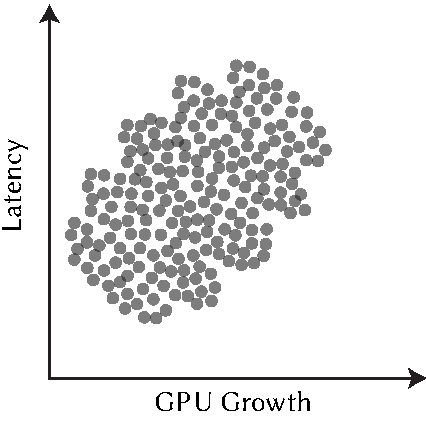
\includegraphics[width=0.45\linewidth]{fig__intro_1.pdf}}~
%     \subfloat[Observations segregated on \swapmem]
%     {\label{fig:intro_b}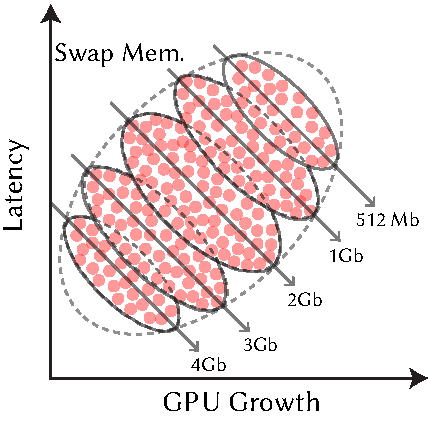
\includegraphics[width=0.45\linewidth]{fig__intro_2.pdf}}
%     \\[0.05em]
%     % \subfloat[Performance curves][Performance (Latency) curves]
%     % {\label{fig:intro_b}\includegraphics[width=0.68\linewidth]{fig__intro_b.pdf}}
%     \subfloat[][Causal Model]
%     {\label{fig:intro_c}\includegraphics[width=0.3\linewidth]{fig__intro_c.pdf}}\\[-1em]
%     \caption{\smallObservational data can sometimes lead to misleading inference. In \protectFig.~\ref{fig:intro_fig}a, the data (incorrectly) shows that high \gpugrowth leads to high latency. In \protectFig.~\ref{fig:intro_fig}b, the trend is reversed when the same data is segregated by \swapmem.}
%     \label{fig:intro_fig}
% \end{figure}

% Consequently, identifying the root cause of performance faults is notoriously difficult~\cite{gunawi2018fail} with as much as 99\% of them going unnoticed or unreported for extended durations~\cite{99ofmisc75:online}. This has tremendous monetary repercussions costing companies worldwide an estimated \$5 trillion in 2018 and 2019~\cite{Cloudmis78:online}. 


% ; or when they want to reason about performance in a different environment: \textit{``I’m trying to see how much faster the TX2 can classify images with TensorFlow than a Raspberry Pi model 3. My TensorFlow model was developed with transfer learning from the InceptionV3 CNN. My RPi takes about 20 seconds to classify an image, and to my surprise, the TX2 also takes about 20 seconds.~\cite{slowimag79:online}''}  
% \rayb{There are too many examples, we can reduce them to 1/2}
% Often developers are just curious to know whether an issue is arising due to misconfiguration, such as ~``\textit{I saw the latency is over 100ms, I am wondering if there is something misconfiguration or problems?~\cite{curious_issue:online}}.'' 
% The sheer number of modalities of software deployment is so large that exhaustively testing every conceivable software and hardware configuration is impossible!. 
% Crucially, these exchanges provoke other unanswered questions, such as ~``\textit{what would be the effect of changing another configuration `X'?~\cite{slowimag79:online}}.'' 

% Therefore, we seek methods that can \emph{identify, explain, and fix} the root cause of non-functional faults early in a principled fashion.


% \noindent\textbf{Existing work.}~
% Much recent work has focused on configuration optimization, which are approaches aimed at finding a configuration that optimizes a performance objective~\cite{wu2015deep, yigitbasi2013towards,siegmund2015performance, nair2018faster, filieri2015automated}. Finding the optimum configuration using push-button optimization approaches is not applicable here because they do not give us any information about the underlying interactions between the faulty configuration options that caused the non-functional fault. This information is sought after by developers seeking to address these non-functional faults~\cite{reddy2016fault, thung2012empirical}. 

\noindent\textbf{Existing works and gap.} Understanding the performance behavior of configurable systems can enable (i) performance debugging~\cite{SGAK:ESECFSE15,GSKA:SPPEXA}, (ii) performance tuning~\cite{H:CACM,SHM:LIO,H:AS,VPGFC:ICPE17,HPHL:ICSE15,WWHJK:GECCO15,NMSA:Arxive17,MARC:SPLC13,ORGC:SPLC14}, and (iii) architecture adaptation~\cite{JGAP:CSMR13,ABDD:VISSOFT13,KK:WSR16,JVKSK:SEAMS17,HSCMAR:SIGPLAN,FHM:FSE15,EEM:TSE,EEM:FSE10}. 
A common strategy is to build performance influence models such as regression models that explain the influence of individual options and their interactions~\cite{SGAK:ESECFSE15,VPGFC:ICPE17,GCASW:ASE13,pereira2019learning}. These approaches are adept at inferring the correlations between configuration options and performance objectives, however, as illustrated in~\fig{intro_fig} performance influence models suffer from several shortcomings (detailed in \S\ref{sec:motivation}): (i) they become ~\emph{unreliable in unseen environments} and (ii) ~\emph{produce incorrect explanations}.

% $f(c)=\beta_0+\Sigma_{i}{\phi(o_i)}+\Sigma_{i..j}{\phi(o_i..o_j)}$
% they lack the mathematical language to express \textit{how} the configuration options affect performance objectives. Without this, we risk drawing misleading conclusions. They also require significant time to gather the training samples, which grows exponentially with the number of configurations~\cite{kanellis2020too,xu2015hey}.  

% Prior work focuses on constructing performance influence models using machine learning or optimization methods~\cite{wu2015deep, yigitbasi2013towards, zhang2015performance,siegmund2015performance, nair2018faster, filieri2015automated, iqbal2020flexibo, jamshidi2016uncertainty}. These techniques cannot be used to diagnose and repair non-functional faults. There are several reasons for this. Firstly, these are usually pushbutton approaches that provide a one-size-fits-all optimal configuration that is very sensitive to minor changes to the system (\eg, slightly different workloads)~\cite{}. Secondly, they are adept at describing \textit{if} certain configuration options influence performance, however, they lack the mathematical language to express \textit{how} or \textit{why} the configuration options affect performance, without this, we risk drawing misleading conclusions. Lastly; they require significant time to gather the necessary measurements, and this grows exponentially with the number of configurations~\cite{}.  

% \noindent\textbf{Limitations of existing work.}~
% In \fig{intro_fig}, we present an example to help illustrate the limitations with current techniques. Here, the observational data gathered so far indicates that \gpugrowth is positively correlated with increased latency (as in Fig.~\ref{fig:intro_fig}a). An ML model built on this data will, with high confidence, predict that larger \gpugrowth leads to larger latency. However, this is counter-intuitive because higher \gpugrowth should, in theory, reduce latency not increase it. When we segregate the same data on \swapmem (as in~Fig.~\ref{fig:intro_fig}b), we see that there is indeed a general trend downward for latency, \ie, within each group of \swapmem, as \gpugrowth increases the latency decreases.
% We expect this because \gpugrowth controls how much memory the GPU can ``borrow'' from the \swapmem. Depending on resource pressure imposed by other host processes, a resource manager may arbitrarily re-allocate some \swapmem; this means the GPU borrows proportionately more/less swap memory thereby affecting the latency correspondingly. This is reflected by the data in Fig.~\ref{fig:intro_fig}b. If the ML-based model were to consult the available data (from Fig.~\ref{fig:intro_fig}a) unaware of such underlying factors, these models would be incorrect.
% With thousands of configurations, inferring such nuanced information from optimization or ML-based approaches would require a considerable amount of measurements and extensive domain expertise which can be impractical, if not impossible, to possess in practice.

% When we measure the latency by varying the \swapmem (and keeping \gpugrowth fixed), we observe that the latency vs. \swapmem curve changes minimally. When we double the \gpugrowth from $33\%$ to $66\%$, we observe a similar trend (Fig.~\ref{fig:intro_fig}b, top row). Conversely, when we increase \gpugrowth (under fixed \swapmem), we observe a sharp decline in latency. When the \swapmem is doubled from $2Gb$ to $4Gb$, the improvement in latency is more pronounced (Fig.~\ref{fig:intro_fig}b, bottom row). 

% Merely changing \swapmem would not affect latency without also changing \gpugrowth accordingly. 
% Further, external factors, \eg, other host processes, may affect both these configuration options. 
% Current methods do not allow us to understand these relationships. 
% 

% Therefore, to alleviate developers' burden, it is important to develop better methods to \emph{identify the root cause} of non-functional faults and \emph{fix} them early and in a principled way. % can be quite useful for software developers and system administrators.


% Statistical methods rely on simple ``correlation'' to draw their conclusions; these are heavily biased by the amount of available data resulting in a large number of false positives~\cite{}. \shariar{better example}For instance, correlation-based methods may highlight that certain \textit{scheduler policies} are correlated with high latency, however, they do not inform us if changing the scheduler policy alone can \textit{cause} the latency to improve. % can be quite useful for software developers and system administrators.

\noindent\textbf{Our approach.}~
Based on the several experimental pieces of evidence presented in the following sections, this paper proposes \ourapproach--a methodology that enables reasoning about configurable system performance with causal inference and counterfactual reasoning. \ourapproach first recovers the underlying causal structure from performance data. The causal performance model %instead of a performance model that has been learned using the mainstream regression-based approaches, 
allows users to (i)~identify the root causes of performance faults, (ii)~estimate the causal effects of various configurable parameters on the performance objectives, and (iii)~prescribe candidate configurations to fix the performance fault or optimize system performance. 
% 
% we propose the use of causal models~\cite{pearl2000models, pearl2009causality} to express the complex interactions between the configurations and the performance objectives with a rich graphical representation. Then, using counterfactual reasoning~\cite{pearl2011algorithmization} we identify the root cause of non-functional faults and prescribe repairs to fix the misconfigured options.
% 
% The causal model would also highlight that other hidden factors (\eg, other processes running on the host) may affect the configurations (shown by \circled{?} in Fig.~\ref{fig:intro_fig}c). 
% 
% To this end, 
% 

% For example, in~\fig{intro_fig}, \tool constructs a \textit{causal model} from observational data (as in Fig.~\ref{fig:intro_fig}c). This causal model indicates that \gpugrowth indirectly influences latency (via a \swapmem) and that the configuration options may be affected by certain other factors, \eg, resource manager allocating resources for other processes running on the host. \tool uses counterfactual questions such as, ``what is the effect of \gpugrowth on latency if the available \swapmem was 2Gb?'' to diagnose the faults and recommend changes to the configuration options to mitigate these faults. 


% \noindent\textbf{Evaluation.}~
% We evaluated \ourapproach in terms of its \emph{effectiveness, sample efficiency}, and \emph{scalability} and compared with state-of-the-art performance debugging and optimization using 5 real-world highly configurable systems (three machine learning systems, a video encoder, and a database system) deployed on 3 architecturally different NVIDIA Jetson devices. 

% We compare \ourapproach with state-of-the-art configuration optimization and ML-based performance debugging approaches. Overall, we find that \ourapproach is (at most) $13\times$ faster with $13\%$ better accuracy and $32\%$ higher gain than the next best ML-based approaches for single-objective faults. Compared to single-objective optimization approaches, \ourapproach can find repairs to misconfigurations $9\times$ faster while performing as well as (or better than) the best configuration discovered by the optimization techniques. Further, \ourapproach can find effective repairs for faults in multiple performance objectives (\ie, latency and energy consumption) with accuracy and gain as high as $16\%$ and $36\%$, respectively, than other ML-based performance debugging methods. Compared to multi-objective optimization approaches, \ourapproach can find repairs $5\times$ faster while having similar performance gain. Finally, with a case study, we demonstrate that \ourapproach finds $14\%$ better repairs than the experts' advice in 24 minutes.

% \tool would alleviate developers' burden, it is important to develop better methods to \emph{identify the root cause} of non-functional faults and \emph{fix} them early and in a principled way.
% If the prescribed repairs do not result in satisfactory performance improvement, \tool updates the causal model with new observations and repeats the above steps until the performance objective has been met. 

% Advise against the use of optimization:
%  - Don't want the global optima, but the original configuration with the smallest change to reach the performance objective. 
% - It does not give us any information on the underlying causality of the system. The explainability/expressiveness is lost -- we won't know how/why a certain change is useful. 
% Our work is tangentially related to other work on performance modeling and optimization of highly configurable systems using machine learning and optimization \cite{wu2015deep, yigitbasi2013towards, zhang2015performance,siegmund2015performance, nair2018faster, filieri2015automated, iqbal2020flexibo, jamshidi2016uncertainty}. These methods are designed as push-button solutions to offer a near-optimal configuration, they do not offer Here we essentially tackle a different problem---that of finding the root causes of an already observed non-functional fault and finding a fix for it instead of finding an optimization.

% , static and dynamic software analysis \cite{kim2013splat, meinicke2016essential, velez2019configcrusher, abal2018variability, nguyen2016igen}, or sampling techniques \cite{sarkar2015cost, siegmund2015performance, guo2013variability, jamshidi2018learning}.

% % \bi[leftmargin=*]
%     \noindent \textbf{Technique.} Our approach is the first to exploit causal inference and counterfactual reasoning to reason about the root causes for non-functional faults and offer repairs to fix them. 
%     % Our approach achieves this without actually performing any intervention (i.e., changing the configuration and deploying the system with the new configurations). This is unlike statistical debugging where we cannot reason about changes unless we have seen several failures to create discriminative models.

%     \noindent\textbf{Tool.} We propose \tool, a fully automated performance debugging approach that localizes the root causes of non-functional faults and fixes them. We show that \tool can handle faults in multiple performance objectives simultaneously. \tool is quite robust in that it can accommodate changes to software properties such as varying workloads. %We can reuse \tool to reason about non-functional faults in environments where we cannot collect new observations or we have only very few observational data. 

%     \noindent \textbf{Real-world Evaluation.} We evaluate \tool with 5 real-world highly configurable systems and it was able to identify the root causes and explain how the root causes (configuration options and interactions) triggered the fault, much more accurately with much less false negative compared with statistical debugging and the most popular heuristic approach in practice.
% % \ei



% \red{  Optimization tells us to configure under a certain way until the budget is finished. Need to collect new data to refine our estimate (bayesian opt) }
% \red{Analytical models require understanding and modeling of the system internal, which is impossible or expensive + data}
\begin{figure}[tp!]
    \centering
    \includegraphics*[width=\linewidth]{DeepStream-Arch.pdf}
    \caption{\small{\textsc{Deepstream}: An example of a highly-configurable composed system, a big data analytics pipeline system, with several configurable components: (i) Video Decoder performs video encoding/decoding with different formats; (ii) Stream Muxer accepts input streams and converts them to sequential batch frames; (iii) Primary Detector transforms the input frames based on input NN requirements and makes model inference to detect objects; (iv) Object Tracker supports multi-object tracking; (v) Secondary Classifier improves performance by avoiding re-inferencing.}}
    \label{fig:deepstream_pipeline}
    \vspace{-4mm}
\end{figure}


% \red{In eqs.~\ref{eq:do} and~\ref{eq:ace}, $\mathbb{E}(Y~|~do(X=x))$ is \textit{not} the same as the ordinary conditional distribution $\mathbb{E}\left(Y~|~X=x\right)$. This is because $\mathbb{E}\left(Y~|~X=x\right)$ takes the original population, as is, and filters it gets the sub-population where $X=x$. If $X=x$ does not exist in the population, the value of $\mathbb{E}\left(Y~|~X=x\right)$ would be misleading. In contrast, $\mathbb{E}\left(Y~|~\mathit{do}\left(X=x\right)\right)$ uses do-calculus rules~\cite{} to infer the value of distribution even when $X=x$ has never been encountered before. }
\noindent\textbf{Contributions.}~Our contributions are as follows:
\begin{itemize}
    \item We propose \ourapproach (\S\ref{sec:methodology}), a novel approach that allows causal reasoning about system performance.
    % causal diagnostics, and fault mitigation tool that identifies the root causes of non-functional faults and recommends repairs to resolve non-functional faults.% using a novel entropy-based causal structure discovery followed by causal effect estimation and counterfactual reasoning.
    \item We \emph{have conducted a thorough evaluation} of \ourapproach in a controlled case study (\S\ref{sec:casestudy}) as well as real-world large-scale experiments. In particular, we evaluated \emph{effectiveness} (\S\ref{sec:effectiveness}), \emph{transferability} (\S\ref{sec:transfer}), and \emph{scalability} (\S\ref{sec:scalability}) by comparing \ourapproach with: (i)~state-of-the-art performance debugging approaches, including \textsc{CBI}~\cite{song2014statistical}, \textsc{DD}~\cite{artho2011iterative}, \textsc{EnCore}~\cite{zhang2014encore}, and \textsc{BugDoc}~\cite{lourencco2020bugdoc} and (ii)~performance optimization techniques, including \textsc{SMAC}~\cite{hutter2011sequential} and \textsc{PESMO} \cite{hernandez2016predictive}. The evaluations were conducted on six real-world highly configurable systems, including a video analytic pipeline, \textsc{Deepstream}~\cite{DeepStream}, three deep learning-based systems, \textsc{Xception} \cite{chollet2017xception}, \textsc{Deepspeech}~\cite{hannun2014deep}, and \textsc{BERT}~\cite{devlin2018bert}, a video encoder, X264~\cite{x264}, and a database engine, SQLite~\cite{SQLite}, deployed on \textsc{NVIDIA Jetson} hardware (\txone, \txtwo, and \xavier). \item In addition to sample efficiency and accuracy of \ourapproach in finding root causes of performance issues, we show that the learned causal performance model is transferable across different workload and deployment environments. Finally, we demonstrate the scalability of \ourapproach to large systems consisting of 500 options and several trillion potential configurations.  
    % Our empirical results, conducted on 5 highly configurable systems deployed on 3 architecturally different hardware, \tool outperforms current state-of-the-art ML-based (Correlational, Association Rule Mining, Decision Tree, Regression Tree, Classification based approaches) diagnostics and optimization approaches in terms of efficacy (+16\% accuracy and +36\% gain) and speed (up to 13$\times$ faster). \tool was also adept at handling both single- and multi-objective performance faults. 
    % \item We offer a manually curated performance fault dataset (called Jetson Faults) and accompanying code required to reproduce our findings at 
    \item The artifacts and supplementary materials can be found at \href{github}{\color{blue!80} https://github.com/softsys4ai/unicorn}.
\end{itemize}   


\section{Motivating Scenarios}
\label{sec:motivation}
\begin{figure}[tp!]
    % \setlength{\belowcaptionskip}{-1em}
    
 \subfloat[Performance Distribution]{\raisebox{-7.5em}{\includegraphics*[width=0.65\linewidth, valign=b]{fig__spread.pdf}}\label{fig:perf_behavior}} 
%  \qquad 
 \subfloat[Misconfiguration]{
        \resizebox{0.32\linewidth}{!}{\adjustbox{valign=m}{%
       \begin{tabular}{lV{2.5}rV{2.5}}
    \clineB{1-2}{2.5}
    \multicolumn{1}{V{2.5}lV{2.5}}{\textbf{Config. Option}}& {Value} \\ 
     \clineB{1-2}{2.5}
    \multicolumn{1}{l}{} & \multicolumn{1}{l}{} \\[-0.3em] \hlineB{2.5}
     
    \multicolumn{1}{V{2.5}lV{2.5}}{CPU Cores} & 2 \\

    \multicolumn{1}{V{2.5}lV{2.5}}{CPU Frequency (GHz)} & 0.1 \\

    \multicolumn{1}{V{2.5}lV{2.5}}{EMC Frequency (GHz)} & 1.6\\

    \multicolumn{1}{V{2.5}lV{2.5}}{GPU Frequency (GHz)} & 0.7\\

    \multicolumn{1}{V{2.5}lV{2.5}}{Scheduler Policy} & \textsc{noop}\\

    \multicolumn{1}{V{2.5}lV{2.5}}{Scheduler Runtime ($\mu$s)} &  950k \\

    \multicolumn{1}{V{2.5}lV{2.5}}{Scheduler Child Runs First} & 1 \\
    
     \multicolumn{1}{V{2.5}lV{2.5}}{Batched Push Timeout} & 1 \\
     
      \multicolumn{1}{V{2.5}lV{2.5}}{Batch Size} & 1 \\
      
      \multicolumn{1}{V{2.5}lV{2.5}}{Interval} & 1 \\
      
      \multicolumn{1}{V{2.5}lV{2.5}}{Buffer Size} & 6000 \\

    \multicolumn{1}{V{2.5}lV{2.5}}{ Dirty Background Ratio} & 5 \\

    \multicolumn{1}{V{2.5}lV{2.5}}{Dirty Ratio} &  10  \\

    \multicolumn{1}{V{2.5}lV{2.5}}{Drop Caches}  &0  \\

    \multicolumn{1}{V{2.5}lV{2.5}}{Cache Pressure} & 500 \\
    
    \multicolumn{1}{V{2.5}lV{2.5}}{Swappiness} & 60  \\

    \multicolumn{1}{V{2.5}lV{2.5}}{Enable Padding} & 1 \\

    \multicolumn{1}{V{2.5}lV{2.5}}{Offset} & 0 \\
    
     \multicolumn{1}{V{2.5}lV{2.5}}{Swap Memory (Gb)} & 1 \\
     
      \multicolumn{1}{V{2.5}lV{2.5}}{Sched Time Avg (ms)} & 1000 \\
      
       \multicolumn{1}{V{2.5}lV{2.5}}{Dirty Bytes} & 30 \\
       
        \multicolumn{1}{V{2.5}lV{2.5}}{Overcommit Memory} & 2 \\
        
         \multicolumn{1}{V{2.5}lV{2.5}}{Overcommit Hugepages} & 1 \\
        
        
        
        
        
    \hlineB{2.5}

    \multicolumn{1}{l}{} & \multicolumn{1}{l}{}  \\[-0.9em] 
    \clineB{1-2}{2.5}
     
    \multicolumn{1}{V{2.5}lV{2.5}}{Throughput (FPS)} & 6.8 \\
       
    \multicolumn{1}{V{2.5}lV{2.5}}{Energy (J)} & 122 \\
     \clineB{1-2}{2.5}
        \end{tabular}}}
        \label{tab:example_fault}}

% %  
\caption{\small {(a) Performance distribution when \textsc{Deepstream} is deployed on NVIDIA Jetson Xavier (b) Misconfiguration that caused the multi-objective non-functional fault, shown as {\color{orange!60} $\square$} in the performance distribution.}}
\vspace{-3mm}
% \rayb{Parts of figure e is not clear. Let's talk in the morning. }
\label{tab:sample_fault}\end{figure}

% \begin{figure}[t!]
    
%     \centering
%     \resizebox{0.5\linewidth}{!}{%
%     \begin{tabular}{lV{2.5}r|}
%     \clineB{1-2}{2.5}
%     \multicolumn{1}{V{2.5}lV{2.5}}{\textbf{Configuration Options}}& {Values} \\ 
%      \clineB{1-2}{2.5}
%     \multicolumn{1}{l}{} & \multicolumn{1}{l}{}  \\[-0.9em] \hlineB{2.5}
     
%     \multicolumn{1}{V{2.5}lV{2.5}}{CPU Cores} & 2 \\

%     \multicolumn{1}{V{2.5}lV{2.5}}{CPU Frequency (GHz)} & 0.1 \\

%     \multicolumn{1}{V{2.5}lV{2.5}}{EMC Frequency (GHz)} & 1.6\\

%     \multicolumn{1}{V{2.5}lV{2.5}}{GPU Frequency (GHz)} & 0.7\\

%     \multicolumn{1}{V{2.5}lV{2.5}}{Scheduler Policy} & \textsc{noop}\\

%     \multicolumn{1}{V{2.5}lV{2.5}}{Scheduler Run Time ($\mu$s)} &  950000 \\

%     \multicolumn{1}{V{2.5}lV{2.5}}{Scheduler Child Runs First} & 1 \\

%     \multicolumn{1}{V{2.5}lV{2.5}}{Dirty Background Ratio} & 5 \\

%     \multicolumn{1}{V{2.5}lV{2.5}}{Dirty Ratio} &  10  \\

%     \multicolumn{1}{V{2.5}lV{2.5}}{Drop Caches}  &0  \\

%     \multicolumn{1}{V{2.5}lV{2.5}}{Cache Pressure} & 500 \\
    
%     \multicolumn{1}{V{2.5}lV{2.5}}{Swappiness} & 60  \\

%     \multicolumn{1}{V{2.5}lV{2.5}}{GPU Memory Growth} & default  \\

%     \multicolumn{1}{V{2.5}lV{2.5}}{Logical Devices} & 50 \\
    
%      \multicolumn{1}{V{2.5}lV{2.5}}{Swap Memory (Gb)} & 1 \\
%     \hlineB{2.5}

%     \multicolumn{1}{l}{} & \multicolumn{1}{l}{}  \\[-0.9em] 
%     \clineB{1-2}{2.5}
     
%     \multicolumn{1}{V{2.5}lV{2.5}}{Latency (sec)} & 152 \\
%      \clineB{1-2}{2.5}
% \end{tabular}}%


% \caption{\small \textcolor{blue}{An example of a misocnfiguration that led to a \textsc{nf-fault} due to latency.}}
% \label{fig:example_fault}
% \end{figure}

\noindent
\textbf{Simple motivating scenario.} In this simple scenario, we motivate our work by demonstrating why performance analyses solely based on correlational statistics may lead to an incorrect outcome. Here, the collected performance data indicates that \texttt{Throughput} is positively correlated with increased \texttt{Cache Misses}\footnote{we used a \texttt{distinct font} to indicate variables such as configuration options or performance metrics and events throughout this paper.} (as in  \fig{intro_fig}(a)). A simple ML model built on this data will predict with high confidence that larger \texttt{Cache Misses} leads to higher \texttt{Throughput}---this is misleading as higher \texttt{Cache Misses} should, in theory, lower \texttt{Throughput}. By further investigating the performance data, we noticed that the caching policy was automatically changed during measurement. We then segregated the same data on \texttt{Cache Policy} (as in~ \fig{intro_fig}(b)) and found out that within each group of \texttt{Cache Misses}, as \texttt{Cache Misses} increases, the \texttt{Throughput} decreases. One would expect such behavior, as the more \texttt{Cache Misses} the higher number of access to external memory, and, therefore, the \texttt{Throughput} would be expected to decrease. The system resource manager may change the \texttt{Cache Policy} based on some criteria; this means that for the same number of \texttt{Cache Misses}, the \texttt{Throughput} may be lower or higher; however, in all \texttt{Cache Policies}, the increases of \texttt{Cache Misses} resulting in a decrease in \texttt{Throughput}. Thus, \texttt{Cache Policy} acts as a confounder that explains the relation between \texttt{Cache Misses} and \texttt{Throughout}, which a correlation-based model will not be able to capture. In contrast, a causal performance model, as shown in \fig{intro_fig}(c), finds the relation between \texttt{Cache Misses}, \texttt{Cache Policy}, and \texttt{Throughput} and thus can reason about the observed behavior correctly. 

In reality, performance analysis and debugging of heterogeneous multi-component systems is non-trivial and often compared with finding the needle in the haystack~\cite{whitaker2004configuration}. In particular, the end-to-end performance analysis is not possible by reasoning about individual components in isolation, as components may interact with one another in such a composed system. Below, we use a highly configurable multi-stack system to motivate why causal reasoning is a better choice for understanding the performance behavior of complex systems. 

\noindent
\textbf{Motivating scenario based on a highly configurable data analytics system.} We deployed a data analytics pipeline, \textsc{Deepstream}~\cite{DeepStream}. \textsc{Deepstream} has many components, and each component has many configuration options, resulting in several variants of the same system as shown in~\fig{deepstream_pipeline}. Specifically, the variability arises from: 
(i)~the configuration options of each software component in the pipeline, (ii)~configurable low-level libraries that implement functionalities required by different components (e.g., the choice of tracking algorithm in the tracker or different neural network architectures), (iii)~the configuration options associated with each component's deployment stack (e.g., \texttt{CPU Frequency} of \xavier).  Further, there exist many configurable events that can be measured/observed at the OS level by the event tracing system. More specifically, the configuration space of the system includes (i) 27 Software options (Decoder: 6, Stream Muxer: 7, Detector: 10, Tracker: 4), (ii) 22 Kernel options (e.g., \texttt{Swappiness}, \texttt{Scheduler Policy}, etc.), and (iii) 4 Hardware options (\texttt{CPU Frequency}, \texttt{CPU Cores}, etc.). We use 8 camera streams as the workload, x264 as the decoder, TrafficCamNet model that uses ResNet 18 architecture for the detector, and an NvDCF tracker, which uses a correlation filter-based online discriminative learning algorithm for tracking. Such a large space of variability makes performance analysis challenging. This is further exacerbated by the fact that the configuration options among the components \emph{interact} with each other. Additional details about our \textsc{Deepstream} implementation can be found in the \href{https://github.com/softsys4ai/unicorn}{\color{blue!80}supplementary materials}.

To better understand the potential of the proposed approach, we measured (i) application performance metrics including throughput and energy consumption by instrumenting the \textsc{Deepstream} code, and (ii) 288 system-wide performance events (hardware, software, cache, and tracepoint) using $perf$ and measured performance for 2461 configurations of \textsc{Deepstream} in two different hardware environments, \xavier, and \txtwo.  As it is depicted in  \fig{perf_behavior}, performance behavior of \textsc{Deepstream}, like other highly configurable systems, is non-linear, multi-modal, and non-convex~\cite{jamshidi2016uncertainty}. In this work, we focus on two performance tasks: 
(i) \textit{Performance Debugging}: here, one observes a performance issue (e.g., latency), and the task involves replacing the current configurations in the deployed environment with another that fixes the observed performance issue; 
(ii) \textit{Performance Optimization}: here, no performance issue is observed; however, one wants to get a near-optimal performance by finding a configuration that enables the best trade-off in the multi-objective space (e.g., throughput vs. energy consumption vs. accuracy in \textsc{Deepstream}).

To show major shortcomings of existing state-of-the-art performance models, we built performance influence models that have extensively been used in the systems' literature~\cite{siegmund2015performance,JSVKPA:ASE17,GCASW:ASE13,GSKA:SPPEXA,kolesnikov2019tradeoffs,kaltenecker2020interplay,muhlbauer2019accurate,grebhahn2019predicting,siegmund2020dimensions} and it is the standard approach in industry~\cite{kolesnikov2019tradeoffs,kaltenecker2020interplay}. Specifically, we built non-linear regression models with forward and backward elimination using a step-wise training method on the \textsc{Deepstream} performance data. We then performed several sensitivity analyses and identified the following issues: 
\besq
    \item \textbf{Performance influence models could not reliably predict performance in unseen environments.} 
    Performance behavior of configurable systems vary across environments, e.g., when we deploy software on new hardware with a different microarchitecture or when the workload changes~\cite{JSVKPA:ASE17,JVKSK:SEAMS17,JVKS:FSE18,iqbal_transfer_2019,VPGFC:ICPE17}. When building a performance model, it is important to capture predictors that transfer well, i.e., remain \emph{stable} across environmental changes. The predictors in performance models are options ($o_i$) and interactions ($\phi(o_i..o_j)$) that appear in the explainable models of form $f(c)=\beta_0+\Sigma_{i}{\phi(o_i)}+\Sigma_{i..j}{\phi(o_i..o_j)}$. The transferability of performance predictors is expected from performance models since they are learned based on one environment (e.g., staging as the source environment) and are desirable to reliably predict performance in another environment (e.g., production as the target environment). 
    Therefore, if the predictors in a performance model become unstable, even if they produce accurate predictions in the current environment, there is no guarantee that it performs well in other environments, i.e., they become unreliable for performance predictions and performance optimizations due to large prediction errors. 
    To investigate how transferable performance influence models are across environments, we performed a thorough analysis when learning a performance model for \textsc{DeepStream} deployed on two different hardware platforms that have two different microarchitectures. Note that such environmental changes are common, and it is known that performance behavior changes when, in addition to a change in hardware resources (e.g., higher \texttt{CPU Frequency}), we have major differences in terms of architectural constructs~\cite{ding2021generalizable,curtsinger2013stabilizer}, also supported by a thorough empirical study~\cite{JSVKPA:ASE17}. The results in \fig{barplot_hw_change} (a) indicate that the number of stable predictors is too small for the total number of predictors that appear in the learned regression models. Additionally, the coefficients of the common predictors change across environments as shown in \fig{coeff_across_environments} making them unreliable to be resued in the new scenario.  
    
    % ~\rayb{why the prediction is unreliable even after all these things? what evidence do you have for unreliable prediction?}
    
% \begin{figure}[h]
% \small
%     % \setlength{\belowcaptionskip}{-3em}
%     \centering
%     \includegraphics*[width=\linewidth]{figures-vg/reg_eq_noise.pdf}
%     \caption{\small {Number of total terms, causal terms, and accuracy of regression model under different sample sizes.}}
%     \label{fig:deepstream_no_of_terms}
%     \begin{flushleft}
%   \end{flushleft}
%     % \rayb{It is not clear that this figure shows baseline results. Can we write the takeaway? }
% \end{figure}
    

    
    \item \textbf{Performance influence models could produce incorrect explanations.} In addition to performance predictions, where developers are interested to know the effect of configuration changes on performance objectives, they are also interested to estimate and explain the effect of a change in particular \emph{configuration options} (e.g., changing \texttt{Cache Policy}) toward performance variations. It is therefore desirable that the strength of the predictors in performance models, determined by their coefficients, remain consistent across environments~\cite{ding2021generalizable,JSVKPA:ASE17}.  
    In the context of our simple scenario in \fig{intro_fig}, the learned performance influence model indicates that $0.16 \times \texttt{Cache Misses}$ is the most influential term that determines throughput, however, the (causal) model in \fig{intro_fig}(c) show that the interactions between configuration option \texttt{Cache Policy} and system event \texttt{Cache Misses} is a more reliable predictor of the throughput, indicating that the performance influence model, due to relying on superficial correlational statistics, incorrectly explains factors that influence performance behavior of the system. The low Spearman rank correlation between predictors coefficients indicates that a performance model based on regression could be highly unstable and thus would produce unreliable explanations as well as unreliable estimation of the effect of change in specific options for performance debugging or optimization.
\ee

\begin{figure}[tp!]
\small
    \centering
    \includegraphics*[width=\linewidth]{figures-vg/barplot_hw_change.pdf}
    \caption{\small {(a) Performance influence models do not generalize well as the number of common terms, total terms and prediction error of these models change from source (\xavier) to target (\txtwo). The rank correlation between source and target is 0.07 (p-value=0.73).} (b) \small {Causal performance models generalize better as the number of common terms, total terms and prediction error of the structural does not change much from source (\xavier) to target (\txtwo). The rank correlation between source and target is 0.49 (p-value=0.76).}}
    \label{fig:barplot_hw_change}
\end{figure}

\begin{figure}[tp!]
\small
    \centering
    \includegraphics*[width=\linewidth]{figures-vg/coeff_diff.pdf}
    \caption{\small {Visualizing co-efficient differences from the source (\xavier) performance influence model to the target (\txtwo) performance influence model for the common terms for both options and interactions (shown by $\otimes$). }}
    \label{fig:coeff_across_environments}
    
\end{figure}

% Note that performance influence models are the most common models for performance analyses due to their simplicity and since they produce explainable models, they have extensively been used in the systems' literature~\cite{siegmund2015performance,JSVKPA:ASE17,GCASW:ASE13,GSKA:SPPEXA,kolesnikov2019tradeoffs,kaltenecker2020interplay,muhlbauer2019accurate,grebhahn2019predicting,siegmund2020dimensions} and it is the standard approach in industry~\cite{kolesnikov2019tradeoffs,kaltenecker2020interplay}. %We set the maximum degree of interactions to the number of options in the deployed system. 



% \rayb{I think we need to bring back the old GPU vs memory growth example or something similar to show the difference between causality and correlation. After that this whole section will make more sense. Right now this section is mostly about showing baseline does not work, but why they do not work is missing.}


% 
% \begin{itemize}
%     \item Performance influence models could produce unreliable predictions: (i) adding more data or less (a plot that you show the number of new terms, the disappearance of previous terms, and accuracy when you change the number of observations from 10-50-100-500-1000 by subsampling the current measurements), (ii) measurement noise (adding different levels of noise to signal and measuring the same parameters in the previous plot)
%     \item Unstable performance models: (i) workload change, (ii) hardware change, (iii) library updates (one plot showing the same plot as the previous one but for hardware, workload, and both changes)
%     \item Incorrect explanation based on non-causal correlations that affect both the influential options that affect performance behavior or root causes of a perf issue as well as incorrect fixes that are not stable across environments (a table where you list examples of interactions because of confounder, v shape, other scenarios that I discussed with you).
% \end{itemize}





% COMMENTED THINGS


%To better understand the scope of our work, we investigate, in the context of our motivating example, the limitations of existing performance approaches that rely on correlation-based methods.

% \rayb{This whole para should go to intro. We already motivate the problem, no need to repeat it again.}

% \rayb{the following two paras should be in intro}
% \textbf{Performance related challenges.} The exponential size of configuration space and complex constraints among configuration options make it challenging to find a configuration that performs as desired, therefore, many users rely on the default configurations~\cite{siegmund2015performance}, which is suboptimal in many deployment environments~\cite{JSVKPA:ASE17}. Even the developers of configurable systems often do not (fully) understand the performance behavior of such systems because software options typically interact with each other and more importantly with the ones underlying the software layers, making performance behavior very much customized to the user's environments. 

% \textbf{Existing approaches.} Understanding the performance behavior of configurable systems can enable (i) performance debugging~\cite{SGAK:ESECFSE15,GSKA:SPPEXA}, (ii) performance tuning~\cite{H:CACM,SHM:LIO,H:AS,VPGFC:ICPE17,HPHL:ICSE15,WWHJK:GECCO15,NMSA:Arxive17,MARC:SPLC13,ORGC:SPLC14}, and (iii) architecture adaptation~\cite{JGAP:CSMR13,ABDD:VISSOFT13,KK:WSR16,JVKSK:SEAMS17,HSCMAR:SIGPLAN,FHM:FSE15,EEM:TSE,EEM:FSE10}. 
% A common strategy to build performance influence models in which regression-based models, of the form $f(c)=\beta_0+\Sigma_{i}{\phi(o_i)}+\Sigma_{i..j}{\phi(o_i..o_j)}$~\rayb{what is $\phi$? we need to explain the equation, though I feel like we can remove it. }, are used to generalize a model that explains the influence of individual options and their interactions~\cite{SGAK:ESECFSE15,VPGFC:ICPE17,GCASW:ASE13}.


% In particular, we focus on three performance tasks: (i) performance debugging, where it starts with an observed performance issue (e.g., slow execution), and the task is involved replacing the current configurations in the deployed environment with another configuration that fixes the observed performance issue; (ii) performance optimization, where no performance issue is observed, however, one wants to get near-optimal performance by finding a configuration that enables the best tradeoff in the multi-objective space (e.g., throughput vs energy consumption vs accuracy in DeepStream); (iii) performance tuning, where the deployment environment is changed and the previous configuration does not produce the desired performance and one intends to find a configuration that reaches to the desired quality level in the new environment. 


%\textbf{Critical issues of correlation-based performance analysis.}
 
% We first illustrate the concept with a simple scenario. We then demonstrate how causal reasoning can benefit different performance tasks for real composite configurable systems. 

% \smallskip
% \noindent
% \subsection{Causality vs Correlation} 

%This paper shows how we scale causal reasoning to such composite systems and use the analysis to improve many performance-related tasks.





%\textbf{Causal Reasoning for the highly configurable multi-stack system.} 




% \begin{figure}[t!]
% \small
%     % \setlength{\belowcaptionskip}{-3em}
%     \centering
%     \includegraphics*[width=\linewidth]{figures-vg/spurious_causation.pdf}
%     \caption{\small {Incorrect interactions identified by performance regression models.}}
%     \label{fig:spurious_causations}
    
%     % \rayb{\\ The font needs to be updated. The text under configuration option shows very limited options per sub-system and does not reflect the complexity}
% \end{figure}


% \begin{figure}[t!]
% \small
%     % \setlength{\belowcaptionskip}{-3em}
%     \centering
%     \includegraphics*[width=\linewidth]{figures-vg/spurious_causation.pdf}
%     \caption{\small {Incorrect interactions identified by performance regression models.}}
%     \label{fig:spurious_causations}
    
%     % \rayb{\\ The font needs to be updated. The text under configuration option shows very limited options per sub-system and does not reflect the complexity}
% \end{figure}


\section{Causal Reasoning for Systems}
\label{sec:causalreasoning}

% We define some frequently used terms in this paper.

% \noindent$\bullet$ {\it Configuration parameter} $c$: Is a configurable option offered by the software system (\eg, \texttt{tf.set\_memory\_growth()} in tensorflow that determines GPU usage scaling) or the hardware platform (\eg, \texttt{FAN\_MODE} in \xavier to control the fan speed). Each configuration may be a continuous value, a set of discrete values, or a boolean variable. 

% \noindent$\bullet$ \textit{Configuration}~$\mathcal{C}$: Is an array $[c_1, \ldots, c_N]$ of size $N$ where each element $c_i$ is a configuration parameter $c$ and $N$ is the number of configurable parameters.  

% \noindent$\bullet$ Configuration {\em space} $\zeta$: Are space of all valid configurations for a given software system and the hardware platform. Given a configuration $\mathcal{C}$, if each configuration $c\in\mathcal{C}$ can take an average of $M$ possible values, then the size of configuration space $\zeta$ is approximately equal to $M^N$. 

% \noindent$\bullet$ {\it Performance Objective} $Y_i$: Is a measurement that quantifies the behavior of a software system deployed on a hardware platform operating under a configuration $\mathcal{C}$. The performance of deployment may be measured in multiple ways such as inference time (\ie, latency), energy consumption, or heat dissipation. 

% % \begin{wrapfigure}[17]{R}{0.5\linewidth}
% %     \centering
% %     \includegraphics[width=\linewidth]{fig__spread.pdf}
% %     \caption{\small An example of multi-objective non-functional faults.}
% %     \label{fig:faults_eg}
% % \end{wrapfigure}

% \noindent$\bullet$ \textit{non-functional fault} $Y_i^{\small {\sc fault}}$. Is an anomaly in configuration $\mathcal{C}$ that results in the performance objective taking tail values \ie, values worse than or 99.99\% of the remaining performance objectives.  %In~\fig{faults_eg}, \textbf{L} and \textbf{E} are faults in latency and energy.

% \noindent$\bullet$ \textit{Multiobjective-non-functional fault} $Y_i^{\small {\sc fault}}$. Is an non-functional fault $Y_i^{\small {\sc fault}}$ that affects more than one performance objective. In~\fig{faults_eg}, \textbf{LE} is a multi-objective non-functional fault.



% \subsection{Causal Graph Discovery}
% One of the most challenging tasks in dealing with causal models is learning their structures from observational (i.e., non-experimental) data. In this section, we provide a brief overview of the two main \textit{constraint-based} algorithms, that use statistical analysis to test the presence of conditional independence, for learning causal graphs: (1) \textbf{Causal Structure Discovery With Causal Sufficiency Assumptions.} A causal structure without feedback loops and without hidden variables (i.e., unmeasured common causes and selection biases), simply called causal sufficiency assumptions, can be visualized as a \textit{directed acyclic graph} (DAG) where the directed edges indicate direct cause-effect relationships. For this purpose, the PC algorithm proposed by \textbf{P}eter Spirtes and \textbf{C}lark Glymour \cite{sgs} can be used to learn the DAG structure from data by testing for conditional independence between various sets of variables.
% Given the results of these tests, a partially directed graph is constructed so that the Markov
% property holds and $d$-separation confirms the resulting graph mirroring those conditional independencies found in the data. The PC algorithm consists of two phases. In the first phase, an undirected graph is learned. This is known as the \textit{skeleton} of the
% causal graph. In the second phase, arrowheads are added to some of the edges where they can be inferred. The output graph may not be fully oriented and is called a \textit{pattern}. When the pattern contains undirected edges, these indicate that the data are
% consistent with models in which either orientation is possible.  (2) \textbf{Causal Structure Discovery Without Causal Sufficiency Assumptions.}
% The Fast Causal Inference (FCI) algorithm \cite{sgs} is a constraint-based algorithm that has been explicitly designed to infer conditional
% independence and causal information without assuming causal sufficiency. Similar to the PC algorithm, FCI outputs a class of causal graphs that are Markov equivalent over the measured variables. The output is a \textit{partial ancestral graph} (PAG) that represents the features common to all of the DAGs in the equivalence class. Note that, PC and FCI do not necessarily provide complete causal information because
% they output (independence) equivalence classes, i.e., a set of
% causal structures satisfying the same conditional independences. For a brief review of the computational methods for causal discovery that were developed in the past three decades see Glymour et al. \cite{glymour2019review}.

% \subsection{Mediation Analysis}
% % \subsection{Causal Inference}
% Causal calculus is a vast field of probabilistic analysis. It is the cornerstone of Judea Pearl's seminal work on causal inference []. We provide a (very) summary here. 

% \textbf{How the issues of regression-based performance models could have been avoided.} We hypothesize that the reason behind the above-mentioned issues\footnote{there are several additional examples that support the above-mentioned issues in Appendix} is the inability of correlation-based models to capture causally relevant predictors (options and their interactions) in the learned performance models. Hence, we demonstrate how the above-mentioned issues will be avoided with an approach based on causal reasoning. 

% First, we briefly introduce few important causality concepts. 


We hypothesize that the reason behind unreliable predictions and incorrect explanations of performance influence models (see \S\ref{sec:causalreasoning}) is the inability of correlation-based models to capture causally relevant predictors in the learned performance models. The theoretical and empirical results~\cite{JSVKPA:ASE17,javidian2019transfer} also show that predictive models that contain non-causal predictors, even though they might be accurate in the environment that the training data come from, such models are not typically transferable in unseen environments.

Hence, we introduce a new abstraction for performance modeling, called \emph{Causal Performance Model}, which gives us the leverage for performing causal reasoning for computer systems. In particular, we introduce the causal performance model to serve as a \emph{modeling abstraction} that allow building \emph{reusable performance models} for downstream performance tasks, including performance predictions, performance testing and debugging, performance optimization, and more importantly, it serves as a \emph{transferable model} that allow performance analyses across environments~\cite{JSVKPA:ASE17,javidian2019transfer}.

\begin{figure}[tp!]
    % \setlength{\belowcaptionskip}{-3em}
    \centering
    \includegraphics*[width=\linewidth]{CausalModelExample}
    \caption{\small {A partial causal performance model for \textsc{Deepstream} discovered in our experiments. %Gray nodes indicate configuration options, blue colored nodes indicate system events and red colored nodes indicate performance objectives.
    }}
    
    \label{fig:causal_model_example}
    \vspace{-3mm}
    % \rayb{I have questions about this figure. Let's talk in the morning}
\end{figure}

\textbf{Causal performance models}. We define a causal performance model as an instantiation of Probabilistic Graphical Models~\cite{pearl1998graphical} with new types and structural constraints to enable performance modeling and analyses. Formally, causal performance models (cf., \fig{causal_model_example}) are Directed Acyclic Graphs (DAGs)~\cite{pearl1998graphical} with (i) performance variables, (ii) functional nodes that define functional dependencies between performance variables (i.e., how variations in one or multiple variables determine variations in other variables), (iii) causal links that interconnect performance nodes with each other via functional nodes, and (iv) constraints to define assumptions we require in performance modeling (e.g., software configuration options cannot be the child node of performance objectives; or \texttt{Cache Misses} as a performance variable takes only positive integer values). In particular, we define three new variable types: (i) Software-level configuration options associated with a software component in the composed system (e.g., \texttt{Bitrate} in the decoder component of \textsc{Deepstream}), and hardware-level options (e.g., \texttt{CPU Frequency}), (ii) intermediate performance variables relating the effect of configuration options to performance objectives including middleware traces (e.g., \texttt{Context Switches}), performance events (e.g., \texttt{Cache Misses}) and (iii) end-to-end performance objectives (e.g., \texttt{Throughput}). In this paper, we characterize the functional nodes with polynomial models, because of their simplicity and their explainable nature, however, they could be characterized with any functional forms, e.g., neural networks~\cite{xia2021causal,scherrer2021learning}. We also define two specific constraints over causal performance models to characterize the assumptions in performance modeling: (i) defining variables that can be intervened (note that some performance variables can only be observed (e.g., \texttt{Cache Misses}) or in some cases where a variable can be intervened, the user may want to restrict the variability space, e.g., the cases where the user may want to use prior experience, restricting the variables that do not have a major impact to performance objectives); (ii) structural constraints, e.g., configuration options do not cause other options. Note that such constraints enable incorporating domain knowledge and enable further sparsity that facilitates learning with low sample sizes.


\textbf{How causal reasoning can fix the reliability and explainability issues in current performance analyses practices?}.
The causal performance models contain more detail than the joint distribution of all variables in the model. For example, the causal performance model in \fig{causal_model_example} encodes not only \texttt{Branch Misses} and \texttt{Throughput} readings are dependent but also that lowering \texttt{Cache Misses} causes the \texttt{Throughput} of \textsc{Deepstream} to increase and not the other way around. The arrows in causal performance models correspond to the assumed direction of causation, and the absence of an arrow represents the absence of direct causal influence between variables, including configuration options, system events, and performance objectives. The only way we can make predictions about how performance distribution changes for a system when deployed in another environment or when its workload changes are if we know how the variables are causally related. This information about causal relationships is not captured in non-causal models, such as regression-based models. %We have to introduce something more expressive than the statistical distribution based on performance data. 
Using the encoded information in causal performance models, we can benefit from analyses that are only possible when we explicitly employ causal models, in particular, interventional and counterfactual analyses~\cite{pearl2009causality, pearl2018book}. For example, imagine that in a hardware platform, we deploy the \textsc{Deepstream} and observed that the system throughput is below 30 \texttt{FPS} and \texttt{Buffer Size} as one of the configuration options was determined dynamically between 8k-20k. The system maintainers may be interested in estimating the likelihood of fixing the performance issue in a counterfactual world where the \texttt{Buffer Size} is set to a fixed value, 6k. The estimation of this counterfactual query is only possible if we have access to the underlying causal model because setting a specific option to a fixed value is an intervention as opposed to conditional observations that have been done in the traditional performance model for performance predictions.  


% Causal performance models are more fine-grained, more informative, and more reliable for performance predictions in different environments, compared to statistical regression-based performance models. 
Causal performance models are not only capable of predicting system performance in certain environments, they encode the causal structure of the underlying system performance behavior, i.e., the data-generating mechanism behind system performance. Therefore, the causal model can reliably transfer across environments~\cite{scholkopf2021toward}. To demonstrate this for causal performance models as a particular characterization of causal models, we performed a similar sensitivity analysis to regression-based models and observed that causal performance models can reliably predict performance in unseen environments (see \fig{barplot_hw_change} (b)). In addition, as opposed to performance influence models that are only capable of performance predictions, causal performance models can be used for several downstream heterogeneous performance tasks. For example, using a causal performance model, we can determine the \emph{causal effects} of configuration options on performance objectives. Using the estimated causal effects, one can determine the effect of change in a particular set of options towards performance objectives and therefore can select the options with the highest effects to fix a performance issue, i.e., bring back the performance objective that has violated a specific quality of service constraint without sacrificing other objectives. Causal performance models are also capable of predicting performance behavior by calculating conditional expectation, $E(Y|X)$, where $Y$ indicates performance objectives, e.g., throughput, and $X=x$ is the system configurations that have not been measured.


% \begin{figure}[t!]
% \small
%     % \setlength{\belowcaptionskip}{-3em}
%     \centering
%     \includegraphics*[width=\linewidth]{figures-vg/cm_barplot_hw_change.pdf}
%     \caption{\small {Causal models generalize better as the number of common terms, total terms and prediction error of the structural does not change much from source (\xavier) to target (\txtwo). The rank correlation between source and target is 0.49 (p-value=0.76).}}
%     \label{fig:deepstream_across_environments_cm}
    
%     % \rayb{\\ The font needs to be updated. The text under configuration option shows very limited options per sub-system and does not reflect the complexity}
% \end{figure}

% The main difference between performance models based on causal effects and inference of association, what we called a correlation-based approach, is that causal inference analyzes the response of an effect variable when a cause of the effect variable is changed.
% Let us use a partial causal model, see Fig.~\ref{fig:causal_model_example}, that has been learned on the DeepStream performance data. Based on the causal model, we can perform analyses not only based on observational data, similar to mainstream machine learning but also, we can benefit from analyses that are only possible when we explicitly employ causal model, in particular, interventional and counterfactual analyses~\cite{pearl2009causality, pearl2018book}. For example, imagine that in a hardware platform, we deploy the DeepStream and observed that the system throughput is below 30/s and \textsc{BufferSize} as one of the configuration options was determined dynamically between 8k-20k. The system maintained may be interested in estimating the likelihood of fixing the performance issue in a counterfactual world where the \textsc{BufferSize} is set to a fixed value, 6k. The estimation of this counterfactual query is only possible if we have access to the underlying causal model because setting a specific option to a fixed value is an intervention as opposed to conditional observations that have been done in the traditional performance model for performance predictions.  

% Accordingly, let us assume that we have gathered several samples of $\text{\cpufreq}$, $\text{\gpugrowth}$, $\text{\swapmem}$, and $\text{\texttt{Latency}}$ \etc. Say, we are interested in how \texttt{latency} behaves given \gpugrowth, then, from a causal perspective, this can be formulated in three ways: observational, interventional, and counterfactual~\cite{pearl2009causality, pearl2018book}.




% Let us assume we have adequate data and the state-of-the-art tools (say, deep networks) to fully estimate this joint distribution, or any property thereof. 
% \textbf{Observation, Intervention, and counterfactual.}
% In most typical performance analysis scenarios, we measure performance objectives, e.g., throughput ($Y$), for various system configurations (\ie, $X=x$). Given adequate \emph{observational} performance data, modern supervised machine learning models, such as non-linear regression models, can be trained on performance data and used as predictive models to estimate the performance objectives for the configurations, in the configuration space of the system, that has not been measured. Such predictive model estimates conditional probability distribution $Pr(Y~|~X=x)$. However, any regression models of these sorts are not able to capture the underlying causal relationships, and therefore, any term that appears in the performance model cannot be interpreted as if they causally have an impact on the performance behavior of the system. For instance, they may have appeared because the regression model overfitted the performance data. In addition, there is no guarantee that most of such terms appear in performance models trained on performance data measured in other environments.

% we have \textit{observed} system events variables, $E=e$, such as \textit{Cache Misses}, and                                                                 

% In order to capture causal relations, we need to \emph{intervene} upon configurable options by pinning each option to a specific value and observe performance objectives as well as intermediate system-wide events, such as \textit{Cache Misses}, to explain how configuration options causally affect performance objectives via the intermediate system event variables. Once the interventional data have been measured, we can learn a causal model, cf. Fig.~\ref{fig:causal_model_example}, which gives us leverage to calculate the causal effects of options on performance objectives. Note that such causal effect can be \emph{estimated} if we learn the underlying causal model using the observational data. 

% \textit{interventional} inference tackles a harder task of estimating the {\em effects of deliberate actions}. For example, in~\ref{fig:complex}, we measure how the distribution of \texttt{Latency} ($Y$) would change if we (artificially) intervened during the data gathering process by forcing the variable \gpugrowth (X) to take a certain value `x', \ie, $X=x$, but otherwise retain the other variables (\ie, \swapmem) as is. 

% This is done by building a causal graph, modifying them to reflect our intervention. Later, using the modified causal graph and \textit{do-calculus}~\cite{pearl2009causality} we may estimate the outcome of the artificial intervention. This is computationally efficient since we reason over existing data instead of gathering additional measurements.

% ~\rayb{this sentence is not clear. Are you taking the actual measurement or you are guessing based on observation?}.% to estimate $Pr(Y~|~do(X=x))$. 

% \noindent\textbf{Are these really different?} Yes, because $Pr\left(Y~|~X=x\right)$ uses the original population, as is, and filters it to get the sub-population where \gpugrowth is `x' (\ie, $X=x$). If $X=x$ does not exist in the population, or when the latency ($Y$) is affected by an external variable \swapmem ($Z$), the value of $Pr\left(Y~|~X=x\right)$ would be misleading. In contrast, $Pr\left(Y~|~\mathit{do}\left(X=x\right)\right)$ uses the do-calculus expression over existing data to estimate the effect of changing \gpugrowth artificially while keeping the \swapmem unchanged. This accounts for any unexpected changes to \swapmem and consequently estimates the true causal effect of \gpugrowth on latency. Such inference is impossible with traditional ML.

% to infer the value of the distribution even when $X=x$ has never been encountered before, or when there are other interacting variables to be accounted for. 

% This is different from observational inference because now we can account for the effect of other intermediate variables, \eg, \swapmem, on latency. Since \swapmem may be throttled by the \texttt{resource manager}, we can use the do-calculus expression over the existing data to estimate the effect of changing \gpugrowth artificially while keeping the \swapmem unchanged. This will help us account for any unexpected changes to \swapmem and estimate the true causal effect of \gpugrowth on latency. Such inferences are not possible with observational approaches alone.      

% \noindent\textbf{Are these really different?}~${Pr}(Y~|~do(X=x))$ is \textit{not} the same as the ordinary conditional distribution $Pr\left(Y~|~X=x\right)$. This is because $Pr\left(Y~|~X=x\right)$ takes the original population, as is, and filters it get the sub-population where $X=x$. If $X=x$ does not exist in the population, or if $Y$ is affected by another variable $Z$, the value of $Pr\left(Y~|~X=x\right)$ would be misleading. In contrast, $Pr\left(Y~|~\mathit{do}\left(X=x\right)\right)$ uses do-calculus rules~\cite{pearl2009causality} to infer the value of the distribution even when $X=x$ has never been encountered before, or when there are other interacting variables to be accounted for. 

% There are known as identifiability problems,\eg, if the cache size of the system is ``set'' to say two times larger than its current size, will the latency of the system be reduced?

% \textbf{Counterfactual Inference} 
% \begin{figure}[t!]
    % \setlength{\belowcaptionskip}{-3em}
    \centering
    \includegraphics*[width=\linewidth]{UnicornOverview}
    \caption{\small {Overview of \ourapproach}}
    \vspace{-2em}
    \label{fig:overview}
    % \rayb{I have questions about this figure. Let's talk in the morning}
\end{figure}

% In some downstream performance tasks, we need to estimate queries of the following form:
% ""\textit{Given that we observed a high latency, and given that Bitrate have been set to 1000 and given what we have observed regarding System Events such as \textit{BranchMisses} and \textit{CacheMisses}, what is the probability of \textit{Throughput} reaches the QoS level, had we set the \textit{\textsc{BufferSize}} to 6000 instead of 20000?}""
% \noindent In other words, we are interested in a scenario where:
% \bisq
% \item We \textit{hypothetically} have low latency;
% \ei 
% Conditioned on the following events:
% \bisq
% \item We \textit{actually observed} high latency;
% \item \gpugrowth was initially set to $33\%$;
% \item We \textit{hypothetically} set the new \gpugrowth to $66\%$; and
% \item Other circumstances (available \swapmem, resource load, etc) remain the same; 
% \ei

% Formally we represent this, by abusing notations, as:
% \begin{equation}
%     \label{eq:counterfact}
%     Pr(\hat{Y}=y_{low}~|~\hat{X}=0.66,~X=0.33,~Y=y_{high},~Z)
% \end{equation}
% Here, $Y$ stands for observed latency, $X$ stands for current \gpugrowth, and $Z$ stands for current \swapmem. The variables $\hat{X}\text{ and }\hat{Y}$ are as yet unobserved (or hypothetical), \ie, these are variables that are either predicted for ($\hat{Y}=y_{low}$) or \textit{hypothetically} changed to a new value ($\hat{X}=0.66$).

% Questions of this nature require precise mathematical language lest they will be misleading. For example, in \eq{counterfact}, we are simultaneously conditioning on two values of \gpugrowth (\ie, $\hat{X}=0.66 \text{ and } X=0.33$). Traditional machine learning approaches cannot handle such expressions. Instead, we must resort to causal models to compute them.

% Computing counterfactual questions using causal models involves three steps~\cite[Section 7]{pearl2009causality}: (i) \textit{Abduction}: where we update our model of the world using observational data; (ii) \textit{Action}: where we modify the model to reflect the counterfactual assumption being made; and (iii) \textit{Prediction}: where we use the obtained modified model from the previous step to compute the value of the consequence of the counterfactual. %For a detailed discussion, see~\cite[Section 7]{pearl2009causality}. 


% We demonstrate some influential terms in the regression-based performance models on DeepStream data that have no causal effect on DeepStream performance objectives. Such terms either appeared because some involved variables in such terms were highly correlated, while it turned out that such correlations were mediated by a confounded system variable that causally affects both highly correlated variables (cf. Fig. \ref{fig:spurious_causations}). In some other cases, the correlation happens because both variables caused a system variable that was set to a specific value  (cf. Fig. \ref{fig:spurious_causations}). However, such causal structures are captured on the learned causal model on data (part of which is shown in Fig. \ref{fig:spurious_causations}. As a result, estimating any query that concerns causal effect estimation of configuration towards performance objectives can be estimated accurately, and such causal effects will remain stable across environments, and they provide reliable explanations about important causal factors. 

% \rayb{This section is all over the place. It is very hard to get anything out of it except we are talking something about causality}

\section{\ourapproach}
% \section{\tool: \underline{Cau}sal \underline{Per}formance Debugging}
\label{sec:methodology}
% \begin{figure}[t!]
    
    \begin{minipage}{\linewidth}
            \algcauper
        %     \caption{\small \tool framework.}
        \end{minipage}
        \\[-1em]
    %     \begin{minipage}{\linewidth}
    %             \algquery
    %             % \caption{\small Generating interventions.}
    % \end{minipage}
\end{figure}

% \begin{figure*}
%     \subfloat[][\tool]{
%         \begin{minipage}{0.5\linewidth}
%             \algcauper
%         \end{minipage}}
%     \subfloat[][Counterfactual query generation]{
%         \begin{minipage}{0.5\linewidth}
%             \algquery
%         \end{minipage}}
% \end{figure*}


This section presents \ourapproach--our methodology for performance analyses of highly configurable and composable systems with causal reasoning. 
%(e.g., DeepStream data analytics pipeline in \fig{deepstream_pipeline}). %First, we describe how we are expecting \tool to be used and provide a high-level overview of \tool. 

\smallskip
\begin{figure}[tp!]
    % \setlength{\belowcaptionskip}{-3em}
    \centering
    \includegraphics*[width=\linewidth]{UnicornOverview}
    \caption{\small {Overview of \ourapproach}.}
    % \vspace{-2em}
    \label{fig:overview}
    % \rayb{I have questions about this figure. Let's talk in the morning}
\end{figure}

\begin{figure}[tp!]
    % \setlength{\belowcaptionskip}{-3em}
    \centering
    \includegraphics*[width=\linewidth]{Config-Objective-Space-Mapping}
    \caption{\small {Mapping configuration space to multi-objective performance space.}}
    
    \label{fig:config_to_objective_space}
    \vspace{-4mm}
    % \rayb{I have questions about this figure. Let's talk in the morning}
\end{figure}
\paragraph{Overview.}
\ourapproach works in five stages, implementing an active learning loop (cf. \fig{overview}): (i) Users or developers of a highly-configurable system \emph{specify}, in a human-readable language, the performance task at hand in terms of a query in the Inference Engine. For example, a \textsc{Deepstream} user may have experienced a throughput drop when they have deployed it on NVIDIA Xavier in low-power mode (cf. \fig{config_to_objective_space}). Then, \ourapproach's main process starts by (ii) collecting some predetermined number of samples and \emph{learning a causal performance model}; Here, a sample contains a system configuration and its corresponding measurement—including low-level system events and end-to-end system performance. Given a certain budget, which in practice either translates to time~\cite{iqbal2020flexibo} or several samples~\cite{jamshidi2016uncertainty}, \ourapproach, at each iteration, (iii) \emph{determines the next configuration(s)} and measures system performance when deployed with the determined configuration--i.e. new sample; accordingly, (iv) the \emph{learned causal performance model is incrementally updated}, reflecting a model that captures the underlying causal structure of the system performance. \ourapproach terminates if either budget is exhausted or the same configuration has been selected a certain number of times consecutively, otherwise, it continues from Stage III. Finally, (v) to automatically derive the quantities which are needed to conduct the performance tasks, the specified performance queries are \emph{translated} to formal causal queries, and they will be \emph{estimated} based on the final causal model.

%  note that this translation is currently manual, however, afterward, (iii) the \emph{causal queries are estimated} in a query engine that employs the learned causal model and uses do-calculus to estimate the causal queries. In most cases, this involves estimating the causal effects of configuration options to performance objectives;

\begin{figure}[tp!]
    % \setlength{\belowcaptionskip}{-3em}
    \centering
    \includegraphics*[width=\linewidth]{Causal-Learning}
    \caption{\small {Causal model learning from performance data.}}
    
    \label{fig:causal_model_learning}
    % \rayb{I have questions about this figure. Let's talk in the morning}
\end{figure}


\smallskip
\noindent
\paragraph{Stage I: Formulate Performance Queries.}
\ourapproach enables ~\textit{developers} and ~\textit{users} of highly-configurable systems to conduct performance tasks, including performance debugging, optimization, and tuning, n particular, when they need to answer several performance queries:
%CK expand this a bit
%(Note about the format below...)
(i) What configuration options \emph{caused} the performance fault? (ii) What are \emph{important options and their interactions} that influence performance? (iii) How to \emph{optimize} one quality or navigate \textit{tradeoffs} among multiple qualities in a reliable and explainable fashion? (iv) How can we \emph{understand} what options and possible interactions are most responsible for the performance degradation in production? 
% How do we debug performance faults \emph{without direct access} to the user's deployment environment?
% How can I \emph{repair} the performance fault by changing the code that I am writing? 


\begin{figure}[tp!]
    % \setlength{\belowcaptionskip}{-3em}
    \centering
    \includegraphics*[width=\linewidth]{Causal-Model-Update}
    \caption{\small {Causal model update.}}
    
    \label{fig:causal_model_update}
    % \rayb{I have questions about this figure. Let's talk in the morning}
\end{figure}

At this stage, the performance queries are translated to formal causal queries using the interface of the causal inference engine (cf. \fig{overview}). Note that in the current implementation of \ourapproach, this translation is performed manually, however, this process could be made automated by creating a grammar for specifying performance queries and the translations can be made between the performance queries into the well-defined causal queries, note that such translation has been done in domains such as genomics~\cite{farahmand2019causal}.  %Finally, us are required to specify the initial number of samples, total budget (including the initial samples). 

% and translation of performance query to the associated causal queries in the query engine, so the quantities can be automatically estimated based on the learned causal model. 

% (note that the number of initial samples depends on the complexity of the system and the size of configuration space). 



% In a typical scenario, \ourapproach can be used when a developer experiences \nfps to (a)~identify which configuration options are the \textit{root causes} of the faults, and (b)~prescribe how to set the root cause configuration values to fix the non-functional fault. 
% To do this, the user queries \tool with their questions about the non-functional fault. An example of a \textsc{nf-fault} is shown in Fig.~\ref{tab:sample_fault}(b). The developer can ask queries like ``what is the root cause of the non-functional (latency) fault?'', or ``how to improve the latency by 90\%?'', \etc.

% \noindent
% \textbf{Assumptions.~} We make the following assumptions:
% \bi[leftmargin=*, topsep=0pt]
% \item The misconfiguration and fault values that led to the corresponding \textsc{nf-fault} are accessible to \tool.
% \item \tool knows the range of allowed values permitted for a configuration option. Also, \tool has the right to set the configuration options to a new value and to perform new measurements in the system for observation and intervention purposes.

% % \item \cpufreq~\edgeone \swapmem \edgeone Latency,
% \ei

%\subsection{Overview}\label{sect:cauper_overview}
% We gather a few dozen samples of observational data, by measuring the non-functional properties of the system (\eg, latency, etc) of the system under different configuration settings (see \circled{1} in~\fig{overview}) to construct a graphical causal model using the observational data (see \circled{2} in~\fig{overview} and \tion{structure_discovery}). Then, we find paths that lead from configuration options to latency, energy consumption, and thermal output~(see \circled{3} in~\fig{overview} and \tion{path_discovery}). Next, a query engine generates a number of counterfactual queries, (what-if questions) about specific changes to each configuration option (see \circled{4} in~\fig{overview} and \tion{root_cause}) and finds which of these queries has the highest causal effect on remedying the non-functional fault(s). Finally, we generate and evaluate the new configuration to assert if the newly generated configuration mitigates the non-functional fault(s). If not, we repeat the process by adding this to the current observational data (see~\tion{incremental_learning}).


% (I) causal structure discovery, (II) causal path extraction, and (III) debug and repair using a counterfactual query when a \textsc{nf-fault} is presented. For Phase-I, we first generate a few dozen observed data, i.e., dynamic traces for measuring the non-functional properties of the system (\eg, latency, energy, etc.) under different configuration settings. Using these traces, we construct a causal graph that captures the causal relationships between various configuration options and the system's non-functional properties. For Phase-II, we use the causal graph to identify \textit{causal paths}\textemdash paths that lead from configuration options to the non-functional properties. Next, in Phase-III, given an observed \nfp, we aim to debug and repair the misconfigurations.  In particular, we generate a series of counterfactual queries, \ie, what-if questions about specific changes to the values of each configuration option. Given a \nfp as input, we check which of the counterfactual queries has the highest causal effect on remedying the \nfp, and we generate a new configuration using that query. Finally, we evaluate the new configuration to assert if the newly generated configuration mitigates the fault. If not, we add this new configuration to the observational data of Phase-I and repeat the process until the \nfp is fixed.


% \begin{figure*}[tbp!]
    % \setlength{\belowcaptionskip}{-1em}
    \subfloat[Sample Observational Data]{
        \resizebox{0.24\linewidth}{!}{\adjustbox{valign=b}{%
        \begin{tabular}{@{}c|ccc@{}cc|r|}
            \clineB{2-7}{2}
        \multicolumn{1}{c|}{} & \multicolumn{3}{c}{\textit{(Configurable Options)}} & &  \multicolumn{1}{c|}{\textit{(Sys. Events)}} & Latency \bigstrut[t]\\
        \multicolumn{1}{c|}{} & GPU Growth &$\vdots$ &Swap Mem & &Resource Use &  \etc. \\ \hlineB{2}
        $c_1$ & $0.25$ &$\vdots$& $2~Gb$ & & $10\%$ & \cellcolor{gray05}1 sec, \dots \\
        $c_2$ & $0.5$ &$\vdots$& $1~Gb$ & & $20\%$ & \cellcolor{gray05}2 sec, \dots \\
        $c_3$ & $0.66$ &$\vdots$& $1.5~Gb$ & & $40\%$ & \cellcolor{gray05}1.5 sec, \dots \\
        $c_4$ & $0.75$ &$\vdots$& $3~Gb$ & & $60\%$ & \cellcolor{gray05}3 sec, \dots \\
        $\vdots$ & $\vdots$ & $\vdots$& $\vdots$ & \multicolumn{1}{@{}c@{}}{$\ddots$} & $\vdots$ & \multicolumn{1}{c|}{\cellcolor{gray05}$\vdots$} \\
        $c_n$ & $1.0$ &$\vdots$& $4~Gb$ & & $40\%$ & \cellcolor{gray05}0.1 sec, \dots \\ \hlineB{2}
        \end{tabular}}}
        \label{tab:fci_samp_a}}
 \qquad\subfloat[Dense Graph]{\includegraphics*[width=0.2\linewidth, valign=b]{dense_graph.pdf}\label{fig:fci_samp_b}} 
 \qquad
 \subfloat[SCM Skeleton]{\includegraphics*[width=0.28\linewidth, valign=b]{final_admg.pdf}\label{fig:fci_samp_c}}
 \qquad
 \subfloat[Partial Ancestral Graph (PAG) from FCI]{\includegraphics*[width=0.28\linewidth]{final_admg.pdf}\label{fig:fci_samp_d}}
 \vspace{-.45cm}
 \subfloat[Orienting partially directed edges from \protect\fig{fci_samp_d} using entropy]{\includegraphics*[width=0.35\linewidth, valign=b]{fig__fci_entropy_flow.pdf}\label{fig:fci_samp_e}}
\qquad
 \subfloat[Final ADMG]{\includegraphics*[width=0.28\linewidth, valign=b]{final_admg.pdf}\label{fig:fci_samp_f}}
% %  
\caption{\small {From observational data to a fully connected graph, a skeleton graph, and finally an acyclic directed mixed graph (ADMG).}}

% \rayb{Parts of figure e is not clear. Let's talk in the morning. }
\label{tab:fci_example}\end{figure*}



%\tool works in two phases: (i) causal graph discovery, and (ii) counterfactual query. We first gather a few dozen samples of observational data by measuring the non-functional properties of the system (\eg, latency, energy consumption, etc.) of the system under different configuration settings (see \circled{1} in~\fig{overview}). Next, we construct a graphical causal model to express the causal relationships between various configuration options and the system's non-functional properties (see \circled{2} in~\fig{overview} and \tion{structure_discovery}). Then, we use the causal model to identify \textit{causal paths}, \ie, paths that lead from configuration options to these non-functional properties~(see \circled{3} in~\fig{overview} and \tion{path_discovery}). Next, a query engine is used to generate a number of counterfactual queries, \ie, what-if questions about specific changes to the values of each configuration option (see \circled{4} in~\fig{overview} and \tion{root_cause}). Then, we find which these queries have the highest causal effect on remedying the non-functional fault(s), and we generate a new configuration using that query. Finally, we evaluate the new configuration to assert if the newly generated configuration mitigates the non-functional fault(s). If not, we add this new configuration to the observational data and repeat the process.

\paragraph{Stage II: Learn Causal Performance Model.}
\label{sect:structure_discovery}
In this stage, \ourapproach learns a causal performance model (see Section \ref{sec:motivation}) that explains the causal relations between configuration options, the intermediate causal mechanism, and performance objectives. Here, we use an existing structure learning algorithm  called \textit{Fast Causal Inference} (hereafter, FCI)~\cite{spirtes2000causation}. We selected FCI because: (i) it accommodates for the existence of unobserved confounders~\cite{spirtes2000causation,ogarrio2016hybrid, glymour2019review}, \ie, it operates even when there are latent common causes that have not been, or cannot be, measured. This is important because we do not assume absolute knowledge about configuration space, hence there could be certain configurations we could not modify or system events we have not observed. (ii) FCI, also, accommodates variables that belong to various data types such as nominal, ordinal, and categorical data common across the system stack (cf. \fig{config_to_objective_space}).
To build the causal performance model, we, first, gather a set of initial samples (cf.~\fig{causal_model_learning}). To ensure reliability~\cite{curtsinger2013stabilizer,ding2021generalizable}, we measure each configuration multiple times, and we use the median (as an unbiased measure) for the causal model learning. As depicted in \fig{causal_model_learning}, \ourapproach implements three steps for causal structure learning: (i) recovering the skeleton of the causal performance model by enforcing structural constraints; (ii) pruning the recovered structure using standard statistical tests of independence. In particular, we use mutual info for discrete variables and Fisher z-test for continuous variables; (iii) orienting undirected edges using entropy~\cite{spirtes2000causation,ogarrio2016hybrid, glymour2019review,colombo2012learning,colombo2014order}.



\noindent \textbf{Orienting undirected causal links.} We orient undirected edges using prescribed edge orientation rules~\cite{spirtes2000causation,ogarrio2016hybrid, glymour2019review,colombo2012learning,colombo2014order} to produce a \textit{partial ancestral graph} (or PAG). A PAG contains the following types of (partially) directed edges: 
\bi[leftmargin=*, topsep=0pt]
\item $X$\edgeone$Y$ indicating that vertex $X$ causes $Y$. 
\item $X$\edgetwo$Y$ which indicates that there are unmeasured confounders between vertices $X$ and $Y$.
\ei
\noindent In addition, a PAG produces two types of edges:
\bi[leftmargin=*, topsep=0pt]
\item $X$\edgethree$Y$ indicating that either $X$ causes $Y$, or that there are \textit{unmeasured confounders} that cause both $X$ and $Y$.
\item $X$\edgefour~$Y$ which indicates that either: (a) vertices $X$ causes $Y$, or (b) vertex $Y$ causes $X$, or (c) there are \textit{unmeasured confounders} that cause both $X$ and $Y$.
\ei
\begin{figure}[tp!]
    % \setlength{\belowcaptionskip}{-3em}
    \centering
    \includegraphics*[width=\linewidth]{figures-vg/incremental_update_conf.pdf}
    \caption{\small {(a) The hamming distance between the learned causal model and ground truth model decreases as the algorithms measure more configuration samples. Incremental update of (b) Latency and (c) Energy, using \ourapproach for debugging a multi-objective fault. Configuration options selected by \ourapproach at each iteration are during debugging are shown in (d) using the yellow-colored nodes. Red-colored nodes indicate configuration options that are selected as a fix to the multi-objective performance fault. Mapping between option indexes and configuration options are shown in the \href{https://github.com/softsys4ai/unicorn}{\color{blue!80}supplementary materials}.}}
   
    \label{fig:incremental_update}
    % \rayb{I have questions about this figure. Let's talk in the morning}
\end{figure}
\noindent In the last two cases, the circle ($\circ$) indicates that there is an ambiguity in the edge type. In other words, given the current observational data, the circle can indicate an arrowhead (\edgeone) or no arrowhead (---), \ie, for $X$\edgefour$Y$, all three of $X$\edgeone$Y$, $Y$\edgeone$X$, and $X$\edgetwo$Y$ might be compatible with current data, \ie, the current data could be faithful to each of these statistically equivalent causal graphs inducing the same conditional independence relationships.


\noindent{\textbf{Resolving partially directed edges.}}~
For subsequent analyses over the causal graph, the PAG obtained must be fully resolved (directed with no $\circ$ ended edges) in order to generate an ADMG. We use the information-theoretic approach using entropy proposed in \cite{Kocaoglu2017,Kocaoglu2020} to discover the true causal direction between two variables. Our work extends the theoretic underpinnings of entropic causal discovery to generate a fully directed causal graph by resolving the partially directed edges produced by FCI. For each partially directed edge, we follow two steps: (i) establish if we can generate a latent variable (with low entropy) to serve as a common cause between two vertices; (ii) if such a latent variable does not exist, then pick the direction which has the lowest entropy. 
% \rayb{From here the rest of the entropy part is quite rough. I did not get the full details.}

For the first step, we assess if there could be an unmeasured confounder (say $Z$) that lies between two partially oriented nodes (say $X$ and $Y$). For this, we use the \textit{LatentSearch} algorithm proposed by Kocaoglu \etal~\cite{Kocaoglu2020}. \textit{LatentSearch} outputs a joint distribution $q(X, Y, Z)$ of the variables $X$, $Y$, and $Z$ which can be used to compute the entropy $H(Z)$ of the unmeasured confounder $Z$. Following the guidelines of Kocaoglu \etal, we set an entropy threshold $\theta_r=0.8 \times min\left\{H(X), H(Y)\right\}$. If the entropy $H(Z)$ of the unmeasured confounder falls \textit{below} this threshold, then we declare that there is a simple unmeasured confounder $Z$ (with a low enough entropy) to serve as a common cause between $X$ and $Y$ and accordingly, we replace the partial edge with a bidirected (\ie, \edgetwo) edge. 

When there is no latent variable with a sufficiently low entropy, two possibilities exist: {(i)} variable $X$ causes $Y$; then, there is an arbitrary function $f(\cdot)$ such that $Y=f(X,E)$, where $E$ is an exogenous variable (independent of $X$) that accounts for system noise; or {(ii)} variable $Y$ causes $X$; then, there is an arbitrary function $g(\cdot)$ such that $X=g(Y,\tilde{E})$, where $\tilde{E}$ is an exogenous variable (independent of $Y$) that accounts for noise in the system. The distribution of $E$ and $\tilde{E}$ can be inferred from the data~\cite[see~\S3.1]{Kocaoglu2017}. With these distributions, we measure the entropies $H(E)$ and $H(\tilde{E})$. If $H(E) < H(\tilde{E})$, then, it is simpler to explain the $X$\edgeone$Y$ (\ie, the entropy is lower when $Y=f(X,E)$) and we choose $X$\edgeone$Y$. Otherwise, we choose $Y$\edgeone$X$. 

\begin{figure}[tp!]
    \setlength{\belowcaptionskip}{-1em}
    \centering
    \resizebox{\linewidth}{!}{
        \begin{tabular}{V{2.5}p{\linewidth}V{2.5}}
            \hlineB{2}
            \small
            \textbf{Problem~\cite{code_transplant:online}:}~For a real-time scene detection task, \txtwo (faster platform) only processed 4 frames/sec whereas \txone (slower platform) processed 17 frames/sec, \ie, the latency is $4\times$ worse on \txtwo.
            \\
            \small\textbf{Observed Latency (frames/sec):} 4 FPS\\
            \small\textbf{Expected Latency (frames/sec):} 22-24 FPS \textit{(30-40\% better)}\\\hlineB{2}
        \end{tabular}
    }\vspace{0.1em}
    \resizebox{\linewidth}{!}{%
    \begin{tabular}{lV{2.5}ccccV{2.5}r}
    \clineB{2-6}{2.5}
     \multicolumn{1}{lV{2.5}}{\textbf{Configuration Options}}& \rotatebox{90}{\tool~} & \rotatebox{90}{SMAC} & \rotatebox{90}{\bugdoc~} & \rotatebox{90}{Forum} & \multicolumn{1}{cV{2.5}}{\rotatebox{90}{ACE$^\dagger$}} \bigstrut[t]\\ \clineB{2-6}{2.5}
     
    \multicolumn{1}{l}{} & \multicolumn{1}{l}{} & \multicolumn{1}{l}{} & \multicolumn{1}{l}{} & \multicolumn{1}{l}{} & \multicolumn{1}{l}{} \\[-0.9em] \hlineB{2.5}
     
    \multicolumn{1}{V{2.5}lV{2.5}}{\texttt{CPU Cores}} & \cellcolor{blue!10}\color{gray50}{\faCheck} & \cellcolor{blue!10}\color{gray50}{\faCheck} & \cellcolor{blue!10}\color{gray50}{\faCheck} & \cellcolor{blue!10}\color{gray50}{\faCheck} & \multicolumn{1}{cV{2.5}}{3\%} \bigstrut[t]\\

    \multicolumn{1}{V{2.5}lV{2.5}}{\texttt{CPU Frequency}} & \cellcolor{blue!10}\color{gray50}{\faCheck} & \cellcolor{blue!10}\color{gray50}{\faCheck} & \cellcolor{blue!10}\color{gray50}{\faCheck} & \cellcolor{blue!10}\color{gray50}{\faCheck} & \multicolumn{1}{cV{2.5}}{6\%} \\

    \multicolumn{1}{V{2.5}lV{2.5}}{\texttt{EMC Frequency}} & \cellcolor{blue!10}\color{gray50}{\faCheck} & \cellcolor{blue!10}\color{gray50}{\faCheck} & \cellcolor{blue!10}\color{gray50}{\faCheck} & \cellcolor{blue!10}\color{gray50}{\faCheck} & \multicolumn{1}{cV{2.5}}{13\%} \\

    \multicolumn{1}{V{2.5}lV{2.5}}{\texttt{GPU Frequency}} & \cellcolor{blue!10}\color{gray50}{\faCheck} & \cellcolor{blue!10}\color{gray50}{\faCheck} & \cellcolor{blue!10}\color{gray50}{\faCheck} & \cellcolor{blue!10}\color{gray50}{\faCheck} & \multicolumn{1}{cV{2.5}}{22\%} \\

    \multicolumn{1}{V{2.5}lV{2.5}}{\texttt{Scheduler Policy}} & $\cdot$ & \cellcolor{orange!12}\color{gray50}{\faCheck} & \cellcolor{orange!12}\color{gray50}{\faCheck} & $\cdot$ & \multicolumn{1}{cV{2.5}}{.} \\

    \multicolumn{1}{V{2.5}lV{2.5}}{\texttt{kernel.sched\_rt\_runtime\_us}} & $\cdot$ & $\cdot$ & \cellcolor{orange!12}\color{gray50}{\faCheck} & $\cdot$ & \multicolumn{1}{cV{2.5}}{.} \\

    \multicolumn{1}{V{2.5}lV{2.5}}{\texttt{kernel.sched\_child\_runs\_first}} & $\cdot$ & $\cdot$ & \cellcolor{orange!12}\color{gray50}{\faCheck} & $\cdot$ & \multicolumn{1}{cV{2.5}}{.} \\

    \multicolumn{1}{V{2.5}lV{2.5}}{\texttt{vm.dirty\_background\_ratio}} & $\cdot$ & $\cdot$ & $\cdot$ & $\cdot$ & \multicolumn{1}{cV{2.5}}{.} \\

    \multicolumn{1}{V{2.5}lV{2.5}}{\texttt{vm.dirty\_ratio}} & $\cdot$ & $\cdot$ & \cellcolor{orange!12}\color{gray50}{\faCheck} & $\cdot$ & \multicolumn{1}{cV{2.5}}{.} \\

    \multicolumn{1}{V{2.5}lV{2.5}}{\texttt{Drop Caches}} & $\cdot$ & \cellcolor{orange!12}\color{gray50}{\faCheck} & \cellcolor{orange!12}\color{gray50}{\faCheck} & $\cdot$ & \multicolumn{1}{cV{2.5}}{.} \\

    \multicolumn{1}{V{2.5}lV{2.5}}{\texttt{CUDA\_STATIC}} & \cellcolor{blue!10}\color{gray50}{\faCheck} & \cellcolor{blue!10}\color{gray50}{\faCheck} & \cellcolor{blue!10}\color{gray50}{\faCheck} & \cellcolor{blue!10}\color{gray50}{\faCheck} & \multicolumn{1}{cV{2.5}}{55\%} \\

    \multicolumn{1}{V{2.5}lV{2.5}}{\texttt{vm.vfs\_cache\_pressure}} & $\cdot$ & $\cdot$ & $\cdot$ & $\cdot$ & \multicolumn{1}{cV{2.5}}{.} \\

    \multicolumn{1}{V{2.5}lV{2.5}}{\texttt{vm.swappiness}} & $\cdot$ & \cellcolor{orange!12}\color{gray50}{\faCheck} & \cellcolor{orange!12}\color{gray50}{\faCheck} & $\cdot$ & \multicolumn{1}{cV{2.5}}{1\%}\\ \hlineB{2.5}

    \multicolumn{1}{l}{} & \multicolumn{1}{l}{} & \multicolumn{1}{l}{} & \multicolumn{1}{l}{} & \multicolumn{1}{l}{} & \multicolumn{1}{l}{} \\[-0.95em] \clineB{1-5}{2.5}
     
    \multicolumn{1}{V{2.5}lV{2.5}}{Latency (\txtwo frames/sec)} & \textbf{28} & 24 & 21 & \multicolumn{1}{lV{2.5}}{23} &  \bigstrut[t]\\
    \multicolumn{1}{V{2.5}lV{2.5}}{Latency Gain (over \txone)} & \textbf{65\% } & 41\% & 24\% & \multicolumn{1}{lV{2.5}}{35\%} &  \\
    \multicolumn{1}{V{2.5}lV{2.5}}{Latency Gain (over default)} & \textbf{7$\times$} & 6$\times$ & 5.25$\times$ & \multicolumn{1}{lV{2.5}}{5.75$\times$} &  \\
    \multicolumn{1}{V{2.5}lV{2.5}}{Resolution time} & \textbf{22 mins} & 4 hrs & 4 hrs & \multicolumn{1}{lV{2.5}}{2 days} &  \\ \clineB{1-5}{2.5}
\end{tabular}}%
\vspace{1em}
% \includegraphics[width=\linewidth]{fig__realworld.pdf}

\caption{\small Using \ourapproach on a real-world performance issue.}
\label{fig:real_example}
\end{figure}

% There are various classes of causal models that can be used in \ourapproach. Each class of causal models has its assumptions (e.g., the existence of a confounder), different expressivity levels (e.g., capturing interactions), and they may impose some constraints (e.g., allowing hybrid variables including both discrete and continuous data). 

% For the experiments reported in this paper, we use \textit{acyclic directed mixed graph} (hereafter, ADMG), \ie, an acyclic graph consisting of directed and bidirected edges representing the causal direction and existence of latent common cause(s), respectively~\cite{richardson2002ancestral, evans2014markovian}. The nodes of the ADMG have the configuration options and the non-functional properties (\eg, latency, \, etc). Additionally, we enrich the causal graph by including nodes that represent the status of internal systems events, e.g., \textit{BranchMisses} in \fig{causal_model_example}. 

% It consists of configuration options set to {randomly} chosen values; various system events occurring when these configurations were used; and the measure of latency and energy. 

% \footnote{For our systems, we found that 25 initial samples were adequate to build an initial version of a causal model. However, this is a parameter that may change with the system.}
% \eg, resource pressure (as in~\fig{casusal_model_example}). Unlike configuration options, these system events cannot be modified. However, they can be observed and measured to explain how the causal-effect of changing configurations propagates to latency or energy, \eg, in~\fig{casusal_model_example} resource pressure is a system event that determines how \gpugrowth affects latency.


% We choose structural causal models as the basis of our formal discussion as they have the advantage of giving a sound foundation for various causal notions we will encounter. The easiest way to conceptualize a structural causal model is as a program for generating a distribution from independent noise variables through a sequence of formal instructions. Let’s unpack this statement. Imagine instead of samples from a distribution, somebody gave you a step-by-step computer program to generate samples on your own starting from a random seed. The process is not unlike how you would write code. You start from a simple random seed and build up increasingly more complex constructs. That is basically what a structural causal model is, except that each assignment uses the language of mathematics rather than any concrete programming syntax.



%As explained in \tion{cauper_help}, \texttt{DVFS} (a system event) dynamically scales the \texttt{core frequency} (a configurable option). This will have a proportionate effect on latency (a non-fuctional property we are interested in). Therefore, in order to understand the effect of \texttt{core frequency} on \texttt{latency}, we must account for the influence of \texttt{DVFS} in our model.

% \noindent{\textbf{Data collection.}}~

% FCI produces a \textit{partial acyclic graph} (hereafter, PAG) where some edges may not be oriented, \ie, they are undirected or partially directed. Below, we provide a brief overview of FCI. Next, we discuss how to orient its undirected and partially directed edges to produce an ADMG. 

% \subsubsection{Discovering causal structure with FCI}



% \noindent{\textbf{Structural causal model.}}~We construct a structural causal model (SCM using the observational data. SCM operates in three stages. First, we construct a fully connected undirected graph where each variable is connected to every other variable. Second, we use statistical independence tests to prune away edges between variables that are independent of one another. 

% \noindent{\textbf{Causal structure learning.}}~We use a structure discovery algorithm%, \eg, scheduler policy can be set to ``CFP'' or ``NOOP'' while dirty ratio can be set to any value from 1 to 100.


% To do this, for all pairs of variables say X and Y, we look for other variables say Z that can make X independent of Y when conditioned on Z. If we find any such variable, we remove the edge between X and Y, \ie, there is an edge between X and Y $\mathit{iff}$ they are dependent, regardless of what other variable it is being conditioned on. 

%More details about how to orient partially directed edges are in the appendix.

% , \ie, all three edges induce the same conditional independence relationships.



% \looseness=-1
% FCI operates in three stages. First, we build a skeleton graph that contains undirected edges from nodes that are dependent on each other.%; next, we orient undirected edges by applying a set of established edge orientation rules~\cite{spirtes2000causation}. 
% To build the skeleton graph, we first construct a fully connected undirected graph where each variable is connected to every other variable. Next, for every pair of variables X and Y, we look for other variables Z that can make X independent of Y when conditioned on Z. If we find any such variable, we remove the edge between X and Y, \ie, there is an edge between X and Y $\mathit{iff}$ we cannot make the dependence between them go away, regardless of what other variable its conditioned on. \tab{fci_example} shows a simple example with four variables $(W, X, Y, Z)$. Here, the first column depicts the fully connected graph. The column `independence' denotes the outcome of Fisher's exact independence test. In the column `Skeleton $(S)$', the independence results are used to prune edges from the fully connected graph. 
% After building the skeleton graph, FCI uses several rules\footnote{We do not discuss the orientation rules in detail here. These rules have been studied extensively, and we direct interested readers to works of Sprites~\etal~\cite{spirtes2000causation,ogarrio2016hybrid, glymour2019review} and Colombo~\etal~\cite{colombo2012learning,colombo2014order} for a thorough discussion on this topic.} to orient the undirected edges. FCI converts the undirected edges into 4 types shown in~\tab{edge_types}. Edge type 1 (\edgeone) indicates the direction of cause can be determined. Edge types 2 (\edgetwo) and 3 (\edgethree), indicate that the edge direction could be estimated but there is an uncertainty due to a possible hidden confounder. Finally, edge type 4 (\edgefour~) indicates that data is insufficient to detect the direction of causality. 


% \begin{table}[tbp!]
%     \centering
%     \caption{\small Description of edge types in the PAG generated by FCI.}
%     \label{tab:edge_types}
%     \resizebox{\linewidth}{!}{%
%     \begin{tabular}{rcl}
%         \hlineB{2}
%     Type & Edge & Description \bigstrut\\ \hlineB{2}
%     1 & A\edgeone ~B & A causes B \bigstrut\\ 
%     2 & A\edgetwo ~B & Unmeasured Confounder between A and B \bigstrut\\ 
%     3 & A\edgethree ~B & A causes B (or there are unmeasured confounders) \bigstrut\\ 
%     4 & A\edgefour ~B & Insufficient Data \bigstrut\\ \hlineB{2}
%     \end{tabular}%
%     }
% \end{table}

%If the threshold exceeds $1400$, we keep the edge, otherwise, we remove it.
% \fig{notears_samp} illustrates an example of an ADMG obtained with NOTEARS. The confidence scores are highlighted in \red{red}.  

% \begin{figure}[t!]
    \centering
    \subfloat[][FCI (PAG).]{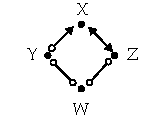
\includegraphics[width=0.3\linewidth]{fig__fci_sample_1.pdf}\label{fig:fci_samp}}
    %
    ~
    %
    \subfloat[][NOTEARS (DAG).]{\includegraphics[width=0.3\linewidth]{fig__notears_sample_1.pdf}\label{fig:notears_samp}}
    %
    ~
    %
    \subfloat[][Final ADMG.]{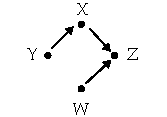
\includegraphics[width=0.3\linewidth]{fig__DAG_sample.pdf}\label{fig:dag_samp}}
    \caption{\small Resolving ties between FCI and NOTEARS.}
    \label{fig:ties}
\end{figure}

% We compare all the partially directed edges from the FCI's PAG (\fig{fci_samp_d}) with their corresponding counterparts from NOTEARS' DAG (\fig{fci_samp_e}). We experienced the following three contrasting edges between FCI and NOTEARS:
% \be[wide=0pt, topsep=0pt]
% \item \textit{\edgethree and \edgeone:} In the most common case, we observed that FCI had a partially directed edge and NOTEARS had a directed edge (as seen in the edge between \swapmem and \texttt{latency} in \Cref{fig:fci_samp_d,fig:fci_samp_e}). Here we kept the directed edge since evidence from NOTEARS provides us the directionality.
% \item  \textit{\edgefour~ and \edgeone:} In the second most common case, we observed FCI had an undirected edge and NOTEARS had a directed edge (as seen in the edge between \texttt{Resource} \texttt{Pressure} and \swapmem in \Cref{fig:fci_samp_d,fig:fci_samp_e}). Here again, we kept the directed edge in accordance with NOTEARS.
% \item \textit{\edgetwo and no edge:} Rarely, we observed that FCI had an undirected edge and NOTEARS had no edge (as seen in the edge between \gpugrowth and \swapmem in \Cref{fig:fci_samp_d,fig:fci_samp_e}). Here, we retain the bidirected edge since there likely is a latent confounder to be accommodated for.
% \ee
% %

% The final causal model would be an ADMG that resembles~\fig{fci_samp_f}. As discussed in~\tion{incremental_learning}, we update the observational data, and consequently the causal graph and the internal edge directions, periodically with new samples. %The rest of this section discusses how the causal model obtained above is used for subsequent analyses.

% \noindent\textbf{Why not use only NOTEARS?~}~We refrain from using only NOTEARS because it assumes that there are no unmeasured variables, \ie, strict causal sufficiency~\cite{lauer2017causal}. This is too restrictive since, there may be other variables that we cannot measure that may affect our observations, \eg, an increase in the environmental temperature may initiate the on-board thermal throttling fail-safe to dynamically reduce the clock speeds. FCI can accommodate such unmeasured confounders. 


% \paragraph{Phase-III: Translate Perf. Query to Causal Query}

\paragraph{Stage III: Iterative Sampling (Active Learning).}
\label{sect:path_discovery}

% In the previous stage, we convert unstructured observational data into structured ADMG. These ADMGs are still quite intricate and express several complex causal relationships among variables. 

% In this stage, we reason about the root causes of non-functional faults by: (1)~extracting the \textit{causal paths} from the ADMG and (2)~weighting the causal paths based on their average causal effect on the performance objectives. 

At this stage, \ourapproach determines the next configuration to be measured. 
\ourapproach first estimates the causal effects of configuration options towards performance objectives using the learned causal performance model. Then, \ourapproach iteratively determines the next system configuration using the estimated causal effects as a heuristic. Specifically, \ourapproach determines the value assignments for options with a probability that is determined proportionally based on their associated causal effects. The key intuition is that such changes in the options are more likely to have a larger effect on performance objectives, and therefore, we can learn more about the performance behavior of the system. Given the exponentially large configuration space and the fact that the span of performance variations is determined by a small percentage of configurations, if we had ignored such estimates for determining the change in configuration options, the next configurations would result in considerable variations in performance objectives comparing with the existing data. Therefore, measuring the next configuration would not provide additional information for the causal model. 

We extract paths from the causal graph (referred to as \textit{causal paths}) and rank them from highest to lowest based on their average causal effect on latency, and energy. Using path extraction and ranking, we reduce the complex causal graph into a few useful causal paths for further analyses. The configurations in this path are more likely to be associated with the root cause of the fault.

\noindent\textbf{Extracting causal paths with backtracking.}~A causal path is a directed path originating from either the configuration options or the system event and terminating at a non-functional property (\ie, throughput and/or energy). To discover causal paths, we backtrack from the nodes corresponding to each non-functional property until we reach a node with no parents. If any intermediate node has more than one parent, then we create a path for each parent and continue backtracking on each parent. 
% \eg, \cpufreq~\edgeone \util \edgeone Latency and  \cpucores~\edgeone \util \edgeone Latency. Since we can only intervene on configuration options we eliminate the paths that do not contain any configurations options \eg,  \contextswitches~\edgeone \cachepressure \edgeone Latency. %For example, from~\fig{fci_samp_f}, we can extract two paths:


\noindent\textbf{Ranking causal paths.~}~A complex causal graph can result in many causal paths. It is not practical to reason over all possible paths, as it may lead to a combinatorial explosion. Therefore, we rank the paths in descending of their causal effect on each non-functional property. For further analysis, we use paths with the highest causal effect.
% \label{sect:pace}
To rank the paths, we measure the causal effect of changing the value of one node (say \texttt{Batch Size} or $X$) on its successor (say \texttt{Cache Misses} or $Z$) in the path (say \texttt{Batch Size}~\edgeone \texttt{Cache Misses} \edgeone \texttt{FPS} and \texttt{Energy}). We express this with the \textit{do-calculus}~\cite{pearl2009causality} notation: $\mathbb{E}[Z~|~\mathit{do}(X=x)]$. This notation represents the expected value of $Z$ (\texttt{Cache Misses}) if we set the value of the node $X$ (\texttt{Batch Size}) to $x$. To compute the \textit{average causal effect} (ACE) of $X\rightarrow Z$ (\ie, \texttt{Batch Size} \edgeone \texttt{Cache Misses}), we find the average effect over all permissible values of $X$ (\texttt{Batch Size}), \ie, $\mathrm{ACE}\left(Z, X\right) = \frac{1}{N}\cdot \sum_{\forall a, b\in X}\mathbb{E}\left[Z~|~\mathit{do}\left(X=b\right)\right]~-~ \mathbb{E}\left[Z~|~\mathit{do}\left(X=a\right)\right]$.  Here $N$ represents the total number of values $X$ (\texttt{Batch Size}) can take. If changes in \texttt{Batch Size} result in a large change in \texttt{Cache Misses}, then $\mathrm{ACE}\left(Z, X\right)$ will be larger, indicating that \texttt{Batch Size} has a large causal effect on \texttt{Cache Misses}.

% {\footnotesize
% \begin{multline}
% \label{eq:ace}
% \mathrm{ACE}\left(Z, X\right) = \frac{1}{N}\cdot \sum_{\forall a, b\in X}\mathbb{E}\left[Z~|~\mathit{do}\left(X=b\right)\right]~-~ \mathbb{E}\left[Z~|~\mathit{do}\left(X=a\right)\right]
% \end{multline}
% }


% In this paper, we use K=3, 5,7, and 9, however, this may be modified in our replication package. 

% by carrying out the optimal intervention experiment predicted to cause the largest change in our belief (in expectation) and updating the belief. The final belief is summarized into a predicted network via Bayesian model averaging.




\paragraph{Stage IV: Update Causal Performance Model.}
\label{sect:incremental_learning}


% the estimations of causal queries act as a heuristic to select the next configuration to be measured to maximize the likelihood of improving the estimates 

At each iteration, \ourapproach measures the configuration that is determined in the previous stage and updates the causal performance model incrementally (shown in~\fig{causal_model_update}). 
Since the causal model uses limited observational data, there may be a discrepancy between the underlying performance model and the learned causal performance model, note that this issue exists in all domains using data-driven models, including causal reasoning~\cite{pearl2009causality}. The more accurate the causal graph, the more accurate the proposed intervention will be~\cite{spirtes2000causation,ogarrio2016hybrid, glymour2019review,colombo2012learning,colombo2014order}. \fig{incremental_update} (a) shows an example of an iterative decrease of hamming distance~\cite{norouzi2012hamming} between the learned causal model and (approximate) ground truth causal model. \fig{incremental_update} (b), \ref{fig:incremental_update} (c), and \ref{fig:incremental_update} (d) shows the iterative behavior of \ourapproach while debugging a multi-objective performance fault. In case our repairs do not fix the faults, we update the observational data with this new configuration and repeat the process. Over time, the estimations of causal effects will become more accurate. We terminate the incremental learning once we achieve the desired performance.

% The reason behind this initial sampling is to learn an initial causal model and given that our sampling budget is limited, we maximize the information in the causal model iteratively following a Bayesian approach where at iteration $t$ the current causal model is considered as prior and given the new sample it gets updated.



% \begin{figure}[t!]
%     % \setlength{\belowcaptionskip}{-3em}
%     \centering
%     \includegraphics*[width=\linewidth]{figures-vg/acc_shd_iter.pdf}
%     \caption{\small {}}
    
%     \label{fig:acc_shd_iter}
%     % \rayb{I have questions about this figure. Let's talk in the morning}
% \end{figure}


\paragraph{Stage V: Estimate Performance Queries.}
\label{sect:path_discovery}
At this stage, given the learned causal performance model, \ourapproach's inference engine estimates the user-specified queries using the mathematics of causal reasoning--do-calculus.
Specifically, the causal inference engine provides a quantitative estimate for the identifiable queries on the current causal model and may return some queries as unidentifiable. It also determines what assumptions or new measurements are required to answer the ``unanswerable`` questions, so, the user can decide to incorporate these new assumptions by defining more constraints or increasing the sampling budgets.

% \smallskip
% \paragraph{Implementation.}
% There are generic causal inference tools` maintained by industry (e.g., Microsoft's DoWhy~\cite{dowhy}, IBM's CausalLib~\cite{causalevaluations}, Uber's CausalML~\cite{causalml}), and academia (e.g., Ananke~\cite{ananke}, Causal Fusion~\cite{fusion}); these tools only implement the core machinery in causal reasoning including different causal modeling, structure learning, inference, counterfactuals, and estimation tasks. 
% We implemented \ourapproach by integrating and building on top of (i) \emph{Semopy}~\cite{semopy} for predictions with causal models, (ii) \emph{Ananke}~\cite{ananke} for estimating the causal effects, (iii) \emph{CausalML}~\cite{causalml} for counterfactual reasoning, \emph{PyCausal}~\cite{pycausal} for structure learning. 
% In particular, we integrated the tools into a seamless pipeline to provide users with the following capabilities for performance modeling and analyses: (i) \textbf{Modeling}: specifying the causal variables and constraints needed for learning a correct causal performance model (see Section \ref{sec:motivation}); (ii) \textbf{Analyses}: Iterative sampling, model learning and update, estimation of performance queries, and early stopping; and (iii) \textbf{User interface}: visualization, annotations, interactions with CPM models, and query estimations.

% \textcolor{blue}{To do so, we extract paths from the CPM (referred to as \textit{causal paths}) and rank them from highest to lowest based on their average causal effect (ACE) on performance objective. Using path extraction and ranking, we reduce the complex causal graph into a few useful causal paths for further analyses. The configurations in this path are more likely to be associated with the root cause of the fault.
% \noindent\textbf{Extracting causal paths with backtracking.}~A causal path is a directed path originating from either the configuration options or the system event and terminating at a non-functional property (\ie, throughput and/or energy). To discover causal paths, we backtrack from the nodes corresponding to each non-functional property until we reach a node with no parents. If any intermediate node has more than one parent, then we create a path for each parent and continue backtracking on each parent. 
% \eg, Batch Size~\edgeone Cache Misses \edgeone Throughput and En and  \cpucores~\edgeone \util \edgeone Latency. Since we can only intervene on configuration options we eliminate the paths that do not contain any configurations options \eg,  \contextswitches~\edgeone \cachepressure \edgeone Latency. %For example, from~\fig{fci_samp_f}, we can extract two paths:

% \bi[topsep=0pt] 
% \item \swapmem~\edgeone \gpugrowth \edgeone Latency; and
% \item Resource Pressure~\edgeone Latency
% \ei
% Note, there may be edges between two non-functional properties, \eg, latency\edgetwo energy. However, paths always terminate at a non-functional property, \ie, at latency, energy consumption, and heat dissipation.
% 

% \noindent\textbf{Ranking causal paths.~}~A complex causal graph can result in a large number of causal paths. It is not practical to reason over all possible paths as it may lead to a combinatorial explosion. Therefore, we rank the paths in descending of their causal effect on each non-functional property. For further analysis, we use paths with the highest causal effect.
% % \label{sect:pace}
% To rank the paths, we measure the causal effect of changing the value of one node (say \textsc{Vm Swappiness} or $X$) on its successor (say \textsc{Cache Load Misses} or $Z$) in the path (say \textsc{VM Swappiness}~\edgeone \textsc{Cache Load Misses} \edgeone \textsc{Latency} and \textsc{Energy}). We express this with the \textit{do-calculus}~\cite{pearl2009causality} notation: $\mathbb{E}[Z~|~\mathit{do}(X=x)]$. This notation represents the expected value of $Z$ (\textsc{Cache Load Misses}) if we set the value of the node $X$ (\textsc{VM Swappiness}) to $x$. To compute the \textit{average causal effect} (ACE) of $X\rightarrow Z$ (\ie, \textsc{VM Swappiness} \edgeone \textsc{Cache Load Misses}), we find the average effect over all permissible values of $X$ (\textsc{VM Swappiness}), \ie, 

% {\footnotesize
% \setlength{\abovedisplayskip}{1pt}
% \setlength{\belowdisplayskip}{1pt}
% \begin{multline}
% \label{eq:ace}
% \mathrm{ACE}\left(Z, X\right) = \frac{1}{N}\cdot \sum_{\forall a, b\in X}\mathbb{E}\left[Z~|~\mathit{do}\left(X=b\right)\right]~-~ \mathbb{E}\left[Z~|~\mathit{do}\left(X=a\right)\right]
% \end{multline}
% }

% Here, $N$ represents the total number of values $X$ (\textsc{VM Swappiness}) can take. If changes in \textsc{VM Swappiness} result in a large change in \textsc{Cache Load Misses}, then the $\mathrm{ACE}\left(Z, X\right)$ will be larger, indicating that \textsc{VM Swappiness} on average has a large causal effect on \textsc{Cache Load Misses}. %Note, if $X$ is a continuous variable, we would replace the summation of \eq{ace} with an integral. 
% % 
% % \eq{ace} represents the average causal effect over a pair of nodes in a path. 
% For the entire path, we extend \eq{ace} as:
% \smalleq
% \label{eq:path_ace}
% {\footnotesize
% \setlength{\abovedisplayskip}{1pt}
% \setlength{\belowdisplayskip}{1pt}
% \mathrm{Path}_{ACE} = \frac{1}{K} \cdot \sum \mathrm{ACE}(Z, X) \hspace{2em} \footnotesize \forall X, Z \in path 
% }
% \eeq
% \eq{path_ace} represents the average causal effect of the causal path. The configuration options that lie in paths with larger $P_{ACE}$ tend to have a greater causal effect on the corresponding non-functional properties in those paths. We select the top $K$ paths with the largest $\mathrm{P}_{ACE}$ values, for each non-functional property. In this paper, we use K=5, however, this may be modified in our replication package. 

% \noindent\textbf{\textsl{Aside.}}~In eqs.~\ref{eq:do} and~\ref{eq:ace}, $\mathbb{E}(Y~|~do(X=x))$ is \textit{not} the same as the ordinary conditional distribution $\mathbb{E}\left(Y~|~X=x\right)$. This is because $\mathbb{E}\left(Y~|~X=x\right)$ takes the original population, as is, and filters it get the sub-population where $X=x$. If $X=x$ does not exist in the population, the value of $\mathbb{E}\left(Y~|~X=x\right)$ would be misleading. In contrast, $\mathbb{E}\left(Y~|~\mathit{do}\left(X=x\right)\right)$ uses do-calculus rules~\cite{pearl2009causality} to infer the value of the distribution even when $X=x$ has never been encountered before. 

% \subsubsection{Phase-III: Counterfactual Query Evaluation}
% \label{sect:root_cause}
% Counterfactual queries can be different for different tasks. For debugging, we use the top $K$ paths to (a)~identify the root cause of non-functional faults; and (b)~prescribe ways to fix the non-functional faults.
% % \subsubsection{Translating developer's queries into counterfactual statements}
% When experiencing non-functional faults, a developer may ask specific queries to \tool and expect an actionable response. We use the example causal graph of Fig.~\ref{fig:complex} where a developer observes high latency and energy, \ie, a multi-objective fault, and has the following questions:  %We use this example to answer some of the developer's questions: 

% \noindent\textbf{\faQuestionCircle~\textbf{``What are the root causes of my multi-objective (latency and energy) fault?''}} To identify the root cause of a non-functional fault we must identify which configuration options have the most causal effect on the performance objective. %For example, in the causal graph of~\fig{path_eg}, we are required to find which of the configuration options $X_1, X_2, Z_1, Z_2$ has the highest causal effect on $Y$. 
% For this, we use the steps outlined in~\tion{path_discovery} to extract the paths from the causal graph and rank the paths based on their average causal effect (\ie, $\mathrm{Path}_{ACE}$ from \eq{path_ace}) on latency and energy. We return the configurations that lie on the top $K$ paths. 
% For example, in~\fig{fci_samp_f} we may return (say) the following paths: 
% \bisq
% \small
%     \item \textsc{VM Swappiness}~\edgeone \textsc{Cache Load Misses} \edgeone \textsc{Latency} and \textsc{Energy}
%     \item  \textsc{Scheduler Policy} \edgeone \textsc{Branch Misses} \edgeone \textsc{Cache Misses} \edgeone \textsc{Latency} and \textsc{Energy}
%     \item  \textsc{Gpu Frequency} \edgeone \textsc{Latency} and \textsc{Energy}
%     \item  \textsc{Bit Rate} \edgeone \textsc{Cache Misses} \edgeone \textsc{Latency} and \textsc{Energy}
%     \item  \textsc{Scheduler Runtime} \edgeone \textsc{Branch Misses} \edgeone \textsc{Cache Misses} \edgeone \textsc{Latency} and \textsc{Energy}
% \ei
 
% % \item \cpufreq~\edgeone \swapmem \edgeone Latency,
% and the configuration options {\textsc{VM Swappiness}, \textsc{Scheduler Policy}, \textsc{Gpu Frequency}, \textsc{Bit Rate}, \textit{and} \textsc{Scheduler Runtime}} being the probable root causes.

% \noindent\textbf{\faQuestionCircle~\textbf{``How to improve my latency and energy?''}} To answer this query, we first find the root causes as described above. Next, we discover what values each of the configuration options must take so that the new latency and energy are better (low latency and low energy) than the fault (high latency and high energy). For example, we consider the causal path \textsc{VM Swappiness}~\edgeone \textsc{Cache Load Misses} \edgeone \textsc{Latency} and \textsc{Energy}, we identify the permitted values for the configuration options {\textsc{VM Swappiness}} that can result in a low latency and energy ($Y^{\mathit{\textsc{low}}}$) that is better than the fault ($Y^{\mathit{\textsc{high}}}$).
% For this, we formulate the following counterfactual expression: 
% \smalleq
% \label{eq:cfact_bare}
% \footnotesize
% \mathrm{Pr}(Y_{repair}^{\textsc{low}}|\neg repair,Y_{\neg repair}^{\textsc{high}})
% \eeq
% \eq{cfact_bare} measures the probability of ``fixing'' the latency fault with a ``repair'' {\footnotesize $(Y_{repair}^{\textsc{low}})$} given that with no repair {we observed the fault} {\footnotesize $(Y_{\neg repair}^{\text{\textsc{high}}})$}.   
% In our example, the repairs would resemble \textsc{VM Swappiness}=$0.6$ \etc. We generate a \textit{repair set} ($\mathcal{R}_{1}$), where the configurations \textsc{VM Swappiness} is set to all permissible values, \ie,
% {
% \small
% \begin{multline}\label{eq:repairs}
%     \setlength{\abovedisplayskip}{5pt}
%     \setlength{\belowdisplayskip}{5pt}
%     \mathcal{R}_{1}\equiv~\bigcup~\left\{\textsc{VM Swappiness} = {x},... \right\}\forall {x} \in \textsc{Vm Swappiness},~\ldots
% \end{multline}}
% Observe that, in the repair set ($\mathcal{R}_{1}$) a configuration option that is not on the path \textsc{VM Swappiness}~\edgeone \textsc{Cache Load Misses} \edgeone \textsc{Latency} and \textsc{Energy} is set to the same value of the fault. For example, \textsc{Active Cores} is set to $2$ or \textsc{Gpu Frequency} is set to $0.7 \ GHz$. This way we can reason about the effect of interactions between \textsc{VM Swappiness} with other options, i.e., \textsc{Active Cores}, \textsc{Gpu Frequency}. Say \textsc{Active Cores} or \textsc{Gpu Frequency} were changed/recommended to set at any other value than the fault in some previous iteration i.e., $3$ or $1.5 \ GHz$, respectively. In that case, we set \textsc{Active Cores} and \textsc{Gpu Frequency}=$1.5 \ GHz$. Similarly, we generate a repair sets $\mathcal{R}_{2}$ to $\mathcal{R}_{5}$  by setting \textsc{Scheduler Policy}, \textsc{Gpu Frequency}, \textsc{Bit Rate} and \textsc{Scheduler Runtime} to all permissible values. 
% {
% \small
% \begin{multline}\label{eq:repairs}
%     \setlength{\abovedisplayskip}{5pt}
%     \setlength{\belowdisplayskip}{5pt}
%     \mathcal{R}_{2}\equiv~\bigcup~\left\{\textsc{Scheduler Policy} = {x},... \right\} \forall {x} \in \textsc{Scheduler Policy},~\ldots
% \end{multline}}
% {
% \small
% \begin{multline}\label{eq:repairs}
%     \setlength{\abovedisplayskip}{5pt}
%     \setlength{\belowdisplayskip}{5pt}
%     \mathcal{R}_{3}\equiv~\bigcup~\left\{\textsc{Gpu Frequency} = {x},... \right\} \forall {x} \in \textsc{Gpu Frequency},~\ldots
% \end{multline}} 
% {
% \small
% \begin{multline}\label{eq:repairs}
%     \setlength{\abovedisplayskip}{5pt}
%     \setlength{\belowdisplayskip}{5pt}
%     \mathcal{R}_{4}\equiv~\bigcup~\left\{\textsc{Bit Rate} = {x},... \right\} \forall {x} \in \textsc{Bit Rate},~\ldots
% \end{multline}} 
% {
% \small
% \begin{multline}\label{eq:repairs}
%     \setlength{\abovedisplayskip}{5pt}
%     \setlength{\belowdisplayskip}{5pt}
%     \mathcal{R}_{5}\equiv~\bigcup~\left\{\textsc{Scheduler Runtime} = {x},... \right\} \forall {x} \in \textsc{Scheduler Runtime},~\ldots
% \end{multline}} 
% Now, we combine the repair set for each path to construct a final repair set $\mathcal{R}=\mathcal{R}_{1} \cup~\ldots \cup\mathcal{R}_{k}$. Next, we compute the \textit{individual treatment effect} (ITE) on the latency and energy ($Y$) for each repair in the repair set $\mathcal{R}$. In our case, for each repair $\mathit{r}~\in~\mathcal{R}$, ITE is given by:
% \begin{equation}
%     \label{eq:ite}
%     \footnotesize
%     \mathrm{ITE}(\mathit{r})=\mathrm{Pr}(Y_r^{\textsc{low}}~|~\neg r,~Y_{\neg r}^{\textsc{high}}) - \mathrm{Pr}(Y_r^{\textsc{high}}~|~\neg r,~Y_{\neg r}^{\textsc{high}})\hspace{1em}
% \end{equation}

% % The above formulation can be extended to accommodate queries that involve multiple non-functional properties (\eg, improve \textit{both} latency and energy consumption). To do this, we may reformulate \eq{ite} to compute the probability that a repair $r$ can reduce both latency ($Y_r^{\textsc{low}}$) and the energy consumption ($W_r^{\textsc{low}}$), \ie,
% % {
% % \small
% % \begin{multline}\label{eq:repairs_2}
% %     \setlength{\abovedisplayskip}{5pt}
% %     \setlength{\belowdisplayskip}{5pt}
% %     \mathrm{ITE}(\mathit{r})=\mathrm{Pr}(Y_r^{\textsc{low}}, W_r^{\textsc{low}}~|~\neg r,~Y_{\neg r}^{\textsc{high}},~W_{\neg r}^{\textsc{high}}) \\ -~\mathrm{Pr}(Y_r^{\textsc{high}}, W_r^{\textsc{high}}~|~\neg r,~Y_{\neg r}^{\textsc{high}},~W_{\neg r}^{\textsc{high}})
% % \end{multline}}
% % \noindent\hspace{-3pt}After, computing \eq{repairs_2}, we can find a repair $r$ with the largest (positive) ITE as per~\eq{best_intervention}. 
% % \begin{equation}
% %     \label{eq:ite}
% %     \footnotesize
% %     \mathrm{ITE}(\mathit{r})=\mathrm{Pr}(Y_r^{\textsc{low}}, W_r^{\textsc{low}}~|~\neg r,~Y_{\neg r}^{\textsc{high}},~W_{\neg r}^{\textsc{high}}) - \mathrm{Pr}(Y_r^{\textsc{high}}~|~\neg r,~Y_{\neg r}^{\textsc{low}})\hspace{1em}
% % \end{equation}

% % \[\bigcup\limits_{{x_1} \in {X_1},{x_2} \in {X_2},...} {P(Y = {y_{fixed}}|do({X_1} = {x_1},{X_2} = {x_2},...))} \]

% % \noindent\textbf{\faQuestionCircle~\textbf{``How to decrease my latency using the same energy consumption''}} There queries involve multiple non-functional properties (in this case, latency and energy consumption). 
% % % An example, let us try to minimize latency without affecting energy consumption. 
% % We enumerate all possible repairs as counterfactual statements as per~\eq{repairs}. Next, we compute the \textit{individual treatment effect} (ITE) for each repair in three steps: 
% % \besq
% % \item  
% % {\footnotesize$\mathrm{P_{fix}}=\mathrm{Pr}(Y_r^\textsc{low},~W_r^\textsc{same}~|~\neg r,W_{\neg r}^\textsc{same}, Y_{\neg r}^\textsc{high} )$}.
% % \item Compute the probability that a repair $r$ \textit{cannot} fix the latency (\ie, $Y^{\text{\textsc{high}}}$) or it actually worsens energy consumption (\ie, $W^{\text{\textsc{high}}}$), \ie, {\footnotesize$\mathrm{P_{no~fix}}=\mathrm{Pr}(W_r^\textsc{high},~Y_r^\textsc{high} ~|~\neg r,W_{\neg r}^\textsc{high}, Y_{\neg r}^\textsc{high})$}.
% % \item Finally, compute the $ITE(\mathit{r})$ as {$
% % \footnotesize \mathrm{ITE}(\mathit{r})=\mathrm{P_{fix}} - \mathrm{P_{no~fix}}$}
% % \ee

% % If this difference is large, then the repair `$r$' has a high likelihood of fixing the latency fault in $Y^\text{\textsc{high}}$ while keeping the energy consumption $W^\text{\textsc{high}}$ unchanged.  We find the best repair operator with the highest $ITE(\mathit{r})$ using~\eq{best_intervention}. 

% \subsubsection*{Remarks.}~The ITE computation of \eq{ite} occurs \textit{only} on the observational data. Therefore we may generate any number of repairs and reason about them without having to deploy those interventions and measuring their performance in the real world. This offers significant runtime benefits.
% }
% If the new configuration addresses the \nfp, we return the recommended repairs to the developer. 



% We do not offer theoretical upper bounds for the convergence of the causal model. We shall address this in our future work. That said, our empirical evidence shows that our models converge after at most 50 additional samples.

% \subsection{Limitations of \tool}
% No tool is perfect, \tool is no exception. The efficacy of \tool depends on several factors such as the representativeness of the observational data or the presence of unmeasured confounders that negatively affect the quality of the causal model. An incorrect causal model may lack some crucial connections that may result in detecting spurious root causes or recommending incorrect repairs. One promising direction to address this problem would be to refine the causal model with developer feedback. Alternatively, we could transfer a causal model certified by experts for one domain to another equivalent domain. We shall explore these in future work. 

% \tool uses a query engine to translate common user queries into counterfactual statements. The query translation framework described in this section may be extended to answer more complex queries involving several more configurations and non-functional properties by reformulating the counterfactual expressions in~\eq{cfact_bare}. As part of our future work, we hope to develop a formal translation framework (\eg, in the form of a DSL) that can convert any user-provided query into a meaningful counterfactual statement. 


%%%%%% OLD %%%%%%%%
% \subsubsection{{Orienting undirected edges of the PAG from FCI}}

% We use NOTEARS \cite{zheng2018dags}, and an unconstrained optimization-based structural learning algorithm to learn a directed acyclic graph (DAG) from observational data. NOTEARS is useful for our application because it produces \textit{confidence scores} for each direction of edge orientation. We may this use to orient the partial edges. 


% Given observational data with (say) four variables $(W, X, Y, Z)$, NOTEARS learns a weighted adjacency matrix $A$. The weights determine the confidence that an edge exists between any two nodes (variables), \eg, $\left(A_{XY}=0.9, A_{YX}=0.1\right)$ indicates the confidence that there is an edge $X$\raisebox{1pt}{\edgeone}~$Y$ is 90\% while the confidence that there is an edge $Y$\raisebox{1pt}{\edgeone}~$X$ is only 10\%. 

% To generate a DAG, NOTEARS learns an adjacency matrix from the observational data. NOTEARS initializes an adjacency matrix $A$ with random values (between 0 and 1). Next, it defines a smooth function ($h$) that measures the ``DAG-ness'' of the graph such that $h(A)=0$ $\mathit{iff}$ the adjacency matrix $A$ is acyclic. Finally, it uses an unconstrained optimization to update the values of the adjacency matrix until the adjacency matrix converges. The final adjacency matrix has values that lie between 0 and 1, where 1 indicates high confidence that there is an edge and 0 otherwise.
% The directionality of the edge may be determined using the confidence scores, \eg, if $\mathit{confidence(}X$\raisebox{1pt}{\edgeone}~$Y)<\mathit{confidence}(Y$\raisebox{1pt}{\edgeone}~$X)$, then the edge directionality is $Y$\raisebox{1pt}{\edgeone}~$X$ (as seen in the edge between Resource Pressure and \swapmem in~\fig{fci_samp_e}).

% We obtain a DAG from the NOTEARS adjacency matrix to complement the PAG from FCI. This is done by setting a threshold on the confidence scores in the adjacency matrix. If the confidence of an edge in the adjacency matrix exceeds this threshold, we keep the edge otherwise we remove the edge, \eg, absent (grayed out) edge between \gpugrowth and \swapmem in~\fig{fci_samp_e}. The chosen threshold determines how many edges are retained. If the threshold is too low, then there will be a lot of spurious edges. Alternately, if the threshold is too high, the ADMG will be sparse. For this work, we found empirically that a threshold of $0.75$ for the confidence scores represented a reasonable balance. 

\section{Case Study}
\label{sec:casestudy}

\begin{figure}[tp!]
    % \setlength{\belowcaptionskip}{-3em}
    \centering
    \includegraphics*[width=\linewidth]{figures-vg/barplot_fault.pdf}
    \caption{\small {Distribution of 451 single-objective and 43 multi-objective non-functional faults across different software systems used in our study.}}
    
    \label{fig:jetson_faults}
    % \rayb{I have questions about this figure. Let's talk in the morning}
\end{figure}
Prior to a systematic evaluation in \S\ref{sec:evaluation}, here, we show how \ourapproach can enable performance debugging in a real-world scenario discussed in \cite{code_transplant:online}, where a developer migrated a real-time scene detection system from NVIDIA \txone to a more powerful hardware, \txtwo. The developer, surprisingly, experienced $4\times$ worse latency in the new environment (from 17 frames/sec in \txone to 4 frames/sec in \txtwo). % The developer expected 40\% improvement in \txtwo, \ie, 24 frames/sec. 
After two days of discussions, the performance issue was diagnosed with a misconfiguration--an incorrect setting of a compiler option and four hardware options.
Here, we assess whether and how \ourapproach could facilitate the performance debugging by comparing with (i) the fix suggested by NVIDIA in the forum, and two academic performance debugging approaches--\bugdoc~\cite{lourencco2020bugdoc} and SMAC~\cite{hutter2011sequential}.
% 


\noindent\textbf{Findings.~}~\fig{real_example} illustrates our findings. We find that:
\begin{itemize}
    \item \ourapproach could diagnose the root cause of the misconfiguration and recommends a fix within 22 minutes. Using the recommended configuration from \ourapproach, we achieved a throughput of 28 frames/sec ($65\%$ higher than \txone and $7\times$ higher than the fault). This, surprisingly, exceeds the developers' initial expectation of $30-40\%$ improvement. %(or $22-24$ FPS).
    \item \bugdoc (a diagnosis approach) has the least improvement compared to other approaches ($24\%$ improvement over \txone) while taking 4 hours to suggest the fix. \bugdoc also changed several unrelated options (depicted by \colorbox{orange!12}{\color{gray50}{\faCheck}}) not endorsed by the domain experts. 
    \item Using SMAC (an optimization approach), we aimed to find a configuration that achieves optimal throughput. However, after converging, SMAC recommended a configuration which achieved 24 frames/sec ($41\%$ better than \txone and $6\times$ better than the fault), however, could not outperform the configuration suggested by \ourapproach and even took 4 hours ($11\times$ longer than \ourapproach to converge). In addition, SMAC changed several unrelated options (\colorbox{orange!12}{\color{gray50}{\faCheck}} in~\fig{real_example}). 
\end{itemize}

  


% SMAC took 

% how cauper models this information
% what other methods miss
% what additional information can be gleaned?
\noindent\textbf{Why \ourapproach works better (and faster)?~}~%
% what the forum recommends
% This latency fault was resolved by the forum by using disabling \texttt{CUDA} \texttt{STATIC} and maximizing the clock frequencies of the CPU, GPU, and the EMC controller. This allows the software to leverage \txtwo's faster hardware. 
\ourapproach discovers the misconfigurations by constructing a causal model that rules out irrelevant configuration options and focuses on the configurations that have the highest (direct or indirect) causal effect on latency, \eg, we found the root-cause \texttt{CUDA} \texttt{STATIC} in the causal graph which indirectly affects latency via \texttt{Context Switches} (an intermediate system event). Using counterfactual queries, \ourapproach can reason about changes to configurations with the highest average causal effect (ACE) (last column in~\fig{real_example}). The counterfactual reasoning occurs no additional measurements, significantly speeding up inference as shown in \fig{real_example}, \ourapproach accurately finds all the configuration options recommended by the forum (depicted by \colorbox{blue!10}{\color{gray50}{\faCheck}} in~\fig{real_example}).

% Together, the causal model and the counterfactual reasoning enable \tool to pinpoint the configuration options that were misconfigured and recommend a fix for them promptly. A Further, \tool recommends fixes to these options that result in $24\%$ better latency than the recommendation by domain experts in the forum. More importantly, \tool takes only 24 minutes (vs. 2 days of forum discussion) without modifying unrelated configurations. 
% 
% \subsubsection*{Aside.}~In several cases, especially with network performance faults, developers on the forum often manually inspect trace logs obtained by utilities such as \texttt{iperf} to understand the possible bottlenecks~\cite{HighCPUu7:online}. These traces contain a large volume of information about the current state of the system (\eg, network load, \, etc). Sifting through this log to decipher the source of faults is very cumbersome taking months to resolve in some cases.  

% In the rest of the paper, we perform a detailed evaluation \tool on 
% Without causal models, 
% \subsubsection*{Limitations of other methods.~}~%
% \bisq
% \item [$circ$] 
% \item[$\circ$] \textit{Inference time:} SMAC takes up to 4 hours to generate an near-optimal configuration. SMAC explores the configuration space to find a near-optimal. Due to the complexity of the configuration space, SMAC is forced to explore and evaluate several sub-optimal configurations. 
% \ei
\input{5_evaluation.tex}
\section{Evaluation}
\label{sec:evaluation}
\begin{table}[tb!]
\caption{Overview of the subject systems used in our study. Details about the configuration options and system events for each system are found in the \href{https://github.com/softsys4ai/unicorn}{\color{blue!80}supplementary materials}.}
\label{tab:subject_systems}
\resizebox{0.98\linewidth}{!}{%
\begin{tabular}{@{}lp{4cm}llllll@{}}

\toprule
System      & Workload     & $|\mathcal{C}|$ & $|\mathcal{O}|$ & $|\mathcal{S}|$ & $|\mathcal{H}|$ & $|\mathcal{W}|$ & $|\mathcal{P}|$  \\ \midrule
\textsc{Deepstream}~\cite{DeepStream} & Video analytics pipeline for detection and tracking from 8 camera streams. & 2461    & 53 & 288  & 2  & 1 & 2 \\
                    
                     

\textsc{Xception}~\cite{chollet2017xception}   & Image recognition system to classify 5000/5000 test images from CIFAR10. & 6443  & 28 & 19  & 3  & 3 & 3 \\
                    
                    

\textsc{Deepspeech}~\cite{hannun2014deep} &Speech-to-text from 0.5/1932 hours of Common Voice Corpus 5.1 (English) data.      & 6112  & 28 & 19  & 3  & 1 & 3 \\
 


\textsc{Bert}~\cite{devlin2018bert}       & NLP system for sentiment analysis of 1000/25000 test reviews from IMDb.           & 6188  & 28 & 19  & 3  & 1 & 3 \\
  

\textsc{x264}~\cite{x264}       & Encodes a 20 second 11.2 MB video of resolution 1920 x 1080 from UGC.  & 17248  & 32 & 19  & 3  & 1 & 3 \\


\textsc{SQLite}~\cite{SQLite}     & Database engine for sequential \& batch \& random reads, writes, deletions.     & 15680   & 242 & 288  & 3  & 3 & 3 \\

\bottomrule
\end{tabular}}
{* \tiny $\mathcal{C}$: Configurations, $\mathcal{O}$: Options, $\mathcal{S}$: System Events, $\mathcal{H}$: Hardware, $\mathcal{W}$: Workload, $\mathcal{P}$: Objectives}
\vspace{-4mm}
\end{table}

For a thorough evaluation of \ourapproach, we have developed \ourtool that implements the methodology that we explained in \S\ref{sec:methodology}.
We used \ourtool (see \S\ref{sec:artifact}) to facilitate comparing \ourapproach with state-of-the-art performance debugging and optimization approaches for: 
\begin{itemize}
\item \textbf{Effectiveness} in terms of sample efficiency and performance gain (\S\ref{sec:effectiveness}).
\item \textbf{Transferability} of learned models across environmental changes such as hardware and workload changes (\S\ref{sec:transfer}).
\item \textbf{Scalability} to large-scale configurable systems (\S\ref{sec:scalability}).
\end{itemize}

% \begin{itemize}[leftmargin=*,itemsep=0pt,labelsep=5pt]
% \item \textbf{RQ1: Effectiveness.} evaluate
% \item \textbf{RQ2: Sample Efficiency.} How sample efficient is \tool for different performance tasks?
% \item \textbf{RQ2: Transferrability.} How transferrable is \tool for different performance tasks?
% \item \textbf{RQ4: Scalability.} How scalable is \tool for growing configuration spaces for different performance tasks?
% \end{itemize}


% \subsection{Setting}
% This section describes our experimental setup to demonstrate the strength of \tool for performance tasks in multiple hardware and workloads. 
%Due to space constraints, we limit our scope to performance debugging and performance optimization.


%\subsection{Systems}
\noindent
\textbf{Systems.} We selected six configurable systems including a video analytic pipeline, three deep learning-based systems (for image, speech, and NLP), a video encoder, and a database, see Table~\ref{tab:subject_systems}. We use heterogeneous deployment platforms, including \textsc{NVIDIA} \txone, \txtwo, and \xavier, each having different resources (compute, memory) and microarchitectures. 

% Each platform has different hardware specifications, \eg, different CPU micro-architectures (ARM Caramel, Cortex), GPU micro-architectures (Maxwell, Pascal, Volta), energy requirements (5W--30W).

% This software has different functionalities and configuration complexities (ranging from 28 to 242 configuration options) as shown in Table~\ref{tab:subject_systems}.  
%\textsc{Deepstream} is an end-to-end video analytics pipeline of a composed system that is used to track detected objects from multiple camera streams (discussed details earlier). \textsc{Xception} is a CNN based Image recognition software that is used for classification of 5000 testing images from the \textsc{CIFAR10} dataset~\cite{chollet2017xception}. \textsc{Deepspeech} is an RNN based speech recognition system to recognize voices from randomly extracted 30 minutes of English language voice data for English languages from 1932 hours of voice data of the Common Voice Corpus5.1~\cite{hannun2014deep} with chunks of 5 seconds each. NLP software \textsc{BERT} performs sentiment analysis on 1000 reviews randomly extracted from the 25000 testing example provided in the IMDb dataset~\cite{devlin2018bert}. \textsc{x264} is used to encode a 20-second long video file of 11.2 MB with resolution 1920 x 1080 selected from the UGC dataset. \textsc{sqlite} is a database management system used to perform a different number of sequential reads, random reads, sequential writes, batch writes, and delete operations. 

% \noindent\textbf{Hardware.} To deploy these software systems, we use three NVIDIA Jetson Platforms: \txone, \txtwo, and \xavier. Each platform has different hardware specifications, \eg, different CPU micro-architectures (ARM Caramel, Cortex), GPU micro-architectures (Maxwell, Pascal, Volta), energy requirements (5W--30W). 

\noindent\textbf{Configurations.} We choose a wide range of configuration options and system events (see Table~\ref{tab:subject_systems}), following \textsc{NVIDIA}'s configuration guides/tutorials and other related work~\cite{Halawa2017}. As opposed to prior works (e.g.,~\cite{velez2021white,VJSSAK:ASE20}) that only support binary options due to scalability issues, we included options with binary, discrete, and continuous.

% For continuous options, we choose 10 equally spaced values between the minimum and maximum permissible values, \eg, for \gpugrowth, we vary the value between 0\% and 100\% in steps of 10\%. For non-binary options with two different values, we encode the values as a binary option. 

% \noindent
% \textbf{Ground truth data.} %For collecting the ground truths, we estimate the performance of the systems by setting the configurations in different permissible values. In particular, we measure the throughput and energy for \textsc{Deepstream}, and latency, energy, and heat for the remaining five software systems. 
% As the configuration space of the systems is intractably large, we randomly select configurations by setting an experimental budget of 3 days per system. We repeat each measurement $5$ times and record the median to reduce the effect of measurement noise and other variabilities~\cite{iqbal2019transfer}. Thus, for six software systems on three hardware platforms, it took two months of computing time to collect all these data for experimental evaluation. We set the seed value to 88 to reproduce our work.

\noindent \textbf{Ground truth.} We measured several thousands samples (proportional to the configuration space of the system, see \href{https://github.com/softsys4ai/unicorn}{\color{blue!80}supplementary materials} for specific dataset size) for each 18 deployment settings (6 systems and 3 hardware; see Table \ref{tab:subject_systems} for more details). To ensure reliable and replicable results, following the common practice~\cite{ding2021generalizable,JSVKPA:ASE17,curtsinger2013stabilizer,kaltenecker2020interplay}, we repeated each measurement $5$ times and used the median in the evaluation metrics. 
We curated a ground truth of performance issues, called {\sc Jetson Faults}, for each of the studied software and hardware systems using the ground truth data. By definition, non-functional faults are located in the tail of performance distributions~\cite{gunawi2018fail,kleppmann2017designing}. We, therefore, selected and labeled configurations that are worse than the $99^\text{th}$ percentile as `\textit{faulty}.' ~\fig{jetson_faults} shows the total 494 faults discovered across different software. Out of these 494 non-functional faults, 43 are faults with multiple types (both energy and latency). Of all the 451 single-objective and 43 multi-objective faults discovered in this study, only 2 faults had a single root cause, 411 faults had five or more root causes, and 81 remaining faults had two to four root causes. 

\noindent \textbf{Experimental parameters}. To facilitate replication of the results, we made some choices for specific parameters. In particular, we disabled dynamic voltage and frequency scaling (DVFS) before starting any experiment and start with 25 samples for each method~(10\% of the total sampling budget). We repeat the entire process 3 times for consistent analyses.


% We created a ground truth for \textit{fixes} by inspecting each configuration labeled faulty and identifying their root causes manually. We manually reconfigure each incorrect configuration to achieve the best possible latency and energy and thereby dispensing with the nf-faults. For single-objective \textsc{nf-faults}, we manually select the configuration with maximum gain as the ground truth. For multi-objective \textsc{nf-faults}, we select the Pareto-optimal configurations as the ground truth. For each reconfiguration, we record the changed configuration options and the values; these are used as a reference for evaluation. Of all the 451 single-objective and 43 multi-objective \textsc{nf-faults} discovered in this study, only 2 faults (less than 1\%) had a single configuration option as the root cause, 411 faults (83\%) had five or more options as the root causes and remaining 81 faults (16\%) had two to four options as the root causes. 




% \item \textbf{Task 1.}~Determining configurations to resolve non-functional faults resulting due to misconfigurations, and 


% \begin{table*}[t!]
% \centering
% \caption{\small (RQ1) Efficiency of \bfseries\tool compared to default and statistical debugging approaches. Cells highlighted in \colorbox[HTML]{C9E7BF}\bfseries{green} highlight better performance. \bfseries\tool achieves better performance overall.}
% \label{tab:rq1_1}
% \resizebox{\textwidth}{!}{
% \begin{tabular}{@{}l|l|rrrrrrrrr|rrr|rrr|rrr|rrr|rrr|rrr|@{}}
%  \multicolumn{1}{c}{}&  & \multicolumn{9}{c|}{TX1} & \multicolumn{9}{c|}{TX2} & \multicolumn{9}{c|}{Xavier} \bigstrut\\ \clineB{3-29}{2}
%  \multicolumn{1}{c}{}&  & \multicolumn{3}{c|}{Accuracy} & \multicolumn{3}{c|}{Recall} & \multicolumn{3}{c|}{Precision} & \multicolumn{3}{c|}{Accuracy} & \multicolumn{3}{c|}{Recall} & \multicolumn{3}{c|}{Precision} & \multicolumn{3}{c|}{Accuracy} & \multicolumn{3}{c|}{Recall} & \multicolumn{3}{c|}{Precision} \bigstrut\\ \clineB{3-29}{2}
% \multicolumn{1}{c}{\multirow{-3}{*}{}} & \multicolumn{1}{c|}{\multirow{-3}{*}{Software}} & \multicolumn{1}{r}{\rotatebox{90}{\bfseries\tool}} & \multicolumn{1}{r}{\rotatebox{90}{CBI~\cite{song2014statistical}~}} & \multicolumn{1}{r|}{\rotatebox{90}{Default}} & \multicolumn{1}{r}{\rotatebox{90}{\bfseries\tool}} & \multicolumn{1}{r}{\rotatebox{90}{CBI~\cite{song2014statistical}~}} & \multicolumn{1}{r|}{\rotatebox{90}{Default}} & \multicolumn{1}{r}{\rotatebox{90}{\bfseries\tool}} & \multicolumn{1}{r}{\rotatebox{90}{CBI~\cite{song2014statistical}~}} & \multicolumn{1}{r|}{\rotatebox{90}{Default}} & \multicolumn{1}{r}{\rotatebox{90}{\bfseries\tool}} & \multicolumn{1}{r}{\rotatebox{90}{CBI~\cite{song2014statistical}~}} & \multicolumn{1}{r|}{\rotatebox{90}{Default}} & \multicolumn{1}{r}{\rotatebox{90}{\bfseries\tool}} & \multicolumn{1}{r}{\rotatebox{90}{CBI~\cite{song2014statistical}~}} & \multicolumn{1}{r|}{\rotatebox{90}{Default}} & \multicolumn{1}{r}{\rotatebox{90}{\bfseries\tool}} & \multicolumn{1}{r}{\rotatebox{90}{CBI~\cite{song2014statistical}~}} & \multicolumn{1}{r|}{\rotatebox{90}{Default}} & \multicolumn{1}{r}{\rotatebox{90}{\bfseries\tool}} & \multicolumn{1}{r}{\rotatebox{90}{CBI~\cite{song2014statistical}~}} & \multicolumn{1}{r|}{\rotatebox{90}{Default}} & \multicolumn{1}{r}{\rotatebox{90}{\bfseries\tool}} & \multicolumn{1}{r}{\rotatebox{90}{CBI~\cite{song2014statistical}~}} & \multicolumn{1}{r|}{\rotatebox{90}{Default}} & \multicolumn{1}{r}{\rotatebox{90}{\bfseries\tool}} & \multicolumn{1}{r}{\rotatebox{90}{CBI~\cite{song2014statistical}~}} & \multicolumn{1}{r|}{\rotatebox{90}{Default}} \bigstrut\\ \hlineB{2}B{2}
%  & DNN Image & \cellcolor{blue!10}\bfseries84 & 75 & \multicolumn{1}{r|}{59} & \cellcolor{blue!10}\bfseries81 & 67 & \multicolumn{1}{r|}{64} & \cellcolor{blue!10}\bfseries88 & 79 & 50 & \cellcolor{blue!10}\bfseries88 & 57 & 52 & \cellcolor{blue!10}\bfseries86 & 62 & 70 & \cellcolor{blue!10}\bfseries91 & 53 & 46 & \cellcolor{blue!10}\bfseries74 & 68 & 67 & \cellcolor{blue!10}\bfseries79 & 62 & 57 & \cellcolor{blue!10}\bfseries72 & 72 & 69 \bigstrut\\
%  & DNN Speech & \cellcolor{blue!10}\bfseries88 & 76 & \multicolumn{1}{r|}{61} & \cellcolor{blue!10}\bfseries83 & 70 & \multicolumn{1}{r|}{70} & \cellcolor{blue!10}\bfseries94 & 80 & 58 & \cellcolor{blue!10}\bfseries76 & 61 & 55 & \cellcolor{blue!10}\bfseries75 & 65 & 57 & \cellcolor{blue!10}\bfseries81 & 57 & 45 & \cellcolor{blue!10}\bfseries78 & 64 & 63 & \cellcolor{blue!10}\bfseries81 & 62 & 60 & \cellcolor{blue!10}\bfseries79 & 71 & 69 \bigstrut\\
%  & DNN NLP & \cellcolor{blue!10}\bfseries90 & 78 & \multicolumn{1}{r|}{59} & \cellcolor{blue!10}\bfseries74 & 70 & \multicolumn{1}{r|}{61} & \cellcolor{blue!10}\bfseries92 & 82 & 56 & 64 & \cellcolor{blue!10}\bfseries68 & 45 & 62 & \cellcolor{blue!10}\bfseries69 & 56 & \cellcolor{blue!10}\bfseries74 & 57 & 49 & \cellcolor{blue!10}\bfseries84 & 70 & 69 & \cellcolor{blue!10}\bfseries80 & 63 & 54 & \cellcolor{blue!10}\bfseries86 & 69 & 71 \bigstrut\\
%  & x264 & \cellcolor{blue!10}\bfseries92 & 77 & \multicolumn{1}{r|}{58} & \cellcolor{blue!10}\bfseries79 & 75 & \multicolumn{1}{r|}{67} & \cellcolor{blue!10}\bfseries96 & 82 & 59 & \cellcolor{blue!10}\bfseries83 & 68 & 47 & \cellcolor{blue!10}\bfseries82 & 55 & 70 & \cellcolor{blue!10}\bfseries85 & 53 & 58 & \cellcolor{blue!10}\bfseries84 & 68 & 63 & \cellcolor{blue!10}\bfseries75 & 63 & 56 & \cellcolor{blue!10}\bfseries83 & 69 & 71 \bigstrut\\
% \multirow{-5}{*}{\rotatebox{90}{Latency}} & SQLite & \cellcolor{blue!10}\bfseries87 & 75 & \multicolumn{1}{r|}{65} & \cellcolor{blue!10}\bfseries82 & 74 & \multicolumn{1}{r|}{63} & \cellcolor{blue!10}\bfseries91 & 81 & 61 & \cellcolor{blue!10}\bfseries80 & 62 & 59 & \cellcolor{blue!10}\bfseries78 & 59 & 68 & \cellcolor{blue!10}\bfseries84 & 51 & 52 & \cellcolor{blue!10}\bfseries83 & 65 & 70 & \cellcolor{blue!10}\bfseries79 & 62 & 56 & \cellcolor{blue!10}\bfseries76 & 69 & 70 \bigstrut\\ \hlineB{2}B{2}
%  & DNN Image & \cellcolor{blue!10}\bfseries77 & 61 & \multicolumn{1}{r|}{27} & \cellcolor{blue!10}\bfseries74 & 58 & \multicolumn{1}{r|}{62} & \cellcolor{blue!10}\bfseries74 & 66 & 21 & \cellcolor{blue!10}\bfseries84 & 61 & 53 & \cellcolor{blue!10}\bfseries86 & 63 & 48 & \cellcolor{blue!10}\bfseries78 & 50 & 51 & \cellcolor{blue!10}\bfseries70 & 61 & 50 & \cellcolor{blue!10}\bfseries78 & 62 & 48 & \cellcolor{blue!10}\bfseries67 & 57 & 56 \bigstrut\\
%  & DNN Speech & \cellcolor{blue!10}\bfseries76 & 62 & \multicolumn{1}{r|}{25} & \cellcolor{blue!10}\bfseries72 & 63 & \multicolumn{1}{r|}{58} & \cellcolor{blue!10}\bfseries72 & 65 & 26 & \cellcolor{blue!10}\bfseries77 & 61 & 50 & \cellcolor{blue!10}\bfseries80 & 63 & 53 & \cellcolor{blue!10}\bfseries74 & 54 & 49 & \cellcolor{blue!10}\bfseries75 & 56 & 50 & \cellcolor{blue!10}\bfseries79 & 62 & 41 & \cellcolor{blue!10}\bfseries65 & 56 & 55 \bigstrut\\
%  & DNN NLP & \cellcolor{blue!10}\bfseries74 & 60 & \multicolumn{1}{r|}{19} & \cellcolor{blue!10}\bfseries68 & 59 & \multicolumn{1}{r|}{64} & \cellcolor{blue!10}\bfseries73 & 66 & 20 & \cellcolor{blue!10}\bfseries73 & 65 & 57 & \cellcolor{blue!10}\bfseries70 & 63 & 45 & \cellcolor{blue!10}\bfseries77 & 52 & 43 & \cellcolor{blue!10}\bfseries77 & 59 & 49 & \cellcolor{blue!10}\bfseries77 & 63 & 40 & \cellcolor{blue!10}\bfseries83 & 57 & 53 \bigstrut\\
%  & x264 & \cellcolor{blue!10}\bfseries65 & 64 & \multicolumn{1}{r|}{27} & \cellcolor{blue!10}\bfseries69 & 64 & \multicolumn{1}{r|}{56} & \cellcolor{blue!10}\bfseries73 & 66 & 27 & \cellcolor{blue!10}\bfseries79 & 66 & 54 & \cellcolor{blue!10}\bfseries77 & 63 & 46 & \cellcolor{blue!10}\bfseries83 & 44 & 42 & \cellcolor{blue!10}\bfseries79 & 56 & 51 & \cellcolor{blue!10}\bfseries72 & 63 & 45 & \cellcolor{blue!10}\bfseries80 & 59 & 50 \bigstrut\\
% \multirow{-5}{*}{\rotatebox{90}{Energy}} & SQLite & \cellcolor{blue!10}\bfseries79 & 57 & \multicolumn{1}{r|}{24} & \cellcolor{blue!10}\bfseries69 & 58 & \multicolumn{1}{r|}{52} & \cellcolor{blue!10}\bfseries70 & 69 & 32 & \cellcolor{blue!10}\bfseries82 & 67 & 45 & \cellcolor{blue!10}\bfseries70 & 61 & 48 & \cellcolor{blue!10}\bfseries81 & 45 & 47 & \cellcolor{blue!10}\bfseries78 & 58 & 51 & \cellcolor{blue!10}\bfseries78 & 62 & 42 & \cellcolor{blue!10}\bfseries80 & 60 & 51 \bigstrut\\ \hlineB{2}B{2}
%  & DNN Image & \cellcolor{blue!10}\bfseries65 & 63 & \multicolumn{1}{r|}{53} & \cellcolor{blue!10}\bfseries80 & 65 & \multicolumn{1}{r|}{69} & \cellcolor{blue!10}\bfseries64 & 55 & 58 & \cellcolor{blue!10}\bfseries72 & 65 & 59 & \cellcolor{blue!10}\bfseries73 & 57 & 52 & \cellcolor{blue!10}\bfseries64 & 58 & 54 & \cellcolor{blue!10}\bfseries67 & 58 &52 & \cellcolor{blue!10}\bfseries72 & \cellcolor{blue!10}\bfseries72 & 56 & \cellcolor{blue!10}\bfseries53 & 51 & 49 \bigstrut\\
%  & DNN Speech & \cellcolor{blue!10}\bfseries69 & 61 & \multicolumn{1}{r|}{55} & \cellcolor{blue!10}\bfseries76 & 68 & \multicolumn{1}{r|}{69} & \cellcolor{blue!10}\bfseries69 & 57 & 52 & \cellcolor{blue!10}\bfseries67 & 57 & 47 & \cellcolor{blue!10}\bfseries66 & 65 & 66 & \cellcolor{blue!10}\bfseries67 & 56 & 60 & \cellcolor{blue!10}\bfseries68 & 54 & 64 & \cellcolor{blue!10}\bfseries74 & 69 & 60 & \cellcolor{blue!10}\bfseries68 & 57 & 48 \bigstrut\\
%  & DNN NLP & \cellcolor{blue!10}\bfseries66 & 53 & \multicolumn{1}{r|}{57} & \cellcolor{blue!10}\bfseries81 & 65 & \multicolumn{1}{r|}{69} & \cellcolor{blue!10}\bfseries63 & 59 & 53 & \cellcolor{blue!10}\bfseries57 & 52 & 59 & \cellcolor{blue!10}\bfseries58 & 57 & 56 & \cellcolor{blue!10}\bfseries53 & 51 & 52 & \cellcolor{blue!10}\bfseries66 & 55 & 58 & \cellcolor{blue!10}\bfseries79 & 57 & 58 & \cellcolor{blue!10}\bfseries54 & 52 & 48 \bigstrut\\
%  & x264 & \cellcolor{blue!10}\bfseries68 & 62 & \multicolumn{1}{r|}{51} & \cellcolor{blue!10}\bfseries76 & 75 & \multicolumn{1}{r|}{73} & \cellcolor{blue!10}\bfseries66 & 51 & 54 & \cellcolor{blue!10}\bfseries64 & 65 & 60 & \cellcolor{blue!10}\bfseries64 & 56 & 68 & \cellcolor{blue!10}\bfseries58 & 51 & 56 & \cellcolor{blue!10}\bfseries70 & 66 & 66 & \cellcolor{blue!10}\bfseries77 & 66 & 60 & \cellcolor{blue!10}\bfseries58 & 52 & 48 \bigstrut\\
% \multirow{-5}{*}{\rotatebox{90}{Thermals}} & SQLite & \cellcolor{blue!10}\bfseries70 & 53 & \multicolumn{1}{r|}{54} & \cellcolor{blue!10}\bfseries75 & 65 & \multicolumn{1}{r|}{70} & \cellcolor{blue!10}\bfseries66 & 50 & 48 & \cellcolor{blue!10}\bfseries65 & 68 & 60 & \cellcolor{blue!10}\bfseries73 & 60 & 57 & \cellcolor{blue!10}\bfseries63 & 58 & 54 & \cellcolor{blue!10}\bfseries73 & 62 & 58 & \cellcolor{blue!10}\bfseries78 & 57 & 50 & \cellcolor{blue!10}\bfseries62 & 65 & 46 \bigstrut\\ \hlineB{2}B{2}
% \end{tabular}
% }
% \end{table*}

% \begin{table*}[]
%     \centering
%     \caption{\small  Efficiency of \tool compared to other approaches. Cells highlighted in \colorbox{blue!10}{\bfseries blue} indicate improvement over faults and \colorbox[HTML]{FFCCC9}{red} indicate deterioration. Overall,\tool achieves better performance overall and is much faster.
%     }
% \vspace{-0.85em}
% \subfloat[Single objective performance fault in latency, energy consumption, or thermal dissipation.]{\scriptsize
%     \label{tab:rq1_1}
%     \resizebox{0.85\textwidth}{!}{
%     \begin{tabular}{@{}l|l|l|lllll|lllll|lllll|lllll|ll|}
%         \clineB{4-25}{2}
%         \multicolumn{1}{c}{}&\multicolumn{1}{c}{}  &  & \multicolumn{5}{c|}{Accuracy} & \multicolumn{5}{c|}{Precision} & \multicolumn{5}{c|}{Recall} & \multicolumn{5}{c|}{Gain} & \multicolumn{2}{c|}{Time$^\dagger$} \bigstrut\\ \clineB{4-25}{2}
%         \multicolumn{1}{c}{}& \multicolumn{1}{c}{} &  & \multicolumn{1}{c}{\rotatebox{90}{\bfseries\tool}} & \multicolumn{1}{c}{\rotatebox{90}{\cbi}} & \multicolumn{1}{c}{\rotatebox{90}{\dd}} & \multicolumn{1}{c}{\rotatebox{90}{\encore}} & \multicolumn{1}{c|}{\rotatebox{90}{\bugdoc~}} & \multicolumn{1}{c}{\rotatebox{90}{\bfseries\tool}} & \multicolumn{1}{c}{\rotatebox{90}{\cbi}} & \multicolumn{1}{c}{\rotatebox{90}{\dd}} & \multicolumn{1}{c}{\rotatebox{90}{\encore}} & \multicolumn{1}{c|}{\rotatebox{90}{\bugdoc~}} & \multicolumn{1}{c}{\rotatebox{90}{\bfseries\tool}} & \multicolumn{1}{c}{\rotatebox{90}{\cbi}} & \multicolumn{1}{c}{\rotatebox{90}{\dd}} & \multicolumn{1}{c}{\rotatebox{90}{\encore}} & \multicolumn{1}{c|}{\rotatebox{90}{\bugdoc~}} & \multicolumn{1}{c}{\rotatebox{90}{\bfseries\tool}} & \multicolumn{1}{c}{\rotatebox{90}{\cbi}} & \multicolumn{1}{c}{\rotatebox{90}{\dd}} & \multicolumn{1}{c}{\rotatebox{90}{\encore}} & \multicolumn{1}{c|}{\rotatebox{90}{\bugdoc~}} & \multicolumn{1}{c}{\rotatebox{90}{\bfseries\tool}} & \multicolumn{1}{c|}{\rotatebox{90}{Others}} \bigstrut[t]
%         \\ \clineB{4-25}{2}
%     \multicolumn{1}{c}{}&\multicolumn{1}{c}{}  & \multicolumn{1}{c}{} & \multicolumn{1}{c}{} & \multicolumn{1}{c}{} & \multicolumn{1}{c}{} & \multicolumn{1}{c}{} & \multicolumn{1}{c}{} \bigstrut\\[-1.4em]\hlineB{2}
%      &  & Image & \cellcolor{blue!10}\bfseries84 & 66 & 65 & 68 & 71 & \cellcolor{blue!10}\bfseries 84 & 67 & 61 & 63 & 67 & \cellcolor{blue!10}\bfseries80 & 64 & 68 & 69 & 62 & \cellcolor{blue!10}\bfseries81 & 48 & 42 & 57 & 59 & \cellcolor{blue!10}\bfseries0.6 & 4 \\
%      &  & NLP & \cellcolor{blue!10}\bfseries76 & 65 & 60 & 66 & 66 & \cellcolor{blue!10}\bfseries77 & 57 & 55 & 61 & 73 & \cellcolor{blue!10}\bfseries 66 & 74 & 68 & 67 & 65 & \cellcolor{blue!10}\bfseries74 & 54 & 59 & 62 & 58 & \cellcolor{blue!10}\bfseries0.2 & 4 \\
%      &  & Speech & \cellcolor{blue!10}\bfseries75 & 64 & 63 & 63 & 72 & \cellcolor{blue!10}\bfseries71 & 58 & 69 & 61 & 68 & \cellcolor{blue!10}\bfseries79 & 73 & 61 & 63 & 69 & \cellcolor{blue!10}\bfseries77 & 59 & 53 & 55 & 66 & \cellcolor{blue!10}\bfseries0.7 & 4 \\
%      &  & x264 & \cellcolor{blue!10}\bfseries76 & 67 & 60 & 61 & 70 & \cellcolor{blue!10}\bfseries74 & 69 & 58 & 65 & 66 & \cellcolor{blue!10}\bfseries77 & 64 & 67 & 23 & 72 & \cellcolor{blue!10}\bfseries23 & 9 & 12 & 8 & 11 & \cellcolor{blue!10}\bfseries1.2 & 4 \\
%     \multirow{-5}{*}{\rotatebox{90}{\txtwo}} & \multirow{-5}{*}{\rotatebox{90}{Latency}} & SQLite & \cellcolor{blue!10}\bfseries84 & 65 & 68 & 65 & 70 & \cellcolor{blue!10}\bfseries70 & 61 & 62 & 70 & 70 & \cellcolor{blue!10}\bfseries84 & 69 & 69 & 64 & 69 & \cellcolor{blue!10}\bfseries 19 & 13 & 11 & 12 & 8 & \cellcolor{blue!10}\bfseries0.5 & 4 \\ \hlineB{2}
%     \multicolumn{1}{c}{}&\multicolumn{1}{c}{}  & \multicolumn{1}{c}{} & \multicolumn{1}{c}{} & \multicolumn{1}{c}{} & \multicolumn{1}{c}{} & \multicolumn{1}{c}{} & \multicolumn{1}{c}{} \bigstrut\\[-1.55em]\hlineB{2}
    
%      &  & Image & \cellcolor{blue!10}\bfseries74 & 63 & 55 & 63 & 64 & \cellcolor{blue!10}\bfseries73 & 56 & 58 & 66 & 65 & \cellcolor{blue!10}\bfseries80 & 69 & 55 & 63 & 68 & \cellcolor{blue!10}\bfseries83 & 59 & 50 & 35 & 51 & \cellcolor{blue!10}\bfseries0.2 & 4 \\
%      &  & NLP & \cellcolor{blue!10}\bfseries77 & 60 & 63 & 66 & 64 & \cellcolor{blue!10}\bfseries71 & 62 & 64 & 64 & 65 & \cellcolor{blue!10}\bfseries66 & 61 & 54 & 63 & 66 & \cellcolor{blue!10}\bfseries63 & 49 & 36 & 49 & 53 & \cellcolor{blue!10}\bfseries0.4 & 4 \\
%      &  & Speech & \cellcolor{blue!10}\bfseries73 & 66 & 65 & 61 & 71 & \cellcolor{blue!10}\bfseries75 & 55 & 59 & 54 & 68 & \cellcolor{blue!10}\bfseries79 & 53 & 52 & 59 & 71 & \cellcolor{blue!10}\bfseries82 & 64 & 48 & 65 & 63 & \cellcolor{blue!10}\bfseries1.1 & 4 \\
%      &  & x264 & \cellcolor{blue!10}\bfseries74 & 62 & 57 & 59 & 67 & \cellcolor{blue!10}\bfseries81 & 63 & 53 & 61 & 66 & \cellcolor{blue!10}\bfseries77 & 67 & 53 & 54 & 72 & \cellcolor{blue!10}\bfseries26 & 13 & 11 & 16 & 16 & \cellcolor{blue!10}\bfseries0.1 & 4 \\
%     \multirow{-5}{*}{\rotatebox{90}{\xavier}} & \multirow{-5}{*}{\rotatebox{90}{Energy}} & SQLite & \cellcolor{blue!10}\bfseries80 & 53 & 62 & 66 & 71 & \cellcolor{blue!10}\bfseries80 & 52 & 66 & 64 & 72 & \cellcolor{blue!10}\bfseries84 & 53 & 67 & 65 & 69 & \cellcolor{blue!10}\bfseries21 & 16 & 10 & 14 & 15 & \cellcolor{blue!10}\bfseries0.5 & 4 \\ \hlineB{2}
%     \multicolumn{1}{c}{}&\multicolumn{1}{c}{}  & \multicolumn{1}{c}{} & \multicolumn{1}{c}{} & \multicolumn{1}{c}{} & \multicolumn{1}{c}{} & \multicolumn{1}{c}{} & \multicolumn{1}{c}{} \bigstrut\\[-1.55em]\hlineB{2}
    
%      &  & Image & \cellcolor{blue!10}\bfseries69 & 63 & 57 & 64 & 65 & \cellcolor{blue!10}\bfseries75 & 56 & 56 & 60 & 66 & \cellcolor{blue!10}\bfseries68 & 70 & 58 & 64 & 62 & \cellcolor{blue!10}\bfseries3 & 3 & 2 & 2 & 2 & \cellcolor{blue!10}\bfseries0.7 & 4 \\
%      &  & NLP & \cellcolor{blue!10}\bfseries71 & 62 & 61 & 61 & 62 & \cellcolor{blue!10}\bfseries72 & 56 & 59 & 56 & 61 & \cellcolor{blue!10}\bfseries72 & 65 & 62 & 67 & 62 & \cellcolor{blue!10}\bfseries5 & 4 & 1 & 2 & 4 & \cellcolor{blue!10}\bfseries0.4 & 4 \\
%      &  & Speech & \cellcolor{blue!10}\bfseries71 & 61 & 64 & 62 & 67 & \cellcolor{blue!10}\bfseries71 & 58 & 59 & 54 & 68 & \cellcolor{blue!10}\bfseries69 & 67 & 66 & 68 & 67 & \cellcolor{blue!10}\bfseries3 & 4 & 2 & 2 & 2 & \cellcolor{blue!10}\bfseries1.1 & 4 \\
%      &  & x264 & \cellcolor{blue!10}\bfseries74 & 65 & 57 & 64 & 65 & \cellcolor{blue!10}\bfseries74 & 62 & 54 & 55 & 65 & \cellcolor{blue!10}\bfseries74 & 66 & 63 & 68 & 67 & \cellcolor{blue!10}\bfseries7 & 3 & 2 & 2 & 3 & \cellcolor{blue!10}\bfseries0.2 & 4 \\
%     \multirow{-5}{*}{\rotatebox{90}{\txone}} & \multirow{-5}{*}{\rotatebox{90}{Thermal}} & SQLite & \cellcolor{blue!10}\bfseries66 & 64 & 54 & 64 & 65 & \cellcolor{blue!10}\bfseries74 & 60 & 54 & 55 & 65 & \cellcolor{blue!10}\bfseries65 & 62 & 62 & 68 & 62 & \cellcolor{blue!10}\bfseries6 & 2 & 2 & 2 & 3 & \cellcolor{blue!10}\bfseries0.9 & 4 \\ \hlineB{2}
%     \end{tabular}
%     }}
%     \\[-0.75em]
%     \subfloat[Multi-objective non-functional faults in \textit{Energy, Latency}; and \textit{Energy, Latency, Heat}.]{
%         \scriptsize
%         \label{tab:rq2}
%         \resizebox{\textwidth}{!}{
%             \begin{tabular}{@{}r@{}ll|llll|llll|llll|llll|llll|llll|ll|}
%             \clineB{4-29}{2}
%             &  &  & \multicolumn{4}{c|}{Accuracy} & \multicolumn{4}{c|}{Precision} & \multicolumn{4}{c|}{Recall} & \multicolumn{4}{c|}{Gain (Latency)} & \multicolumn{4}{c|}{Gain (Energy)} & \multicolumn{4}{c|}{Gain (Heat)} & \multicolumn{2}{c|}{Time$^\dagger$} \bigstrut\\ \clineB{4-29}{2}
%             % &  &  &  &  &  &  &  &  & \\[-1em]\clineB{4-29}{2} 
            
%             &  &  & \rotatebox{90}{\bfseries\tool~} & \rotatebox{90}{\cbi} & \rotatebox{90}{\encore} & \rotatebox{90}{\bugdoc} & \rotatebox{90}{\bfseries\tool~} & \rotatebox{90}{\cbi} & \rotatebox{90}{\encore} & \rotatebox{90}{\bugdoc} & \rotatebox{90}{\bfseries\tool~} & \rotatebox{90}{\cbi} & \rotatebox{90}{\encore} & \rotatebox{90}{\bugdoc} & \rotatebox{90}{\bfseries\tool~} & \rotatebox{90}{\cbi} & \rotatebox{90}{\encore} & \rotatebox{90}{\bugdoc} & \rotatebox{90}{\bfseries\tool~} & \rotatebox{90}{\cbi} & \rotatebox{90}{\encore} & \rotatebox{90}{\bugdoc} & \rotatebox{90}{\bfseries\tool~} & \rotatebox{90}{\cbi} & \rotatebox{90}{\encore} & \rotatebox{90}{\bugdoc} & \rotatebox{90}{\bfseries\tool~} & \rotatebox{90}{Others} \\ \clineB{4-29}{2}
            
%             \multicolumn{1}{l}{}&\multicolumn{1}{l}{}  & \multicolumn{1}{l}{} & \multicolumn{1}{l}{} & \multicolumn{1}{l}{} & \multicolumn{1}{l}{} & \multicolumn{1}{l}{} & \multicolumn{1}{l}{} & \multicolumn{1}{l}{} & \multicolumn{1}{l}{} \\[-0.85em]\hlineB{2}

%             & \multicolumn{1}{l|}{} & Image & \cellcolor{blue!10}\textbf{77} & 54 & 55 & 65 & \cellcolor{blue!10}\textbf{73} & 53 & 54 & 62 & \cellcolor{blue!10}\textbf{80} & 59 & 59 & 62 & \cellcolor{blue!10}\textbf{83} & 53 & 61 & 65 & \cellcolor{blue!10}\textbf{70} & 38 & 46 & 44 & \cellcolor{blue!10}\textbf{3} & 0 & 0 & 0 & \cellcolor{blue!10}\textbf{0.6} & 4 \\
%             & \multicolumn{1}{l|}{} & NLP & \cellcolor{blue!10}\textbf{70} & 51 & 56 & 65 & \cellcolor{blue!10}\textbf{71} & 42 & 56 & 63 & \cellcolor{blue!10}\textbf{66} & 59 & 62 & 65 & \cellcolor{blue!10}\textbf{68} & 53 & 59 & 61 & \cellcolor{blue!10}\textbf{60} & 41 & 27 & 48 & \cellcolor{blue!10}\textbf{5} & 0 & 0 & 1 & \cellcolor{blue!10}\textbf{0.2} & 4 \\
%             & \multicolumn{1}{l|}{} & Speech & \cellcolor{blue!10}\textbf{74} & 50 & 61 & 65 & \cellcolor{blue!10}\textbf{68} & 44 & 53 & 62 & \cellcolor{blue!10}\textbf{79} & 51 & 59 & 64 & \cellcolor{blue!10}\textbf{82} & 55 & 55 & 62 & \cellcolor{blue!10}\textbf{66} & 43 & 43 & 41 & \cellcolor{blue!10}\textbf{4} & \cellcolor[HTML]{FFCCC9}-2 & \cellcolor[HTML]{FFCCC9}-1 & \cellcolor[HTML]{FFCCC9}-1 & \cellcolor{blue!10}\textbf{0.7} & 4 \\
%             & \multicolumn{1}{l|}{} & x264 & \cellcolor{blue!10}\textbf{83} & 54 & 55 & 66 & \cellcolor{blue!10}\textbf{81} & 50 & 54 & 57 & \cellcolor{blue!10}\textbf{77} & 63 & 62 & 61 & \cellcolor{blue!10}\textbf{15} & 2 & 4 & 6 & \cellcolor{blue!10}\textbf{13} & 4 & 6 & 4 & \cellcolor{blue!10}\textbf{2} & \cellcolor[HTML]{FFCCC9}-3 & \cellcolor[HTML]{FFCCC9}-1 & 0 & \cellcolor{blue!10}\textbf{1.2} & 4 \\
%           \multirow{-5}{*}{\rotatebox{90}{Energy +}} & \multicolumn{1}{l|}{\multirow{-5}{*}{\rotatebox{90}{Latency}}} & SQLite & \cellcolor{blue!10}\textbf{84} & 51 & 58 & 68 & \cellcolor{blue!10}\textbf{80} & 43 & 55 & 62 & \cellcolor{blue!10}\textbf{84} & 57 & 63 & 65 & \cellcolor{blue!10}\textbf{11} & 5 & 4 & 5 & \cellcolor{blue!10}\textbf{14} & 3 & 8 & 8 & \cellcolor{blue!10}\textbf{2} & \cellcolor[HTML]{FFCCC9}-2 & 0 & \cellcolor[HTML]{FFCCC9}-1 & \cellcolor{blue!10}\textbf{0.5} & 4 \\ \hlineB{2}

%           \multicolumn{1}{l}{}&\multicolumn{1}{l}{}  & \multicolumn{1}{l}{} & \multicolumn{1}{l}{} & \multicolumn{1}{l}{} & \multicolumn{1}{l}{} & \multicolumn{1}{l}{} & \multicolumn{1}{l}{} & \multicolumn{1}{l}{} & \multicolumn{1}{l}{} \\[-0.95em]\hlineB{2}

%             & \multicolumn{1}{l|}{} & Image & \cellcolor{blue!10}\textbf{76} & 57 & 48 & 66 & \cellcolor{blue!10}\textbf{68} & 61 & 57 & 61 & \cellcolor{blue!10}\textbf{81} & 53 & 46 & 70 & \cellcolor{blue!10}\textbf{62} & 33 & 30 & 42 & \cellcolor{blue!10}\textbf{52} & 23 & 18 & 24 & \cellcolor{blue!10}\textbf{4} & 1 & 0 & 0 & \cellcolor{blue!10}\textbf{0.1} & 4 \\
%             & \multicolumn{1}{l|}{} & x264 & \cellcolor{blue!10}\textbf{80} & 59 & 47 & 54 & \cellcolor{blue!10}\textbf{76} & 61 & 56 & 63 & \cellcolor{blue!10}\textbf{81} & 56 & 46 & 51 & \cellcolor{blue!10}\textbf{12} & 2 & 1 & 2 & \cellcolor{blue!10}\textbf{15} & 4 & 2 & 4 & \cellcolor{blue!10}\textbf{4} & 1 & 0 & 1 & \cellcolor{blue!10}\textbf{0.1} & 4 \\
%           \multirow{-3}{*}{\rotatebox{90}{All}} & \multicolumn{1}{l|}{\multirow{-3}{*}{\rotatebox{90}{Three}}} & SQLite & \cellcolor{blue!10}\textbf{73} & 56 & 51 & 53 & \cellcolor{blue!10}\textbf{68} & 59 & 56 & 60 & \cellcolor{blue!10}\textbf{78} & 54 & 45 & 51 & \cellcolor{blue!10}\textbf{12} & 1 & 1 & 4 & \cellcolor{blue!10}\textbf{8} & 4 & 2 & 5 & \cellcolor{blue!10}\textbf{1} & 1 & \cellcolor[HTML]{FFCCC9}-1 & \cellcolor[HTML]{FFCCC9}-1 & \cellcolor{blue!10}\textbf{0.1} & 4 \\ \hlineB{2}
%           \multicolumn{10}{l}{$^\dagger$ Wallclock time in hours}\bigstrut
%           \end{tabular}
%     }}\vspace{-2.5em}
% \end{table*}
% \begin{table*}[t!]
% \centering
% \caption{\small (RQ1) Efficiency of \bfseries\tool compared to default and statistical debugging approaches. Cells highlighted in \colorbox[HTML]{C9E7BF}\bfseries{green} highlight better performance. \bfseries\tool achieves better performance overall.}
% \label{tab:rq1_1}
% \resizebox{\textwidth}{!}{
% \begin{tabular}{@{}l|l|rrrrrrrrr|rrr|rrr|rrr|rrr|rrr|rrr|@{}}
%  \multicolumn{1}{c}{}&  & \multicolumn{9}{c|}{TX1} & \multicolumn{9}{c|}{TX2} & \multicolumn{9}{c|}{Xavier} \bigstrut\\ \clineB{3-29}{2}
%  \multicolumn{1}{c}{}&  & \multicolumn{3}{c|}{Accuracy} & \multicolumn{3}{c|}{Recall} & \multicolumn{3}{c|}{Precision} & \multicolumn{3}{c|}{Accuracy} & \multicolumn{3}{c|}{Recall} & \multicolumn{3}{c|}{Precision} & \multicolumn{3}{c|}{Accuracy} & \multicolumn{3}{c|}{Recall} & \multicolumn{3}{c|}{Precision} \bigstrut\\ \clineB{3-29}{2}
% \multicolumn{1}{c}{\multirow{-3}{*}{}} & \multicolumn{1}{c|}{\multirow{-3}{*}{Software}} & \multicolumn{1}{r}{\rotatebox{90}{\bfseries\tool}} & \multicolumn{1}{r}{\rotatebox{90}{CBI~\cite{song2014statistical}~}} & \multicolumn{1}{r|}{\rotatebox{90}{Default}} & \multicolumn{1}{r}{\rotatebox{90}{\bfseries\tool}} & \multicolumn{1}{r}{\rotatebox{90}{CBI~\cite{song2014statistical}~}} & \multicolumn{1}{r|}{\rotatebox{90}{Default}} & \multicolumn{1}{r}{\rotatebox{90}{\bfseries\tool}} & \multicolumn{1}{r}{\rotatebox{90}{CBI~\cite{song2014statistical}~}} & \multicolumn{1}{r|}{\rotatebox{90}{Default}} & \multicolumn{1}{r}{\rotatebox{90}{\bfseries\tool}} & \multicolumn{1}{r}{\rotatebox{90}{CBI~\cite{song2014statistical}~}} & \multicolumn{1}{r|}{\rotatebox{90}{Default}} & \multicolumn{1}{r}{\rotatebox{90}{\bfseries\tool}} & \multicolumn{1}{r}{\rotatebox{90}{CBI~\cite{song2014statistical}~}} & \multicolumn{1}{r|}{\rotatebox{90}{Default}} & \multicolumn{1}{r}{\rotatebox{90}{\bfseries\tool}} & \multicolumn{1}{r}{\rotatebox{90}{CBI~\cite{song2014statistical}~}} & \multicolumn{1}{r|}{\rotatebox{90}{Default}} & \multicolumn{1}{r}{\rotatebox{90}{\bfseries\tool}} & \multicolumn{1}{r}{\rotatebox{90}{CBI~\cite{song2014statistical}~}} & \multicolumn{1}{r|}{\rotatebox{90}{Default}} & \multicolumn{1}{r}{\rotatebox{90}{\bfseries\tool}} & \multicolumn{1}{r}{\rotatebox{90}{CBI~\cite{song2014statistical}~}} & \multicolumn{1}{r|}{\rotatebox{90}{Default}} & \multicolumn{1}{r}{\rotatebox{90}{\bfseries\tool}} & \multicolumn{1}{r}{\rotatebox{90}{CBI~\cite{song2014statistical}~}} & \multicolumn{1}{r|}{\rotatebox{90}{Default}} \bigstrut\\ \hlineB{2}B{2}
%  & DNN Image & \cellcolor{blue!10}\bfseries84 & 75 & \multicolumn{1}{r|}{59} & \cellcolor{blue!10}\bfseries81 & 67 & \multicolumn{1}{r|}{64} & \cellcolor{blue!10}\bfseries88 & 79 & 50 & \cellcolor{blue!10}\bfseries88 & 57 & 52 & \cellcolor{blue!10}\bfseries86 & 62 & 70 & \cellcolor{blue!10}\bfseries91 & 53 & 46 & \cellcolor{blue!10}\bfseries74 & 68 & 67 & \cellcolor{blue!10}\bfseries79 & 62 & 57 & \cellcolor{blue!10}\bfseries72 & 72 & 69 \bigstrut\\
%  & DNN Speech & \cellcolor{blue!10}\bfseries88 & 76 & \multicolumn{1}{r|}{61} & \cellcolor{blue!10}\bfseries83 & 70 & \multicolumn{1}{r|}{70} & \cellcolor{blue!10}\bfseries94 & 80 & 58 & \cellcolor{blue!10}\bfseries76 & 61 & 55 & \cellcolor{blue!10}\bfseries75 & 65 & 57 & \cellcolor{blue!10}\bfseries81 & 57 & 45 & \cellcolor{blue!10}\bfseries78 & 64 & 63 & \cellcolor{blue!10}\bfseries81 & 62 & 60 & \cellcolor{blue!10}\bfseries79 & 71 & 69 \bigstrut\\
%  & DNN NLP & \cellcolor{blue!10}\bfseries90 & 78 & \multicolumn{1}{r|}{59} & \cellcolor{blue!10}\bfseries74 & 70 & \multicolumn{1}{r|}{61} & \cellcolor{blue!10}\bfseries92 & 82 & 56 & 64 & \cellcolor{blue!10}\bfseries68 & 45 & 62 & \cellcolor{blue!10}\bfseries69 & 56 & \cellcolor{blue!10}\bfseries74 & 57 & 49 & \cellcolor{blue!10}\bfseries84 & 70 & 69 & \cellcolor{blue!10}\bfseries80 & 63 & 54 & \cellcolor{blue!10}\bfseries86 & 69 & 71 \bigstrut\\
%  & x264 & \cellcolor{blue!10}\bfseries92 & 77 & \multicolumn{1}{r|}{58} & \cellcolor{blue!10}\bfseries79 & 75 & \multicolumn{1}{r|}{67} & \cellcolor{blue!10}\bfseries96 & 82 & 59 & \cellcolor{blue!10}\bfseries83 & 68 & 47 & \cellcolor{blue!10}\bfseries82 & 55 & 70 & \cellcolor{blue!10}\bfseries85 & 53 & 58 & \cellcolor{blue!10}\bfseries84 & 68 & 63 & \cellcolor{blue!10}\bfseries75 & 63 & 56 & \cellcolor{blue!10}\bfseries83 & 69 & 71 \bigstrut\\
% \multirow{-5}{*}{\rotatebox{90}{Latency}} & SQLite & \cellcolor{blue!10}\bfseries87 & 75 & \multicolumn{1}{r|}{65} & \cellcolor{blue!10}\bfseries82 & 74 & \multicolumn{1}{r|}{63} & \cellcolor{blue!10}\bfseries91 & 81 & 61 & \cellcolor{blue!10}\bfseries80 & 62 & 59 & \cellcolor{blue!10}\bfseries78 & 59 & 68 & \cellcolor{blue!10}\bfseries84 & 51 & 52 & \cellcolor{blue!10}\bfseries83 & 65 & 70 & \cellcolor{blue!10}\bfseries79 & 62 & 56 & \cellcolor{blue!10}\bfseries76 & 69 & 70 \bigstrut\\ \hlineB{2}B{2}
%  & DNN Image & \cellcolor{blue!10}\bfseries77 & 61 & \multicolumn{1}{r|}{27} & \cellcolor{blue!10}\bfseries74 & 58 & \multicolumn{1}{r|}{62} & \cellcolor{blue!10}\bfseries74 & 66 & 21 & \cellcolor{blue!10}\bfseries84 & 61 & 53 & \cellcolor{blue!10}\bfseries86 & 63 & 48 & \cellcolor{blue!10}\bfseries78 & 50 & 51 & \cellcolor{blue!10}\bfseries70 & 61 & 50 & \cellcolor{blue!10}\bfseries78 & 62 & 48 & \cellcolor{blue!10}\bfseries67 & 57 & 56 \bigstrut\\
%  & DNN Speech & \cellcolor{blue!10}\bfseries76 & 62 & \multicolumn{1}{r|}{25} & \cellcolor{blue!10}\bfseries72 & 63 & \multicolumn{1}{r|}{58} & \cellcolor{blue!10}\bfseries72 & 65 & 26 & \cellcolor{blue!10}\bfseries77 & 61 & 50 & \cellcolor{blue!10}\bfseries80 & 63 & 53 & \cellcolor{blue!10}\bfseries74 & 54 & 49 & \cellcolor{blue!10}\bfseries75 & 56 & 50 & \cellcolor{blue!10}\bfseries79 & 62 & 41 & \cellcolor{blue!10}\bfseries65 & 56 & 55 \bigstrut\\
%  & DNN NLP & \cellcolor{blue!10}\bfseries74 & 60 & \multicolumn{1}{r|}{19} & \cellcolor{blue!10}\bfseries68 & 59 & \multicolumn{1}{r|}{64} & \cellcolor{blue!10}\bfseries73 & 66 & 20 & \cellcolor{blue!10}\bfseries73 & 65 & 57 & \cellcolor{blue!10}\bfseries70 & 63 & 45 & \cellcolor{blue!10}\bfseries77 & 52 & 43 & \cellcolor{blue!10}\bfseries77 & 59 & 49 & \cellcolor{blue!10}\bfseries77 & 63 & 40 & \cellcolor{blue!10}\bfseries83 & 57 & 53 \bigstrut\\
%  & x264 & \cellcolor{blue!10}\bfseries65 & 64 & \multicolumn{1}{r|}{27} & \cellcolor{blue!10}\bfseries69 & 64 & \multicolumn{1}{r|}{56} & \cellcolor{blue!10}\bfseries73 & 66 & 27 & \cellcolor{blue!10}\bfseries79 & 66 & 54 & \cellcolor{blue!10}\bfseries77 & 63 & 46 & \cellcolor{blue!10}\bfseries83 & 44 & 42 & \cellcolor{blue!10}\bfseries79 & 56 & 51 & \cellcolor{blue!10}\bfseries72 & 63 & 45 & \cellcolor{blue!10}\bfseries80 & 59 & 50 \bigstrut\\
% \multirow{-5}{*}{\rotatebox{90}{Energy}} & SQLite & \cellcolor{blue!10}\bfseries79 & 57 & \multicolumn{1}{r|}{24} & \cellcolor{blue!10}\bfseries69 & 58 & \multicolumn{1}{r|}{52} & \cellcolor{blue!10}\bfseries70 & 69 & 32 & \cellcolor{blue!10}\bfseries82 & 67 & 45 & \cellcolor{blue!10}\bfseries70 & 61 & 48 & \cellcolor{blue!10}\bfseries81 & 45 & 47 & \cellcolor{blue!10}\bfseries78 & 58 & 51 & \cellcolor{blue!10}\bfseries78 & 62 & 42 & \cellcolor{blue!10}\bfseries80 & 60 & 51 \bigstrut\\ \hlineB{2}B{2}
%  & DNN Image & \cellcolor{blue!10}\bfseries65 & 63 & \multicolumn{1}{r|}{53} & \cellcolor{blue!10}\bfseries80 & 65 & \multicolumn{1}{r|}{69} & \cellcolor{blue!10}\bfseries64 & 55 & 58 & \cellcolor{blue!10}\bfseries72 & 65 & 59 & \cellcolor{blue!10}\bfseries73 & 57 & 52 & \cellcolor{blue!10}\bfseries64 & 58 & 54 & \cellcolor{blue!10}\bfseries67 & 58 &52 & \cellcolor{blue!10}\bfseries72 & \cellcolor{blue!10}\bfseries72 & 56 & \cellcolor{blue!10}\bfseries53 & 51 & 49 \bigstrut\\
%  & DNN Speech & \cellcolor{blue!10}\bfseries69 & 61 & \multicolumn{1}{r|}{55} & \cellcolor{blue!10}\bfseries76 & 68 & \multicolumn{1}{r|}{69} & \cellcolor{blue!10}\bfseries69 & 57 & 52 & \cellcolor{blue!10}\bfseries67 & 57 & 47 & \cellcolor{blue!10}\bfseries66 & 65 & 66 & \cellcolor{blue!10}\bfseries67 & 56 & 60 & \cellcolor{blue!10}\bfseries68 & 54 & 64 & \cellcolor{blue!10}\bfseries74 & 69 & 60 & \cellcolor{blue!10}\bfseries68 & 57 & 48 \bigstrut\\
%  & DNN NLP & \cellcolor{blue!10}\bfseries66 & 53 & \multicolumn{1}{r|}{57} & \cellcolor{blue!10}\bfseries81 & 65 & \multicolumn{1}{r|}{69} & \cellcolor{blue!10}\bfseries63 & 59 & 53 & \cellcolor{blue!10}\bfseries57 & 52 & 59 & \cellcolor{blue!10}\bfseries58 & 57 & 56 & \cellcolor{blue!10}\bfseries53 & 51 & 52 & \cellcolor{blue!10}\bfseries66 & 55 & 58 & \cellcolor{blue!10}\bfseries79 & 57 & 58 & \cellcolor{blue!10}\bfseries54 & 52 & 48 \bigstrut\\
%  & x264 & \cellcolor{blue!10}\bfseries68 & 62 & \multicolumn{1}{r|}{51} & \cellcolor{blue!10}\bfseries76 & 75 & \multicolumn{1}{r|}{73} & \cellcolor{blue!10}\bfseries66 & 51 & 54 & \cellcolor{blue!10}\bfseries64 & 65 & 60 & \cellcolor{blue!10}\bfseries64 & 56 & 68 & \cellcolor{blue!10}\bfseries58 & 51 & 56 & \cellcolor{blue!10}\bfseries70 & 66 & 66 & \cellcolor{blue!10}\bfseries77 & 66 & 60 & \cellcolor{blue!10}\bfseries58 & 52 & 48 \bigstrut\\
% \multirow{-5}{*}{\rotatebox{90}{Thermals}} & SQLite & \cellcolor{blue!10}\bfseries70 & 53 & \multicolumn{1}{r|}{54} & \cellcolor{blue!10}\bfseries75 & 65 & \multicolumn{1}{r|}{70} & \cellcolor{blue!10}\bfseries66 & 50 & 48 & \cellcolor{blue!10}\bfseries65 & 68 & 60 & \cellcolor{blue!10}\bfseries73 & 60 & 57 & \cellcolor{blue!10}\bfseries63 & 58 & 54 & \cellcolor{blue!10}\bfseries73 & 62 & 58 & \cellcolor{blue!10}\bfseries78 & 57 & 50 & \cellcolor{blue!10}\bfseries62 & 65 & 46 \bigstrut\\ \hlineB{2}B{2}
% \end{tabular}
% }
% \end{table*}

\begin{table*}[tb!]
    \centering
    \caption{\small  Efficiency of \tool compared to other approaches. Cells highlighted in \colorbox{blue!10}{\bfseries blue} indicate improvement over faults.
    }
\vspace{-0.85em}
\subfloat[Single objective performance fault for \textit{latency and energy} in \txtwo and \xavier, respectively.]{\scriptsize
    \label{tab:single_1}
    \resizebox{\textwidth}{!}{
    \begin{tabular}{@{}l|l|l|lllll|lllll|lllll|lllll|ll|}
        \clineB{4-25}{2}
        \multicolumn{1}{c}{}&\multicolumn{1}{c}{}  &  & \multicolumn{5}{c|}{Accuracy} & \multicolumn{5}{c|}{Precision} & \multicolumn{5}{c|}{Recall} & \multicolumn{5}{c|}{Gain} & \multicolumn{2}{c|}{Time$^\dagger$} \bigstrut\\ \clineB{4-25}{2}
        \multicolumn{1}{c}{}& \multicolumn{1}{c}{} &  & \multicolumn{1}{c}{\rotatebox{90}{\bfseries \tool}} &
        \multicolumn{1}{c}{\rotatebox{90}{\cbi}} & \multicolumn{1}{c}{\rotatebox{90}{DD}} & \multicolumn{1}{c}{\rotatebox{90}{\encore}} & \multicolumn{1}{c|}{\rotatebox{90}{\bugdoc~}} & \multicolumn{1}{c}{\rotatebox{90}{\bfseries \tool}} &  
        \multicolumn{1}{c}{\rotatebox{90}{\cbi}} & \multicolumn{1}{c}{\rotatebox{90}{DD}} & \multicolumn{1}{c}{\rotatebox{90}{\encore}} & \multicolumn{1}{c|}{\rotatebox{90}{\bugdoc~}} & \multicolumn{1}{c}{\rotatebox{90}{\bfseries \tool}} &
        \multicolumn{1}{c}{\rotatebox{90}{\cbi}} & \multicolumn{1}{c}{\rotatebox{90}{DD}} & \multicolumn{1}{c}{\rotatebox{90}{\encore}} & \multicolumn{1}{c|}{\rotatebox{90}{\bugdoc~}} & \multicolumn{1}{c}{\rotatebox{90}{\bfseries \tool}} & \multicolumn{1}{c}{\rotatebox{90}{\cbi}} & \multicolumn{1}{c}{\rotatebox{90}{DD}} & \multicolumn{1}{c}{\rotatebox{90}{\encore}} & \multicolumn{1}{c|}{\rotatebox{90}{\bugdoc
        ~}} & \multicolumn{1}{c}{\rotatebox{90}{\bfseries \tool}} &  \multicolumn{1}{c|}{\rotatebox{90}{Others}} \bigstrut[t]
        \\ \clineB{4-25}{2}
    \multicolumn{1}{c}{}&\multicolumn{1}{c}{}  & \multicolumn{1}{c}{} & \multicolumn{1}{c}{} & \multicolumn{1}{c}{} & \multicolumn{1}{c}{} & \multicolumn{1}{c}{} & \multicolumn{1}{c}{} \bigstrut\\[-1.4em]\hlineB{2}
    &  & \textsc{DeepStream} & \cellcolor{blue!10}\bfseries87 & 61 & 62 & 65 & 81 & \cellcolor{blue!10}\bfseries 83 & 66 & 59 & 60 & 71 & \cellcolor{blue!10}\bfseries80  & 61 & 65 & 60 & 70 & \cellcolor{blue!10}\bfseries88  & 66 & 67 & 68 & 79 & \cellcolor{blue!10}\bfseries0.8 &4 \\
     &  & \textsc{Xception} & \cellcolor{blue!10}\bfseries86 & 53 & 42 & 62 & 65 & \cellcolor{blue!10}\bfseries 86 & 67 & 61 & 63 & 67 & \cellcolor{blue!10}\bfseries83  & 64 & 68 & 69 & 62 & \cellcolor{blue!10}\bfseries82  & 48 & 42 & 57 & 59 & \cellcolor{blue!10}\bfseries0.6 &4 \\
     &  & \textsc{BERT} & \cellcolor{blue!10}\bfseries81 &56 & 59 & 60 & 57 & \cellcolor{blue!10}\bfseries76  & 57 & 55 & 61 & 73 & \cellcolor{blue!10}\bfseries 71 & 74 & 68 & 67 & 65 & \cellcolor{blue!10}\bfseries74  & 54 & 59 & 62 & 58 & \cellcolor{blue!10}\bfseries0.4 & 4 \\
     &  & \textsc{Deepspeech} & \cellcolor{blue!10}\bfseries81  & 61 & 59 & 60 & 72 & \cellcolor{blue!10}\bfseries76  & 58 & 69 & 61 & 71 & \cellcolor{blue!10}\bfseries81  & 73 & 61 & 63 & 69 & \cellcolor{blue!10}\bfseries76 & 59 & 53 & 55 & 66 & \cellcolor{blue!10}\bfseries0.7  & 4 \\
     \multirow{-4}{*}{\rotatebox{90}{\txtwo}} & \multirow{-4}{*}{\rotatebox{90}{Latency}} & \textsc{x264} & \cellcolor{blue!10}\bfseries83  & 59 & 63 & 62 & 62 & \cellcolor{blue!10}\bfseries82  &69 & 58 & 65 & 66 & \cellcolor{blue!10}\bfseries78 & 64 & 67 & 63 & 72 & \cellcolor{blue!10}\bfseries85  & 69 & 72 & 68 & 71 & \cellcolor{blue!10}\bfseries1.4  & 4 \\ \hlineB{2}
    % \multirow{-5}{*}{\rotatebox{90}{\txtwo}} & \multirow{-5}{*}{\rotatebox{90}{Latency}} & SQLite & \cellcolor{blue!10}\bfseries84 & 65 & 68 & 65 & 70 & \cellcolor{blue!10}\bfseries70 & 61 & 62 & 70 & 70 & \cellcolor{blue!10}\bfseries84 & 69 & 69 & 64 & 69 & \cellcolor{blue!10}\bfseries 19 & 13 & 11 & 12 & 8 & \cellcolor{blue!10}\bfseries0.5 & 4 \\ \hlineB{2}
    \multicolumn{1}{c}{}&\multicolumn{1}{c}{}  & \multicolumn{1}{c}{} & \multicolumn{1}{c}{} & \multicolumn{1}{c}{} & \multicolumn{1}{c}{} & \multicolumn{1}{c}{} & \multicolumn{1}{c}{} \bigstrut\\[-1.55em]\hlineB{2}
    &  & \textsc{DeepStream} & \cellcolor{blue!10}\bfseries91 & 81 & 79 & 77 & 87 & \cellcolor{blue!10}\bfseries81 &61 & 62 & 64 & 73 & \cellcolor{blue!10}\bfseries85 & 63 & 61 & 62 & 75 & \cellcolor{blue!10}\bfseries86 & 68 & 62 & 61 & 78 & \cellcolor{blue!10}\bfseries0.7 & 4 \\
     &  & \textsc{Xception} & \cellcolor{blue!10}\bfseries84 & 66 & 63 & 63 & 81 & \cellcolor{blue!10}\bfseries78 &56 & 58 & 66 & 65 & \cellcolor{blue!10}\bfseries80 & 69 & 55 & 63 & 68 & \cellcolor{blue!10}\bfseries83 & 59 & 50 & 51 & 62 & \cellcolor{blue!10}\bfseries0.4 & 4 \\
     &  & \textsc{BERT} & 66& 59 & 53 & 63 & \cellcolor{blue!10}\bfseries72 & \cellcolor{blue!10}\bfseries70  & 62 & 64 & 64 & 65 & \cellcolor{blue!10}\bfseries79  & 61 & 54 & 63 & 66 & \cellcolor{blue!10}\bfseries62  & 49 & 36 & 49 & 53 & \cellcolor{blue!10}\bfseries0.5  & 4 \\
     &  & \textsc{Deepspeech} & \cellcolor{blue!10}\bfseries73  &68 & 63 & 72 & 71 & \cellcolor{blue!10}\bfseries75 & 55 & 59 & 54 & 68 & \cellcolor{blue!10}\bfseries78  &53 & 52 & 59 & 71 & \cellcolor{blue!10}\bfseries78 & 64 & 48 & 65 & 63 & \cellcolor{blue!10}\bfseries1.2  & 4 \\
     \multirow{-4}{*}{\rotatebox{90}{\xavier}} & \multirow{-4}{*}{\rotatebox{90}{Energy}}& \textsc{x264} & \cellcolor{blue!10}\bfseries77  &71 & 70 & 74 & 74 & \cellcolor{blue!10}\bfseries83  & 63 & 53 & 61 & 66 & \cellcolor{blue!10}\bfseries78  & 67 & 53 & 54 & 72 & \cellcolor{blue!10}\bfseries 87  & 73 & 71 & 76 & 76 & \cellcolor{blue!10}\bfseries0.3  &4 \\ \hlineB{2}
    % \multirow{-5}{*}{\rotatebox{90}{\xavier}} & \multirow{-5}{*}{\rotatebox{90}{Energy}} & SQLite & \cellcolor{blue!10}\bfseries80 & 53 & 62 & 66 & 71 & \cellcolor{blue!10}\bfseries80 & 52 & 66 & 64 & 72 & \cellcolor{blue!10}\bfseries84 & 53 & 67 & 65 & 69 & \cellcolor{blue!10}\bfseries21 & 16 & 10 & 14 & 15 & \cellcolor{blue!10}\bfseries0.5 & 4 \\ \hlineB{2}
    % \multicolumn{1}{c}{}&\multicolumn{1}{c}{}  & \multicolumn{1}{c}{} & \multicolumn{1}{c}{} & \multicolumn{1}{c}{} & \multicolumn{1}{c}{} & \multicolumn{1}{c}{} & \multicolumn{1}{c}{} \bigstrut\\[-1.55em]\hlineB{2}
    
    %  &  & Image & \cellcolor{blue!10}\bfseries69 & 63 & 57 & 64 & 65 & \cellcolor{blue!10}\bfseries75 & 56 & 56 & 60 & 66 & \cellcolor{blue!10}\bfseries68 & 70 & 58 & 64 & 62 & \cellcolor{blue!10}\bfseries3 & 3 & 2 & 2 & 2 & \cellcolor{blue!10}\bfseries0.7 & 4 \\
    %  &  & NLP & \cellcolor{blue!10}\bfseries71 & 62 & 61 & 61 & 62 & \cellcolor{blue!10}\bfseries72 & 56 & 59 & 56 & 61 & \cellcolor{blue!10}\bfseries72 & 65 & 62 & 67 & 62 & \cellcolor{blue!10}\bfseries5 & 4 & 1 & 2 & 4 & \cellcolor{blue!10}\bfseries0.4 & 4 \\
    %  &  & Speech & \cellcolor{blue!10}\bfseries71 & 61 & 64 & 62 & 67 & \cellcolor{blue!10}\bfseries71 & 58 & 59 & 54 & 68 & \cellcolor{blue!10}\bfseries69 & 67 & 66 & 68 & 67 & \cellcolor{blue!10}\bfseries3 & 4 & 2 & 2 & 2 & \cellcolor{blue!10}\bfseries1.1 & 4 \\
    %  &  & x264 & \cellcolor{blue!10}\bfseries74 & 65 & 57 & 64 & 65 & \cellcolor{blue!10}\bfseries74 & 62 & 54 & 55 & 65 & \cellcolor{blue!10}\bfseries74 & 66 & 63 & 68 & 67 & \cellcolor{blue!10}\bfseries7 & 3 & 2 & 2 & 3 & \cellcolor{blue!10}\bfseries0.2 & 4 \\
    % \multirow{-5}{*}{\rotatebox{90}{\txone}} & \multirow{-5}{*}{\rotatebox{90}{Thermal}} & SQLite & \cellcolor{blue!10}\bfseries66 & 64 & 54 & 64 & 65 & \cellcolor{blue!10}\bfseries74 & 60 & 54 & 55 & 65 & \cellcolor{blue!10}\bfseries65 & 62 & 62 & 68 & 62 & \cellcolor{blue!10}\bfseries6 & 2 & 2 & 2 & 3 & \cellcolor{blue!10}\bfseries0.9 & 4 \\ 
    % \hlineB{2}
    \end{tabular}
    }}
    \\
    \subfloat[Multi-objective non-functional faults in \textit{Energy, Latency} in \xavier.]{
        \scriptsize
        \label{tab:multi_1}
        \resizebox{\textwidth}{!}{
            \begin{tabular}{@{}r@{}ll|llll|llll|llll|llll|llll|ll|}
            \clineB{4-25}{2}
            &  &  & \multicolumn{4}{c|}{Accuracy} & \multicolumn{4}{c|}{Precision} & \multicolumn{4}{c|}{Recall} & \multicolumn{4}{c|}{Gain (Latency)} & \multicolumn{4}{c|}{Gain (Energy)}  & \multicolumn{2}{c|}{Time$^\dagger$} \bigstrut\\ \clineB{4-25}{2}
            % &  &  &  &  &  &  &  &  & \\[-1em]\clineB{4-29}{2} 
            
            &  &  & \rotatebox{90}{\bfseries \tool~} & \rotatebox{90}{\cbi} & \rotatebox{90}{\encore} & \rotatebox{90}{\bugdoc} & \rotatebox{90}{\bfseries \tool~}  & \rotatebox{90}{\cbi} & \rotatebox{90}{\encore} & \rotatebox{90}{\bugdoc} & \rotatebox{90}{\bfseries \tool~} & \rotatebox{90}{\cbi} & \rotatebox{90}{\encore} & \rotatebox{90}{\bugdoc} & \rotatebox{90}{\bfseries \tool~} & \rotatebox{90}{\cbi} & \rotatebox{90}{\encore} & \rotatebox{90}{\bugdoc} & \rotatebox{90}{\bfseries \tool~} & \rotatebox{90}{\cbi} & \rotatebox{90}{\encore} & \rotatebox{90}{\bugdoc} & \rotatebox{90}{\bfseries \tool~}  & \rotatebox{90}{Others} \\ \clineB{4-25}{2}
            
            \multicolumn{1}{l}{}&\multicolumn{1}{l}{}  & \multicolumn{1}{l}{} & \multicolumn{1}{l}{} & \multicolumn{1}{l}{} & \multicolumn{1}{l}{} & \multicolumn{1}{l}{} & \multicolumn{1}{l}{} & \multicolumn{1}{l}{} & \multicolumn{1}{l}{} \\[-0.85em]\hlineB{2}

            & \multicolumn{1}{l|}{} & \textsc{Xception} & \cellcolor{blue!10}\textbf{89} & 76 & 81 & 79 & \cellcolor{blue!10}\textbf{77} & 53 & 54 & 62 & \cellcolor{blue!10}\textbf{81} & 59 & 59 & 62 & \cellcolor{blue!10}\textbf{84} & 53 & 61 & 65 & \cellcolor{blue!10}\textbf{75} & 38 & 46 & 44 & \cellcolor{blue!10}\textbf{0.9} & 4 \\
            
            & \multicolumn{1}{l|}{} & \textsc{BERT} & {71} &72 & \cellcolor{blue!10}\textbf{73} & 71 & \cellcolor{blue!10}\textbf{77} & 42 & 56 & 63 & \cellcolor{blue!10}\textbf{79} & 59 & 62 & 65 & \cellcolor{blue!10}\textbf{84} & 53 & 59 & 61 & \cellcolor{blue!10}\textbf{67}  & 41 & 27 & 48 & \cellcolor{blue!10}\textbf{0.5}  & 4 \\
            
            & \multicolumn{1}{l|}{} & \textsc{Deepspeech} & \cellcolor{blue!10}\textbf{86}  & 69 & 71 & 72 & \cellcolor{blue!10}\textbf{80} & 44 & 53 & 62 & \cellcolor{blue!10}\textbf{81}  & 51 & 59 & 64 & \cellcolor{blue!10}\textbf{88}  & 55 & 55 & 62 & \cellcolor{blue!10}\textbf{77}  & 43 & 43 & 41  & \cellcolor{blue!10}\textbf{1.1}  & 4 \\
            \multirow{-4}{*}{\rotatebox{90}{Energy +}} & \multicolumn{1}{l|}{\multirow{-4}{*}{\rotatebox{90}{Latency}}} & \multicolumn{1}{l|}{\textsc{x264}} & \cellcolor{blue!10}\textbf{85}  & 73 & 83 & 81 & \cellcolor{blue!10}\textbf{83}  & 50 & 54 & 67 & \cellcolor{blue!10}\textbf{80}  & 63 & 62 & 61 & \cellcolor{blue!10}\textbf{75}  & 62 & 64 & 66 & \cellcolor{blue!10}\textbf{76}  & 64 & 66 & 64  & \cellcolor{blue!10}\textbf{1}  & 4 \\\hlineB{2}
        %   \multirow{-5}{*}{\rotatebox{90}{Energy +}} & \multicolumn{1}{l|}{\multirow{-5}{*}{\rotatebox{90}{Latency}}} & SQLite & \cellcolor{blue!10}\textbf{84} & 51 & 58 & 68 & \cellcolor{blue!10}\textbf{80} & 43 & 55 & 62 & \cellcolor{blue!10}\textbf{84} & 57 & 63 & 65 & \cellcolor{blue!10}\textbf{11} & 5 & 4 & 5 & \cellcolor{blue!10}\textbf{14} & 3 & 8 & 8 & \cellcolor{blue!10}\textbf{2} & \cellcolor[HTML]{FFCCC9}-2 & 0 & \cellcolor[HTML]{FFCCC9}-1 & \cellcolor{blue!10}\textbf{0.5} & 4 \\ \hlineB{2}

        %   \multicolumn{1}{l}{}&\multicolumn{1}{l}{}  & \multicolumn{1}{l}{} & \multicolumn{1}{l}{} & \multicolumn{1}{l}{} & \multicolumn{1}{l}{} & \multicolumn{1}{l}{} & \multicolumn{1}{l}{} & \multicolumn{1}{l}{} & \multicolumn{1}{l}{} \\[-0.95em]\hlineB{2}

        %     & \multicolumn{1}{l|}{} & Image & \cellcolor{blue!10}\textbf{76} & 57 & 48 & 66 & \cellcolor{blue!10}\textbf{68} & 61 & 57 & 61 & \cellcolor{blue!10}\textbf{81} & 53 & 46 & 70 & \cellcolor{blue!10}\textbf{62} & 33 & 30 & 42 & \cellcolor{blue!10}\textbf{52} & 23 & 18 & 24 & \cellcolor{blue!10}\textbf{4} & 1 & 0 & 0 & \cellcolor{blue!10}\textbf{0.1} & 4 \\
        %     & \multicolumn{1}{l|}{} & x264 & \cellcolor{blue!10}\textbf{80} & 59 & 47 & 54 & \cellcolor{blue!10}\textbf{76} & 61 & 56 & 63 & \cellcolor{blue!10}\textbf{81} & 56 & 46 & 51 & \cellcolor{blue!10}\textbf{12} & 2 & 1 & 2 & \cellcolor{blue!10}\textbf{15} & 4 & 2 & 4 & \cellcolor{blue!10}\textbf{4} & 1 & 0 & 1 & \cellcolor{blue!10}\textbf{0.1} & 4 \\
        %   \multirow{-3}{*}{\rotatebox{90}{All}} & \multicolumn{1}{l|}{\multirow{-3}{*}{\rotatebox{90}{Three}}} & SQLite & \cellcolor{blue!10}\textbf{73} & 56 & 51 & 53 & \cellcolor{blue!10}\textbf{68} & 59 & 56 & 60 & \cellcolor{blue!10}\textbf{78} & 54 & 45 & 51 & \cellcolor{blue!10}\textbf{12} & 1 & 1 & 4 & \cellcolor{blue!10}\textbf{8} & 4 & 2 & 5 & \cellcolor{blue!10}\textbf{1} & 1 & \cellcolor[HTML]{FFCCC9}-1 & \cellcolor[HTML]{FFCCC9}-1 & \cellcolor{blue!10}\textbf{0.1} & 4 \\ \hlineB{2}
           \multicolumn{10}{l}{$^\dagger$ Wallclock time in hours}\bigstrut
           \end{tabular}
    }}\vspace{-2.5em}
\end{table*}
        


\noindent
\textbf{Baselines.} 
%\label{sect:baselines}
% % Correlation-based approaches are commonly used in model-based fault diagnostics~\cite{artho2011iterative, song2014statistical, lourencco2020bugdoc, zhang2014encore}. These models are trained to learn the correlation between the configuration options and the non-functional properties (e.g, latency, \etc) which are then extrapolated to diagnose and fix faults. Therefore, \tool is compared against four state-of-the-art correlation-based methods for debugging non-functional fault: 
% \textbf{Tasks.} We evaluate \ourapproach for two performance tasks: \textbf{Performance Debugging \& Repair.}~Finding configurations to fix non-functional faults resulting due to misconfigurations; 
% \item \textbf{Performance Optimization.}~Optimizing system performance.
We evaluate \ourapproach for two performance tasks: (i) performance debugging and repair and (ii) performance optimization. We compare \ourapproach against state-of-the-art, including \cbi~\cite{song2014statistical}---a statistical debugging method that uses a feature selection algorithm; \textsc{DD}~\cite{artho2011iterative}---a delta debugging technique, that minimizes the difference between a pair of configurations; 
\encore~\cite{zhang2014encore}---a debugging method that learns to debug from correlational information about misconfigurations;
\bugdoc~\cite{lourencco2020bugdoc}---a debugging method that infers the root causes and derives succinct explanations of failures using decision trees;
% For performance optimization task, we compare \tool with the near-optimal configurations from two state-of-the-art optimization methods: 
% \begin{itemize}[leftmargin=*,itemsep=0pt,labelsep=5pt]
\textsc{SMAC}~\cite{hutter2011sequential}---a sequential model-based auto-tuning approach; and \textsc{PESMO}~\cite{hernandez2016predictive}---a multi-objective Bayesian optimization approach.

\noindent
\textbf{Evaluation metrics.}
% \label{sect:metrics} 
% For the debugging task, we use \textit{relevance scores.~} 
%We compare the set of configuration options identified by \ourapproach to be the root cause with the true root-cause from the ground truth.
(i) \emph{Accuracy} is calculated by weighted Jaccard similarity between the predicted and true root causes, where the weight vector was derived based on the average causal effect of options to performance based on the ground-truth causal performance model. For example, if  $A$ is the recommended configuration by an approach and $B$ is the configuration that fixes the performance issue in the ground truth, we measure $accuracy=\frac{\sum_{\text{ACE}} (\text{A} \cap \text{B})}{\sum_{\text{ACE}} (\text{A} \cup \text{B})}$. The key intuition is that an ideal causal model underlying the system should identify the most important options that affect performance objectives. In other words, an ideal causal model should provide recommendations for changing the values of options that have the highest average causal effects on system performance. (ii) \emph{Precision} is calculated by the percentage of true root causes among the predicted ones.  (iii)~\emph{Recall} is calculated by the percentage of true root causes that are correctly predicted.
(iv) \emph{Gain} is calculated by percentage improvement of suggested fix over the observed fault--$\Delta_{gain}=\frac{\text{NFP}_\textsc{fault}-\text{NFP}_\textsc{nofault}}{\text{NFP}_\textsc{fault}}\times 100$, where $\text{NFP}_{\textsc{fault}}$ the observed faulty performance and $\text{NFP}_{\textsc{no}~\textsc{fault}}$ is the performance of suggested fix. (v) \emph{Error} is calculated by the hypervolume error (in multi-objective)~\cite{zitzler2007hypervolume}.  (vi) \emph{Time} is measured by wallclock time (in hours) to suggest a fix.


\section{Effectiveness and Sample Efficiency}
\label{sec:effectiveness}
% \subsection{Study Subjects}
% \label{sect:study_subjects}
% \noindent\textbf{Hardware Systems.}~

% \noindent\textbf{Software systems.}~
% We deploy five software systems on each NVIDIA Jetson Platform:
% (1)~CNN based Image recognition with Xception to classify 5000 images from the CIFAR10 dataset
% (2)~BERT (a transformer-based model) to perform sentiment analysis on 10000 reviews from the IMDb dataset
% (3)~DeepSpeech an RNN based voice recognition on 5sec long audio files~\cite{hannun2014deep};
% (4)~SQLite, a database management system, to perform read, write, and insert operations; and
% (5)~x264 video encoder to encode a video file of size 11MB with resolution 1920 x 1080.
% In this section, we evaluate the efficacy of \tool for the following two tasks:

% \rahul{what is an environment here? And, what are single and multi environments?}
% \ei 

% \noindent\textbf{Configuration Options.}~ 
% \subsubsection*{Task1. Debugging \& Repair.}

% For this task, we curate a non-functional faults dataset, called the {\sc Jetson Faults} dataset, for each of the software and hardware system used in our study using the ground truth configuration data. By definition, non-functional faults have throughput, latency, and energy that take tail values~\cite{gunawi2018fail,kleppmann2017designing}, \ie, they are worse than the $99^\text{th}$ percentile. Therefore, we filter our data set to find the configurations that result in tail values for latency/throughput, and /or energy consumption and label these configurations as `\textit{faulty}'. Fig.~\ref{fig:jetson_faults} shows the distribution of a total of 494 faults discovered in our study across different software. Out of these 494 \textsc{nf-faults}, 43 are faults with multiple types (both energy and latency).
% We create an \textit{approximate ground-truth repair data} by inspecting each configuration labeled faulty and identifying their root causes manually. We manually reconfigure each faulty configuration to achieve the best possible latency, and energy thereby dispensing with the non-functional fault. For single-objective \textsc{nf-faults}, we manually select the configuration with maximum gain as the ground truth. For multi-objective \textsc{nf-faults}, we select the Pareto-optimal configurations as the ground truth. For each reconfiguration, we record the changed configuration options and the values; these are used as a reference for evaluation. Of all the 451 single-objective and 43 multi-objective \textsc{nf-faults} discovered in this study, only 2 faults (less than 1\%) had a single configuration option as the root cause, 411 faults (83\%) had five or more options as the root causes and remaining 81 faults (16\%) had two to four options as the root causes. 
% Fig.~\ref{fig:ground_truth} shows an example of a faulty configuration (latency 124sec) and a corresponding ground truth (latency 9sec). For this reconfiguration, 5 configuration options values need to be changed. 

%We measure their latency, energy consumption, and heat dissipation.
% Please add the following required packages to your document preamble:
% \usepackage{booktabs}
% Please add the following required packages to your document preamble:
% \usepackage{booktabs}

% \subsection*{\textbf{\em Fast Causal Inference.}}~


% 
% In Phase-I, to convert observational data into an SCM, we use a prominent structure discovery algorithm called \textit{Fast Causal Inference} (hereafter, FCI)~\cite{spirtes2000causation}. We picked FCI because it has several useful properties. First, it accommodates for the existence of unobserved confounders~\cite{spirtes2000causation,ogarrio2016hybrid, glymour2019review}, \ie, it operates even when there are latent common causes that have not been, or cannot be, measured. This is important because we do not assume absolute knowledge about configuration space, hence there could be certain configurations we could not modify or system events we have not observed. Second, it accommodates variables that belong to various data types such as nominal, ordinal, and categorical data common across the system stack. In Phase-III, we use the following query for a latency/energy fault: "\textit{How to improve latency/energy by 80\% or more?}". For multi-objective latency and/or energy fault we use the following query: "\textit{How to improve latency or energy by 80\% or more?}". We continue incremental learning until a fault is resolved or a maximum budget of 4 hours (developers' expected optimal debugging time) is exhausted and return the configuration with maximum gain observed thus far. 
% We assess the effectiveness of diagnostics for two types of \textsc{nf-faults} faults: (a)~``single-objective'' faults that occur either in latency or in energy consumption, and (b)~``multi-objective'' faults where misconfigurations affect multiple non-functional properties simultaneously, \ie, in latency \textit{and} energy consumption. For brevity, we evaluate latency faults in \txtwo and energy consumption faults in \xavier. Our findings generalize over other hardware. 
%, \eg, scheduler policy can be set to ``CFP'' or ``NOOP'' while dirty ratio can be set to any value from 1 to 100.

% FCI operates in three stages. First, we construct a fully connected undirected graph where each variable is connected to every other variable. Second, we use statistical independence tests to prune away edges between variables that are independent of one another. 
% % To do this, for all pairs of variables say X and Y, we look for other variables say Z that can make X independent of Y when conditioned on Z. If we find any such variable, we remove the edge between X and Y, \ie, there is an edge between X and Y $\mathit{iff}$ they are dependent, regardless of what other variable it is being conditioned on. 
% Finally, we orient undirected edges using prescribed edge orientation rules~\cite{spirtes2000causation,ogarrio2016hybrid, glymour2019review,colombo2012learning,colombo2014order} to produce a \textit{partial ancestral graph} (or PAG). 

% \begin{table}
 \caption{\small Summary of hardware systems, software systems, and configuration options. Note: Some configuration options do not apply to certain software systems (we highlight these with $\cdot$). We also include 17 non-intervenable systems events.}
 \label{tab:systems}
    \centering
    \resizebox{\linewidth}{!}{
    \begin{tabular}{@{}ll|ccc|@{}c|c@{}}
        \hlineB{2}
       

        & \multicolumn{1}{l|}{} & \multicolumn{3}{c|}{Deep Neural Network} & \multicolumn{1}{c|}{Database} & \multicolumn{1}{c}{Encoder}
        
        \\ \clineB{3-7}{1.5}
        
        &  Config Options &{\rotatebox[origin=c]{0}{Image}~\textsuperscript{\red{a}}} & {\rotatebox[origin=c]{0}{NLP}}~\textsuperscript{\red{b}} & {\rotatebox[origin=c]{0}{Speech}}~\textsuperscript{\red{c}} & SQLite &x264  \\ \hlineB{2}       

    \multicolumn{1}{l|}{\multirow{4}{-1em}{\rotatebox{90}{Hardware}}} & Cpu cores  & {\footnotesize\color{gray50} $\checkmark$} & {\footnotesize\color{gray50} $\checkmark$}    & {\footnotesize\color{gray50} $\checkmark$}   & {\footnotesize\color{gray50} $\checkmark$}   & {\footnotesize\color{gray50} $\checkmark$}  \\
    \multicolumn{1}{l|}{} & EMC freq      & {\footnotesize\color{gray50} $\checkmark$}                                 & {\footnotesize\color{gray50} $\checkmark$}    & {\footnotesize\color{gray50} $\checkmark$}   & {\footnotesize\color{gray50} $\checkmark$}                     & {\footnotesize\color{gray50} $\checkmark$}     \\
    \multicolumn{1}{l|}{} & CPU freq                                      & {\footnotesize\color{gray50} $\checkmark$}                                 & {\footnotesize\color{gray50} $\checkmark$}    & {\footnotesize\color{gray50} $\checkmark$}   & {\footnotesize\color{gray50} $\checkmark$}    & {\footnotesize\color{gray50} $\checkmark$}   \\
    \multicolumn{1}{l|}{} & GPU freq                                    & {\footnotesize\color{gray50} $\checkmark$}                                 & {\footnotesize\color{gray50} $\checkmark$}    & {\footnotesize\color{gray50} $\checkmark$}   & {\footnotesize\color{gray50} $\checkmark$}                     & {\footnotesize\color{gray50} $\checkmark$}     \\ \hlineB{2}
   
    \multicolumn{1}{l|}{\multirow{8}{*}{\rotatebox{90}{OS/Kernel}}} & Scheduler policy                                     & {\footnotesize\color{gray50} $\checkmark$}                                 & {\footnotesize\color{gray50} $\checkmark$}    & {\footnotesize\color{gray50} $\checkmark$}   & {\footnotesize\color{gray50} $\checkmark$}                     & {\footnotesize\color{gray50} $\checkmark$}   \\
    \multicolumn{1}{l|}{} & Sched child runs first                                  & {\footnotesize\color{gray50} $\checkmark$}                                 & {\footnotesize\color{gray50} $\checkmark$}    & {\footnotesize\color{gray50} $\checkmark$}   & {\footnotesize\color{gray50} $\checkmark$}                     & {\footnotesize\color{gray50} $\checkmark$}   \\
    \multicolumn{1}{l|}{} & Sched rt runtime                     & {\footnotesize\color{gray50} $\checkmark$}                                 & {\footnotesize\color{gray50} $\checkmark$}    & {\footnotesize\color{gray50} $\checkmark$}   & {\footnotesize\color{gray50} $\checkmark$}                     & {\footnotesize\color{gray50} $\checkmark$} \\
    \multicolumn{1}{l|}{} & Drop caches                                           & {\footnotesize\color{gray50} $\checkmark$}                                 & {\footnotesize\color{gray50} $\checkmark$}    & {\footnotesize\color{gray50} $\checkmark$}   & {\footnotesize\color{gray50} $\checkmark$}                     & {\footnotesize\color{gray50} $\checkmark$}   \\
    \multicolumn{1}{l|}{} & Dirty background ratio                               & {\footnotesize\color{gray50} $\checkmark$}                                 & {\footnotesize\color{gray50} $\checkmark$}    & {\footnotesize\color{gray50} $\checkmark$}   & {\footnotesize\color{gray50} $\checkmark$}         & {\footnotesize\color{gray50} $\checkmark$}   \\ 
     \multicolumn{1}{l|}{} & Dirty ratio                                         & {\footnotesize\color{gray50} $\checkmark$}                                 & {\footnotesize\color{gray50} $\checkmark$}    & {\footnotesize\color{gray50} $\checkmark$}   & {\footnotesize\color{gray50} $\checkmark$}                     & {\footnotesize\color{gray50} $\checkmark$}  \\
          \multicolumn{1}{l|}{}&VFS cache pressure                               & {\footnotesize\color{gray50} $\checkmark$}                                 & {\footnotesize\color{gray50} $\checkmark$}    & {\footnotesize\color{gray50} $\checkmark$}   & {\footnotesize\color{gray50} $\checkmark$}                     & {\footnotesize\color{gray50} $\checkmark$}                      \\
      \multicolumn{1}{l|}{}&Swappiness                                      & {\footnotesize\color{gray50} $\checkmark$}                                 & {\footnotesize\color{gray50} $\checkmark$}    & {\footnotesize\color{gray50} $\checkmark$}   & {\footnotesize\color{gray50} $\checkmark$}                     & {\footnotesize\color{gray50} $\checkmark$}  \\ \hlineB{2}
    \multicolumn{1}{l|}{\multirow{9}{*}{\rotatebox{90}{Application}}} & GPU Memory growth                               & {\footnotesize\color{gray50} $\checkmark$}                                 & {\footnotesize\color{gray50} $\checkmark$}    & {\footnotesize\color{gray50} $\checkmark$}   & {$\cdot$} & {$\cdot$} \\
    
    \multicolumn{1}{l|}{} & Clear session                & {\footnotesize\color{gray50} $\checkmark$}                                 & {\footnotesize\color{gray50} $\checkmark$}    & {\footnotesize\color{gray50} $\checkmark$}   & {$\cdot$} & {$\cdot$} \\
               
     \multicolumn{1}{l|}{}& Preset                       & {\footnotesize\color{gray50} $\cdot$}                                 & {\footnotesize\color{gray50} $\cdot$}    & {\footnotesize\color{gray50} $\cdot$}   & {\footnotesize\color{gray50} $\cdot$}                     & {\footnotesize\color{gray50} $\checkmark$}                   \\ 
    \multicolumn{1}{l|}{} & Filter& {\footnotesize\color{gray50} $\cdot$}             & {\footnotesize\color{gray50} $\cdot$}    & {\footnotesize\color{gray50} $\cdot$}   & {\footnotesize\color{gray50} $\cdot$}                     & {\footnotesize\color{gray50} $\checkmark$}\\ 
    
     \multicolumn{1}{l|}{} & Bit rate    & {\footnotesize\color{gray50} $\cdot$}                                 & {\footnotesize\color{gray50} $\cdot$}    & {\footnotesize\color{gray50} $\cdot$}   & {\footnotesize\color{gray50} $\cdot$}                     & {\footnotesize\color{gray50} $\checkmark$}               \\
    \multicolumn{1}{l|}{} & Pragma journal mode                        & {\footnotesize\color{gray50} $\cdot$}                                 & {\footnotesize\color{gray50} $\cdot$}    & {\footnotesize\color{gray50} $\cdot$}   & {\footnotesize\color{gray50} $\checkmark$}                     & {\footnotesize\color{gray50} $\cdot$}                   \\ 
    \multicolumn{1}{l|}{} & Pragma synchronous          & {\footnotesize\color{gray50} $\cdot$}                                 & {\footnotesize\color{gray50} $\cdot$}    & {\footnotesize\color{gray50} $\cdot$}   & {\footnotesize\color{gray50} $\checkmark$}                     & {\footnotesize\color{gray50} $\cdot$}  \\ 
     \multicolumn{1}{l|}{}& Pragma cache size                     & {\footnotesize\color{gray50} $\cdot$}                                 & {\footnotesize\color{gray50} $\cdot$}    & {\footnotesize\color{gray50} $\cdot$}   & {\footnotesize\color{gray50} $\checkmark$}                     & {\footnotesize\color{gray50} $\cdot$}                    \\ 
    
    \multicolumn{1}{l|}{}  &Pragma page size                       & {\footnotesize\color{gray50} $\cdot$}                                 & {\footnotesize\color{gray50} $\cdot$}    & {\footnotesize\color{gray50} $\cdot$}   & {\footnotesize\color{gray50} $\checkmark$}                     & {\footnotesize\color{gray50} $\cdot$}                  \\ \hlineB{2}  
    \end{tabular}
    }
    {\scriptsize \textsuperscript{\red{a}} Xception+CIFAR10~\cite{chollet2017xception, cifar10} \textsuperscript{\red{b}} BERT+IMDb~\cite{devlin2018bert, maas-EtAl:2011:ACL-HLT2011} \textsuperscript{\red{c}} DeepSpeech~\cite{hannun2014deep}}
    \end{table}
    
% \begin{figure}
%     \setlength{\belowcaptionskip}{-1.2em}
%     \centering
%     \subfloat[t][]{    
%     \resizebox{0.6\linewidth}{!}{\adjustbox{valign=b}{%
% \begin{tabular}{l|rrrr}
% \hlineB{2}
%  & Throughput/Latency & Energy&\rowcolor {gray05}Total   \bigstrut\\ \hlineB{2}
% \textsc{Deepstream} & 31 & 10& \rowcolor {gray05}41   \bigstrut\\
% \textsc{Xception} & 38 & 89& \rowcolor {gray05}127  \bigstrut\\
% \textsc{Deepspeech} & 33 & 65& \rowcolor {gray05}98   \bigstrut\\
% \textsc{BERT} & 32 & 71& \rowcolor {gray05}103  \bigstrut\\
% \textsc{x264} & 21 & 43& \rowcolor {gray05}64   \bigstrut\\
% \textsc{sqlite} & 23 & 38& \rowcolor {gray05}61   \bigstrut\\
% \hlineB{2}
% \rowcolor {gray05}& 178 & 316 & 494  \bigstrut\\ \hlineB{2}
% \end{tabular}%%
%     \label{tab:jetson_faults}
%     }
%     }
%     }~
%     \subfloat[t][]{
%         \includegraphics[width=0.35\linewidth, valign=b]{fig__venn.pdf}
%         \label{fig:objectives_overlap}
%     }    
% \caption{\small {Summary of non-functional faults in {\sc Jetson Faults} dataset. Fig. (a) Distribution across hardware, Fig. (b) Distribution across fault type ({\color[HTML]{CC3333} \bfseries red} indicate cases with multiple fault types).}}
% \label{fig:jetson_faults}
% \end{figure}
% \subsection{Benchmark Dataset}
% \label{sect:jetson_faults}

% \begin{wrapfigure}[11]{R}{0.45\linewidth}
% \centering
% \resizebox{\linewidth}{!}{%
% \begin{tabular}{l|rrr}
% \hlineB{2}
%  & Latency & Energy & Heat  \bigstrut\\ \hlineB{2}
% TX1 & 61 & 89 & 31\bigstrut\\
% TX2 & 53 & 104 & 27 \bigstrut\\
% Xavier & 33 & 113 & 45 \bigstrut\\ \hlineB{2}
% \rowcolor{gray05}Total & 147 & 306 & 103 \bigstrut\\ \hlineB{2}
% \end{tabular}%
% }
% \caption{\small Summary of non-functional faults in {\sc Jetson Faults} dataset.}
% \label{fig:jetson_faults}
% \end{wrapfigure}

% We surveyed prior literature for reliable data set comprising of (mis)configurations and associated non-functional properties. However, we were unsuccessful in finding such data. This was primarily because non-functional faults arising from misconfigurations are very hard to discover and are mostly studied in an ad-hoc fashion as they manifest~\cite{gunawi2018fail}.


%
% \smalleq
% \label{eq:gain}
% {\scriptstyle
% \Delta_{gain}=\frac{\text{NFP}_\textsc{fault}-\text{NFP}_\textsc{no fault}}{\text{NFP}_\textsc{fault}}\times 100}
% \eeq
%



% MOVE TO LATER...
% However, learning only correlation can be misleading since it cannot incorporate the intrinsic complex causal structure of the underlying configuration space. In contrast, \tool relies on causal inference (instead of correlation) to model the configuration space thereby overcoming the limitations with current ML models.

% 
% \tool employs a different strategy. It relies on causal inference (instead of correlation) to model the configuration space. It emphasizes using very few initial seed samples to estimate the causal structure. It then uses counterfactual reasoning on existing data to judiciously sample configuration to update the causal model incrementally. 

\noindent \textbf{Setting}. We only show the partial results, however, our results generalize to all evaluated settings. For \emph{debugging}, we use latency faults in \txtwo and energy faults in \xavier. For \emph{single-objective optimization}, we compare \ourapproach with SMAC for \textsc{Xception} for latency and energy and for \emph{multi-objective optimization} we compare with PESMO in \txtwo. %Our findings generalize over other hardware. %In this setting, we use \tool in the same hardware platform e.g., \txone, \txtwo, or \xavier from which a non-functional fault is extracted. Unlike \tool, correlation-based methods require a larger pool of training data. However, collecting the training data is expensive and time-consuming. Therefore, we use a budget of 4 hours (~240 samples) to generate random configuration samples to train the other methods. For a particular type of non-functional fault, we sequentially present them to each method for debugging. 


% \begin{figure}[t!]
%     % \setlength{\belowcaptionskip}{-3em}
%     \centering
   
%     \includegraphics*[width=\linewidth]{figures-vg/incremental_update.pdf}
%     \caption{\small {Incremental update of causal effects for different configuration options using \tool for debugging a multi-objective fault. }}
    
%     \label{fig:incremental_update}
%     % \rayb{I have questions about this figure. Let's talk in the morning}
% \end{figure}
% We evaluate \tool by answering the following questions:
% \bisq
% \item \textbf{\small RQ1:} How effective is \tool in discovering and fixing the root cause of non-functional faults?
% \item \textbf{\small RQ2:} How effective is \tool in fixing non-functional faults in multiple performance objectives?
% \item \textbf{\small RQ3:} Can the causal model from \tool be transferred across system stacks?
% % \item \textbf{\small RQ4:} How sensitive is \tool to hyperparameter settings?
% \ei
% \vspace{2pt}
% \noindent{\textbf{RQ1-A. How effective is \tool in diagnosing single objective faults?}}
% \subsection{Discovering and fixing the root-cause of non-functional faults (RQ1)}
% 



% We evaluate (i)~how well \tool can diagnose and repair these faults compared to other approaches; and (ii)~how much the latency, energy consumption, or heat dissipation improves when we use recommended from \tool and other ML-based approaches. 

% \motivation Here we emulate the scenario where a user experiences a non-functional fault and uses \tool to obtain answers to the following two questions:
% \bi[leftmargin=*]
% \item What is the root cause of my fault? (\tab{rq1_1})
% \item What can I change to address my fault? (\tab{rq1_2})
% \ei
% To understand if \tool can answer these questions effectively, we evaluate (i) how well \tool can discover the root cause of non-functional faults; and (ii) how much the performance objective improves when the user applies the repairs recommended by \tool.

% To answer this RQ, we evaluate \tool on 5 software systems across 3 hardware platforms discussed in \tion{study_subjects}. We use our {\sc Jetson Faults} dataset (see~\tion{jetson_faults}) as a corpus of non-functional faults. Using the ground-truth from {\sc Jetson Faults}, we assess the effectiveness of \tool using the the evaluation metrics discussed in \tion{metrics}.%, \ie, accuracy, precision, recall, and $\Delta_{gain}$. We expect each of these metrics to be maximized. 

% We compare \tool with two other approaches: (i)~a statistical debugging tool (called CBI) by Song~\etal~\cite{song2014statistical}; and (ii) NVIDIA's recommended default configurations that come bundled with their Jetpack SDK~\cite{JetPack41:online}. 

% \tool and CBI require some initial observational data to operate. Collecting observational data can be both expensive and time-consuming. Therefore, we set the initial seed budget to 1400 configurations. We discuss our choice of initial sample size and its influence on the performance in RQ4 (\tion{rq4}). The initial seeds are generated randomly by setting the configuration options to various allowed values. We measure and record the latency, energy consumption, and heat dissipation for each of the 1400 samples. Note, we repeat the measurements 5 times to account for  We provide \tool and CBI the \textit{same} seed data to ensure a fair comparison. 



% \begin{table}

% \caption{\small Accuracy, Precision, Recall and Gain of debugging non-functional faults in the ME setting (\xavier to \txtwo)}
% \small 
% \resizebox{0.5\textwidth}{!}{
% \centering
% \begin{tabular}{lllllll}
% \toprule
%           & \rotatebox{90}{\bfseries \tool}\bfseries \tool& \bfseries \tool  & \bfseries \tool &  \bugdoc & \bugdoc & \bugdoc   \\
%           & \bfseries \textsc{(REUSE)} & + 25 &\textsc{(RERUN)}& \textsc{(REUSE)} & + 25 & \textsc{(RERUN)}  \\
% \midrule
% Accuracy  & 67              & \cellcolor{blue!10}\textbf{77}            & \cellcolor{red!10}\textbf{78}      & 57             & 67        & 70      \\
% Precision & 63              & \cellcolor{blue!10}\textbf{76}            & \cellcolor{red!10}\textbf{79}      & 54             & 69        & 69      \\
% Recall    &69              & \cellcolor{blue!10}\textbf{76}            &\cellcolor{red!10}\textbf{77}      & 44             & 69        & 71      \\
% Gain      & 69              & \cellcolor{blue!10}\textbf{81}            & \cellcolor{red!10}\textbf{83}      & 56             & 68        & 73    \\
% Time (hours)      & 0              & \cellcolor{blue!10}\textbf{0.3}            & \cellcolor{red!10}\textbf{0.6}      & 0             & 0.3        & 4    \\
% \bottomrule
% \end{tabular}}
% \label{tab:rq1_debugging_multi}
% \end{table}




% \observations


% \begin{table}[]
% \begin{tabular}{lllllll}
% \hline
%  &            & Unicorn & CBI & DD & Encore & Bugdoc \\
%  \hline
%  & Deepstream & 87      & 61  & 62 & 65     & 81     \\
%  & Image      & 86      & 53  & 42 & 62     & 65     \\
%  & NLP        & 81      & 56  & 59 & 60     & 57     \\
%  & Speech     & 81      & 61  & 59 & 60     & 72     \\
%  & x264       & 83      & 59  & 63 & 62     & 62    \\
%  \hline
% \end{tabular}
% \end{table}

% \begin{table}[]
% \begin{tabular}{lllllll}
%  &            & Unicorn & CBI & DD & Encore & Bugdoc \\
%  & Deepstream & 91      & 81  & 79 & 77     & 87     \\
%  & Image      & 84      & 66  & 63 & 63     & 81     \\
%  & NLP        & 66      & 59  & 53 & 63     & 72     \\
%  & Speech     & 73      & 68  & 63 & 72     & 71     \\
%  & x264       & 77      & 71  & 70 & 74     & 74    
% \end{tabular}
% \end{table}

% \begin{table}[]
% \begin{tabular}{llllll}
%  &        & Unicorn & CBI & Encore & Bugdoc \\
%  & Image  & 89      & 76  & 81     & 79     \\
%  & NLP    & 71      & 72  & 73     & 71     \\
%  & Speech & 86      & 69  & 71     & 72     \\
%  & x264   & 85      & 73  & 83     & 81    
% \end{tabular}
% \end{table}

\begin{figure}[tb!]
    \setlength{\belowcaptionskip}{-1.5em}
    % \subfloat[\tool vs. SMAC for resolving \\latency faults.]{
    %     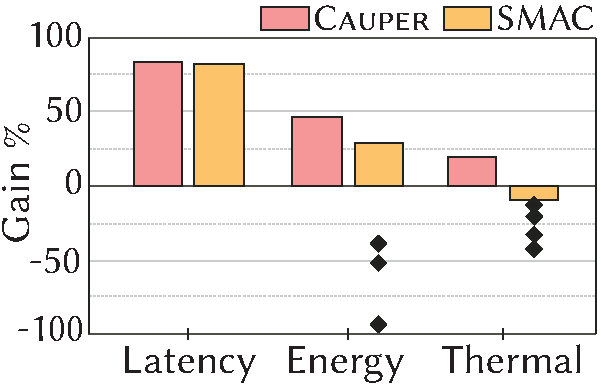
\includegraphics[width=0.3\linewidth]{fig__rq3_a.pdf}
    %     \label{fig:rq3_1_a}
    % }\quad
    \subfloat[Latency]{ \vspace{-1.5em}
        \includegraphics[width=\linewidth]{figures-vg/latency_eff.pdf}
        \label{fig:rq2_1}
    }\\
    \vspace{-1.5em}
    \subfloat[Energy]{
        \includegraphics[width=\linewidth]{figures-vg/energy_eff.pdf}
        \label{fig:rq2_2}
    }
    % \subfloat[Multi Objective]{
    %     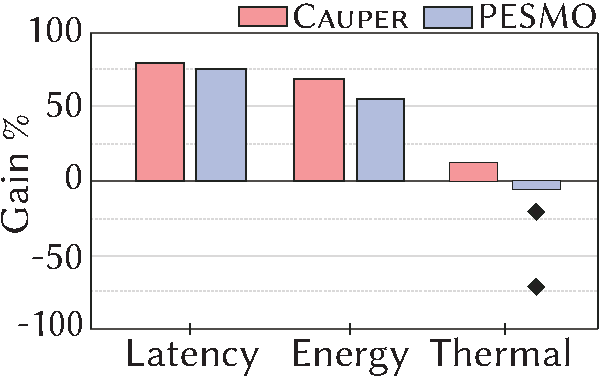
\includegraphics[width=0.275\linewidth]{fig__rq3_b.pdf}
    %     \label{fig:rq3_1_b}
    % }
 
    \caption{\small{\ourapproach has significantly higher sampling efficiency than other baselines in debugging non-functional faults: (a) latency faults in \txtwo and (b) energy faults in \xavier.}}% (indicated by $\blacklozenge$).}}
    \label{tab:rq2_1}
\end{figure}
\noindent{\textbf{Results (debugging).}}~\Cref{tab:single_1,tab:multi_1} shows \ourapproach ~{\em significantly outperforms correlation-based methods in all cases}. For example, in  \textsc{Deepstream} on TX2, \ourapproach achieves 6\% more accuracy, 12\% more precision, and 10\% more recall compared to the next best method, \bugdoc. We observed latency gains as high as $88\%$ ($9\%$ more than \bugdoc) on \txtwo and energy gain of $86\%$ ($9\%$ more than \bugdoc) on \xavier for \textsc{Xception}. We observe similar trends for multi-objective faults as well. The results confirm that \ourapproach~{\em can recommend repairs for faults that significantly improve latency and energy}. By applying the changes to the configurations recommended by \ourapproach improves performance drastically. 


\fig{rq2_1} and \fig{rq2_2} demonstrate the sample efficiency results for different systems. We observe that, for both latency and energy faults, \ourapproach achieved significantly higher gains with substantially fewer samples. For \textsc{Xception}, \ourapproach required a 8$\times$ fewer samples to obtain 32\% higher gain than \textsc{DD}. The higher gain in \ourapproach in comparison to correlation-based methods indicates that \ourapproach's causal reasoning is more effective in guiding the search in the objective space. \ourapproach does not waste budget evaluating configurations with lower causal effects and finds a fix faster.

\begin{figure}[tp!]
    % \subfloat[\tool vs. SMAC for resolving \\latency faults.]{
    %     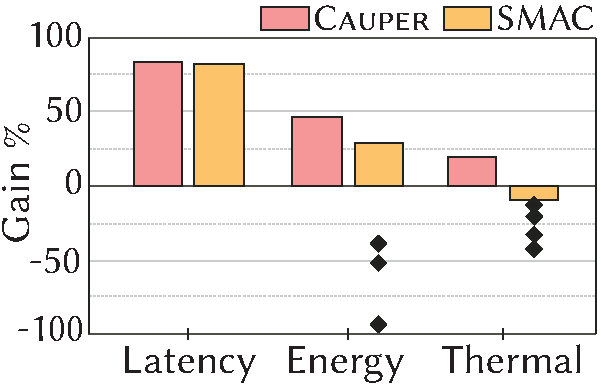
\includegraphics[width=0.3\linewidth]{fig__rq3_a.pdf}
    %     \label{fig:rq3_1_a}
    % }\quad
  
    \includegraphics[width=\linewidth]{figures-vg/sobo_opt_tx2.pdf} 
    \includegraphics[width=\linewidth]{figures-vg/mobo_opt_tx2.pdf}
    \vspace{-4mm}
    \caption{\small{\ourapproach vs. single and multi-objective optimization with SMAC and PESMO in \txtwo.}}% (indicated by $\blacklozenge$).}}
     \label{fig:rq1_opt_se}
    \vspace{-3mm}
\end{figure}

\ourapproach~{\em resolves misconfiguration faults significantly faster than correlation-based approaches}. In~\Cref{tab:single_1,tab:multi_1}, the last two columns indicate the time taken (in hours) by each approach to diagnosing the root cause. For all correlation-based methods, we set a maximum budget of 4 hours. We find that, while other approaches use the entire budget to diagnose and resolve the faults, \ourapproach can do so significantly faster. In particular, we observed that \ourapproach is $13\times$ faster in diagnosing and resolving faults in energy usage for \textsc{x264} deployed on \xavier and $10\times$ faster for latency faults for \textsc{Bert} deployed on \txtwo. 

% All the methods found it difficult to discover the root cause of thermal faults. While \tool outperforms other methods, the overall accuracy, precision, recall, and $\Delta_{gain}$ were lower than corresponding values for latency and energy consumption faults. This is because we performed thermal measurements in a controlled environment to prevent thermal throttling the variance in the measurements was relatively lower than latency and energy consumption.



% \noindent \textbf{Task2. Optimization}
% Here, we employ the learned SCM~\rayb{What is SCM?} as the surrogate model and causal reasoning of effect estimation as the acquisition function for effective exploration of the search space. Mechanisms of counterfactual query evaluation and intervention provide the necessary exploration-exploitation tradeoff.
% The first two phases of \tool is the same as the debugging non-functional fault task. In Phase-III, we use the following queries for single-objective optimization of latency or energy: "\textit{How to improve latency/energy from the optimal so far?}". \tool can natively accommodate multi-objective optimization by slightly altering the counterfactual query. For multi-objective latency and/or energy fault we use the following query: "\textit{How to improve latency or energy by from the optimal observed so far?}". We continue incremental learning until no new configurations are found or the maximum budget of 4 hours is exhausted, whichever occurs first, and return the configuration with minimum latency or energy obtained thus far.

% \noindent \textbf{Setting.}
% For single-objective optimization, we compare \tool with SMAC in \txtwo for \textsc{Xception} for both latency and energy. For multi-objective optimization, PESMO~\cite{hernandez2016predictive} to find a configuration that optimizes for energy and latency simultaneously. We repeat the entire process 3 times for consistent analyses.

% Out of 21 latency faults in image recognition on \txtwo, we found 7 cases (33\%) where the near-optimal configuration caused a significant deterioration in energy consumption. In one case the optimal configuration increased the energy consumption by $96\%$! 
% \noindent\textit{$\circ$~Why \tool works better?}~
% \tool never deteriorates any non-functional property. This is a desirable benefit of using causal graphs. For example, if \tool notices that a configuration option (say) \texttt{GPU frequency} affects both latency and energy consumption, \tool would not recommend changing \texttt{GPU  frequency} to the extent where it consumes too much energy. By design, \tool would explore the possibility of changing other configuration options to improve latency. Optimization approaches are not equipped to handle this. 
 %Note that, while PESMO did not find a configuration that caused high energy consumption, it still suffered from deterioration in heat dissipation in two cases. 


\noindent\textbf{Results (optimization).}~\fig{rq1_opt_se}(a) and \fig{rq1_opt_se}(b) demonstrate the single-objective optimization results---\ourapproach finds configurations with optimal latency and energy for both cases. \fig{rq1_opt_se}(a)  illustrates that the optimal configuration discovered by \ourapproach has 43\% lower latency (12 seconds) than that of SMAC (21 seconds). Here, \ourapproach reaches near-optimal configuration by only exhausting one-third of the entire budget. In \fig{rq1_opt_se}(b), the optimal configuration discovered by \ourapproach and SMAC had almost the same energy, but \ourapproach reached this optimal configuration 4x faster than SMAC. In both single-objective optimizations, the iterative variation of \ourapproach is less than SMAC--i.e., \ourapproach finds more stable configurations. \fig{rq1_opt_se}(c) compares \ourapproach with PESMO to optimize both latency and energy in \txtwo (for image recognition). Here, \ourapproach has 12\% lower hypervolume error than  PESMO and reaches the same level of hypervolume error of PESMO 4x times faster. \fig{rq1_opt_se}(d) illustrates the Pareto optimal configurations obtained by \ourapproach and PESMO. The Pareto front discovered by \ourapproach has higher coverage, as it discovers a larger number of Pareto optimal configurations with lower energy and latency value than PESMO.

% \noindent{\textbf{Discussion.}}~Correlation-based methods rely only on correlation, and this can be misleading since they cannot incorporate the intrinsic complex causal structure of the underlying configuration space. In contrast, \tool relies on causal inference (instead of correlation) to model the configuration space thereby overcoming the limitations with current correlation-based models. Correlation-based methods require a large number of initial observational data for training. They spend most of their allocated 4-hour budget on gathering these training samples. In contrast, \tool starts with only 25 samples and uses incremental learning (\tion{incremental_learning}) to judiciously update the casual graph with better samples that capture the relationships in the search space better. 

%ML-based methods require a large number of initial observational data for training. They expend most of their allocated 4-hour budget on gathering these training samples. In contrast, \tool starts with only 25 samples and uses incremental learning (\tion{incremental_learning}) to judiciously update the casual graph with new configurations until a repair has been found. This drastically reduces the inference time.% and also improves diagnostic capability. %Further, the incremental learning  

% {\em Default configurations perform poorly:} An alternate approach to finding root-cause of a non-functional fault is to compare which configurations in non-functional fault differed from the default configuration. Doing so results in poor performance. The accuracy, precision, and recall were often less than 50\%.


% {\em The cases where CBI is better than} \tool:~
% In one case, with BERT (NLP), deployed on TX2, CBI performs slightly better than \tool, \ie, CBI achieves an accuracy of 68\% and recall of 69\% whereas \tool achieves an accuracy of 64\% and recall of 62\%. However, this comes at a cost of lower precision (57\% in CBI vs. 77\% in \tool); this indicates that CBI detects a large number of false positives. False positives can be detrimental to improving performance. Specifically, for the same case of BERT$\longrightarrow$TX2 in~\tab{rq1_2}, we see that \tool recommends more useful repairs than CBI, \ie, \tool gives us a performance gain of $96\%$ compared to only $76\%$ from CBI.
% \ei
% \noindent\textbf{Why \tool works better?}
% % In general, our results highlight the usefulness of causal models and counterfactual inference that differentiate them from ML-based approaches. 
% \tool uses a causal model to express the complex relationships between configurations and performance and uses this to diagnose the root cause of non-functional faults. Further, using counterfactual inference over the causal model, \tool can recommend useful fixes using only the current observational data. ML-based approaches are limited in this respect. They fail to model the complex interactions between various configuration options and they can only use the observational data provided to them to draw their inferences. They require additional data to build reliable models. This can be both expensive and time-consuming. %In contrast, \tool uses incremental learning 

% \noindent{\textbf{RQ1-B. How effective is \tool in diagnosing multi-objective faults?}}
% 
% %  \begin{table}[]
%      \centering
%      \caption{\small (RQ2) Efficiency of \tool in detecting and repairing the root-cause of multiple non-functional faults. Cells highlighted in \colorbox{blue!10}{green} indicate better performance and \colorbox[HTML]{FFCCC9}{red} indicate cases where the performance drops. Note: the results are reported for two kinds of faults in TX2: (1) faults in both latency and energy; and (2) faults in latency, energy, and heat dissipation.}
%      \label{tab:rq2}
%      \resizebox{\linewidth}{!}{
%      \begin{tabular}{ll|rr|rr|rr|}
%       &  & \multicolumn{1}{r|}{\rotatebox{90}{\tool}} & \rotatebox{90}{Default} & \multicolumn{1}{r|}{\rotatebox{90}{\tool}} & \rotatebox{90}{Default} & \multicolumn{1}{r|}{\rotatebox{90}{\tool}} & \multicolumn{1}{r|}{\rotatebox{90}{Default}} \bigstrut\\ \cline{3-8} 
%       & Software & \multicolumn{2}{r|}{Accuracy} & \multicolumn{2}{r|}{Recall} & \multicolumn{2}{r|}{Precision} \bigstrut\\ \hlineB{2}
%      \multicolumn{1}{l|}{\multirow{6.5}{*}{Latency and Energy}} & DNN Image & \cellcolor{blue!10}59 & 51 & \cellcolor{blue!10}44 & 35 & \cellcolor{blue!10}65 & 56 \bigstrut\\
%      \multicolumn{1}{l|}{} & DNN   Speech & \cellcolor{blue!10}66 & 49 & \cellcolor{blue!10}51 & 43 & \cellcolor{blue!10}74 & 64 \bigstrut\\
%      \multicolumn{1}{l|}{} & DNN NLP & \cellcolor{blue!10}56 & 53 & \cellcolor{blue!10}42 & \cellcolor{blue!10}42 & \cellcolor{blue!10}66 & 61 \bigstrut\\
%      \multicolumn{1}{l|}{} & x264 & \cellcolor{blue!10}51 & 48 & \cellcolor{blue!10}55 & 33 & \cellcolor{blue!10}64 & 56 \bigstrut\\
%      \multicolumn{1}{l|}{} & SQLite & \cellcolor{blue!10}60 & 51 & \cellcolor{blue!10}57 & 37 & \cellcolor{blue!10}72 & 57 \bigstrut\\ \hlineB{2}
%      \multicolumn{1}{l|}{\multirow{3}{*}{All three}} & DNN Image & \cellcolor{blue!10}67 & 59 & \cellcolor{blue!10}69 & 60 & \cellcolor{blue!10}64 & 60 \bigstrut\\
%      \multicolumn{1}{l|}{} & x264 & \cellcolor{blue!10}68 & 62 & \cellcolor{blue!10}79 & 56 & \cellcolor{blue!10}68 & 58 \bigstrut\\
%      \multicolumn{1}{l|}{} & SQLite & \cellcolor{blue!10}79 & 63 & \cellcolor{blue!10}70 & 57 & \cellcolor{blue!10}84 & 63 \bigstrut\\ \hlineB{2}\multicolumn{1}{l}{}&\multicolumn{1}{l}{}&\multicolumn{1}{l}{}&\multicolumn{1}{l}{}&\multicolumn{1}{l}{}&\multicolumn{1}{l}{}&\multicolumn{1}{l}{}\bigstrut\\[-0.4cm]\hlineB{2}
%      \multicolumn{1}{l}{\multirow{9.5}{*}{Latency and Energy}} & \multicolumn{1}{r|}{$\Delta_{gain}\longrightarrow$} & \multicolumn{2}{c|}{{Latency}} & \multicolumn{2}{c|}{{Energy}} & \multicolumn{2}{c|}{{Thermals}} \bigstrut\\ \hlineB{2} 
    
%      \multicolumn{1}{l|}{} & DNN Image & \cellcolor{blue!10}52 & \multicolumn{1}{l|}{33} & \multicolumn{1}{l}{\cellcolor{blue!10}37} & \multicolumn{1}{l|}{22} & \multicolumn{1}{l}{0} & \multicolumn{1}{l|}{0} \bigstrut\\
    
%      \multicolumn{1}{l|}{} & DNN   Speech & \multicolumn{1}{l}{\cellcolor{blue!10}60} & \multicolumn{1}{l|}{25} & \multicolumn{1}{l}{\cellcolor{blue!10}54} & \multicolumn{1}{l|}{17} & \multicolumn{1}{l}{0} & \multicolumn{1}{l|}{0} \bigstrut\\
    
%      \multicolumn{1}{l|}{} & DNN NLP & \multicolumn{1}{l}{\cellcolor{blue!10}49} & \multicolumn{1}{l|}{30} & \multicolumn{1}{l}{\cellcolor{blue!10}51} & \multicolumn{1}{l|}{17} & \multicolumn{1}{l}{0} & \multicolumn{1}{l|}{0} \bigstrut\\
    
%      \multicolumn{1}{l|}{} & x264 & \multicolumn{1}{l}{\cellcolor{blue!10}23} & \multicolumn{1}{l|}{2} & \multicolumn{1}{l}{\cellcolor{blue!10}12} & \multicolumn{1}{l|}{\cellcolor[HTML]{FFCCC9}-2} & \multicolumn{1}{l}{0} & \multicolumn{1}{l|}{\cellcolor[HTML]{FFCCC9}-1} \bigstrut\\
    
%      \multicolumn{1}{l|}{} & SQLite & \multicolumn{1}{l}{\cellcolor{blue!10}9} & \multicolumn{1}{l|}{6} & \multicolumn{1}{l}{\cellcolor{blue!10}11} & \multicolumn{1}{l|}{2} & \multicolumn{1}{l}{0} & \multicolumn{1}{l|}{\cellcolor[HTML]{FFCCC9}-1} \bigstrut\\ \hlineB{2}
    
%      \multicolumn{1}{l|}{\multirow{3}{*}{All three}} & DNN Image & \multicolumn{1}{l}{\cellcolor{blue!10}54} & \multicolumn{1}{l|}{29} & \multicolumn{1}{l}{\cellcolor{blue!10}31} & \multicolumn{1}{l|}{16} & \multicolumn{1}{l}{1} & \multicolumn{1}{l|}{1} \bigstrut\\
    
%      \multicolumn{1}{l|}{} & x264 & \multicolumn{1}{l}{\cellcolor{blue!10}18} & \multicolumn{1}{l|}{1} & \multicolumn{1}{l}{\cellcolor{blue!10}10} & \multicolumn{1}{l|}{\cellcolor[HTML]{FFCCC9}-1} & \multicolumn{1}{l}{1} & \multicolumn{1}{l|}{\cellcolor[HTML]{FFCCC9}-1} \bigstrut\\
   
%      \multicolumn{1}{l|}{} & SQLite & \multicolumn{1}{l}{\cellcolor{blue!10}6} & \multicolumn{1}{l|}{3} & \multicolumn{1}{l}{\cellcolor{blue!10}7} & \multicolumn{1}{l|}{2} & \multicolumn{1}{l}{1} & \multicolumn{1}{l|}{0} \bigstrut\\ \hlineB{2}
%      \end{tabular}
%      }
%      \end{table}

\begin{table*}[]
    \centering
    \caption{\small {Efficiency of \tool in detecting and repairing the root-cause of multiple non-functional faults: \textit{Energy, Latency}; and \textit{Energy, Latency, Heat}. Cells highlighted in \colorbox{blue!10}{green} indicate improvement over faults and \colorbox[HTML]{FFCCC9}{red} indicate deterioration. \tool achieves better performance overall and is much faster. Note: the results are reported for NVIDIA Jetson TX2.}}
    \label{tab:rq2}
    \footnotesize
    \resizebox{\textwidth}{!}{
        \begin{tabular}{@{}l@{}ll|llll|llll|llll|llll|llll|llll|ll|}
            \clineB{4-29}{2}
            &  &  & \multicolumn{4}{c|}{Accuracy} & \multicolumn{4}{c|}{Precision} & \multicolumn{4}{c|}{Recall} & \multicolumn{4}{c|}{Gain (Latency)} & \multicolumn{4}{c|}{Gain (Energy)} & \multicolumn{4}{c|}{Gain (Heat)} & \multicolumn{2}{c|}{Time$^\dagger$} \bigstrut\\ \clineB{4-29}{2}
            % &  &  &  &  &  &  &  &  & \\[-1em]\clineB{4-29}{2} 
            
            &  &  & \rotatebox{90}{\bfseries\tool~} & \rotatebox{90}{\cbi} & \rotatebox{90}{\encore} & \rotatebox{90}{\bugdoc} & \rotatebox{90}{\bfseries\tool~} & \rotatebox{90}{\cbi} & \rotatebox{90}{\encore} & \rotatebox{90}{\bugdoc} & \rotatebox{90}{\bfseries\tool~} & \rotatebox{90}{\cbi} & \rotatebox{90}{\encore} & \rotatebox{90}{\bugdoc} & \rotatebox{90}{\bfseries\tool~} & \rotatebox{90}{\cbi} & \rotatebox{90}{\encore} & \rotatebox{90}{\bugdoc} & \rotatebox{90}{\bfseries\tool~} & \rotatebox{90}{\cbi} & \rotatebox{90}{\encore} & \rotatebox{90}{\bugdoc} & \rotatebox{90}{\bfseries\tool~} & \rotatebox{90}{\cbi} & \rotatebox{90}{\encore} & \rotatebox{90}{\bugdoc} & \rotatebox{90}{\bfseries\tool~} & \rotatebox{90}{Others} \\ \clineB{4-29}{2}
            
            \multicolumn{1}{l}{}&\multicolumn{1}{l}{}  & \multicolumn{1}{l}{} & \multicolumn{1}{l}{} & \multicolumn{1}{l}{} & \multicolumn{1}{l}{} & \multicolumn{1}{l}{} & \multicolumn{1}{l}{} & \multicolumn{1}{l}{} & \multicolumn{1}{l}{} \\[-0.9em]\hlineB{2}

            & \multicolumn{1}{l|}{} & Image & \cellcolor{blue!10}\textbf{77} & 54 & 55 & 65 & \cellcolor{blue!10}\textbf{73} & 53 & 54 & 62 & \cellcolor{blue!10}\textbf{80} & 59 & 59 & 62 & \cellcolor{blue!10}\textbf{83} & 53 & 61 & 65 & \cellcolor{blue!10}\textbf{70} & 38 & 46 & 44 & \cellcolor{blue!10}\textbf{3} & 0 & 0 & 0 & \cellcolor{blue!10}\textbf{0.6} & 4 \\
            & \multicolumn{1}{l|}{} & NLP & \cellcolor{blue!10}\textbf{70} & 51 & 56 & 65 & \cellcolor{blue!10}\textbf{71} & 42 & 56 & 63 & \cellcolor{blue!10}\textbf{66} & 59 & 62 & 65 & \cellcolor{blue!10}\textbf{68} & 53 & 59 & 61 & \cellcolor{blue!10}\textbf{60} & 41 & 27 & 48 & \cellcolor{blue!10}\textbf{5} & 0 & 0 & 1 & \cellcolor{blue!10}\textbf{0.2} & 4 \\
            & \multicolumn{1}{l|}{} & Speech & \cellcolor{blue!10}\textbf{74} & 50 & 61 & 65 & \cellcolor{blue!10}\textbf{68} & 44 & 53 & 62 & \cellcolor{blue!10}\textbf{79} & 51 & 59 & 64 & \cellcolor{blue!10}\textbf{82} & 55 & 55 & 62 & \cellcolor{blue!10}\textbf{66} & 43 & 43 & 41 & \cellcolor{blue!10}\textbf{4} & \cellcolor[HTML]{FFCCC9}-2 & \cellcolor[HTML]{FFCCC9}-1 & \cellcolor[HTML]{FFCCC9}-1 & \cellcolor{blue!10}\textbf{0.7} & 4 \\
            & \multicolumn{1}{l|}{} & x264 & \cellcolor{blue!10}\textbf{83} & 54 & 55 & 66 & \cellcolor{blue!10}\textbf{81} & 50 & 54 & 57 & \cellcolor{blue!10}\textbf{77} & 63 & 62 & 61 & \cellcolor{blue!10}\textbf{15} & 2 & 4 & 6 & \cellcolor{blue!10}\textbf{13} & 4 & 6 & 4 & \cellcolor{blue!10}\textbf{2} & \cellcolor[HTML]{FFCCC9}-3 & \cellcolor[HTML]{FFCCC9}-1 & 0 & \cellcolor{blue!10}\textbf{1.2} & 4 \\
           \multirow{-5}{*}{\rotatebox{90}{Energy +}} & \multicolumn{1}{l|}{\multirow{-5}{*}{\rotatebox{90}{Latency}}} & SQLite & \cellcolor{blue!10}\textbf{84} & 51 & 58 & 68 & \cellcolor{blue!10}\textbf{80} & 43 & 55 & 62 & \cellcolor{blue!10}\textbf{84} & 57 & 63 & 65 & \cellcolor{blue!10}\textbf{11} & 5 & 4 & 5 & \cellcolor{blue!10}\textbf{14} & 3 & 8 & 8 & \cellcolor{blue!10}\textbf{2} & \cellcolor[HTML]{FFCCC9}-2 & 0 & \cellcolor[HTML]{FFCCC9}-1 & \cellcolor{blue!10}\textbf{0.5} & 4 \\ \hlineB{2}

           \multicolumn{1}{l}{}&\multicolumn{1}{l}{}  & \multicolumn{1}{l}{} & \multicolumn{1}{l}{} & \multicolumn{1}{l}{} & \multicolumn{1}{l}{} & \multicolumn{1}{l}{} & \multicolumn{1}{l}{} & \multicolumn{1}{l}{} & \multicolumn{1}{l}{} \\[-0.95em]\hlineB{2}

            & \multicolumn{1}{l|}{} & Image & \cellcolor{blue!10}\textbf{76} & 57 & 48 & 66 & \cellcolor{blue!10}\textbf{68} & 61 & 57 & 61 & \cellcolor{blue!10}\textbf{81} & 53 & 46 & 70 & \cellcolor{blue!10}\textbf{62} & 33 & 30 & 42 & \cellcolor{blue!10}\textbf{52} & 23 & 18 & 24 & \cellcolor{blue!10}\textbf{4} & 1 & 0 & 0 & \cellcolor{blue!10}\textbf{0.1} & 4 \\
            & \multicolumn{1}{l|}{} & x264 & \cellcolor{blue!10}\textbf{80} & 59 & 47 & 54 & \cellcolor{blue!10}\textbf{76} & 61 & 56 & 63 & \cellcolor{blue!10}\textbf{81} & 56 & 46 & 51 & \cellcolor{blue!10}\textbf{12} & 2 & 1 & 2 & \cellcolor{blue!10}\textbf{15} & 4 & 2 & 4 & \cellcolor{blue!10}\textbf{4} & 1 & 0 & 1 & \cellcolor{blue!10}\textbf{0.1} & 4 \\
           \multirow{-3}{*}{\rotatebox{90}{All}} & \multicolumn{1}{l|}{\multirow{-3}{*}{\rotatebox{90}{Three}}} & SQLite & \cellcolor{blue!10}\textbf{73} & 56 & 51 & 53 & \cellcolor{blue!10}\textbf{68} & 59 & 56 & 60 & \cellcolor{blue!10}\textbf{78} & 54 & 45 & 51 & \cellcolor{blue!10}\textbf{12} & 1 & 1 & 4 & \cellcolor{blue!10}\textbf{8} & 4 & 2 & 5 & \cellcolor{blue!10}\textbf{1} & 1 & \cellcolor[HTML]{FFCCC9}-1 & \cellcolor[HTML]{FFCCC9}-1 & \cellcolor{blue!10}\textbf{0.1} & 4 \\ \hlineB{2}
           \multicolumn{10}{l}{$^\dagger$ Wallclock time in hours}\bigstrut
           \end{tabular}
    }
\end{table*}
    
% This RQ focuses on multi-objective faults where misconfigurations affect multiple non-functional properties simultaneously, \ie, in latency \textit{and} energy consumption. %In this section, 
% we emulate the scenario where a user experiences such multi-objective faults and uses \tool to help answer the following two questions:
% \bi[leftmargin=*]
% \item What is the root cause of my non-functional fault? 
% \item What can I change to repair my performance on the faulty objectives while not degrading the correctly functioning objectives?
% \ei
% Similar to RQ1, 
% we evaluate how well \tool can diagnose and fix such faults.
% 
% %  \begin{table}[]
%      \centering
%      \caption{\small (RQ2) Efficiency of \tool in detecting and repairing the root-cause of multiple non-functional faults. Cells highlighted in \colorbox{blue!10}{green} indicate better performance and \colorbox[HTML]{FFCCC9}{red} indicate cases where the performance drops. Note: the results are reported for two kinds of faults in TX2: (1) faults in both latency and energy; and (2) faults in latency, energy, and heat dissipation.}
%      \label{tab:rq2}
%      \resizebox{\linewidth}{!}{
%      \begin{tabular}{ll|rr|rr|rr|}
%       &  & \multicolumn{1}{r|}{\rotatebox{90}{\tool}} & \rotatebox{90}{Default} & \multicolumn{1}{r|}{\rotatebox{90}{\tool}} & \rotatebox{90}{Default} & \multicolumn{1}{r|}{\rotatebox{90}{\tool}} & \multicolumn{1}{r|}{\rotatebox{90}{Default}} \bigstrut\\ \cline{3-8} 
%       & Software & \multicolumn{2}{r|}{Accuracy} & \multicolumn{2}{r|}{Recall} & \multicolumn{2}{r|}{Precision} \bigstrut\\ \hlineB{2}
%      \multicolumn{1}{l|}{\multirow{6.5}{*}{Latency and Energy}} & DNN Image & \cellcolor{blue!10}59 & 51 & \cellcolor{blue!10}44 & 35 & \cellcolor{blue!10}65 & 56 \bigstrut\\
%      \multicolumn{1}{l|}{} & DNN   Speech & \cellcolor{blue!10}66 & 49 & \cellcolor{blue!10}51 & 43 & \cellcolor{blue!10}74 & 64 \bigstrut\\
%      \multicolumn{1}{l|}{} & DNN NLP & \cellcolor{blue!10}56 & 53 & \cellcolor{blue!10}42 & \cellcolor{blue!10}42 & \cellcolor{blue!10}66 & 61 \bigstrut\\
%      \multicolumn{1}{l|}{} & x264 & \cellcolor{blue!10}51 & 48 & \cellcolor{blue!10}55 & 33 & \cellcolor{blue!10}64 & 56 \bigstrut\\
%      \multicolumn{1}{l|}{} & SQLite & \cellcolor{blue!10}60 & 51 & \cellcolor{blue!10}57 & 37 & \cellcolor{blue!10}72 & 57 \bigstrut\\ \hlineB{2}
%      \multicolumn{1}{l|}{\multirow{3}{*}{All three}} & DNN Image & \cellcolor{blue!10}67 & 59 & \cellcolor{blue!10}69 & 60 & \cellcolor{blue!10}64 & 60 \bigstrut\\
%      \multicolumn{1}{l|}{} & x264 & \cellcolor{blue!10}68 & 62 & \cellcolor{blue!10}79 & 56 & \cellcolor{blue!10}68 & 58 \bigstrut\\
%      \multicolumn{1}{l|}{} & SQLite & \cellcolor{blue!10}79 & 63 & \cellcolor{blue!10}70 & 57 & \cellcolor{blue!10}84 & 63 \bigstrut\\ \hlineB{2}\multicolumn{1}{l}{}&\multicolumn{1}{l}{}&\multicolumn{1}{l}{}&\multicolumn{1}{l}{}&\multicolumn{1}{l}{}&\multicolumn{1}{l}{}&\multicolumn{1}{l}{}\bigstrut\\[-0.4cm]\hlineB{2}
%      \multicolumn{1}{l}{\multirow{9.5}{*}{Latency and Energy}} & \multicolumn{1}{r|}{$\Delta_{gain}\longrightarrow$} & \multicolumn{2}{c|}{{Latency}} & \multicolumn{2}{c|}{{Energy}} & \multicolumn{2}{c|}{{Thermals}} \bigstrut\\ \hlineB{2} 
    
%      \multicolumn{1}{l|}{} & DNN Image & \cellcolor{blue!10}52 & \multicolumn{1}{l|}{33} & \multicolumn{1}{l}{\cellcolor{blue!10}37} & \multicolumn{1}{l|}{22} & \multicolumn{1}{l}{0} & \multicolumn{1}{l|}{0} \bigstrut\\
    
%      \multicolumn{1}{l|}{} & DNN   Speech & \multicolumn{1}{l}{\cellcolor{blue!10}60} & \multicolumn{1}{l|}{25} & \multicolumn{1}{l}{\cellcolor{blue!10}54} & \multicolumn{1}{l|}{17} & \multicolumn{1}{l}{0} & \multicolumn{1}{l|}{0} \bigstrut\\
    
%      \multicolumn{1}{l|}{} & DNN NLP & \multicolumn{1}{l}{\cellcolor{blue!10}49} & \multicolumn{1}{l|}{30} & \multicolumn{1}{l}{\cellcolor{blue!10}51} & \multicolumn{1}{l|}{17} & \multicolumn{1}{l}{0} & \multicolumn{1}{l|}{0} \bigstrut\\
    
%      \multicolumn{1}{l|}{} & x264 & \multicolumn{1}{l}{\cellcolor{blue!10}23} & \multicolumn{1}{l|}{2} & \multicolumn{1}{l}{\cellcolor{blue!10}12} & \multicolumn{1}{l|}{\cellcolor[HTML]{FFCCC9}-2} & \multicolumn{1}{l}{0} & \multicolumn{1}{l|}{\cellcolor[HTML]{FFCCC9}-1} \bigstrut\\
    
%      \multicolumn{1}{l|}{} & SQLite & \multicolumn{1}{l}{\cellcolor{blue!10}9} & \multicolumn{1}{l|}{6} & \multicolumn{1}{l}{\cellcolor{blue!10}11} & \multicolumn{1}{l|}{2} & \multicolumn{1}{l}{0} & \multicolumn{1}{l|}{\cellcolor[HTML]{FFCCC9}-1} \bigstrut\\ \hlineB{2}
    
%      \multicolumn{1}{l|}{\multirow{3}{*}{All three}} & DNN Image & \multicolumn{1}{l}{\cellcolor{blue!10}54} & \multicolumn{1}{l|}{29} & \multicolumn{1}{l}{\cellcolor{blue!10}31} & \multicolumn{1}{l|}{16} & \multicolumn{1}{l}{1} & \multicolumn{1}{l|}{1} \bigstrut\\
    
%      \multicolumn{1}{l|}{} & x264 & \multicolumn{1}{l}{\cellcolor{blue!10}18} & \multicolumn{1}{l|}{1} & \multicolumn{1}{l}{\cellcolor{blue!10}10} & \multicolumn{1}{l|}{\cellcolor[HTML]{FFCCC9}-1} & \multicolumn{1}{l}{1} & \multicolumn{1}{l|}{\cellcolor[HTML]{FFCCC9}-1} \bigstrut\\
   
%      \multicolumn{1}{l|}{} & SQLite & \multicolumn{1}{l}{\cellcolor{blue!10}6} & \multicolumn{1}{l|}{3} & \multicolumn{1}{l}{\cellcolor{blue!10}7} & \multicolumn{1}{l|}{2} & \multicolumn{1}{l}{1} & \multicolumn{1}{l|}{0} \bigstrut\\ \hlineB{2}
%      \end{tabular}
%      }
%      \end{table}

\begin{table*}[]
    \centering
    \caption{\small {Efficiency of \tool in detecting and repairing the root-cause of multiple non-functional faults: \textit{Energy, Latency}; and \textit{Energy, Latency, Heat}. Cells highlighted in \colorbox{blue!10}{green} indicate improvement over faults and \colorbox[HTML]{FFCCC9}{red} indicate deterioration. \tool achieves better performance overall and is much faster. Note: the results are reported for NVIDIA Jetson TX2.}}
    \label{tab:rq2}
    \footnotesize
    \resizebox{\textwidth}{!}{
        \begin{tabular}{@{}l@{}ll|llll|llll|llll|llll|llll|llll|ll|}
            \clineB{4-29}{2}
            &  &  & \multicolumn{4}{c|}{Accuracy} & \multicolumn{4}{c|}{Precision} & \multicolumn{4}{c|}{Recall} & \multicolumn{4}{c|}{Gain (Latency)} & \multicolumn{4}{c|}{Gain (Energy)} & \multicolumn{4}{c|}{Gain (Heat)} & \multicolumn{2}{c|}{Time$^\dagger$} \bigstrut\\ \clineB{4-29}{2}
            % &  &  &  &  &  &  &  &  & \\[-1em]\clineB{4-29}{2} 
            
            &  &  & \rotatebox{90}{\bfseries\tool~} & \rotatebox{90}{\cbi} & \rotatebox{90}{\encore} & \rotatebox{90}{\bugdoc} & \rotatebox{90}{\bfseries\tool~} & \rotatebox{90}{\cbi} & \rotatebox{90}{\encore} & \rotatebox{90}{\bugdoc} & \rotatebox{90}{\bfseries\tool~} & \rotatebox{90}{\cbi} & \rotatebox{90}{\encore} & \rotatebox{90}{\bugdoc} & \rotatebox{90}{\bfseries\tool~} & \rotatebox{90}{\cbi} & \rotatebox{90}{\encore} & \rotatebox{90}{\bugdoc} & \rotatebox{90}{\bfseries\tool~} & \rotatebox{90}{\cbi} & \rotatebox{90}{\encore} & \rotatebox{90}{\bugdoc} & \rotatebox{90}{\bfseries\tool~} & \rotatebox{90}{\cbi} & \rotatebox{90}{\encore} & \rotatebox{90}{\bugdoc} & \rotatebox{90}{\bfseries\tool~} & \rotatebox{90}{Others} \\ \clineB{4-29}{2}
            
            \multicolumn{1}{l}{}&\multicolumn{1}{l}{}  & \multicolumn{1}{l}{} & \multicolumn{1}{l}{} & \multicolumn{1}{l}{} & \multicolumn{1}{l}{} & \multicolumn{1}{l}{} & \multicolumn{1}{l}{} & \multicolumn{1}{l}{} & \multicolumn{1}{l}{} \\[-0.9em]\hlineB{2}

            & \multicolumn{1}{l|}{} & Image & \cellcolor{blue!10}\textbf{77} & 54 & 55 & 65 & \cellcolor{blue!10}\textbf{73} & 53 & 54 & 62 & \cellcolor{blue!10}\textbf{80} & 59 & 59 & 62 & \cellcolor{blue!10}\textbf{83} & 53 & 61 & 65 & \cellcolor{blue!10}\textbf{70} & 38 & 46 & 44 & \cellcolor{blue!10}\textbf{3} & 0 & 0 & 0 & \cellcolor{blue!10}\textbf{0.6} & 4 \\
            & \multicolumn{1}{l|}{} & NLP & \cellcolor{blue!10}\textbf{70} & 51 & 56 & 65 & \cellcolor{blue!10}\textbf{71} & 42 & 56 & 63 & \cellcolor{blue!10}\textbf{66} & 59 & 62 & 65 & \cellcolor{blue!10}\textbf{68} & 53 & 59 & 61 & \cellcolor{blue!10}\textbf{60} & 41 & 27 & 48 & \cellcolor{blue!10}\textbf{5} & 0 & 0 & 1 & \cellcolor{blue!10}\textbf{0.2} & 4 \\
            & \multicolumn{1}{l|}{} & Speech & \cellcolor{blue!10}\textbf{74} & 50 & 61 & 65 & \cellcolor{blue!10}\textbf{68} & 44 & 53 & 62 & \cellcolor{blue!10}\textbf{79} & 51 & 59 & 64 & \cellcolor{blue!10}\textbf{82} & 55 & 55 & 62 & \cellcolor{blue!10}\textbf{66} & 43 & 43 & 41 & \cellcolor{blue!10}\textbf{4} & \cellcolor[HTML]{FFCCC9}-2 & \cellcolor[HTML]{FFCCC9}-1 & \cellcolor[HTML]{FFCCC9}-1 & \cellcolor{blue!10}\textbf{0.7} & 4 \\
            & \multicolumn{1}{l|}{} & x264 & \cellcolor{blue!10}\textbf{83} & 54 & 55 & 66 & \cellcolor{blue!10}\textbf{81} & 50 & 54 & 57 & \cellcolor{blue!10}\textbf{77} & 63 & 62 & 61 & \cellcolor{blue!10}\textbf{15} & 2 & 4 & 6 & \cellcolor{blue!10}\textbf{13} & 4 & 6 & 4 & \cellcolor{blue!10}\textbf{2} & \cellcolor[HTML]{FFCCC9}-3 & \cellcolor[HTML]{FFCCC9}-1 & 0 & \cellcolor{blue!10}\textbf{1.2} & 4 \\
           \multirow{-5}{*}{\rotatebox{90}{Energy +}} & \multicolumn{1}{l|}{\multirow{-5}{*}{\rotatebox{90}{Latency}}} & SQLite & \cellcolor{blue!10}\textbf{84} & 51 & 58 & 68 & \cellcolor{blue!10}\textbf{80} & 43 & 55 & 62 & \cellcolor{blue!10}\textbf{84} & 57 & 63 & 65 & \cellcolor{blue!10}\textbf{11} & 5 & 4 & 5 & \cellcolor{blue!10}\textbf{14} & 3 & 8 & 8 & \cellcolor{blue!10}\textbf{2} & \cellcolor[HTML]{FFCCC9}-2 & 0 & \cellcolor[HTML]{FFCCC9}-1 & \cellcolor{blue!10}\textbf{0.5} & 4 \\ \hlineB{2}

           \multicolumn{1}{l}{}&\multicolumn{1}{l}{}  & \multicolumn{1}{l}{} & \multicolumn{1}{l}{} & \multicolumn{1}{l}{} & \multicolumn{1}{l}{} & \multicolumn{1}{l}{} & \multicolumn{1}{l}{} & \multicolumn{1}{l}{} & \multicolumn{1}{l}{} \\[-0.95em]\hlineB{2}

            & \multicolumn{1}{l|}{} & Image & \cellcolor{blue!10}\textbf{76} & 57 & 48 & 66 & \cellcolor{blue!10}\textbf{68} & 61 & 57 & 61 & \cellcolor{blue!10}\textbf{81} & 53 & 46 & 70 & \cellcolor{blue!10}\textbf{62} & 33 & 30 & 42 & \cellcolor{blue!10}\textbf{52} & 23 & 18 & 24 & \cellcolor{blue!10}\textbf{4} & 1 & 0 & 0 & \cellcolor{blue!10}\textbf{0.1} & 4 \\
            & \multicolumn{1}{l|}{} & x264 & \cellcolor{blue!10}\textbf{80} & 59 & 47 & 54 & \cellcolor{blue!10}\textbf{76} & 61 & 56 & 63 & \cellcolor{blue!10}\textbf{81} & 56 & 46 & 51 & \cellcolor{blue!10}\textbf{12} & 2 & 1 & 2 & \cellcolor{blue!10}\textbf{15} & 4 & 2 & 4 & \cellcolor{blue!10}\textbf{4} & 1 & 0 & 1 & \cellcolor{blue!10}\textbf{0.1} & 4 \\
           \multirow{-3}{*}{\rotatebox{90}{All}} & \multicolumn{1}{l|}{\multirow{-3}{*}{\rotatebox{90}{Three}}} & SQLite & \cellcolor{blue!10}\textbf{73} & 56 & 51 & 53 & \cellcolor{blue!10}\textbf{68} & 59 & 56 & 60 & \cellcolor{blue!10}\textbf{78} & 54 & 45 & 51 & \cellcolor{blue!10}\textbf{12} & 1 & 1 & 4 & \cellcolor{blue!10}\textbf{8} & 4 & 2 & 5 & \cellcolor{blue!10}\textbf{1} & 1 & \cellcolor[HTML]{FFCCC9}-1 & \cellcolor[HTML]{FFCCC9}-1 & \cellcolor{blue!10}\textbf{0.1} & 4 \\ \hlineB{2}
           \multicolumn{10}{l}{$^\dagger$ Wallclock time in hours}\bigstrut
           \end{tabular}
    }
\end{table*}
    
% \approach  
% ~Similar to the previous section, we seed \tool with 25 initial samples. For other methods, we train with 500 sample configurations and their corresponding latency, energy consumption, and thermal output gathered randomly.
% 
% We report our results for \textit{(Latency, Energy)} faults and \textit{(Latency, Energy)} faults. 
% 
% We chose \txtwo because it was more powerful than \txone and more energy and thermally efficient than \xavier. 
% The findings, reported for \txtwo, are representative of multi-objective non-functional faults all across other software and hardware combinations. %Complete results are available in the \href{https://git.io/JUI61}{replication package}.

% \observations 
% From~\tab{rq2}, we observe the following:

% % tabulates the effectiveness of \tool in identifying the root causes and recommending repairs for multiple non-functional faults. Note: Each cell in \tab{rq2} reports the average, the variance as less than 3\% in all cases.
% %  we present a summary of our findings using multi-objective non-functional faults observed in \txtwo. 
% % txtwo had several multi-objective faults. W\e study two groups of multi-objective non-functional faults: 
% \noindent\textbf{$\bullet~$~\textit{Accuracy, Precision, and Recall.}~}
% In all cases, we find that \tool could diagnose and fix misconfigurations more effectively compared to other approaches. On average, accuracy, precision, and recall of \tool were 15\% higher. %than other methods.  
% % In the best case (Latency-Energy faults in SQLite), \tool can achieve accuracy of up to $84\%$ compared to about $68\%$ when using \bugdoc (the second-best method). %We observe similar trends with precision (\tool achieves $81\%$ in x264 vs. $57\%$ with \bugdoc) and recall (\tool achieves $84\%$ in SQLite vs. $65\%$ with \bugdoc). 

% % \item \textit{Finding root causes for multi-objective non-functional faults is harder than single-objective faults:}~The accuracy, precision, and recall for finding multi-objective non-functional faults were lower than the corresponding values in the single objective scenario. We attribute this to the quality of 

% \noindent\textbf{$\bullet~$~\textit{Gain.}~}
% % The fixes recommended by \tool resolved all the multi-objective faults with significantly better improvement (gain) in latency, energy, and heat dissipation. Specifically, \tool had (on average) $13\%$ higher latency gain, $17\%$ higher energy gain, and 5\% higher thermal gain. 
% % Except for \tool, all other methods lead to a degradation in one or more non-functional properties (highlighted in \colorbox[HTML]{FFCCC9}{red} in~\tab{rq2}). This is a limitation of ML-models; some configuration options have \textit{multiple effects}, \eg, increasing \texttt{core frequency} reduces latency, but it increases energy consumption and also increases heat dissipation (more energy and cooling is required to accommodate higher clock speeds). ML models cannot model such nuances, while the causal model used in \tool can.
% Similar to RQ1-A, we find that \tool could fix misconfigurations more effectively compared to other approaches. Compared to the next best method (\bugdoc) the gain offered by \tool was, on average, 19.25\% higher for latency faults and 24.5\% higher for energy faults.

% % Using default, one would change all the faulty configurations to their default values. While this approach offers marginal performance improvement, the repairs recommended by \tool result in significantly higher performance gain on all the faulty objectives. Further, repairs from \tool do not negatively impact the correct functioning objective. For example, in the case of latency-energy faults in DNN based speech processing applications, repairs from \tool yield a performance improvement of $60\%$ on latency and $54\%$ on energy consumption. In contrast, using the default configuration, we obtain an improvement of only $25\%$ on latency and $17\%$ on energy consumption. 


% \noindent\textbf{$\bullet~$~\textit{Wallclock time.}~}~As with RQ1-A, \tool is, on average, $5\times$ faster than ML-based methods.

% \bi[leftmargin=*]







% \noindent\textit{3. Why does the DNN application offer better gain than x264?}
% \Cref{tab:rq1_1,tab:rq2} shows that, DNN applications had the most improvement with \tool compared to x264. This is because misconfigurations affecting the onboard GPU lead to severe degradation in latency and energy usage. Since DNN relies on GPU to optimize the operations, it must be configured appropriately to leverage the full hardware potential. However, x264 is not affected by GPU misconfigurations.
% \tool could identify these misconfigurations better than ML-based methods.

% \ei 
% In summary, we find that: 

% existing ML-based debugging approaches are not applicable for multi-objective non-functional faults and using a default, albeit common, is not always better. \tool, by design, can learn a causal graph that  
% accommodates multiple objectives. Using specific counterfactual queries over this causal model \tool and recommended useful repairs for faults on more than one of the objectives. 

% \begin{result}
%     \textit{\textbf{Key findings}}
%     \bisq
%     \item \tool is more effective than ML-based in diagnostics approaches in mitigating multiple non-functional faults.
%     \item Unlike \tool, ML-based approaches can result in deterioration in one or more non-functional properties.
%     \item \tool is much faster (avg. $9\times$) than other approaches.
%     \ei
% \end{result}

% \begin{result}
% % \textbf{Summary.}~
% \tool outperforms ML-based approaches in detecting diagnosing and mitigating both single- and multi-objective \nfps with gains of up to $34\%$ greater than the next best method. \tool is also $2.8\times-10\times$ faster than other approaches.     
% \end{result}








% \begin{figure}
%     \setlength{\belowcaptionskip}{-2em}
%     \subfloat[Sensitivity to workload change.]{
%     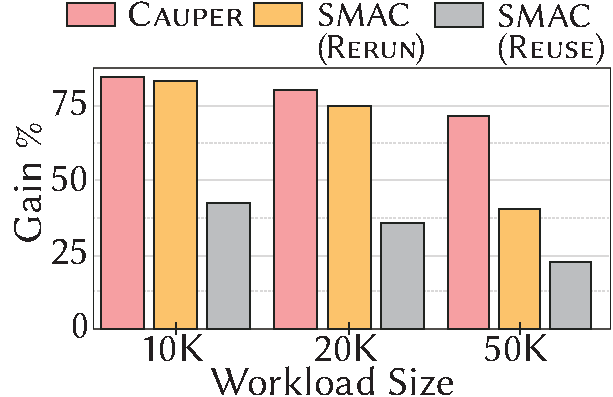
\includegraphics[width=0.45\linewidth]{fig__rq3_d.pdf}
%     \label{fig:rq3_2_a}
%     }~
%     \subfloat[Wallclock time.]{
%         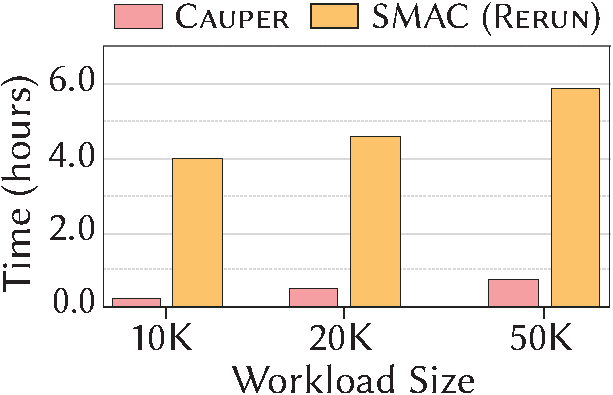
\includegraphics[width=0.45\linewidth]{fig__rq3_e.pdf}
%         \label{fig:rq3_2_b}
%     }
%     \caption{\small \tool vs. SMAC for varying workload. \tool is less sensitive to workload changes.}% (indicated by $\blacklozenge$).}
%     \label{tab:rq3_2}
% \end{figure}

% \motivation
% In this paper, we study fault diagnostic, \ie, situations where a misconfiguration has resulted in non-performance faults, and tools such as  \tool are used to diagnose the root causes and recommend fixes for the misconfiguration. An alternate approach is to use configuration optimization, where the goal is to automatically tune a system by discovering a ``near-optimum'' configuration. 





% \subsubsection*{\textbf{Motivation.}} Search based methods use techniques such as Bayesian optimization~\cite{snoek2012practical, shahriari2015taking} to explore the relationships between configuration options and corresponding non-functional properties. 
% % Unlike machine learning models, optimization methods build and iteratively improve a surrogate model. The balance between exploration (to increase sample diversity) and exploitation (to measure configuration in interesting regions) in the hope of finding a ``near-optimal'' configuration. 
% Albeit recent approaches seem promising~\cite{hsu2018arrow, dalibard2017boat, miyazaki2018bayesian}, these methods are not viable for diagnostics since our objective is not to find an optimal configuration, rather it is to fix an already encountered fault. In this RQ, we explore the challenges of using optimization for fault diagnostics in terms of their efficacy (RQ2-A), their analysis time (RQ2-B), and their sensitivity to external changes (RQ2-C), 
% by comparing \tool with two popular optimization approaches: (a) SMAC and (b) PESMO (see~\tion{baselines}). 


% The assume the software stack to be 
% The prior captures beliefs about the behavior of the function
% decide where to sample to update the 
% model

% to efficiently search the 
% configuration space 

% In this section, we compare \tool with configuration optimization techniques, where the goal is to automatically tune a system by discovering a ``near-optimum'' configuration. Diagnostics (with tools like \tool) and optimization are tangential to one another. Diagnostics fix an already encountered fault, whereas optimization searches the configuration space for a near-optimal configuration. In this section, we contrast the two approaches to understand the challenges of using optimization for fault diagnostics. 

% \approach 
% % \bisq
% % \item \textsc{SMAC}~\cite{hutter2011sequential}: A sequential model based optimization technique to auto-tune software systems; 
% % \item \textsc{PESMO}~\cite{hernandez2016predictive}: A multi-objective bayesian optimization to find an near-optimum configuration.
% % \ei
% % We compare \tool with the following two optimization techniques:
% % 
% % 
% % \besq
% % \item How effective is optimization?
% % % \item How effective is multi-objective optimization?
% % \item What is the analysis time of optimization and \tool?
% % \item How sensitive is optimization to workload changes?
% % % \item Can optimization be used to augment diagnostics?
% % \ee
% % 
% We use latency faults from our benchmark from Image recognition deployed on Jetson \txtwo. There were a total of 21 such faults. Our findings generalize over other combinations of software and hardware.
% 
% 




% \begin{figure}[t]
%     \setlength{\belowcaptionskip}{-1.5em}
%     % \subfloat[\tool vs. SMAC for resolving \\latency faults.]{
%     %     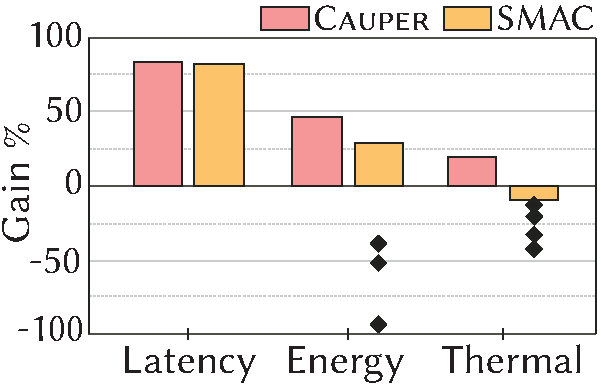
\includegraphics[width=0.3\linewidth]{fig__rq3_a.pdf}
%     %     \label{fig:rq3_1_a}
%     % }\quad
%     \subfloat[\textsc{Xception}]{
%         \includegraphics[width=0.48\linewidth]{figures-vg/Image_sample_energy_gain.pdf}
%         \label{fig:rq2_energy_xception}
%     }
%     % \subfloat[Multi Objective]{
%     %     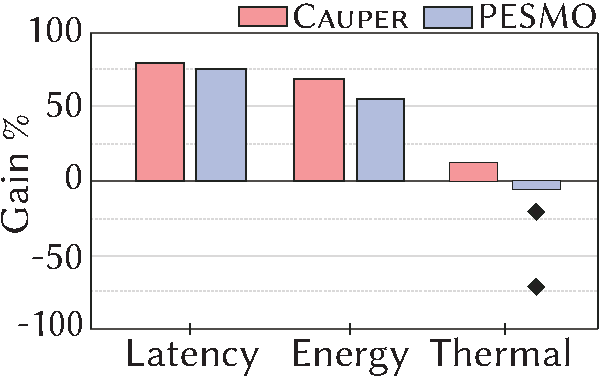
\includegraphics[width=0.275\linewidth]{fig__rq3_b.pdf}
%     %     \label{fig:rq3_1_b}
%     % }
%     \subfloat[\textsc{BERT}]{
%         \includegraphics[width=0.48\linewidth]{figures-vg/NLP_sample_energy_gain.pdf}
%         \label{fig:rq2_energy_bert}
%     }
    
%     \subfloat[\textsc{Deepspeech}]{
%         \includegraphics[width=0.48\linewidth]{figures-vg/Speech_sample_energy_gain.pdf}
%         \label{fig:rq2_energy_deepspeech}
%         }
%         \subfloat[\textsc{x264}]{
%             \includegraphics[width=0.48\linewidth]{figures-vg/x264_sample_energy_gain.pdf}
%             \label{fig:rq2_energy_x264}
%     }
%     \caption{\small{Sample efficiency of \tool in debugging non-functional energy faults}}% (indicated by $\blacklozenge$).}}
%     \label{tab:rq2_2}
% \end{figure}

% \begin{figure*}[t!]
%     % \setlength{\belowcaptionskip}{-3em}
%     \centering
%     \includegraphics*[width=\linewidth]{figures-vg/latency_eff.pdf}
%     \vspace{-3em}
%     \caption{\small{Sample efficiency of \tool in debugging non-functional latency faults}}
    
%     \label{fig:rq2_1}
%     % \rayb{I have questions about this figure. Let's talk in the morning}
% \end{figure*}

% \begin{figure*}[t!]
%     % \setlength{\belowcaptionskip}{-3em}
%     \centering
%     \includegraphics*[width=\linewidth]{figures-vg/energy_eff.pdf}
%     \vspace{-3em}
%     \caption{\small{Sample efficiency of \tool in debugging non-functional energy faults}}
    
%     \label{fig:rq2_2}
%     % \rayb{I have questions about this figure. Let's talk in the morning}
% \end{figure*}
%\subsection{RQ2: How sample efficient is \tool for different performance tasks?}

% \section{Sample Efficiency (RQ2)} 
% % In this RQ, we investigate the sampling efficiency of \tool for different performance tasks. 
% %To answer this RQ, it is sufficient to study \tool for debugging non-functional fault tasks in the SE setting as this generalizes over performance tasks.
% Here, we only study \tool for debugging \textsc{nf-fault} task as this generalizes over performance tasks.

% \noindent \textbf{Setting}.
% We use the same setting for debugging single-objective latency and energy faults for \tool. For other baseline methods, we evaluate the performance gains with varying sample sizes. 

% \noindent \textbf{Results.}
% This issue is compounded when performing multi-objective optimization.% adding to the overall inference time considerably. 

% \tool required a higher number of samples to resolve the latency and energy faults in \textsc{x264} and \textsc{Deepspeech}, respectively when compared to other systems. 
% \bugdoc always achieves a higher gain with the initial 25 number of samples. However, with a higher number of samples, \bugdoc has a slower increase than methods like \textsc{DD} or \textsc{Encore}. 


%~\rayb{Can you explain why causal analysis requires less sample in 1/2 lines?}
\begin{figure}[tp!]
    \setlength{\belowcaptionskip}{-1.5em}
    \centering
    \includegraphics*[width=\linewidth]{figures-vg/barplot_multi_debug_orig.pdf}
    % \includegraphics*[width=0.24\linewidth]{figures-vg/barplot_multi_debug_orig_time.pdf}
    \caption{\small{{\ourapproach has higher accuracy, precision, recall, and gain in debugging non-functional energy faults when hardware changes (\xavier to \txtwo)}}.}% (indicated by $\blacklozenge$).}}
    \label{fig:rq1_debugging_multi}
\end{figure}
% \begin{tcolorbox}
% \textbf{Summary.} \tool is sampling efficient for different performance tasks. 
% \end{tcolorbox}

\begin{figure}[tp!]
    % \setlength{\belowcaptionskip}{-3em}
    \centering
    \includegraphics*[width=\linewidth]{figures-vg/barplot_multi_opt.pdf}
    \caption{\small {\ourapproach finds configurations with higher gain when workloads are changed for performance (latency) optimization task in \txtwo.}}
    
    \label{fig:rq1_opt_me}
    % \rayb{I have questions about this figure. Let's talk in the morning}
\end{figure}

\section{Transferability} 
\label{sec:transfer}

% In this RQ, we investigate the transferability of \tool for different performance tasks. 
%To answer this RQ, it is sufficient to study \tool for debugging non-functional fault task in the SE setting as this generalizes over performance tasks.

% \noindent \textbf{Task1. Debugging \& Repair}.

\noindent \textbf{Setting.} We reuse the causal performance model constructed from a source environment, e.g., \txone, to resolve a non-functional fault in a target environment, e.g., \xavier. We evaluated \ourapproach for debugging energy faults for \textsc{Xception} and used \xavier as the source and \txtwo as the target, since they have different microarchitectures, expecting to see large differences in their performance behaviors. We only compared with \bugdoc as it discovered fixes with higher energy gain in \xavier than other correlation-based baseline methods (see ~\Cref{tab:single_1}). We compared \ourapproach and \bugdoc in the following scenarios: (i) \bugdoc (\textsc{Reuse}) and \ourapproach (\textsc{Reuse}): reusing the recommended configurations from Source to Target, (ii) \bugdoc \textsc{+ 25} and \ourapproach \textsc{+ 25}: reusing the performance models (i.e., causal model and decision tree) learned in Source and fine-tuning the models with 25 new samples in Target, and (iii) \bugdoc (\textsc{Rerun}) and \ourapproach (\textsc{Rerun}): we rerun \ourapproach and \bugdoc from scratch to resolve energy faults in Target. %In both settings, we use relevance score, $\Delta_{gain}$ and wallclock time to determine the effectiveness of \tool. Fig. \ref{fig:acc_shd_iter} indicates how the SCM structure converges to the approximate true causal structure. Here, the structural hamming distance (SHD) value decreases with incremental learning. Fig. \ref{fig:incremental_update} shows how the new recommended configuration from the incremental learning stage resolves the fault and finds the root cause. 
For optimization tasks, we use three larger additional \textsc{Xception} workloads: 10000 (10k), 20000 (20k), and 50000 (50k) test images (previous experiments used 5000 (5k) test images). We evaluated three variants of SMAC and \ourapproach: 
(i)~SMAC (\textsc{Reuse}) and \ourapproach (\textsc{Reuse}), where we \textit{reuse} the near-optimum found with 5k test images on the larger workloads; 
(ii)~SMAC + 10\% and \ourapproach + 10\%, where we rerun with 10\% budget in target and update the optimization and causal performance model with 10\% additional budget; and
(iii)~SMAC + 20\% and \ourapproach + 20\%, where we rerun with 20\% budget in target and update the models with 20\% additional budget.


\noindent \textbf{Results.} 
\fig{rq1_debugging_multi} indicates the results in resolving energy faults in \txtwo. We observe that \ourapproach + 25 obtains 8\% more accuracy, 7\% more precision, 5\% more recall and 8\% more gain than \bugdoc \textsc{(Rerun)}. Here, \bugdoc takes significantly longer time than \ourapproach, \ie, \bugdoc (\textsc{Rerun}) exhausts the entire 4-hour budget whereas \ourapproach takes at most 20 minutes to fix the energy faults. Moreover, we have to rerun \bugdoc every time the hardware changes, and this limits its practical usability. In contrast, \ourapproach incrementally updates the internal causal model with new samples from the newer hardware to learn new relationships. We also observe that with little updates, \ourapproach + 25 ($\sim$20 minutes) achieves a similar performance of \ourapproach \textsc{(Rerun)} ($\sim$36 minutes). Since the causal mechanisms are sparse, the causal performance model from \xavier in \ourapproach quickly reaches a fixed structure in \txtwo using incremental learning by judiciously evaluating the most promising fixes until the fault is resolved.

Our experimental results demonstrate that \ourapproach performs better than the two variants of three SMAC (c.f. \fig{rq1_opt_me}). SMAC (\textsc{Reuse}) performs the worst when the workload changes. With 10K images, reusing the near-optimal configuration from 5K images results in a latency gain of 10\%, compared to 12\% with \ourapproach in comparison with the default configuration. We observe that \ourapproach + 20\% achieves 44\%, 42\%, and 47\% higher gain than SMAC + 20\% for workload sizes of 10k, 20k, and 50k images, respectively. 


% \noindent \textbf{Results}.
% In the earlier RQ, we observed \tool had higher gain and lower hypervolume errors for single and multi-objective optimization, respectively for both settings that can be explained by the results presented in Table. \tool sampled a higher number of better configurations than other approaches and achieved higher gain. Optimization approaches are non-causal and sampled a lower number of configurations as they sampled some costly configurations that had little or no gain. 
% \noindent \textbf{Single-environmental setting results.}
% The analysis time of all approaches are reported in~\fig{rq3_1_c}. Optimization methods run until they converge, however it is a common practice to assign a maximum budget (we use 4 hours) to limit inference time and cost. \tool was found to have comparatively lesser inference time compared to the other methods. While SMAC takes slightly more than 3 hours to find a near-optimum in \txtwo (image recognition), \tool resolved the faults in 20 minutes on average ($9\times$ faster). Likewise, PESMO takes close 4 hours compared to 45 minutes with \tool ($5\times$ faster). 

% \noindent \textbf{Multi-environmental setting results.}
% In \fig{rq3_1_e} we report the inference times for SMAC (\textsc{Rerun}) and \tool. In keeping with the previous results, SMAC (\textsc{Rerun}) takes significantly longer than \tool, \ie, SMAC (\textsc{Rerun}) exceeds the 4 hour budget in all workloads whereas \tool takes at most 30 minutes for the largest workload to diagnose and fix the latency faults. We have to rerun SMAC every time the workload changes, and this limits its practical usability. In contrast, \tool incrementally updates the internal causal model with new samples from the larger workload to learn new relationships from the larger workload. Therefore, it is less sensitive and much faster. 
% Since \tool uses causal models to infer candidate fixes using only the available observational data, it tends to be much faster than SMAC and PESMO. During incremental learning, \tool judiciously evaluates the most promising fixes until the fault is resolved. This limits the number of times the system is reconfigured and profiled. In contrast, optimization techniques sample several sub-optimal configurations in their search process and they are all evaluated. 


% \begin{tcolorbox}
% \textbf{Summary.} \tool is transferable across environments for different performance tasks. 
% \end{tcolorbox}

%\subsection{RQ3: How scalable is \tool for growing configuration spaces for different performance tasks?}

\begin{table}[tp!]
    % \setlength{\belowfloatskip}{-1.5em}
%\caption{Scalability of \tool for \textsc{sqlite} and \textsc{Deepstream} on \xavier.}
\caption{Scalability for \textsc{SQLite} and \textsc{DeepStream} on \xavier.}
\label{tab:scalability}
% \subfloat[Larger number of configuration options.]{
\resizebox{0.98\linewidth}{!}{
\begin{tabular}{V{2}rrrrrrrV{2}rrrV{2}}
\clineB{8-10}{2}
\multicolumn{1}{l}{}              & \multicolumn{1}{l}{}   & \multicolumn{1}{l}{}           &
\multicolumn{1}{l}{}           &
\multicolumn{1}{l}{}           &
\multicolumn{1}{l}{}         & \multicolumn{1}{cV{2}}{}              & \multicolumn{3}{cV{2}}{Time/Fault (in sec.)}                                                    \bigstrut\\ \clineB{1-7}{2}
\multicolumn{1}{V{2}r}{\rotatebox{90}{System}} &{\rotatebox{90}{Configs}}&
{\rotatebox{90}{Events}} &\multicolumn{1}{r}{\rotatebox{90}{Paths}} & \multicolumn{1}{r}{\rotatebox{90}{Queries}} &
\multicolumn{1}{r}{\rotatebox{90}{Degree}} &
\multicolumn{1}{rV{2}}{\rotatebox{90}{Gain (\%)}} & \multicolumn{1}{r}{\rotatebox{90}{Discovery}} & \multicolumn{1}{r}{\rotatebox{90}{Query Eval}} & \multicolumn{1}{rV{2}}{\rotatebox{90}{\bfseries Total}} \bigstrut\\ \hlineB{2}

\multicolumn{1}{c}{}& \multicolumn{1}{c}{}&\multicolumn{1}{c}{}& \multicolumn{1}{c}{}& \multicolumn{1}{c}{}& \multicolumn{1}{c}{}& \multicolumn{1}{c}{}& \multicolumn{1}{c}{}\bigstrut\\[-1.5em] \hlineB{2}

\multicolumn{1}{V{2}r}{\textsc{SQLite}}   & \multicolumn{1}{r}{34}  & \multicolumn{1}{r}{19}                    & \multicolumn{1}{r}{32}        & \multicolumn{1}{r}{191} &   \multicolumn{1}{r}{3.6} & 93                              & 9                            & 14                            & \cellcolor{blue!10}\textbf{291}                     \bigstrut\\ 
\multicolumn{1}{V{2}r}{}    & \multicolumn{1}{r}{242}  & \multicolumn{1}{r}{19}                   & \multicolumn{1}{r}{111}       & \multicolumn{1}{r}{2234}   & \multicolumn{1}{r}{1.9}& 94                               & 57                           & 129                           & \cellcolor{blue!10}\textbf{1345}                    \bigstrut\\
% \multicolumn{1}{V{2}r}{136}                    & \multicolumn{1}{r}{441}       & \multicolumn{1}{r}{8341}    & 93                             & 111                         & 381                             & \cellcolor{blue!10}\textbf{2817}           \bigstrut\\
% \multicolumn{1}{c}{}& \multicolumn{1}{c}{}& \multicolumn{1}{c}{}& \multicolumn{1}{c}{}& \multicolumn{1}{c}{}& \multicolumn{1}{c}{}& \multicolumn{1}{c}{}\bigstrut\\[-1.5em] \hlineB{2}
\multicolumn{1}{V{2}r}{}&  \multicolumn{1}{r}{242} & \multicolumn{1}{r}{288}                      & \multicolumn{1}{r}{441}       & \multicolumn{1}{r}{22372} & \multicolumn{1}{r}{1.6}    & 92                             & 111                         & 854                             & \cellcolor{blue!10}\textbf{5312}           \bigstrut\\ \hlineB{2}
\multicolumn{1}{V{2}r}{\small \textsc{Deepstream}}   & \multicolumn{1}{r}{53}  & \multicolumn{1}{r}{19}                    & \multicolumn{1}{r}{43}        & \multicolumn{1}{r}{497} &   \multicolumn{1}{r}{3.1} & 86                              & 16                            & 32                            & \cellcolor{blue!10}\textbf{1509}                     \bigstrut\\ 

\multicolumn{1}{V{2}r}{}&  \multicolumn{1}{r}{53} & \multicolumn{1}{r}{288}                      & \multicolumn{1}{r}{219}       & \multicolumn{1}{r}{5008} & \multicolumn{1}{r}{2.3}    & 85                             & 97                         & 168                             & \cellcolor{blue!10}\textbf{3113}           \bigstrut\\ \hlineB{2}


\end{tabular}}\vspace{-1em}

\end{table}

\section{Scalability}
\label{sec:scalability}

% Scalability of \tool depends on the scalability of each phase. Therefore, we design scenarios to test the scalability of each phase to determine the overall scalability. Since the initial number of samples and the underlying phases for each task is the same, it is sufficient to examine the scalability of \tool for the debugging non-functional fault task. 

 
% \textsc{sqlite} was chosen because it offers a large number of configurable options, much more than  DNN-based applications, and video encoders. Further, each of these options can take on a large number of permitted values making \textsc{Deepstream} a useful candidate to study the scalability of \tool. \textsc{Deepstream} was chosen as it has a higher number of components than others and it is interesting to determine how \tool behaves when the number of options and events are increasing.
% As a result, SQLite exposes new system design opportunities to enable efficient inference and many complex interactions between software options. 
% We evaluate \tool under two scalability scenarios: (1) larger configuration space (RQ3-A), and (2) more granular values for each configuration option (RQ3-B). 

% \noindent\textbf{RQ3-A.~How does \tool scale with a larger number of configuration options?} 
\noindent{\textbf{Setting.}}~ We evaluated \ourapproach for scalability with \textsc{SQLite} (large configuration space) and \textsc{Deepstream} (large composed system). %The causal graphs of DNN based systems used 47 variables with 34 hardware, kernel/OS, and software configuration options in addition to 19 system events.
In \textsc{SQLite}, we evaluated three scenarios: (a)~selecting the most relevant software, hardware options, and events (34 configuration options and 19 system events), (b) selecting all modifiable software and hardware options and system events (242 configuration options and 19 events), and (c) selecting not only all modifiable software and hardware options and system events but also intermediate {\tt tracepoint events} (242 configuration options and 288 events). In \textsc{Deepstream}, there are two scenarios: (a) 53 configuration options and 19 system events, and (b) 53 configuration options and 288 events when we select all modifiable software and hardware options, and system/tracepoint events. %For each scenario, we track the time required to discover the causal structure, evaluate the counterfactual queries, and total time to resolve throughput faults. 


\noindent{\textbf{Results.}} In large systems, there are significantly more causal paths and therefore, causal learning and estimations of queries take more time. %However, with as much as 242 configuration options and 19 events (\tab{scalability}, row 2), causal graph discovery takes roughly one minute, evaluating all 2234 queries takes roughly two minutes, and the total time to diagnose and fix a fault is roughly 22 minutes for \textsc{sqlite}. This trend is observed even with 242 configuration options, 288 events (\tab{scalability}, row 3), and finer granularity of configuration values---the time required to causal model recovery is a little over 1 minute and the total time to diagnose and fix a fault is less than 2 hours. Similarly in \textsc{Deepstream}, with 53 configuration options and 288 events, causal model discovery is less than two minutes and the time needed to diagnose and fix a fault is less than an hour. 
The results in ~\tab{scalability} indicate that \ourapproach can scale to a much larger configuration space without an exponential increase in runtime for any of the intermediate stages. This can be attributed to the sparsity of the causal graph. For example, the average degree of a node for \textsc{SQLite} in \tab{scalability} is at most 3.6, and it reduces to 1.6 when the number of configurations increases. Similarly, the average degree reduces from 3.1 to 2.3 in \textsc{Deepstream} when systems events are increased. %This makes sense because not all variables (\ie, configuration options and/or system events) affect non-functional properties and a high number of variables in the graph end up as isolated nodes. Therefore, the number of paths and consequently the evaluation time do not grow exponentially as the number of variables increases.

% To understand how \tool scales in such scenarios, we evaluate \tool by increasing the number of values the software, hardware, and kernel configuration options can be set to while resolving the latency faults in the SQLite. From \tab{scalability} we observe that even with 242 configurations, 288 events (\tab{scalability}, row 3), and finer granularity of configuration values, the time required to causal model recovery is less than two minutes and the total time to diagnose and fix a fault is less than 2 hours. We also observe that the graph becomes more sparse (average degree of a node decreases from 1.8 to 1.6 in \tab{scalability}) and the evaluation time does not grow exponentially. 

% Finally, the latency gain associated with repairs from larger configuration space with configurations was similar to the original space of 34 and 53 configurations for \textsc{sqlite} and \textsc{Deepstream}, respectively. This indicates that: (a)~imparting domain expertise to select most important configuration options can speed up the inference time of \tool, and (b)~if the user chooses instead to use more configuration options (perhaps to avoid initial feature engineering), \tool can still diagnose and fix faults %satisfactorily within a reasonable time. 

% To understand how \tool scales in such scenarios, we evaluate \tool by increasing the number of values the software, hardware, and kernel configuration options can be set to while resolving the latency faults in the SQLite. %There are two scenarios in this case: (a) 242 configurations and 88 system events when we select all the modifiable software/hardware configurations and events and (b) 242 configurations and 288 events when we select not only all modifiable software and hardware configurations and system events but also intermediate {\tt tracepoint events}. 
% In the second case, we increase the granularity of kernel configurations by considering all the permitted values by \texttt{Linux} kernel. As system events can only be observed, we increase the granularity of events by observing the tracepoint events along with hardware/software events. 
% Similar to {RQ3-A.}, we track the time required to discover the causal structure, evaluate the counterfactual queries, and total time to resolve latency faults.
% 


% In summary, 

% x
\section{Related Work}
\label{sec:related}
\noindent
% \textbf{Performance modeling.} Understanding performance behavior is critical to detect root causes of non-functional faults. Black-box performance influence models \cite{siegmund2015performance,krishna2019conex, krishna2020whence,dorn2020generating,dornmastering} as well as white-box performance analysis \cite{velez2019configcrusher} have been employed to understand performance behaviour of systems. Transfer learning strategies had been adopted to alleviate the complexity of learning performance behavior across environments, e.g., model transfer across hardware \cite{jamshidi2017transfer,iqbal2019transfer,javidian2019transfer}. However, these methods cannot be used to diagnose non-functional faults as they cannot be used to answer debugging queries.

\noindent\textbf{Performance faults in configurable systems.} Previous empirical studies have shown that a majority of performance issues are due to misconfigurations~\cite{han2016empirical}, with severe consequences in production environments~\cite{tang2015holistic,maurer2015fail}, and configuration options that cause such performance faults force the users to tune the systems themselves~\cite{zhang2021evolutionary}. Previous works have used static and dynamic program analysis to identify the influence of configuration options on performance~\cite{VJSSAK:ASE20,velez2021white,li2020statically} and to detect and diagnose misconfigurations~\cite{XJHZLJP:OSDI16,attariyan2010automating,zhang2013automated,attariyan2012x}. 
Unlike \ourapproach, none of the white-box analysis approaches target configuration space across the system stack, where it limits their applicability in identifying the true causes of a performance fault. 

% However, the configuration options keep increasing over time~\cite{xu2015hey} and make the configuration-aware testing a difficult endeavor, where testing can be only practical by evaluating a representative sample of all possible configurations~\cite{qu2008configuration}, by employing sampling strategies to discover potential (performance) faults~\cite{medeiros2016comparison}. 




% Researchers have studied performance degradations due to misconfigurations using different sampling~\cite{medeiros2016comparison} and static empirical approaches~\cite{han2016empirical, mordahl2019empirical, li2020statically}. \textsc{SyncProf}~\cite{yu2016syncprof, yu2018pinpointing} develops an end-to-end technique to detect performance bugs and optimize performance bottlenecks in configurable systems. Several performance analysis and debugging approaches have been proposed for detecting structured workflows using noisy logs \cite{wu2017structural}, anomaly diagnosis \cite{jia2017approach, wang2015data}, and data-driven approaches~\cite{yu2018understanding, curtsinger2012stabilizer,curtsinger2016effective}. Due to heavy reliance on the data, these methods are significantly costly and cannot be used to detect misconfigurations arising due to non-functional faults.

% \noindent\textbf{Performance Modeling and Optimization.}
% % Performance behavior of configurable systems is complex (non-linear, non-convex, and multi-modal)~\cite{wang2018understanding,jamshidi2016uncertainty}, where such behavior becomes even more intricate when multiple objectives are needed to be traded-off for performance-related tasks~\cite{kolesnikov2019tradeoffs,nardi2019hypermapper,iqbal2020flexibo}. 
% A common strategy to understand complex performance behavior is to use machine-learning by building a black-box model that characterizes system performance~\cite{siegmund2015performance,valov2017transferring,guo2013variability}. The learned performance model can then be used for performance debugging ~\cite{siegmund2015performance,guo2013variability,wang2018understanding} and tuning~\cite{H:AS}.
% % While the sheer size of the configuration space and complex performance behavior prohibit any guarantee of finding a globally optimal configuration, 
% Optimization algorithms attempt to find near-optimal configurations under a limited sampling budget using a clever combination of sampling, model construction, and search. Several methods have been attempted including hill climbing~\cite{XLRXZ:WWW04}, optimization via guessing~\cite{OK:SIGMETRICS07}, Bayesian optimization~\cite{JC:MASCOTS16}, and multi-objective optimization~\cite{wu2015deep,iqbal2020flexibo}. 
% % However, if one of the contextual/environmental conditions (e.g., hardware, workload) of the system changes, one needs to rerun the optimization approach again~\cite{JVKS:FSE18}, therefore, transfer learning in terms of transferring measurement data or extracting some types of knowledge across environments has been used~\cite{valov2017transferring,JSVKPA:ASE17,JVKSK:SEAMS17,javidian2019transfer,iqbal2019transfer,krishna2019whence,valov2020transferring}. 
% % For a more comprehensive treatment of the literature, we refer to~\cite{pereira2019learning,siegmund2020dimensions}.
% Although black-box models have been used extensively for optimization, they cannot diagnose non-functional faults as they are unaware of underlying causal factors due to their blind exploration without having access to the underlying causal relationships.

\noindent\textbf{Statistical and model-based debugging.}
Debugging approaches such as \textsc{Statistical Debugging}~\cite{song2014statistical}, 
\textsc{HOLMES}~\cite{chilimbi2009holmes}, \textsc{XTREE}~\cite{krishna2017less}, \bugdoc~\cite{lourencco2020bugdoc}, \encore~\cite{lourencco2020bugdoc}, \textsc{Rex}~\cite{mehta2020rex}, and \textsc{PerfLearner}~\cite{han2018perflearner} have been proposed to detect root causes of system faults. These methods make use of statistical diagnosis and pattern mining to rank the probable causes based on their likelihood of being the root causes of faults. However, these approaches may produce correlated predicates that lead to incorrect explanations.

% cannot provide any contextual information regarding how the root causes lead to faults and are costly as they require running expensive experiments for acquiring reliable performance measurements. 

% Methods like \textsc{Caramel}~\cite{nistor2015caramel} and \textsc{Toddler}~\cite{nistor2013toddler} use similarity analysis to detect performance bugs with non-intrusive fixes. These methods rely on the conditions and loops present in the source code to fix a bug; therefore, cannot be extended to debug misconfigurations. 

\noindent\textbf{Causal testing and profiling.} 
Causal inference has been used for fault localization \cite{baah2010causal,feyzi2019inforence}, resource allocations in cloud systems~ \cite{geiger2016causal}, and causal effect estimation for advertisement recommendation systems \cite{bottou2013counterfactual}. More recently, \textsc{AID}~\cite{fariha2020causality} detects root causes of an intermittent software failure using fault injection as an intervention. \textsc{Causal Testing} ~\cite{johnson2020causal} modifies the system inputs to observe behavioral changes and utilizes counterfactual reasoning to find the root causes of bugs. Causal profiling approaches like \textsc{CoZ}~\cite{curtsinger2015coz} point to developers where optimizations will improve performance and quantify their potential impact. Causal inference methods like \textsc{X-Ray}~\cite{attariyan2012x} and \textsc{ConfAid}~\cite{attariyan2010automating} had previously been applied to analyze program failures. All approaches above are either orthogonal or complementary to \ourapproach, mostly they focus on functional bugs (e.g., \textsc{Causal Testing}) or if they are performance-related, they are not configuration-aware (e.g., \textsc{CoZ}). 

% \noindent\textbf{Design Space Exploration (Systems and Architecture).} TODO: add references in arch community around DSE

% Both \textsc{AID} and \textsc{Causal Testing} are orthogonal to \tool as they aim to identify intermittent and functional bugs. 


% A causal profiler conducts a series of performance experiments to empirically observe the effect of potential optimization. These methods use virtual speedups to mimic the effect of optimizing a specific line of code by a fixed amount. However, to detect and fix misconfigurations as the developers do not have direct access to the source code. Therefore, these methods cannot be used directly to observe the optimization effects. \tool is targeted for highly-configurable systems, and the root causes of misconfigurations result due to complex interactions across the system stack. 

% \textsc{Inforence}~\cite{feyzi2019inforence} have also used statistical causal inference on observational data for software fault localization. These approaches are suitable to detect faults in a program but cannot be applied to detect non-functional faults as the workflow of developing a program dependency graph is absent due to not having access to the program source code. 






%Therefore, we develop \tool to identify the root causes of non-functional faults in configurable systems. 

%  Researchers have also developed techniques to automate analyses using \textsc{Differential Slicing}~\cite{johnson2011differential}. Differential slicing outputs a causal difference graph that captures the differences of input that triggered the observed difference and the causal path of differences that led from those input differences to the observed difference. These methods aim towards discovering the causal path of execution differences but require a complete program execution trace generated by execution indexing. \textsc{Dual slicing}~\cite{weeratunge2010analyzing} is another program slicing-based technique to discover statement-level causal paths for concurrent program failures. These program slicing-based approaches only consider two executions—one successful and one failed. These approaches are white-box where the developer of the system intends to discover the root cause of the fault. \tool is used in scenarios where the user experiences a performance issue and intends to fix it by changing configuration across the system stack. For performance debugging, it might not be possible to know about the successful executions (more performant configurations) in advance.  
 %had also been proposed 
 
%  In the context of performance debugging, these temporal relationships are not valid; hence, cannot be used to detect root causes. 

% \noindent\textbf{Explanation-centric approaches.}
% Explanation-centric approaches like explanation tables \cite{el2014interpretable} and query-based diagnosis \cite{wang2017qfix} are relevant to \tool as they aim at generating explanations for certain outcomes (faults). However, these methods do not allow to perform interventions which makes them less useful for detecting the root cause of performance faults.

 


% \noindent\textbf{Fault Localization and Tuning.} Causal profiling approaches like \textsc{Coz}~\cite{curtsinger2015coz} guides developers to code where optimizations will improve program performance. A causal profiler conducts a
% series of performance experiments to empirically observe the effect of potential optimization. These methods use virtual speedups to mimic the effect of optimizing a specific line of code by a fixed amount. However, to detect and fix misconfigurations as the developers do not have direct access to the source code. Therefore, these methods cannot be used directly to observe the optimization effects. \tool is targeted for highly-configurable systems, and the root causes of misconfigurations result due to complex interactions across the system stack. Causal inference methods like \textsc{X-Ray}~\cite{attariyan2012x} and \textsc{ConfAid}~\cite{attariyan2010automating} had previously been applied to analyze program failures using run-time control and data flow behavior. \textsc{Inforence}~\cite{feyzi2019inforence} have also used statistical causal inference on observational data for software fault localization. These approaches are suitable to detect faults in a program but cannot be applied to detect non-functional faults as the workflow of developing a program dependency graph is absent due to not having access to the program source code. 


% Encore\cite{zhang2014encore}\rayb{???}

% \noindent\textbf{Fault injection}. Fault injection techniques~\cite{alvaro2015lineage,marinescu2009lfi} intervene application runtime behavior with the goal to test if an application can handle
% the injected faults. In fault injection techniques, faults to be
% injected are chosen based on whether they can occur in practice.
% However, in performance debugging faults resulting due to misconfigurations, cannot be known in advance. 

% \noindent\textbf{Group testing}. Group testing~\cite{bai2019adaptive, agarwal2018novel, li2014group}  has been applied for fault diagnosis. Specifically, adaptive group testing is related to the interventions performed in \tool. However, none of
% the existing works consider the scenario where a group test might
% reveal additional information and thus offers an inefficient solution
% for causal path discovery.

% \noindent\textbf{Control flow graph}. Control flow graph-based techniques~\cite{cheng2009identifying, jiang2007context} aims at identifying bug signatures for sequential programs using discriminative
% subgraphs within the program’s control flow graph; or generating
% faulty control flow paths that link many bug predictors. But these
% approaches cannot be extended to detect misconfigurations as they do not consider causal connection among and program failure.


\section{Limitations and Future Directions}
\label{sec:discussion}


\noindent \textbf{Learning a predictive model vs learning the underlying structure.}
Building a causal performance model could be more expensive than performance influence models. The reason for having a potentially higher learning cost is that in addition to learning a predictive model, we also need to learn the structure of the input configuration space.
However, exploiting causal knowledge is more helpful in search-like tasks (e.g., performance optimization~\cite{JC:MASCOTS16,JVKS:FSE18}) that looks for %searching through the search space that finds 
higher quality samples, making it possible to debug or optimize with a few samples.

\noindent \textbf{Dealing with an incomplete causal model.} Existing off-the-shelf causal graph discovery algorithms like FCI remain ambiguous while data is insufficient and returns partially directed edges. For highly configurable systems, gathering high-quality data is challenging. To address this issue, we develop a novel pipeline for causal model discovery by combining FCI with entropic causality, an information-theoretic approach~\cite{Kocaoglu2017} to causality that takes the direction across which the entropy is lower as the causal direction. Such an approach helps to reduce ambiguity and thus allows the causal graph to converge faster. Note that estimating a theoretical guarantee for convergence is out of scope, as having a global view of the entire configuration space is infeasible. Moreover,  the presence of too many confounders can affect the correctness of the causal models, and this error may propagate along with the structure if the dimensionality is high. Therefore, we use a greedy refinement strategy to update the causal graph incrementally with more samples; at each step, the resultant graph can be approximate and incomplete, but asymptotically, it will be refined to its correct form given enough time and samples.

\noindent \textbf{Algorithmic innovations for faster convergence.} The efficacy of \ourapproach depends on several factors such as the representativeness of the observational data or the presence of unmeasured confounders that can negatively affect the quality of the causal model. There are instances where the causal model may be incorrect or lack some crucial connections that may result in detecting spurious root causes or recommending incorrect repairs. One promising direction to address this problem would be to develop new algorithms for Stage II \& III of \ourapproach (see Section~\ref{sec:methodology}). Specifically, we see the potential for developing innovative approaches for learning better structure, incorporating domain knowledge by restricting the structure of the underlying causal model. In addition, there are potentials for developing better sampling algorithms by either shrinking the search space (e.g., using transfer learning~\cite{JVKS:FSE18}) or searching the space more efficiently to determine effective interventions that enable faster convergence to the true underlying structure. 

\noindent \textbf{Incorporating domain knowledge.} Additionally, there is scope for developing new approaches for either automatically extracting constraints (e.g., from source code or other downstream artifacts) to incorporate in learning causal performance model or approaches to make humans part of the loop for correcting the causal performance model during learning. Specifically, new approaches could provide infrastructure as well as algorithms to determine when to ask for human feedback and what to ask for, e.g., feedback regarding a specific part of the causal model or feedback regarding the determined intervention at each step.

\noindent \textbf{Developing new domain-specific languages.} \ourapproach uses a query engine to translate common user queries into counterfactual statements. A domain-specific language to facilitate automated specification of queries from written unstructured data could potentially lead to the adoption of causal reasoning in the system development lifecycle. 
\section{Conclusion}
\label{sect:conclusion}

Modern computer systems are highly-configurable with thousands of interacting configurations with a complex performance behavior. Misconfigurations in these systems can elicit complex interactions between software and hardware configuration options, resulting in non-functional faults. We propose \ourapproach, a novel approach for diagnostics that learns and exploits the system's causal structure consisting of configuration options, system events, and performance metrics. Our evaluation shows that \ourapproach effectively and quickly diagnoses the root cause of non-functional faults and recommends high-quality repairs to mitigate these faults. We also show that the learned causal performance model is transferable across different workload and deployment environments. Finally, we demonstrate the scalability of \ourapproach scales to large systems consisting of 500 options and several trillion potential configurations. 

%l\ourapproach's code is released at \url{https://github.com/softsys4ai/unicorn}.

%The experimental results are promising for performance optimization.


% \section*{Acknowledgements} We like to thank Christian K$\ddot{\text{a}} $stner, Sven Apel, Yuriy Brun, Emery Berger, Tianyin Xu, Vivek Nair, Jianhai Su, Miguel Velez, Tobius D$\ddot{\text{u}}$rschmid for their valuable feedback and suggestions in improving the paper. This work was partially supported by NASA (RASPBERRY-SI Grant Number 80NSSC20K1720) and NSF (SmartSight Award 2007202). 

\section*{Acknowledgements} This work has been supported in part by NASA (Awards 80NSSC20K1720 and 521418-SC) and NSF (Awards 2007202, 2107463, and 2038080), Google, and Chameleon Cloud. We are grateful to all who provided feedback on this work, including Christian K$\ddot{\text{a}} $stner, Sven Apel, Yuriy Brun, Emery Berger, Tianyin Xu, Vivek Nair, Jianhai Su, Miguel Velez, Tobius D$\ddot{\text{u}}$rschmid, and the anonymous EuroSys'22 (as well as EuroSys'21 and FSE'21) reviewers. 

%\section{Scalability of \tool}

To examine the scalability of \tool, we evaluate \tool using the speedtest workload of SQLite database to resolve the latency faults due to misconfigurations. SQLite database workloads have a higher number of configurable options compared to image, NLP, and speech workloads. SQLite workloads exhibit unique compute, memory, data reuse characteristics, and higher memory accesses. As a result, SQLite exposes new system design opportunities to enable efficient inference and many complex interactions between software options. We evaluate \tool on the following two scenarios:

\noindent\paragraph{Increasing number of configuration options.} In the first scenario, we perform a sensitivity analysis of \tool by increasing the size of the configuration space. We start with 47 configuration options which we manually select based on important hardware, kernel configuration options, and system events recommended in performance blogs. Then we increase the number of configuration options to 330 by including 206 \texttt{sysctl} kernel configuration options that can be tuned without rebooting the system. Finally, we extend the number of configuration options to 530 by including all the system events tracked by \textsc{iperf}. In each case, we track the time required to discover the causal structure, evaluate the counterfactual queries and resolve a latency fault.  

\noindent\paragraph{Increasing number of configuration options' values.} \tool recommends a fix by computing individual treatment effect to evaluate counterfactual queries. The number of these counterfactual queries depends on the number of values taken by a configuration option. If a configuration option can be set to a large number of values, the number of counterfactual queries needed to be evaluated also increases. To determine the behavior of \tool in such scenarios, we evaluate \tool by increasing the number of values the hardware and kernel configuration options can be set at while resolving the latency faults in the SQLite speedtest workload. 

% references section

\bibliographystyle{acm}
\balance
\bibliography{references,bib_pjamshidi}
\clearpage 
\balance
\appendix
.%%%%%%%%%%%%%%%%%%%%%%%%%%%%%%%%%%%%%%%%%%%%%%%%%%%%
% Artifact Appendix Template for EuroSys'22 AE
%
% this document has a maximum length of 2 pages.
%%%%%%%%%%%%%%%%%%%%%%%%%%%%%%%%%%%%%%%%%%%%%%%%%%%%

% \appendix
%%%%%%%%%%%%%%%%%%%%%%%%%%%%%%%%%%%%%%%%%%%%%%%%%%%%%%%%%%%%%%%%%%%%%

\section{Artifact Appendix}
\label{sec:artifact}
\begin{tcolorbox}[colback=blue!5!white,colframe=blue!75!black]
\textbf{DOI:} \url{doi:10.5281/zenodo.6360540} \\
\textbf{Code:} \url{https://github.com/softsys4ai/unicorn}
\end{tcolorbox}

This appendix provides additional information regarding the tool that we have developed for evaluating \ourapproach. In this section, we call this tool \ourtool. In addition, we describe the steps using our \ourtool to reproduce the results reported in \S\ref{sec:effectiveness}, \S\ref{sec:transfer}, and \S\ref{sec:scalability}. We provide the source code and data in a publicly accessible GitHub repository that can be tested on any hardware once the software dependencies are met. 

\subsection{Description}
\ourapproach is used for performing tasks such as performance optimization and performance debugging in both offline and online modes. 
\begin{itemize}
    \item In the offline mode, \ourtool can be run on any device that uses previously measured configurations.
    \item In the online mode, the performance metrics are measured directly on the hardware on which the underlying configurable system is deployed, while the experiments are running. In the experiments, we have used \txtwo and \xavier. To collect measurements from these devices, \emph{sudo} privilege is needed, as it requires setting a device to a new configuration before measurement.
\end{itemize}
%  In both offline and online modes, \ourtool can be used for debugging and optimization for objectives such as latency and energy. 
 
%  \ourapproach has been implemented on six software systems such as \textsc{Deepstream} (Deepstream), \textsc{Xception} (Image), \textsc{Bert} (NLP), \textsc{Deepspeech} (Speech), \textsc{x264} (x264), and \textsc{sqlite} (sqlite).

% \subsection{Access}
% Our repository can be accessed online with the following link: \href{unicorn}{https://github.com/softsys4ai/unicorn}.

\subsection{Setup}


% \begin{tcolorbox}[colback=blue!5!white,colframe=blue!75!black]
% \textsc{NVIDIA Jetson Xavier}
%   \tcblower
% \textsc{Processor}: 6-core ARM CPU, 8 MB L2 + 4 MB L3

% \textsc{GPU}: 384-core Volta GPU with 48 Tensor cores

% \textsc{Memory}: 8 GB 256-bit LPDDR4x 1333MHz

% \textsc{Jetpack}: 4.3 \textsc{OS}: Ubuntu 20.04 64-bit
% \end{tcolorbox}
% \begin{tcolorbox}[colback=blue!5!white,colframe=blue!75!black]
% \textsc{NVIDIA Jetson TX2}
% \tcblower
% \textsc{Processor}: Dual-core NVIDIA Denver 2 64-bit CPU and quad-core Arm Cortex-A57 

% \textsc{GPU}: NVIDIA Pascal arch. with 256 CUDA cores

% \textsc{Memory}: 4 GB 128-bit LPDDR4 51.2 GB/s

% \textsc{Jetpack}: 4.3 \textsc{OS}: Ubuntu 20.04 64-bit
% \end{tcolorbox}

\subsubsection{Software Dependencies}
\ourtool is implement-ed by integrating and building on top of several existing tools (see \fig{unicorn-toolchain}): 
\begin{itemize}
    \item \href{https://semopy.com/}{\color{blue!80}semopy} for predictions with causal models.
    \item \href{https://ananke.readthedocs.io/en/latest/}{\color{blue!80}ananke} and \href{https://github.com/akelleh/causality}{\color{blue!80}causality} for estimating the causal effects.
    \item \href{https://github.com/cmu-phil/causal-learn}{\color{blue!80}causal-learn} for structure learning. 
\end{itemize}


\subsubsection{Hardware Dependencies}
\ourtool is implemented both in offline and online modes. There are no particular hardware dependencies to run \ourtool in offline mode. To run \ourtool in online mode, we used hardware that has sensors for performance measurements. In particular, we used \txone, \txtwo, and \xavier with \emph{Jetpack 4.3} and \emph{Ubuntu 20.04 LTS}.

\subsubsection{Installation}
We use \textit{docker-compose} to install the necessary software required to run \ourtool. The necessary steps to install the dependencies and third-party libraries used to test our approach can be done with the following commands.

\begin{verbatim}
git clone git@github.com:softsys4ai/unicorn.git
cd unicorn
docker-compose up --build --detach
\end{verbatim}


\begin{figure}[hb!]
    \centering
    \includegraphics[width=\linewidth]{figures-vg/UnicornTool.pdf}
    \caption{Toolchain in \ourtool.}
    \label{fig:unicorn-toolchain}
\end{figure}

Once this step is completed, \ourtool is ready to be tested.


\subsection{Data} 
All the datasets required to run experiments are already included in the \textit{./unicorn/data} directory.  

\subsection{Major Claims}
We make the following major claims in our paper:
\begin{itemize}
\item \ourapproach can be used to detect root causes of non-functional performance (latency and energy) faults with higher accuracy and gain.

\item \ourapproach can support performing downstream performance tasks such as performance optimization.

\item The causal performance models are transferable across environments (different workload or hardware) and can be efficiently re-used from the source environment where it is trained to a target environment.
\end{itemize}

\subsection{Experiments}
We run the following experiments to support our claims.

\subsubsection{E1: Performance Debugging Experiment} To support the claim of efficiency of \ourapproach in debugging non-functional faults, we reproduce energy faults results for \textsc{Xception} in \textsc{Nvidia Jeston Xavier} from Table~\ref{tab:single_1}. Our initial study discovered 29 energy faults for \textsc{Xception} in \textsc{Nvidia Jetson Xavier,} that is 12\% of the faults reported in Table~\ref{tab:single_1}. This would require ~1.5 hours to run the experiments in offline mode and ~11 hours to run the experiments in online mode.

\noindent\textbf{Execution}. To run \ourtool on a single bug, execute the following command:

\begin{verbatim}
docker-compose exec unicorn python \\ 
./tests/run_unicorn_debug.py -o \\
total_energy_consumption -s Image -k Xavier \\
-m offline\online -i 0
\end{verbatim}

To run \ourtool and other debugging baselines reported in this paper on all the bugs, please use the following commands one by one:
\begin{verbatim}
docker-compose exec unicorn python \\ 
./tests/run_unicorn_debug.py -o \\
total_energy_consumption -s Image -k Xavier \\
-m offline\online 
    
docker-compose exec unicorn python \\ 
./tests/run_baseline_debug.py -o \\
total_energy_consumption -s Image -k Xavier \\
-m offline\online -b cbi 
    
docker-compose exec unicorn python \\ 
./tests/run_baseline_debug.py -o \\
total_energy_consumption -s Image -k Xavier \\
-m offline\online -b encore
    
docker-compose exec unicorn python \\ 
./tests/run_baseline_debug.py -o \\
total_energy_consumption -s Image -k Xavier \\
-m offline\online -b bugdoc
    
\end{verbatim}

\noindent \textbf{Results}. We save the evaluation metrics such as accuracy, precision, recall, gain, and time required for debugging. A separate plot is generated using the recommended fixes to compare \ourapproach with other baseline approaches with their evaluation metrics. Note, in the offline mode the reported time is different (usually less) from the main text as instead of running the measurements online we reuse recorded measurements. However, we can get a sense of the efficiency by comparing the number of samples required to resolve a fault.

\subsubsection{E2: Performance Optimization Experiment} \ourapproach supports can support performing downstream performance tasks such as performance optimization. To support this claim, we reproduce single-objective latency optimization results reported in \fig{rq1_opt_se} (a). This experiment would require around ~1.5 hours to complete in the offline mode and ~4 hours to complete in the online mode. We also compare the results with a baseline optimization approach, \textsc{SMAC}, reported in the paper. 


\noindent \textbf{Execution}. To run the experiment, we need to execute the following commands:

\begin{verbatim}
docker-compose exec unicorn python \\ 
./tests/run_unicorn_optimization.py -o \\
inference_time -s Image -k TX2 \\
-m offline\online 
    
docker-compose exec unicorn python \\ 
./tests/run_baseline_optimization.py -o \\
inference_time -s Image -k TX2 \\
-m offline\online -b smac
\end{verbatim}

\noindent \textbf{Results}. We display the results similar to \fig{rq1_opt_se} (a) using a line plot. Note that this experiment is run once without repeating, so there are no error bars.

\subsubsection{E3: Transferability Experiment.} To support this claim, we initially build a causal performance model to resolve the latency faults in \xavier and reuse the causal performance model to resolve the latency faults in \txtwo. We only use one bug to demonstrate this result. This would require ~10 minutes to run the experiment in the offline mode and ~25 minutes in the online mode. 

\noindent \textbf{Execution}. The following command runs the experiments:

\begin{verbatim}
docker-compose exec unicorn python \\ 
./tests/run_unicorn_transferability.py -o \\
inference_time -s Image -k Xavier \\
-m offline\online 

\end{verbatim}

\noindent \textbf{Results}. The evaluation metrics, including accuracy, precision, recall, gain, and time required for debugging for different scenarios reported in the paper are saved to a separate CSV file after the experiments are over and plotted. Note that the reported time is different from the time reported in the main text in the offline mode. 

\subsection{Using \ourtool with external data}
We added \href{https://github.com/softsys4ai/unicorn/blob/master/artifact/OTHERS.md}{\color{blue!80}instructions} to describe the required steps to use \ourtool with any other external dataset.

\subsection{Extending \ourtool}
We welcome any contribution for extending either \ourapproach (see \S\ref{sec:discussion} for several possible future directions) and \ourtool for performance improvements or feature extensions.  


%%%%%%%%%%%%%%%%%%%%%%%%%%%%%%%%%%%%%%%%%%%%%%%%%%%%%%%%%%%%%%%%%%%%%
\clearpage
\section{Appendix}
\label{sec:appendix}
\subsection{Causal Performance Modeling and Analyses: Motivating Scenarios (Additional details)}




\fig{spurious_two} and ~\fig{spurious_three} present additional scenarios where performance influence models could produce incorrect explanations. The regression terms presented here incorrectly identify spurious correlations, whereas the causal model correctly identifies the cause-effect relationships. 



The performance behavior of regression models for configurable systems varies when sample size varies. ~\fig{reg_eq_noise} shows the change of a number of stable terms and error with different numbers of samples used for building a performance influence model. Here, we vary the number of samples from 50 to 1500 to build a source regression model. We use a sample size of 2000 to build the target regression model. We observe that regression models cannot be reliably used in performance tasks, as they are sensitive to the number of training samples. The results indicate that these model classes as opposed to causal models cannot identify causal variables underlying system performance, so depending on the training sample, they try to find the best predictor to increase the prediction power with the i.i.d. assumption that does not hold in system performance. On the contrary, the number of stable predictor's variation is less in causal performance models and leads to better generalization, as shown in ~\fig{reg_eq_noise_cpm}. In addition to the number of stable predictors, the difference in error between source and target is negligible when compared to the performance regression models. 

\begin{figure}[h]
\small
    % \setlength{\belowcaptionskip}{-3em}
    \centering
    \includegraphics*[width=0.5\linewidth]{figures-vg/spurious_two.pdf}
    \caption{\small {Performance influence model incorrectly identifies \texttt{Batch Size} and \texttt{QoS} are positively correlated with the term $\texttt{0.08 Batch Size} \times \texttt{QoS}$ whereas they are unconditionally independent. Causal model correctly identifies the dependence (no causal connection) relationship between \texttt{Batch Size} and \texttt{QoS} (no arrow between \texttt{Batch Size} and \texttt{QoS})}.}
    \label{fig:spurious_two}
    
\end{figure}
\begin{figure}[h]
\small
    % \setlength{\belowcaptionskip}{-3em}
    \centering
    \includegraphics*[width=0.7\linewidth]{figures-vg/spurious_three.pdf}
    \caption{\small {Causal model correctly identifies how \texttt{CPU Frequency} causally influences \texttt{Throughput} via \texttt{Cycles} whereas the performance influence model $\texttt{Throughput} = 0.05 \times \texttt{CPU Frequency} \times \texttt{Cycles}$ identified incorrect interactions. }}
    \label{fig:spurious_three}
    
\end{figure}





\noindent \textbf{Extraction of predictor terms from the causal performance model.} The constructed causal performance models have performance objective nodes at the bottom (leaf nodes) and configuration options nodes at the top level. The intermediate levels are filled with the system events. To extract a causal term from the causal model, we backtrack starting from the performance objective until we reach a configuration option. If there is more than one path through a system event from performance objective to configuration options, we consider all possible interactions between those configuration options to calculate the number of causal terms.


\begin{figure}[h]
\small
    % \setlength{\belowcaptionskip}{-3em}
    \centering
    \includegraphics*[width=\linewidth]{figures-vg/reg_eq_noise.pdf}
    \caption{\small {Performance influence models relying on correlational statistics are not stable as new samples are added and do not generalize well. Common terms refers to the individual predictors (i.e., options and interactions) in the performance models that are similar across envirnments.}}
    \label{fig:reg_eq_noise}
    
\end{figure}

\begin{figure}[h]
\small
    % \setlength{\belowcaptionskip}{-3em}
    \centering
    \includegraphics*[width=\linewidth]{figures-vg/reg_eq_noise_cpm.pdf}
    \caption{\small {Causal performance models are relatively more stable as new samples are added and do generalize well.}}
    \label{fig:reg_eq_noise_cpm}
    
\end{figure}

\subsection{\ourapproach (Additional details)}

Note, if $X$ is a continuous variable, we would replace the summation of $ACE$ with an integral. 
% 
% \eq{ace} represents the average causal effect over a pair of nodes in a path. 
For the entire path, we extend it as:
\smalleq
\label{eq:path_ace}
{\footnotesize
\setlength{\abovedisplayskip}{1pt}
\setlength{\belowdisplayskip}{1pt}
\mathrm{Path}_{ACE} = \frac{1}{K} \cdot \sum \mathrm{ACE}(Z, X) \hspace{2em} \footnotesize \forall X, Z \in path 
}
\eeq
\eq{path_ace} represents the average causal effect of the causal path. The configuration options that lie in paths with larger $P_{ACE}$ tend to have a greater causal effect on the corresponding non-functional properties in those paths. We select the top $K$ paths with the largest $\mathrm{P}_{ACE}$ values, for each non-functional property. In this paper, we use K=3 to 25, however, this may be modified in our replication package. 

% \noindent\textbf{\textsl{Aside.}}~In eqs.~\ref{eq:do} and~\ref{eq:ace}, $\mathbb{E}(Y~|~do(X=x))$ is \textit{not} the same as the ordinary conditional distribution $\mathbb{E}\left(Y~|~X=x\right)$. This is because $\mathbb{E}\left(Y~|~X=x\right)$ takes the original population, as is, and filters it get the sub-population where $X=x$. If $X=x$ does not exist in the population, the value of $\mathbb{E}\left(Y~|~X=x\right)$ would be misleading. In contrast, $\mathbb{E}\left(Y~|~\mathit{do}\left(X=x\right)\right)$ uses do-calculus rules~\cite{pearl2009causality} to infer the value of the distribution even when $X=x$ has never been encountered before. 

\begin{table}[]
\centering
\caption{Mapping between configuration options and options indexes. Only a subset of configuration options are shown here.}
\resizebox{\linewidth}{!}{
\begin{tabular}{llll}
\hline
Option&Configuration& Option& Configuration\\
Index & Options & Index & Options\\
\hline
0& \texttt{Swap Memory} &14& \texttt{kernel.numa\_balancing}  \\
1& \texttt{Scheduler Policy}&15& \texttt{kernel.sched\_latency\_ns} \\
2&\texttt{Drop Caches}&16& \texttt{kernel.sched\_nr\_migrate} \\
3& \texttt{Batch Size}& 17& \texttt{kernel.sched\_rt\_period\_us} \\
4& \texttt{Bitrate}&18& \texttt{kernel.sched\_rt\_runtime\_us}\\
5& \texttt{Buffer Size} &19& \texttt{kernel.sched\_time\_avg\_ms}\\
6& \texttt{CPU Freqeuncy}&20& \texttt{kernel.sched\_child\_runs\_first}\\
7& \texttt{GPU Frequency}& 21& \texttt{vm.vfs\_cache\_pressure} \\
8& \texttt{EMC Frequency}& 22& \texttt{vm.swappiness}\\
9& \texttt{CPU Cores}& 23& \texttt{Enable Padding}\\
10& \texttt{vm.overcommit\_memory}& 24& \texttt{vm.dirty\_background\_ratio}\\
11& \texttt{vm.overcommit\_hugepages}& 25& \texttt{vm.dirty\_background\_bytes}\\
12& \texttt{kernel.cpu\_time\_max\_percent}& 26& \texttt{vm.dirty\_ratio}\\
13& \texttt{kernel.max\_pids}& 27& \texttt{vm.nr\_hugepages}\\
\hline
\end{tabular}}
\label{tab:mapping}
\end{table}


\begin{table}[]
\centering
\caption{Configuration options in \textsc{Xception}, \textsc{Bert}, and \textsc{Deepspeech}.}
\begin{tabular}{lll}
\hline
Configuration Options & Option Values/Range  \\
\hline 
\texttt{Memory Growth}                      &    -1, 0.5, 0.9            \\ 
\texttt{Logical Devices}                      &  0, 1               \\ 
\hline
\end{tabular}
\label{tab:ml_conf}
\end{table}


\begin{table}[]
\centering
\caption{\textsc{x264} software configuration options.}
\begin{tabular}{lll}
\hline
Configuration Options & Option Values/Range  \\
\hline 
\texttt{CRF} &  13, 18, 24, 30               \\  
\texttt{Bit Rate} & 1000, 2000, 2800, 5000         \\  
\texttt{Buffer Size} &  6000, 8000, 20000          \\  
\texttt{Presets} &   ultrafast, veryfast, faster\\
& medium, slower  \\  
\texttt{Maximum Rate} &       600k, 1000k         \\  
\texttt{Refresh} &       OFF, ON         \\  
\hline
\end{tabular}
\label{tab:x264_conf}
\end{table}


\begin{table}[]
\centering
\caption{\textsc{SQLite} software configuration options.}
\resizebox{\linewidth}{!}{\begin{tabular}{lll}
\hline
Configuration Options & Option Values/Range \\
\hline 
\texttt{PRAGMA TEMP\_STORE}           &   DEFAULT, FILE, MEMORY              \\  
\texttt{PRAGMA JOURNAL\_MODE}           &      DELETE, TRUNCATE,PERSIST,MEMORY, OFF          \\  
\texttt{PRAGMA SYNCHRONOUS}           &    FULL, NORMAL, OFF          \\  
\texttt{PRAGMA LOCKING\_MODE}           &     NORMAL, EXCLUSIVE            \\  
\texttt{PRAGMA CACHE\_SIZE}           &    0, 1000, 2000, 4000, 10000             \\ 
\texttt{PRAGMA PAGE\_SIZE}           &   2048, 4096, 8192         \\ 
\texttt{PRAGMA MAX\_PAGE\_COUNT}           &   32, 64            \\ 
\texttt{PRAGMA MMAP\_SIZE}           &  30000000000, 60000000000,\\
\hline
\end{tabular}}
\label{tab:sqlite_conf}
\end{table}


\begin{table}[]
\centering
\caption{Linux OS/Kernel configuration options.}
\resizebox{\linewidth}{!}{
\begin{tabular}{lll}
\hline
Configuration Options & Option Values/Range  \\
\hline 
\texttt{vm.vfs\_cache\_pressure}& 1, 100, 500                 \\  
\texttt{vm.swappiness} &  10, 60, 90\\
\texttt{vm.dirty\_bytes} &30, 60\\
\texttt{vm.dirty\_background\_ratio}&10, 80\\
\texttt{vm.dirty\_background\_bytes}&30, 60\\
\texttt{vm.dirty\_ratio}&5, 50\\
\texttt{vm.nr\_hugepages}&0, 1, 2\\
\texttt{vm.overcommit\_ratio}&50, 80\\
\texttt{vm.overcommit\_memory}&0, 2\\
\texttt{vm.overcommit\_hugepages}&0, 1, 2\\
\texttt{kernel.cpu\_time\_max\_percent}&10 - 100\\
\texttt{kernel.max\_pids}&32768, 65536\\
\texttt{kernel.numa\_balancing} &0, 1\\
\texttt{kernel.sched\_latency\_ns} &24000000, 48000000\\
\texttt{kernel.sched\_nr\_migrate} &32, 64, 128\\
\texttt{kernel.sched\_rt\_period\_us} &1000000, 2000000&\\
\texttt{kernel.sched\_rt\_runtime\_us} &500000, 950000\\
\texttt{kernel.sched\_time\_avg\_ms} &1000, 2000\\
\texttt{kernel.sched\_child\_runs\_first} &0, 1&\\
\texttt{Swap Memory}&1, 2, 3, 4 (GB)\\
\texttt{Scheduler Policy}&CFP, NOOP\\
\texttt{Drop Caches}&0, 1, 2, 3\\


\hline
\end{tabular}}
\label{tab:os_conf}
\end{table}

\begin{table}[]
\centering
\caption{Hardware configuration options.}
\begin{tabular}{lll}
\hline
Configuration Options & Option Values/Range \\
\hline 
\texttt{CPU Cores}           &   1 - 4              \\
\texttt{CPU Frequency}           &  0.3 - 2.0 (GHz)              \\
\texttt{GPU Frequency}           &  0.1 - 1.3 (GHz)               \\
\texttt{EMC Frequency}           &  0.1 - 1.8 (GHz)               \\
\hline
\end{tabular}
\label{tab:hw_conf}
\end{table}

\begin{table}[]
\centering
\caption{Performance system events and tracepoints. }
\begin{tabular}{lll}
\hline
System Events \\
\hline 
\texttt{Context Switches}\\ 
\texttt{Major Faults}         \\ 
\texttt{Minor Faults }                              \\ 
\texttt{Migrations}                           \\ 
\texttt{Scheduler Wait Time}                             \\ 
\texttt{Scheduler Sleep Time}                             \\ 
\texttt{Cycles}                               \\
\texttt{Instructions}                             \\ 
\texttt{Number of Syscall Enter}                       \\ 
\texttt{Number of Syscall Exit}                       \\ 
\texttt{L1 dcache Load Misses}            \\                   
\texttt{L1 dcache Loads}                               \\
\texttt{L1 dcache Stores}                               \\
\texttt{Branch Loads}                               \\
\texttt{Branch Loads Misses}                            \\
\texttt{Branch Misses}                            \\
\texttt{Cache References}\\
\texttt{Cache Misses}\\
\texttt{Emulation Faults}                               \\
% Alignment faults \\
\hline
Tracepoint Subsystems\\
\hline
\texttt{Block}\\
\texttt{Scheduler}\\
\texttt{IRQ}\\
\texttt{ext4}\\
\hline
\end{tabular}
\label{tab:event_conf}
\end{table}


% \subsubsection{Phase-III: Counterfactual Query Evaluation}
% \label{sect:root_cause}
Counterfactual queries can be different for different tasks. For debugging, we use the top $K$ paths to (a)~identify the root cause of non-functional faults; and (b)~prescribe ways to fix the non-functional faults. Similarly, we use the top $K$ paths to identify the options that can improve the non-functional property values near-optimal.
% \subsubsection{Translating developer's queries into counterfactual statements}
For both tasks, a developer may ask specific queries to \ourapproach and expect an actionable response. For debugging, we use the example causal graph of where a developer observes low FPS and high energy, \ie, a multi-objective fault, and has the following questions:  %We use this example to answer some of the developer's questions: 

\noindent\textbf{\faQuestionCircle~\textbf{``What are the root causes of my multi-objective (\texttt{FPS} and \texttt{Energy}) fault?''}} To identify the root cause of a non-functional fault, we must identify which configuration options have the most causal effect on the performance objective. %For example, in the causal graph of~\fig{path_eg}, we are required to find which of the configuration options $X_1, X_2, Z_1, Z_2$ has the highest causal effect on $Y$. 
For this, we use the steps outlined in~\tion{path_discovery} to extract the paths from the causal graph and rank the paths based on their average causal effect (\ie, $\mathrm{Path}_{ACE}$ from \eq{path_ace}) on latency and energy. We return the configurations that lie on the top $K$ paths. 
For example, in ~\fig{causal_model_example} we may return (say) the following paths: 
\bisq
\small
    \item  \texttt{Batch Size} \edgeone \texttt{Cache Misses} \edgeone \texttt{FPS} and \texttt{Energy}
    \item  \texttt{Enable Padding}  \edgeone \texttt{Cache Misses}  \edgeone \texttt{FPS} and \texttt{Energy}
\ei
 
% \item \cpufreq~\edgeone \swapmem \edgeone Latency,
and the configuration options {\texttt{BatchSize}, and \texttt{Enable Padding}} being the probable root causes.

\noindent\textbf{\faQuestionCircle~\textbf{``How to improve my \texttt{FPS} and \texttt{Energy}?''}} To answer this query, we first find the root causes as described above. Next, we discover what values each of the configuration options must take in order that the new \texttt{FPS} and \texttt{Energy} is better (high \texttt{FPS} and low \texttt{Energy}) than the fault (low \texttt{FPS} and high \texttt{Energy}). For example, we consider the causal path \texttt{Batch Size}~\edgeone \texttt{Cache Misses} \edgeone \texttt{FPS} and \texttt{Energy}, we identify the permitted values for the configuration options {\texttt{Batch Size}} that can result in a high FPS and energy ($Y^{\mathit{\textsc{low}}}$) that is better than the fault ($Y^{\mathit{\textsc{high}}}$).
For this, we formulate the following counterfactual expression: 
\smalleq
\label{eq:cfact_bare}
\footnotesize
\mathrm{Pr}(Y_{repair}^{\textsc{low}}|\neg repair,Y_{\neg repair}^{\textsc{high}})
\eeq
\eq{cfact_bare} measures the probability of ``fixing'' the latency fault with a ``repair'' {\footnotesize $(Y_{repair}^{\textsc{low}})$} given that with no repair {we observed the fault} {\footnotesize $(Y_{\neg repair}^{\text{\textsc{high}}})$}.   
In our example, the repairs would resemble \texttt{Batch Size}=$10$. We generate a \textit{repair set} ($\mathcal{R}_{1}$), where the configurations \texttt{Batch Size} is set to all permissible values, \ie,
{
\small
\begin{multline}\label{eq:repairs}
    \setlength{\abovedisplayskip}{5pt}
    \setlength{\belowdisplayskip}{5pt}
    \mathcal{R}_{1}\equiv~\bigcup~\left\{\texttt{Batch Size} = {x},... \right\}\forall {x} \in \texttt{Batch Size}
\end{multline}}
observe that, in the repair set ($\mathcal{R}_{1}$) a configuration option that is not on the path \texttt{Batch Size}~\edgeone \texttt{Cache Misses} \edgeone \texttt{FPS} and \texttt{Energy} is set to the same value of the fault. For example, \texttt{Bit Rate} is set to $2$ or \texttt{Enable Padding} is set to $1$. This way we can reason about the effect of interactions between \texttt{Batch Size} with other options, i.e., \texttt{Bit Rate}, \texttt{Buffer Size}. Say \texttt{Buffer Size} or \texttt{Enable padding} were changed/recommended to set at any other value than the fault in some previous iteration, i.e., $20$ or $0$, respectively. In that case, we set \texttt{BufferSize} and \texttt{Enable padding}=$0$. Similarly, we generate a repair set $\mathcal{R}_{2}$ by setting \texttt{Enable Padding}to all permissible values. 
{
\small
\begin{multline}\label{eq:repairs}
    \setlength{\abovedisplayskip}{5pt}
    \setlength{\belowdisplayskip}{5pt}
    \mathcal{R}_{2}\equiv~\bigcup~\left\{\texttt{Enable padding} = {x},... \right\} \forall {x} \in \texttt{Enable padding}
\end{multline}}


Now, we combine the repair set for each path to construct a final repair set $\mathcal{R}=\mathcal{R}_{1} \cup~\ldots \cup\mathcal{R}_{k}$. Next, we compute the \textit{Individual Causal Effect} (ICE) on the \texttt{FPS} and \texttt{Energy} ($Y$) for each repair in the repair set $\mathcal{R}$. In our case, for each repair $\mathit{r}~\in~\mathcal{R}$, ICE is given by:
\begin{equation}
    \label{eq:ite}
    \footnotesize
    \mathrm{ICE}(\mathit{r})=\mathrm{Pr}(Y_r^{\textsc{low}}~|~\neg r,~Y_{\neg r}^{\textsc{high}}) - \mathrm{Pr}(Y_r^{\textsc{high}}~|~\neg r,~Y_{\neg r}^{\textsc{high}})\hspace{1em}
\end{equation}
ICE measures the difference between the probability that \texttt{FPS} and \texttt{Energy} \textit{is low} after a repair $r$ and the probability that the \texttt{FPS} and \texttt{Energy} is \textit{still high} after a repair $r$. If this difference is positive, then the repair has a higher chance of fixing the fault. In contrast, if the difference is negative, then that repair will likely worsen both \texttt{FPS} and \texttt{Energy}. To find the most useful repair ($\mathcal{R}_{\mathit{best}}$), we find a repair with the largest (positive) ICE, \ie, $\mathcal{R}_{\mathit{best}} = \argmax_{\forall r~\in~\mathcal{R}}[\mathrm{ICE}(\mathit{r})]$. This provides the developer with a possible repair for the configuration options that can fix the multi-objective \texttt{FPS} and \texttt{Energy} fault. 


% The above formulation can be extended to accommodate queries that involve multiple non-functional properties (\eg, improve \textit{both} latency and energy consumption). To do this, we may reformulate \eq{ite} to compute the probability that a repair $r$ can reduce both latency ($Y_r^{\textsc{low}}$) and the energy consumption ($W_r^{\textsc{low}}$), \ie,
% {
% \small
% \begin{multline}\label{eq:repairs_2}
%     \setlength{\abovedisplayskip}{5pt}
%     \setlength{\belowdisplayskip}{5pt}
%     \mathrm{ITE}(\mathit{r})=\mathrm{Pr}(Y_r^{\textsc{low}}, W_r^{\textsc{low}}~|~\neg r,~Y_{\neg r}^{\textsc{high}},~W_{\neg r}^{\textsc{high}}) \\ -~\mathrm{Pr}(Y_r^{\textsc{high}}, W_r^{\textsc{high}}~|~\neg r,~Y_{\neg r}^{\textsc{high}},~W_{\neg r}^{\textsc{high}})
% \end{multline}}
% \noindent\hspace{-3pt}After, computing \eq{repairs_2}, we can find a repair $r$ with the largest (positive) ITE as per~\eq{best_intervention}. 
% \begin{equation}
%     \label{eq:ite}
%     \footnotesize
%     \mathrm{ITE}(\mathit{r})=\mathrm{Pr}(Y_r^{\textsc{low}}, W_r^{\textsc{low}}~|~\neg r,~Y_{\neg r}^{\textsc{high}},~W_{\neg r}^{\textsc{high}}) - \mathrm{Pr}(Y_r^{\textsc{high}}~|~\neg r,~Y_{\neg r}^{\textsc{low}})\hspace{1em}
% \end{equation}

% \[\bigcup\limits_{{x_1} \in {X_1},{x_2} \in {X_2},...} {P(Y = {y_{fixed}}|do({X_1} = {x_1},{X_2} = {x_2},...))} \]

% \noindent\textbf{\faQuestionCircle~\textbf{``How to decrease my latency using the same energy consumption''}} There queries involve multiple non-functional properties (in this case, latency and energy consumption). 
% % An example, let us try to minimize latency without affecting energy consumption. 
% We enumerate all possible repairs as counterfactual statements as per~\eq{repairs}. Next, we compute the \textit{individual treatment effect} (ITE) for each repair in three steps: 
% \besq
% \item  
% {\footnotesize$\mathrm{P_{fix}}=\mathrm{Pr}(Y_r^\textsc{low},~W_r^\textsc{same}~|~\neg r,W_{\neg r}^\textsc{same}, Y_{\neg r}^\textsc{high} )$}.
% \item Compute the probability that a repair $r$ \textit{cannot} fix the latency (\ie, $Y^{\text{\textsc{high}}}$) or it actually worsens energy consumption (\ie, $W^{\text{\textsc{high}}}$), \ie, {\footnotesize$\mathrm{P_{no~fix}}=\mathrm{Pr}(W_r^\textsc{high},~Y_r^\textsc{high} ~|~\neg r,W_{\neg r}^\textsc{high}, Y_{\neg r}^\textsc{high})$}.
% \item Finally, compute the $ITE(\mathit{r})$ as {$
% \footnotesize \mathrm{ITE}(\mathit{r})=\mathrm{P_{fix}} - \mathrm{P_{no~fix}}$}
% \ee

% If this difference is large, then the repair `$r$' has a high likelihood of fixing the latency fault in $Y^\text{\textsc{high}}$ while keeping the energy consumption $W^\text{\textsc{high}}$ unchanged.  We find the best repair operator with the highest $ITE(\mathit{r})$ using~\eq{best_intervention}. 

\noindent \textbf{Remarks.}~The ICE computation of \eq{ite} occurs \textit{only} on the observational data. Therefore, we may generate any number of repairs and reason about them without having to deploy those interventions and measure their performance in the real world. This offers significant runtime benefits.

\subsection{Evaluation (Additional details)}

\subsubsection{Experimental setup}

\label{subsec:experimental_setup}
\begin{table}[]
\centering
\caption{Deepstream software configuration options.}
\resizebox{\linewidth}{!}{
\begin{tabular}{llll}
\hline
Component&Configuration Options & Option Values/Range  \\
\hline 
&\texttt{CRF} &  13, 18, 24, 30               \\  
&\texttt{Bitrate} & 1000, 2000, 2800, 5000         \\  
&\texttt{Buffer Size} &  6000, 8000, 20000          \\  
Decoder&\texttt{Presets} &   ultrafast, veryfast, faster\\
&& medium, slower  \\  
&\texttt{Maximum Rate} &       600k, 1000k         \\  
&\texttt{Refresh} &       OFF, ON         \\  
\hline
&\texttt{Batch Size} &       0 - 30         \\  
&\texttt{Batched Push Timeout}&  0 - 20           \\  
&\texttt{Num Surfaces per Frame} & 1, 2, 3, 4\\
Stream Mux&\texttt{Enable Padding} & 0, 1          \\  
&\texttt{Buffer Pool Size} &  1 - 26               \\  
&\texttt{Sync Inputs} &  0, 1          \\ 
&\texttt{Nvbuf Memory Type} &     0, 1, 2, 3         \\ 
\hline
&\texttt{Net Scale Factor} &  0.01 - 10              \\  
&\texttt{Batch Size}& 1 - 60                \\  
&\texttt{Interval} &  1 - 20               \\  
&\texttt{Offset} &       0, 1          \\  
Nvinfer&\texttt{Process Mode} &   0, 1              \\ 
&\texttt{Use DLA Core} &      0, 1           \\ 
&\texttt{Enable DLA} &           0, 1      \\ 
&\texttt{Enable DBSCAN} &       0, 1       \\ 
&\texttt{Secondary Reinfer Interval} &       0 - 20          \\ 
&\texttt{Maintain Aspect Ratio} &       0, 1          \\ 
\hline
&\texttt{IOU Threshold} &       0 - 60          \\
&\texttt{Enable Batch Process} &       0, 1          \\
Nvtracker&\texttt{Enable Past Frame} &       0, 1          \\
&\texttt{Compute HW} &       0, 1, 2, 3, 4          \\ 
\hline
\end{tabular}}
\label{tab:deepstream_conf}
\end{table}

We used the following four components for Deepstream implementation:

\begin{itemize}
\item \textbf{Decoder}: For the decoder, we use x264. It uses the x264 and takes the encoded H.64, VP8, VP9 streams, and produces an NV12 stream.

\item \textbf{Stream Mux}:
The streammux module takes the NV12 stream and outputs the NV12 batched buffer with information about input frames, including the original timestamp and frame number.

\item \textbf{Nvinfer}:
For object detection and classification, we use the TrafficCamNet model that uses ResNet 18 architecture. This model is pre-trained in 4 classes on a dataset of 150k frames and has an accuracy of 83.5\% for detecting and tracking cars from a traffic camera's viewpoint. The 4 classes are Vehicle, BiCycle, Person, and Roadsign. We use the Keras (Tensorflow backend) pre-trained model from TensorRT.


\item \textbf{Nvtracker}:
The plugin accepts NV12- or RGBA-formated frame data from the upstream component and scales (converts) the input buffer to a buffer in the format required by the low-level library, with tracker width and height. NvDCF tracker uses a correlation filter-based online discriminative learning algorithm as a visual object tracker while using a data association algorithm for multi-object tracking. 
\end{itemize}

\noindent \textbf{Configuration options, events, and hyperparameters used for evaluation.}
Table~\ref{tab:deepstream_conf}, Table~\ref{tab:ml_conf}, Table~\ref{tab:x264_conf}, and Table~\ref{tab:sqlite_conf}, show different software configuration options and their values for different systems considered in this paper. Table~\ref{tab:os_conf} shows the OS/kernel level configuration options and their values for different systems considered in this paper. Additionally, Table~\ref{tab:event_conf}
shows the performance events considered in this paper. The hyperparameters considered for \textsc{Xception}, \textsc{Bert}, and \textsc{Deepspeech} are shown in Table~\ref{tab:dnn_conf}.


\begin{table}[]
\centering
\caption{Hyperparameters for DNNs used in \ourapproach.}
\resizebox{\linewidth}{!}{\begin{tabular}{lll}
\hline
Architecture & Hyperparameters & Option Values\\
\hline 
&\texttt{Number of Filters Entry} flow &32 \\
&\texttt{Filter Size Entry Flow} &(3 $\times$ 3)\\
&\texttt{Number of Filters Middle Flow} &64 \\
&\texttt{Filter Size Middle Flow} &(3 $\times$ 3)\\
\textsc{Xception}&\texttt{Number of Filters Exit Flow} &728\\
&\texttt{Filter Size Exit Flow} &(3 $\times$ 3)\\
&\texttt{Batch Size} &32\\
&\texttt{Number of Epochs}&100\\
\hline
&\texttt{Dropout} & 0.3\\
&\texttt{Maximum Batch Size}&16\\
\textsc{Bert}&\texttt{Maximum Sequence Length}&13\\
&\texttt{Learning Rate} &$1e^{-4}$\\
&\texttt{Weight Decay} &0.3\\
\hline
&\texttt{Dropout} & 0.3\\
&\texttt{Maximum Batch Size}& 16\\
\textsc{Deepspeech}&\texttt{Maximum Sequence Length}&32\\
&\texttt{Learning Rate} &$1e^{-4}$\\
&\texttt{Number of Epochs}&10\\
\hline
\end{tabular}}
\label{tab:dnn_conf}
\end{table}

% \begin{figure}
%     \centering
%     \includegraphics[width=\linewidth]{figures-vg/lineplot_multienv.pdf}
%     \caption{Ranking of configurations may change across environments, here between two hardware (\xavier and \txtwo). The reason can be associated with differences in microarchitecture and different hardware resources.}
%     \label{fig:multi_env_change}
% \end{figure}

% Causal performance models capture the underlying causal mechanisms and use them for performance-related tasks in the new environments. On the other hand, performance influence models need to relearn the patterns from scratch, therefore, they demand more samples in the new environments.
\begin{table}[]
\centering
\caption{Hyperparameters for FCI used in \ourapproach.}
\begin{tabular}{lll}
\hline
Hyperparameters & Value \\
\hline 
\texttt{depth} &-1 \\
\texttt{testId} &fisher-z-test\\
\texttt{maxPathLength} &-1 \\
\texttt{completeRuleSetUsed}&False\\
\hline 

\end{tabular}
\end{table}
% % \begin{table*}[h]
% \caption{\small Configurations options by each layer.}
% \small 
% \resizebox{\linewidth}{!}{\begin{tabular}[t]{p{0.35\linewidth}|p{0.3\linewidth}p{0.2\linewidth}p{0.2\linewidth}p{0.2\linewidth}}
 
% \centering
% Configuration options& & Layer&\\
% \midrule
% \multicolumn{5}{c}{Workload}\\
% \cmidrule(lr){1-5}\\ 
% &\multicolumn{4}{c}{DNN}\\
% \cmidrule(lr){2-5}\\
% Memory growth & 0, 0.1, 0.5&\\
% Logical devices & 10, 50\\ 
% \cmidrule(lr){2-5}\\
% &\multicolumn{4}{c}{SQLite}\\
% \cmidrule(lr){2-5}\\
% Cache size & 0, 0.1, 0.5&\\
% Buffer size & 10, 50\\ 
% Synchronous & 0, 1 \\
% Journal mode & Memory, Disk \\
% Temporary store & Memory, Disk \\

% \cmidrule(lr){2-5}\\
% &\multicolumn{4}{c}{x264}\\
% \cmidrule(lr){2-5}\\
% CRF & 0, 0.1, 0.5&\\
% Preset & 10, 50\\
% Bit rate & 10,100\\
% Latency & 1,2 \\
% \hline 
% \multicolumn{5}{c}{OS/Kernel}\\
% \cmidrule{1-5}\\
% Scheduler policy& CFP, NOOP\\
% Swappiness&10, 60, 100\\
% Dirty background ratio&10, 80\\
% Dirty ratio& 5, 50\\
% Sched child runs first & 0, 1 \\
% Drop caches & 0, 1, 2, 3\\
% Cache pressure & 1, 100, 500 \\

% \hline
% \multicolumn{5}{c}{Hardware}\\
% \cmidrule{1-5}\\
% & \multicolumn{1}{l}{\nano}&\multicolumn{1}{l}{\txone} & \multicolumn{1}{l}{\txtwo} & \multicolumn{1}{l}{\xavier}\\
% \cmidrule{2-2}\cmidrule{3-3}\cmidrule{4-4}\cmidrule{5-5}\\
% Active CPUs&1 - 4&1 - 4&1 - 4&1 - 4\\
% CPU freq. (GHz)&0.3 - 2.0&0.3 - 2.0&0.3 - 2.0&0.3 - 2.0\\
% GPU freq. (GHz)& 0.1 - 1.3&0.3 - 2.0&0.3 - 2.0&0.3 - 2.0\\
% EMC freq. (GHz)&0.1 - 1.8&0.3 - 2.0&0.3 - 2.0&0.3 - 2.0\\

% \bottomrule
% \end{tabular}}
% \label{tab:configurations}
% \end{table*}%}




\subsubsection{Case Study.}
~\fig{real_wrold_cpm} shows the causal graph to resolve the real-world latency fault.

\begin{figure}[t!]
\small
    % \setlength{\belowcaptionskip}{-3em}
    \centering
    \includegraphics*[width=\linewidth]{figures-vg/fig__realworld.pdf}
    \caption{\small {Causal graph used to resolve the latency fault in the real world case study in section~\ref{sec:casestudy}}}
    \label{fig:real_wrold_cpm}
    
\end{figure}

\begin{table*}[h]
    \centering
    \caption{\small  Efficiency of \ourapproach compared to other approaches. Cells highlighted in \colorbox{blue!10}{\bfseries blue} indicate improvement over faults and \colorbox[HTML]{FFCCC9}{red} indicate deterioration. \ourapproach achieves better performance overall and is much faster.
    }
\vspace{-0.85em}
\subfloat[Single objective performance fault for \textit{heat} in \txone.]{\scriptsize
    \label{tab:rq1_1}
    \resizebox{\textwidth}{!}{
    \begin{tabular}{@{}l|l|l|lllll|lllll|lllll|lllll|ll|}
        \clineB{4-25}{2}
        \multicolumn{1}{c}{}&\multicolumn{1}{c}{}  &  & \multicolumn{5}{c|}{Accuracy} & \multicolumn{5}{c|}{Precision} & \multicolumn{5}{c|}{Recall} & \multicolumn{5}{c|}{Gain} & \multicolumn{2}{c|}{Time$^\dagger$} \bigstrut\\ \clineB{4-25}{2}
        \multicolumn{1}{c}{}& \multicolumn{1}{c}{} &  & \multicolumn{1}{c}{\rotatebox{90}{\bfseries \ourapproach}} &
        \multicolumn{1}{c}{\rotatebox{90}{\cbi}} & \multicolumn{1}{c}{\rotatebox{90}{DD}} & \multicolumn{1}{c}{\rotatebox{90}{\encore}} & \multicolumn{1}{c|}{\rotatebox{90}{\bugdoc~}} & \multicolumn{1}{c}{\rotatebox{90}{\bfseries \ourapproach}} &  
        \multicolumn{1}{c}{\rotatebox{90}{\cbi}} & \multicolumn{1}{c}{\rotatebox{90}{DD}} & \multicolumn{1}{c}{\rotatebox{90}{\encore}} & \multicolumn{1}{c|}{\rotatebox{90}{\bugdoc~}} & \multicolumn{1}{c}{\rotatebox{90}{\bfseries \ourapproach}} &
        \multicolumn{1}{c}{\rotatebox{90}{\cbi}} & \multicolumn{1}{c}{\rotatebox{90}{DD}} & \multicolumn{1}{c}{\rotatebox{90}{\encore}} & \multicolumn{1}{c|}{\rotatebox{90}{\bugdoc~}} & \multicolumn{1}{c}{\rotatebox{90}{\bfseries \ourapproach}} & \multicolumn{1}{c}{\rotatebox{90}{\cbi}} & \multicolumn{1}{c}{\rotatebox{90}{DD}} & \multicolumn{1}{c}{\rotatebox{90}{\encore}} & \multicolumn{1}{c|}{\rotatebox{90}{\bugdoc
        ~}} & \multicolumn{1}{c}{\rotatebox{90}{\bfseries \ourapproach}} &  \multicolumn{1}{c|}{\rotatebox{90}{Others}} \bigstrut[t]
        \\ \clineB{4-25}{2}
    \multicolumn{1}{c}{}&\multicolumn{1}{c}{}  & \multicolumn{1}{c}{} & \multicolumn{1}{c}{} & \multicolumn{1}{c}{} & \multicolumn{1}{c}{} & \multicolumn{1}{c}{} & \multicolumn{1}{c}{} \bigstrut\\[-1.4em]\hlineB{2}
    
     &  & \textsc{Xception} & \cellcolor{blue!10}\bfseries69 & 63 & 57 & 64 & 65 & \cellcolor{blue!10}\bfseries 75 & 56 & 56 & 60 & 66 & \cellcolor{blue!10}\bfseries68  & 62 & 58 & 64 & 69 & \cellcolor{blue!10}\bfseries4  & 3 & 2 & 2 & 3 & \cellcolor{blue!10}\bfseries0.6 &4 \\
     
     &  & \textsc{BERT} & \cellcolor{blue!10}\bfseries71 &62 & 61 & 61 & 62 & \cellcolor{blue!10}\bfseries72  & 56 & 59 & 56 & 61 & \cellcolor{blue!10}\bfseries 72 & 65 & 62 & 67 & 62 & \cellcolor{blue!10}\bfseries5  & 3 & 2 & 2 & 3 & \cellcolor{blue!10}\bfseries0.4 & 4 \\
     
     &  & \textsc{Deepspeech} & \cellcolor{blue!10}\bfseries71  & 61 & 64 & 62 & 67 & \cellcolor{blue!10}\bfseries71  & 58 & 59 & 54 & 68 & \cellcolor{blue!10}\bfseries69  & 67 & 66 & 68 & 67 & \cellcolor{blue!10}\bfseries3 & 3 & 2 & 2 & 2 & \cellcolor{blue!10}\bfseries0.7  & 4 \\
     
     & \multirow{-4}{*}{\rotatebox{90}{Heat}} & \textsc{x264} & \cellcolor{blue!10}\bfseries74  & 65 & 57 & 64 & 65 & \cellcolor{blue!10}\bfseries74  &62 & 54 & 55 & 65 & \cellcolor{blue!10}\bfseries74 & 66 & 63 & 68 & 69 & \cellcolor{blue!10}\bfseries7  & 3 & 2 & 2 & 5 & \cellcolor{blue!10}\bfseries1.4  & 4 \\ \hlineB{2}
    \end{tabular}
    }}
    \\
    \subfloat[Multi-objective non-functional faults for \textit{Heat, Latency} in \txtwo.]{
        \scriptsize
        \label{tab:rq2}
        \resizebox{\textwidth}{!}{
            \begin{tabular}{@{}r@{}ll|llll|llll|llll|llll|llll|ll|}
            \clineB{4-25}{2}
            &  &  & \multicolumn{4}{c|}{Accuracy} & \multicolumn{4}{c|}{Precision} & \multicolumn{4}{c|}{Recall} & \multicolumn{4}{c|}{Gain (Latency)} & \multicolumn{4}{c|}{Gain (Heat)}  & \multicolumn{2}{c|}{Time$^\dagger$} \bigstrut\\ \clineB{4-25}{2}
            % &  &  &  &  &  &  &  &  & \\[-1em]\clineB{4-29}{2} 
            
            &  &  & \rotatebox{90}{\bfseries \ourapproach~} & \rotatebox{90}{\cbi} & \rotatebox{90}{\encore} & \rotatebox{90}{\bugdoc} & \rotatebox{90}{\bfseries \ourapproach~}  & \rotatebox{90}{\cbi} & \rotatebox{90}{\encore} & \rotatebox{90}{\bugdoc} & \rotatebox{90}{\bfseries \ourapproach~} & \rotatebox{90}{\cbi} & \rotatebox{90}{\encore} & \rotatebox{90}{\bugdoc} & \rotatebox{90}{\bfseries \ourapproach~} & \rotatebox{90}{\cbi} & \rotatebox{90}{\encore} & \rotatebox{90}{\bugdoc} & \rotatebox{90}{\bfseries \ourapproach~} & \rotatebox{90}{\cbi} & \rotatebox{90}{\encore} & \rotatebox{90}{\bugdoc} & \rotatebox{90}{\bfseries \ourapproach~}  & \rotatebox{90}{Others} \\ \clineB{4-25}{2}
            
            \multicolumn{1}{l}{}&\multicolumn{1}{l}{}  & \multicolumn{1}{l}{} & \multicolumn{1}{l}{} & \multicolumn{1}{l}{} & \multicolumn{1}{l}{} & \multicolumn{1}{l}{} & \multicolumn{1}{l}{} & \multicolumn{1}{l}{} & \multicolumn{1}{l}{} \\[-0.85em]\hlineB{2}

            & \multicolumn{1}{l|}{} & \textsc{Xception} & \cellcolor{blue!10}\textbf{62} & 52 & 55 & 57 & \cellcolor{blue!10}\textbf{69} & 57 & 50 & 61 & \cellcolor{blue!10}\textbf{61} & 48 &51 & 60 & \cellcolor{blue!10}\textbf{58} & 42 & 47 & 51 & \cellcolor{blue!10}\textbf{2} & 1 & 1 & 1 & \cellcolor{blue!10}\textbf{0.9} & 4 \\
            
            & \multicolumn{1}{l|}{} & \textsc{BERT} & \cellcolor{blue!10}\textbf{64} & 52 & 47 & 56 & \cellcolor{blue!10}\textbf{62} & 52 & 45 & 60 & \cellcolor{blue!10}\textbf{68} & 54  & 62 & 65 & \cellcolor{blue!10}\textbf{65} & 37 & 48 & 60 & \cellcolor{blue!10}\textbf{4}  & 3 & 2 & 3 & \cellcolor{blue!10}\textbf{0.4}  & 4 \\
            
            & \multicolumn{1}{l|}{} & \textsc{Deepspeech} & \cellcolor{blue!10}\textbf{62}  & 52 & 43 & 55 & \cellcolor{blue!10}\textbf{60} & 48 & 48 & 55 & \cellcolor{blue!10}\textbf{67}  & 58 & 41 & 59 & \cellcolor{blue!10}\textbf{69}  & 37 & 45 & 65 & \cellcolor{blue!10}\textbf{4}  & 1 & 1 & 4  & \cellcolor{blue!10}\textbf{0.3}  & 4 \\
            
            \multirow{-4}{*}{\rotatebox{90}{Latency +}} & \multicolumn{1}{l|}{\multirow{-4}{*}{\rotatebox{90}{Heat}}} & \multicolumn{1}{l|}{\textsc{x264}} & \cellcolor{blue!10}\textbf{61}  & 53 & 53 & 60 & \cellcolor{blue!10}\textbf{63}  & 50 & 54 & 61 & \cellcolor{blue!10}\textbf{60}  & 53 & 55 & 55 & \cellcolor{blue!10}\textbf{67}  & 54 & 54 & 65 & \cellcolor{blue!10}\textbf{5}  & 3 & 3 & 4  & \cellcolor{blue!10}\textbf{0.5}  & 4 \\
            \multicolumn{1}{l}{}&\multicolumn{1}{l}{}  & \multicolumn{1}{l}{} & \multicolumn{1}{l}{} & \multicolumn{1}{l}{} & \multicolumn{1}{l}{} & \multicolumn{1}{l}{} & \multicolumn{1}{l}{} & \multicolumn{1}{l}{} & \multicolumn{1}{l}{} \\[-0.85em]\hlineB{2}
          
           
           \end{tabular}
           
    }}
     \\
    \subfloat[Multi-objective non-functional faults for \textit{Energy, Heat} in \xavier.]{
        \scriptsize
        \label{tab:rq2}
        \resizebox{\textwidth}{!}{
            \begin{tabular}{@{}r@{}ll|llll|llll|llll|llll|llll|ll|}
            \clineB{4-25}{2}
            &  &  & \multicolumn{4}{c|}{Accuracy} & \multicolumn{4}{c|}{Precision} & \multicolumn{4}{c|}{Recall} & \multicolumn{4}{c|}{Gain (Energy)} & \multicolumn{4}{c|}{Gain (Heat)}  & \multicolumn{2}{c|}{Time$^\dagger$} \bigstrut\\ \clineB{4-25}{2}
            % &  &  &  &  &  &  &  &  & \\[-1em]\clineB{4-29}{2} 
            
            &  &  & \rotatebox{90}{\bfseries \ourapproach~} & \rotatebox{90}{\cbi} & \rotatebox{90}{\encore} & \rotatebox{90}{\bugdoc} & \rotatebox{90}{\bfseries \ourapproach~}  & \rotatebox{90}{\cbi} & \rotatebox{90}{\encore} & \rotatebox{90}{\bugdoc} & \rotatebox{90}{\bfseries \ourapproach~} & \rotatebox{90}{\cbi} & \rotatebox{90}{\encore} & \rotatebox{90}{\bugdoc} & \rotatebox{90}{\bfseries \ourapproach~} & \rotatebox{90}{\cbi} & \rotatebox{90}{\encore} & \rotatebox{90}{\bugdoc} & \rotatebox{90}{\bfseries \ourapproach~} & \rotatebox{90}{\cbi} & \rotatebox{90}{\encore} & \rotatebox{90}{\bugdoc} & \rotatebox{90}{\bfseries \ourapproach~}  & \rotatebox{90}{Others} \\ \clineB{4-25}{2}
            
            \multicolumn{1}{l}{}&\multicolumn{1}{l}{}  & \multicolumn{1}{l}{} & \multicolumn{1}{l}{} & \multicolumn{1}{l}{} & \multicolumn{1}{l}{} & \multicolumn{1}{l}{} & \multicolumn{1}{l}{} & \multicolumn{1}{l}{} & \multicolumn{1}{l}{} \\[-0.85em]\hlineB{2}

            & \multicolumn{1}{l|}{} & \textsc{Xception} & \cellcolor{blue!10}\textbf{65} & 55 & 57 & 63 & \cellcolor{blue!10}\textbf{64} & 55 & 51 & 62 & \cellcolor{blue!10}\textbf{67} & 47 &53 & 60 & \cellcolor{blue!10}\textbf{58} & 44 & 51 & 54 & \cellcolor{blue!10}\textbf{3} & 1 & 1 & 1 & \cellcolor{blue!10}\textbf{0.8} & 4 \\
            
            & \multicolumn{1}{l|}{} & \textsc{BERT} & \cellcolor{blue!10}\textbf{69} & 55 & 51 & 59 & \cellcolor{blue!10}\textbf{65} & 53 & 47 & 61 & \cellcolor{blue!10}\textbf{71} & 53 & 61 & 67 & \cellcolor{blue!10}\textbf{65} & 41 & 51& 61 & \cellcolor{blue!10}\textbf{4}  & 2 & 2 & 3 & \cellcolor{blue!10}\textbf{0.4}  & 4 \\
            
            & \multicolumn{1}{l|}{} & \textsc{Deepspeech} & \cellcolor{blue!10}\textbf{72}  & 55 & 49 & 61 & \cellcolor{blue!10}\textbf{73} & 51 & 51 & 61 & \cellcolor{blue!10}\textbf{71}  & 57 & 53 & 64 & \cellcolor{blue!10}\textbf{69}  & 47 & 51 & 64 & \cellcolor{blue!10}\textbf{4}  & 1 & 1 & 3  & \cellcolor{blue!10}\textbf{0.3}  & 4 \\
            
            \multirow{-4}{*}{\rotatebox{90}{Energy +}} & \multicolumn{1}{l|}{\multirow{-4}{*}{\rotatebox{90}{Heat}}} & \multicolumn{1}{l|}{\textsc{x264}} & \cellcolor{blue!10}\textbf{72}  & 59 & 57 & 66 & \cellcolor{blue!10}\textbf{71}  & 51 & 55 & 62 & \cellcolor{blue!10}\textbf{69}  & 61 & 59 & 59 & \cellcolor{blue!10}\textbf{67}  & 51 & 51 & 61 & \cellcolor{blue!10}\textbf{5}  & 2 & 3 & 4  & \cellcolor{blue!10}\textbf{0.5}  & 4 \\
            \multicolumn{1}{l}{}&\multicolumn{1}{l}{}  & \multicolumn{1}{l}{} & \multicolumn{1}{l}{} & \multicolumn{1}{l}{} & \multicolumn{1}{l}{} & \multicolumn{1}{l}{} & \multicolumn{1}{l}{} & \multicolumn{1}{l}{} & \multicolumn{1}{l}{} \\[-0.85em]\hlineB{2}
          
           
           \end{tabular}
           
    }}
    \\
    \subfloat[Multi-objective non-functional faults for \textit{Energy, Heat, and Latency} in \txtwo.]{
        \scriptsize
          

    \footnotesize
    \resizebox{\linewidth}{!}{
        \begin{tabular}{@{}l@{}ll|llll|llll|llll|llll|llll|llll|ll|}
            \clineB{4-29}{2}
            &  &  & \multicolumn{4}{c|}{Accuracy} & \multicolumn{4}{c|}{Precision} & \multicolumn{4}{c|}{Recall} & \multicolumn{4}{c|}{Gain (Latency)} & \multicolumn{4}{c|}{Gain (Energy)} & \multicolumn{4}{c|}{Gain (Heat)} & \multicolumn{2}{c|}{Time$^\dagger$} \bigstrut\\ \clineB{4-29}{2}
            % &  &  &  &  &  &  &  &  & \\[-1em]\clineB{4-29}{2} 
            
            &  &  & \rotatebox{90}{\bfseries\ourapproach~} & \rotatebox{90}{\cbi} & \rotatebox{90}{\encore} & \rotatebox{90}{\bugdoc} & \rotatebox{90}{\bfseries\ourapproach~} & \rotatebox{90}{\cbi} & \rotatebox{90}{\encore} & \rotatebox{90}{\bugdoc} & \rotatebox{90}{\bfseries\ourapproach~} & \rotatebox{90}{\cbi} & \rotatebox{90}{\encore} & \rotatebox{90}{\bugdoc} & \rotatebox{90}{\bfseries\ourapproach~} & \rotatebox{90}{\cbi} & \rotatebox{90}{\encore} & \rotatebox{90}{\bugdoc} & \rotatebox{90}{\bfseries\ourapproach~} & \rotatebox{90}{\cbi} & \rotatebox{90}{\encore} & \rotatebox{90}{\bugdoc} & \rotatebox{90}{\bfseries\ourapproach~} & \rotatebox{90}{\cbi} & \rotatebox{90}{\encore} & \rotatebox{90}{\bugdoc} & \rotatebox{90}{\bfseries\ourapproach~} & \rotatebox{90}{Others} \\ \clineB{4-29}{2}
            
           \multicolumn{1}{l}{}&\multicolumn{1}{l}{}  & \multicolumn{1}{l}{} & \multicolumn{1}{l}{} & \multicolumn{1}{l}{} & \multicolumn{1}{l}{} & \multicolumn{1}{l}{} & \multicolumn{1}{l}{} & \multicolumn{1}{l}{} & \multicolumn{1}{l}{} \\[-0.95em]\hlineB{2}

            & \multicolumn{1}{l|}{} & Image & \cellcolor{blue!10}\textbf{76} & 57 & 48 & 66 & \cellcolor{blue!10}\textbf{68} & 61 & 57 & 61 & \cellcolor{blue!10}\textbf{81} & 53 & 46 & 70 & \cellcolor{blue!10}\textbf{62} & 33 & 30 & 42 & \cellcolor{blue!10}\textbf{52} & 23 & 18 & 24 & \cellcolor{blue!10}\textbf{4} & 1 & 0 & 0 & \cellcolor{blue!10}\textbf{0.1} & 4 \\
            & \multicolumn{1}{l|}{} & x264 & \cellcolor{blue!10}\textbf{80} & 59 & 47 & 54 & \cellcolor{blue!10}\textbf{76} & 61 & 56 & 63 & \cellcolor{blue!10}\textbf{81} & 56 & 46 & 51 & \cellcolor{blue!10}\textbf{12} & 2 & 1 & 2 & \cellcolor{blue!10}\textbf{15} & 4 & 2 & 4 & \cellcolor{blue!10}\textbf{4} & 1 & 0 & 1 & \cellcolor{blue!10}\textbf{0.1} & 4 \\
           \multirow{-3}{*}{\rotatebox{90}{All}} & \multicolumn{1}{l|}{\multirow{-3}{*}{\rotatebox{90}{Three}}} & SQLite & \cellcolor{blue!10}\textbf{73} & 56 & 51 & 53 & \cellcolor{blue!10}\textbf{68} & 59 & 56 & 60 & \cellcolor{blue!10}\textbf{78} & 54 & 45 & 51 & \cellcolor{blue!10}\textbf{12} & 1 & 1 & 4 & \cellcolor{blue!10}\textbf{8} & 4 & 2 & 5 & \cellcolor{blue!10}\textbf{1} & 1 & \cellcolor[HTML]{FFCCC9}-1 & \cellcolor[HTML]{FFCCC9}-1 & \cellcolor{blue!10}\textbf{0.1} & 4 \\ \hlineB{2}
           \multicolumn{10}{l}{$^\dagger$ Wallclock time in hours}\bigstrut
           \end{tabular}
    }}
    \label{tab:rq_effectiveness_appendix}
\end{table*}


% To understand how \tool scales in such scenarios, we evaluate \tool by increasing the number of values the software, hardware, and kernel configuration options can be set to while resolving the latency faults in the SQLite. %There are two scenarios in this case: (a) 242 configurations and 88 system events when we select all the modifiable software/hardware configurations and events and (b) 242 configurations and 288 events when we select not only all modifiable software and hardware configurations and system events but also intermediate {\tt tracepoint events}. 
% In the second case, we increase the granularity of kernel configurations by considering all the permitted values by \texttt{Linux} kernel. As system events can only be observed, we increase the granularity of events by observing the tracepoint events along with hardware/software events. 
% % Similar to {RQ3-A.}, we track the time required to discover the causal structure, evaluate the counterfactual queries, and total time to resolve latency faults.

\subsubsection{Effectiveness.}
~\Cref{tab:rq_effectiveness_appendix}(a) shows the effectiveness of \ourapproach in resolving single objective faults due to heat in NVIDIA \txone. Here, \ourapproach ~{ outperforms correlation-based methods in all cases}. For example, in  \textsc{Bert} on TX1, \ourapproach achieves 9\% more accuracy, 11\% more precision, and 10\% more recall compared to the next best method, \bugdoc. We observed heat gains as high as $7\%$ ($2\%$ more than \bugdoc) on \textsc{x264}. The results confirm that \ourapproach~{\em can recommend repairs for faults that significantly improve latency and energy usage}. Applying the changes to the configurations recommended by \ourapproach increases the performance drastically. 



\ourapproach~{\em can resolve misconfiguration faults significantly faster than correlation-based approaches}.~In~\Cref{tab:rq_effectiveness_appendix}, the last two columns indicate the time taken (in hours) by each approach to diagnosing the root cause. \ourapproach can do resolve faults significantly faster, \eg, \ourapproach is $13\times$ faster in diagnosing and resolving latency and heat faults for \textsc{Deepspeech}. 




\subsubsection{Transferability.}
\begin{table}
    \caption{\small Transferring causal models across hardware platforms. Cells highlighted in \colorbox{blue!10}{\bfseries blue} indicate the transferability potential of \ourapproach when compared to \ourapproach \textsc(Rerun).  }
    \label{tab:transfer}
    \centering
    \resizebox{\linewidth}{!}{
    \begin{tabular}{ll|rrr|rrr|rrr|rrr}
        \hlineB{2}
        \multicolumn{14}{c}{TX1 (source) $\longrightarrow$ TX2 (target)} \bigstrut\\ \hlineB{2}

        & \multicolumn{1}{l|}{} & \multicolumn{3}{c|}{Accuracy} & \multicolumn{3}{c|}{Recall} & \multicolumn{3}{c|}{Precision} & \multicolumn{3}{c}{$\Delta_{gain}$} 
        
        \bigstrut\\ \clineB{3-14}{2} 
        
        &  Software & \rotatebox{90}{\ourapproach \textsc{(Reuse)}} & \multicolumn{1}{r}{\rotatebox{90}{\ourapproach+25}} & \rotatebox{90}{\ourapproach \textsc{(Rerun)}} & \rotatebox{90}{\ourapproach \textsc{(Reuse)}} & \multicolumn{1}{r}{\rotatebox{90}{\ourapproach+25}} & \rotatebox{90}{\ourapproach \textsc{(Rerun)}} & \rotatebox{90}{\ourapproach \textsc{(Reuse)}} & \multicolumn{1}{r}{\rotatebox{90}{\ourapproach+25}} & \rotatebox{90}{\ourapproach \textsc{(Rerun)}} & \rotatebox{90}{\ourapproach \textsc{(Reuse)}} & \multicolumn{1}{r}{\rotatebox{90}{\ourapproach+25}} & \rotatebox{90}{\ourapproach \textsc{(Rerun)}} \bigstrut\\ \hlineB{2}       

    \multicolumn{1}{l|}{\multirow{5}{*}{\rotatebox{90}{Latency}}} & \textsc{Xception} & 52 & \cellcolor{blue!10}83 & 86 & 70 & \cellcolor{blue!10}79 & 86 & 46 & \cellcolor{blue!10}78 & 83 & 46 & \cellcolor{blue!10}71 & 82 \bigstrut\\
    \multicolumn{1}{l|}{} & \textsc{Bert} & 55 & \cellcolor{blue!10}75 & 81 & 57 & \cellcolor{blue!10}70 & 71 & 45 & \cellcolor{blue!10}67 & 76 & 43 & \cellcolor{blue!10}70 & 74 \bigstrut\\
    \multicolumn{1}{l|}{} & \textsc{Deepspeech} & 45 & \cellcolor{blue!10}71 & 81 & 56 & \cellcolor{blue!10}79 & 81 & 49 & \cellcolor{blue!10}73 & 76 & 54 & \cellcolor{blue!10}73 & 76 \bigstrut\\
    \multicolumn{1}{l|}{} & \textsc{x264} & 57 & \cellcolor{blue!10}79 & 83 & 70 & \cellcolor{blue!10}75 & 78 & 58 & \cellcolor{blue!10}77 & 82 & 45 & \cellcolor{blue!10}73 & 85 \bigstrut\\
     \hlineB{2}
    \multicolumn{14}{c}{TX2 (source) $\longrightarrow$ \xavier (target)} \bigstrut\\ \hlineB{2}
    \multicolumn{1}{l|}{\multirow{5}{*}{\rotatebox{90}{Energy}}} & \textsc{Xception} & 53 & \cellcolor{blue!10}74 & 84 & 48 & \cellcolor{blue!10}73 & 80 & 51 & \cellcolor{blue!10}69 & 78 & 43 & \cellcolor{blue!10}73 & 83 \bigstrut\\
    \multicolumn{1}{l|}{} & \textsc{Bert} & 50 & \cellcolor{blue!10}61 & 66 & 53 & \cellcolor{blue!10}71 & 79 & 49 & \cellcolor{blue!10}66 & 70 & 40 & \cellcolor{blue!10}55 & 62 \bigstrut\\
    \multicolumn{1}{l|}{} & \textsc{Deepspeech} & 57 & \cellcolor{blue!10}70 & 73 & 45 & \cellcolor{blue!10}74 & 78 & 43 & \cellcolor{blue!10}69 & 75 & 49 & \cellcolor{blue!10}71 & 78 \bigstrut\\
    \multicolumn{1}{l|}{} & \textsc{x264} & 54 & \cellcolor{blue!10}72 & 77 & 46 & \cellcolor{blue!10}72 & 78 & 42 & \cellcolor{blue!10}75 & 83 & 46 & \cellcolor{blue!10}79 & 87 \bigstrut\\
    \hlineB{2}
    \multicolumn{14}{c}{\xavier (source) $\longrightarrow$ TX1 (target)} \bigstrut\\ \hlineB{2}
    \multicolumn{1}{l|}{\multirow{5}{*}{\rotatebox{90}{Heat}}} & \textsc{Xception}& 63 & \cellcolor{blue!10}64 & 69 & 61 & \cellcolor{blue!10}67 & 68 & 58 & \cellcolor{blue!10}74 & 75 & 3 & \cellcolor{blue!10}4 & 4 \bigstrut\\
    \multicolumn{1}{l|}{} & \textsc{Bert} & 55 & \cellcolor{blue!10}65 & 71 & 59 & \cellcolor{blue!10}67 & 72 & 52 & \cellcolor{blue!10}64 & 72 & 3 & \cellcolor{blue!10}4 & 5 \bigstrut\\
    \multicolumn{1}{l|}{} & \textsc{Deepspeech} & 57 & \cellcolor{blue!10}64 & 71 & 59 & \cellcolor{blue!10}63 & 69 & 53 & \cellcolor{blue!10}63 & 71 & 1 & \cellcolor{blue!10}2 & 3 \bigstrut\\
    \multicolumn{1}{l|}{} & \textsc{x264} & 51 & \cellcolor{blue!10}65 & 74 & 53 & \cellcolor{blue!10}64 & 74 & 54 & \cellcolor{blue!10}69 & 74 & 3 & \cellcolor{blue!10}5 & 7 \bigstrut\\
     \hlineB{2}
    \end{tabular}}
    \end{table}
    
Table~\ref{tab:transfer} indicates the results for different transfer scenarios: (I) We learn a causal model from \txone and use them to resolve the latency faults in \txtwo,  (I) We learn a causal model from \txtwo and use them to resolve the energy faults in \xavier, and (III) We learn a causal model from \xavier and use them to resolve the heat faults in \txone. Here, we determine how transferable is \ourapproach by comparing with \ourapproach \textsc(Reuse), \ourapproach+25, and \ourapproach \textsc(Rerun). For all systems, we observe that the performance of \ourapproach \textsc(Reuse) is close to the performance of \ourapproach \textsc(Rerun) which confirms the high transferability property of \ourapproach. For example, in \textsc{Xception} and \textsc{SQLite}, \ourapproach \textsc(Reuse) has the exact gain as of \ourapproach \textsc(Rerun) for heat faults. For latency and energy faults, the main difference between \ourapproach \textsc(Reuse) and \ourapproach \textsc(Rerun) is less than 5\% for all systems. We also observe that with little updates, \ourapproach+25 ($\sim$24 minutes) achieves a similar performance of \ourapproach \textsc{(Rerun)} ($\sim$40 minutes), on average. This confirms that as the causal mechanisms are sparse, the causal performance model from source in \ourapproach quickly reaches a fixed structure in the target using incremental learning by judiciously evaluating the most promising fixes until the fault is resolved.

\subsubsection{Scalability.}

The scalability of \ourapproach depends on the scalability of each phase. Therefore, we design scenarios to test the scalability of each phase to determine the overall scalability. Since the initial number of samples and the underlying phases for each task is the same, it is sufficient to examine the scalability of \ourapproach for the debugging non-functional fault task. 

 
\textsc{SQLite} was chosen because it offers a large number of configurable options, much more than neural applications, and video encoders. Further, each of these options can take on a large number of permitted values, making \textsc{Deepstream} a useful candidate to study the scalability of \ourapproach. \textsc{Deepstream} was chosen as it has a higher number of components than others, and it is interesting to determine how \ourapproach behaves when the number of options and events are increasing. As a result, SQLite exposes new system design opportunities to enable efficient inference and many complex interactions between software options. 


In large systems, there are significantly more causal paths and therefore, causal learning and estimations of queries take more time. However, with as many as 242 configuration options and 19 events (\tab{scalability}, row 2), causal graph discovery takes roughly one minute, evaluating all 2234 queries takes roughly two minutes, and the total time to diagnose and fix a fault is roughly 22 minutes for \textsc{SQLite}. This trend is observed even with 242 configuration options, 288 events (\tab{scalability}, row 3), and finer granularity of configuration values---the time required to causal model recovery is a little over 1 minute and the total time to diagnose and fix a fault is less than 2 hours. Similarly, in \textsc{Deepstream}, with 53 configuration options and 288 events, causal model discovery is less than two minutes and the time needed to diagnose and fix a fault is less than an hour. 
The results in ~\tab{scalability} indicate that \ourapproach can scale to a much larger configuration space without an exponential increase in runtime for any of the intermediate stages. This can be attributed to the sparsity of the causal graph (average degree of a node for \textsc{SQLite} in \tab{scalability} is at most 3.6, and it reduces to 1.6 when the number of configurations increase and reduces from 3.1 to 2.3 in \textsc{Deepstream} when systems events are increased). This makes sense because not all variables (\ie, configuration options and/or system events) affect non-functional properties and a high number of variables in the graph end up as isolated nodes. Therefore, the number of paths and consequently the evaluation time do not grow exponentially as the number of variables increases.

% To understand how \ourapproach scales in such scenarios, we evaluate \ourapproach by increasing the number of values the software, hardware, and kernel configuration options can be set to while resolving the latency faults in the SQLite. From \tab{scalability} we observe that even with 242 configurations, 288 events (\tab{scalability}, row 3), and finer granularity of configuration values, the time required to causal model recovery is less than two minutes and the total time to diagnose and fix a fault is less than 2 hours. We also observe that the graph becomes more sparse (average degree of a node decreases from 1.8 to 1.6 in \tab{scalability}) and the evaluation time does not grow exponentially. 

Finally, the latency gain associated with repairs from larger configuration space with configurations was similar to the original space of 34 and 53 configurations for \textsc{SQLite} and \textsc{Deepstream}, respectively. This indicates that: (a)~imparting domain expertise to select most important configuration options can speed up the inference time of \ourapproach, and (b)~if the user chooses instead to use more configuration options (perhaps to avoid initial feature engineering), \ourapproach can still diagnose and fix faults satisfactorily within a reasonable time. 


\end{document}


